% Khoá luận tốt nghiệp: nền tảng đa tác tử AI-CORP
% Biên dịch bằng LuaLaTeX (yêu cầu của lớp uetgraduation):
%   latexmk -lualatex main.tex
\documentclass{uetgraduation}

\usepackage{array}
\usepackage{tabularx}
\usepackage{multirow}
\usepackage{fancyvrb}
\usepackage{xcolor}
\usepackage[hidelinks]{hyperref}

\graphicspath{{hinh/}}

% Kiểu đính kèm cho đoạn mã nguồn, đánh số theo chương như hình và bảng.
\makeattachmenttype{codelisting}{htbp}{Đoạn mã}{}{%
	\vspace{0.25cm}\attachmentcaptionbox{\centering\small\attachmentcaption}%
}{lol}{\listofcodelistings}{Danh sách đoạn mã}

% Mã nguồn viết liền trong câu.
\newcommand\code[1]{\texttt{\detokenize{#1}}}
% Cột bảng tự xuống dòng, căn trái.
\newcolumntype{L}{>{\raggedright\arraybackslash}X}
\newcolumntype{P}[1]{>{\raggedright\arraybackslash}p{#1}}
\renewcommand\arraystretch{1.25}

% Không cho hình, bảng nổi lên phía trên tiêu đề chương.
\makeatletter
\let\uet@chapter\chapter
\renewcommand\chapter[1]{\uet@chapter{#1}\suppressfloats[t]}
\makeatother

\fvset{fontsize=\footnotesize,frame=single,framesep=2mm,numbers=none}

\begin{document}

\studentname{[Họ và tên sinh viên]}
\title{Thiết kế và phát triển nền tảng đa tác tử tự động hoá quy trình doanh nghiệp theo hướng đối tượng}
\documenttype{Khoá luận tốt nghiệp đại học hệ chính quy}
\major{Công nghệ thông tin}
\year{2026}
\supervisor{PGS. TS. Trương Ninh Thuận}
\englishtitle{Design and Development of a Multi-Agent Platform for Object-Oriented Enterprise Workflow Automation}
\englishmajor{Information Technology}
\englishsupervisor{Assoc. Prof., Dr. Trương Ninh Thuận}
\makecovers

% Trang cam đoan, cảm ơn, tóm tắt tiếng Việt và tiếng Anh.

\begin{preamble}{Lời cam đoan}
Em xin cam đoan khoá luận ``Thiết kế và phát triển nền tảng đa tác tử tự động hoá quy trình doanh nghiệp theo hướng đối tượng'' là công trình do em tự thực hiện dưới sự hướng dẫn của PGS.~TS.~Trương Ninh Thuận. Mã nguồn, sơ đồ và số liệu trong khoá luận đều lấy từ kho mã của đề tài, và số liệu đo nào cũng đi kèm tệp kết quả hoặc câu lệnh để người đọc chạy lại. Những nội dung tham khảo từ sách, bài báo và tài liệu kỹ thuật đều được trích dẫn đủ trong danh mục tài liệu tham khảo.

Nếu có điều gì sai với lời cam đoan trên, em xin hoàn toàn chịu trách nhiệm.

\vspace{1cm}
\hfill\begin{tabular}{c}
Hà Nội, ngày \ldots{} tháng \ldots{} năm 2026\\
Sinh viên\\[2cm]
[Họ và tên sinh viên]
\end{tabular}
\end{preamble}

\begin{preamble}{Lời cảm ơn}
Em xin cảm ơn PGS.~TS.~Trương Ninh Thuận. Suốt thời gian làm khoá luận, thầy chỉ cho em cách nhìn bài toán theo hướng phân tích và thiết kế hướng đối tượng, góp ý cho từng bản báo cáo tiến độ, và luôn nhắc em phải đưa ra số liệu chứ đừng chỉ kể lại.

Em xin cảm ơn các thầy cô Khoa Công nghệ Thông tin, Trường Đại học Công nghệ, Đại học Quốc gia Hà Nội đã dạy em những kiến thức nền về kỹ nghệ phần mềm, cơ sở dữ liệu, mạng máy tính và trí tuệ nhân tạo. Đó là những thứ em dùng hằng ngày khi làm đề tài này.

Em cũng cảm ơn gia đình và bạn bè đã động viên, lo cho em để em yên tâm làm xong khoá luận.

Thời gian và kinh nghiệm còn ít nên chắc chắn khoá luận vẫn còn chỗ thiếu sót. Em rất mong được thầy cô và các bạn góp ý thêm.
\end{preamble}

\begin{preamble}{Tóm tắt}
\textbf{Tóm tắt:} Một dự án phần mềm dù nhỏ cũng cần nhiều người cùng làm, gồm người phân tích nghiệp vụ, kiến trúc sư, người quản lý dự án, lập trình viên, người kiểm thử và người đảm bảo chất lượng. Khi làm thủ công, tài liệu phân tích và thiết kế hướng đối tượng (OOAD) thường lệch dần khỏi mã nguồn, còn chất lượng sản phẩm thì hay được tuyên bố hơn là được đo. Các hệ đa tác tử dùng mô hình ngôn ngữ lớn (LLM) như MetaGPT hay ChatDev đã tự động hoá được một phần chuỗi việc ấy, nhưng bản thân chúng ít khi được thiết kế theo OOAD, và sản phẩm chúng sinh ra hiếm khi truy vết được từ yêu cầu tới kiểm thử.

Khoá luận xây dựng AI-CORP, một nền tảng gồm tám tác tử (CEO, BA, Architect, PM, DEV, QC, QA, Marketing) do một bộ máy quy trình điều phối theo đồ thị có hướng. Nền tảng theo kiến trúc phân lớp và thiết kế hướng miền, với tầng miền gồm 106 tệp không phụ thuộc framework. Mỗi tác tử là lớp con của \code{BaseAgent}, dùng mẫu Template Method cho chu trình chung và hai Strategy cho phần tư duy, hành động riêng của từng vai trò. Điểm chính của khoá luận là áp OOAD ở hai mức, một cho chính nền tảng và một cho mọi dự án mà nền tảng sinh ra. Mỗi dự án đi qua chuỗi use case, mô hình miền, sơ đồ UML, mã nguồn bốn tầng, kiểm thử chấp nhận theo use case và ma trận truy vết. Ba lớp kiểm tra tự động canh chuỗi này: cổng chất lượng OOAD, phân tích tĩnh có luật phân lớp và kiểm thử đã chạy thật. Giao diện web dùng Ant Design 6, có chế độ sáng, tối và chế độ gọn.

Về kết quả, 707 kiểm thử API trong 50 bộ và 44 kiểm thử giao diện đều đạt, tầng miền có độ bao phủ 97,1\% số dòng và 88,1\% số nhánh. Ba lần chạy đầu cuối trên PostgreSQL, Redis và nginx đạt lần lượt 24/24, 21/21 và 44/44 kiểm tra. Mỗi nút quy trình xử lý xong trong vòng 2 giây khi chưa tính độ trễ của LLM. Với 20 người dùng đồng thời, một tiến trình API phục vụ 604,8 yêu cầu mỗi giây mà không có lỗi. Kiểm thử, rà soát mã và cài lại từ đầu đã tìm ra và sửa 50 lỗi, trong đó có lỗ hổng cho phép người chỉ có quyền xem phê duyệt quy trình qua WebSocket. Hạn chế lớn nhất là các phép đo dùng một LLM kịch bản cho kết quả lặp lại được, nên chất lượng đầu ra khi dùng LLM thật và hiệu quả của cơ chế học chưa được đo bằng con số.

\vspace{0.5cm}
\textit{\textbf{Từ khoá:} phân tích và thiết kế hướng đối tượng, hệ đa tác tử, mô hình ngôn ngữ lớn, bộ máy quy trình, mẫu thiết kế, truy vết yêu cầu.}
\end{preamble}

\begin{preamble}{Abstract}
\textbf{Abstract:} Even a small software project involves several roles: business analysis, architecture, planning, programming, testing and quality assurance. When this work is done by hand, object-oriented analysis and design (OOAD) documents tend to drift away from the code, and quality is claimed more often than it is measured. LLM-based multi-agent systems such as MetaGPT and ChatDev automate part of this chain, but they are rarely designed with OOAD themselves, and their output is seldom traceable from requirements to tests.

This thesis presents AI-CORP, a platform of eight agents (CEO, BA, Architect, PM, DEV, QC, QA, Marketing) coordinated by a graph-based workflow engine. The platform follows a layered, domain-driven architecture whose 106-file domain layer is framework-independent. Every agent extends \code{BaseAgent}, which fixes the shared life cycle as a Template Method and delegates role-specific thinking and acting to two injected Strategies. OOAD is applied at two levels: to the platform itself and to every project it generates. Each generated project goes through use cases, a domain model, UML diagrams, four-layer source code, use-case acceptance tests and a traceability matrix, guarded by an OOAD quality gate, static analysis with a layering rule, and executed tests. The web client is built on Ant Design 6 with light, dark and compact modes.

All 707 API tests in 50 suites and 44 web tests pass; the domain layer reaches 97.1\% line and 88.1\% branch coverage. Three end-to-end runs on PostgreSQL, Redis and nginx pass 24/24, 21/21 and 44/44 checks. Every workflow node finishes within 2 seconds excluding LLM latency, and one API process serves 604.8 requests per second for 20 concurrent users without errors. Testing, code review and clean installs found and fixed 50 defects, including a WebSocket path that let read-only users approve workflow steps. The main limitation is that all measurements use a scripted LLM for repeatability, so output quality with real models and the effect of agent learning remain to be measured.

\vspace{0.5cm}
\textit{\textbf{Keywords:} object-oriented analysis and design, multi-agent systems, large language models, workflow engine, design patterns, requirements traceability.}
\end{preamble}


\begin{contentlisting}
\tableofcontents
\listoffigures
\listoftables
\listofcodelistings
\begin{contentlistingsection}{Danh mục từ viết tắt}
\noindent\begin{tabularx}{\textwidth}{|P{2.6cm}|L|}
\hline
\textbf{Viết tắt} & \textbf{Nghĩa} \\ \hline
ADR & Architecture Decision Record, bản ghi quyết định kiến trúc \\ \hline
API & Application Programming Interface, giao diện lập trình ứng dụng \\ \hline
BA & Business Analyst, tác tử phân tích nghiệp vụ \\ \hline
BDI & Belief--Desire--Intention, mô hình niềm tin, mong muốn, ý định \\ \hline
BPMN & Business Process Model and Notation \\ \hline
DAG & Directed Acyclic Graph, đồ thị có hướng không chu trình \\ \hline
DDD & Domain-Driven Design, thiết kế hướng miền \\ \hline
DI & Dependency Injection, tiêm phụ thuộc \\ \hline
DTO & Data Transfer Object, đối tượng truyền dữ liệu \\ \hline
FIPA-ACL & Ngôn ngữ giao tiếp tác tử do FIPA chuẩn hoá \\ \hline
GoF & Gang of Four, nhóm tác giả Gamma, Helm, Johnson, Vlissides \\ \hline
HMAC & Hash-based Message Authentication Code \\ \hline
JWT & JSON Web Token \\ \hline
LLM & Large Language Model, mô hình ngôn ngữ lớn \\ \hline
LOO & Leave-one-out, kiểm định chéo bỏ một \\ \hline
MAE & Mean Absolute Error, sai số tuyệt đối trung bình \\ \hline
MAPE & Mean Absolute Percentage Error, sai số phần trăm tuyệt đối trung bình \\ \hline
OCP & Open/Closed Principle, nguyên lý đóng mở \\ \hline
OOAD & Object-Oriented Analysis and Design, phân tích và thiết kế hướng đối tượng \\ \hline
QA & Quality Assurance, đảm bảo chất lượng \\ \hline
QC & Quality Control, kiểm soát chất lượng \\ \hline
RBAC & Role-Based Access Control, phân quyền theo vai trò \\ \hline
SOLID & Năm nguyên lý thiết kế lớp SRP, OCP, LSP, ISP, DIP \\ \hline
SSRF & Server-Side Request Forgery \\ \hline
UC & Use case, ca sử dụng \\ \hline
UML & Unified Modeling Language, ngôn ngữ mô hình hoá thống nhất \\ \hline
\end{tabularx}
\end{contentlistingsection}

\end{contentlisting}

\chapter{Giới thiệu}
\label{chap:gioi-thieu}

\section{Đặt vấn đề}

Một phần mềm doanh nghiệp thường do cả một nhóm người cùng làm. Người phân tích nghiệp vụ ngồi với khách hàng rồi ghi yêu cầu lại thành các use case. Kiến trúc sư dựa vào đó dựng mô hình miền, chọn mẫu thiết kế, vẽ sơ đồ lớp và sơ đồ tuần tự. Người quản lý dự án chia việc và giữ ngân sách. Lập trình viên viết mã, người kiểm thử viết và chạy ca kiểm thử, còn người đảm bảo chất lượng xem cả quy trình lẫn sản phẩm có đi đúng thiết kế không. Phân tích và thiết kế hướng đối tượng (OOAD) cho cả nhóm một cách nói chung với nhau. Use case cho biết hệ thống phải làm gì khi nhìn từ phía người dùng~\cite{jacobson1992}. Mô hình miền và sơ đồ lớp cho biết hệ thống gồm những phần nào, sơ đồ tuần tự và sơ đồ trạng thái cho biết các phần ấy phối hợp với nhau ra sao~\cite{booch2005,omg2017uml}. Mẫu thiết kế thì ghi lại những lời giải mà nhiều thế hệ lập trình viên đã dùng và thấy ổn~\cite{gamma1994,fowler2002}.

Trong thực tế, chuỗi việc này hay đứt ở hai chỗ. Chỗ thứ nhất là tài liệu thiết kế. Viết xong rồi thì không ai buộc nó phải khớp với mã, nên chỉ sau vài vòng sửa, sơ đồ lớp đã mô tả một hệ thống không còn nữa. Chỗ thứ hai là chất lượng. Một use case được báo ``đã xong'' mà không có kiểm thử nào cho thấy điều đó. Một mô-đun được bảo là ``theo kiến trúc phân lớp'' nhưng tầng miền vẫn gọi thẳng thư viện truy cập cơ sở dữ liệu.

Mấy năm gần đây, mô hình ngôn ngữ lớn (LLM) đã viết được cả một hàm hoàn chỉnh từ mô tả bằng lời~\cite{chen2021} và sửa được một phần lỗi thật trong các kho mã mở~\cite{jimenez2024}. Từ đó xuất hiện những hệ đa tác tử mô phỏng nguyên một nhóm phát triển, trong đó mỗi vai trò giao cho một tác tử. MetaGPT~\cite{hong2024}, ChatDev~\cite{qian2024} và AutoGen~\cite{wu2023} là các ví dụ hay được nhắc tới. Những hệ này chủ yếu chấm điểm ở sản phẩm cuối, tức là mã có chạy hay không. Người làm OOAD lại quan tâm hai câu hỏi ít được đặt ra hơn. Bản thân hệ đa tác tử có được thiết kế tốt theo hướng đối tượng không? Sản phẩm nó làm ra có lần ngược được từ kiểm thử về tới yêu cầu không?

Đề tài bắt đầu từ một nền tảng đa tác tử có sẵn, gồm năm tác tử (CEO, PM, DEV, QA, Marketing) và một bộ máy quy trình đơn giản. Rà soát lại thì thấy nền tảng này mắc những lỗi quen thuộc của phần mềm làm vội. Tầng miền có viết nhưng không chỗ nào dùng. Lớp tác tử cơ sở gánh quá nhiều việc. Các dịch vụ trộn logic nghiệp vụ với câu truy vấn cơ sở dữ liệu. Chưa có Repository, chưa có sự kiện miền, tài liệu UML còn thiếu. Nặng nhất là mọi tệp tác tử tạo ra đều mất sau mỗi lần chạy, vì chúng được ghi vào một sandbox không gắn ổ lưu trữ. Khoá luận này viết lại nền tảng đó theo OOAD và mở rộng thành AI-CORP.

\section{Câu hỏi nghiên cứu}

Khoá luận đi tìm câu trả lời cho ba câu hỏi:

\begin{itemize}
\item \textbf{RQ1.} Nếu áp dụng có hệ thống các nguyên lý OOAD (kiến trúc phân lớp, SOLID, mẫu thiết kế, thiết kế hướng miền) thì kiến trúc của một hệ đa tác tử dùng LLM có tốt hơn về tính mô-đun, khả năng mở rộng và khả năng kiểm thử không?
\item \textbf{RQ2.} Những mẫu thiết kế nào hợp với việc điều phối tác tử và quy trình làm việc của chúng?
\item \textbf{RQ3.} Tác tử học từ những lần chạy trước bằng cách nào, và làm sao đo việc học đó một cách khách quan?
\end{itemize}

Ba câu hỏi được trả lời lần lượt ở chương~\ref{chap:thao-luan}, dựa trên số liệu đo ở chương~\ref{chap:kiem-thu}.

\section{Mục tiêu và phạm vi}

Mục tiêu là thiết kế và làm ra một nền tảng đa tác tử đạt bốn yêu cầu:

\begin{enumerate}
\item Bản thân nền tảng là một sản phẩm OOAD đầy đủ, gồm đặc tả use case, mô hình miền, đủ sáu nhóm sơ đồ UML, kiến trúc phân lớp, mẫu thiết kế gắn với vấn đề cụ thể và bộ kiểm thử tự động có số đo.
\item Mọi dự án do nền tảng sinh ra cũng đi theo OOAD và truy vết được từ use case tới kiểm thử.
\item Chất lượng phải đo được chứ không chỉ nói suông. Nền tảng có cổng chất lượng, kiểm thử chấp nhận chạy thật, phân tích tĩnh, phân tích hiệu năng từng tác tử và so dự báo với kết quả thực tế.
\item Nền tảng có những tính năng doanh nghiệp cần khi đem vào dùng: phân quyền, nhật ký kiểm toán, API tích hợp, xuất báo cáo và cấu hình triển khai.
\end{enumerate}

Phạm vi đề tài có ba giới hạn. Thứ nhất, nền tảng dừng lại ở một dự án đã được phân tích, thiết kế, lập trình và kiểm thử. Đưa dự án đó lên môi trường vận hành không thuộc đề tài. Vì vậy vai trò DevOps của nền tảng cũ bị bỏ, vai trò kiểm soát chất lượng (QC) được thêm vào, còn vai trò đảm bảo chất lượng (QA) được hiểu lại theo hướng kiểm soát quy trình (mục~\ref{sec:tac-nhan}). Thứ hai, các dự án sinh ra đều viết bằng TypeScript để nền tảng tự phân tích tĩnh và tự chạy kiểm thử cho chúng. Thứ ba, mọi phép đo dùng một LLM kịch bản, tức một máy chủ nói cùng giao thức với OpenAI nhưng trả lời theo kịch bản soạn sẵn, để ai chạy lại cũng ra đúng kết quả đó. Nền tảng chạy được với bất kỳ cổng LLM nào tương thích OpenAI. Tuy vậy, việc đánh giá chất lượng đầu ra khi dùng LLM thật không nằm trong các phép đo và được bàn ở phần hạn chế.

\section{Phương pháp thực hiện}

Khoá luận làm theo hướng nghiên cứu khoa học thiết kế (design science)~\cite{hevner2004}. Trước hết dựng một tạo tác, ở đây là nền tảng AI-CORP. Sau đó đánh giá nó bằng những phép đo chạy lại được, rồi rút ra hiểu biết về thiết kế từ chính các số đo ấy. Việc phát triển đi theo vòng lặp: rà soát hiện trạng, phân tích yêu cầu thành use case, thiết kế, viết mã theo kiểu viết kiểm thử trước~\cite{beck2002}, chạy kiểm thử đầu cuối trên hạ tầng thật (PostgreSQL, Redis, nginx), rà soát mã giao diện và logic theo từng màn hình, và ghi lại mọi lỗi tìm được cùng cách sửa. Con số nào trong khoá luận cũng có nguồn trong kho mã, hoặc là tệp kết quả, hoặc là câu lệnh để chạy lại.

\section{Đóng góp của khoá luận}

Khoá luận có bốn đóng góp chính:

\begin{enumerate}
\item Một kiến trúc tham chiếu cho hệ đa tác tử dùng LLM theo OOAD. Tầng miền gồm 106 tệp, không phụ thuộc framework. Mỗi tác tử dựng theo Template Method cùng hai Strategy. Tác tử, công việc và lượt chạy quy trình đều có máy trạng thái riêng. Các mô-đun nói chuyện với nhau qua sự kiện miền, còn mọi phụ thuộc vào hạ tầng đều đi qua Repository hoặc cổng (port).
\item Đem OOAD áp vào chính sản phẩm của các tác tử theo một chuỗi: use case, mô hình miền, sơ đồ UML, mã nguồn bốn tầng, kiểm thử chấp nhận và ma trận truy vết. Đi kèm chuỗi này là cổng chất lượng OOAD, phân tích tĩnh để bắt lỗi vi phạm phân lớp và một vòng tự sửa có giới hạn chi phí.
\item Một bộ máy quy trình có quy trình con (Composite), định nghĩa quy trình theo phiên bản không sửa được, chụp và khôi phục trạng thái (Memento), nhánh song song có ràng buộc phụ thuộc và mẫu quy trình có tham số định kiểu.
\item Một cách đánh giá dựa vào số đo. Hiệu năng tác tử được chấm theo tiêu chí riêng của từng vai trò. Mô hình dự báo được đánh giá bằng sai số leave-one-out. Phán quyết QA dự đoán được đem so với phán quyết thật, và lần chạy đầu cuối nào cũng để lại vết.
\end{enumerate}

\section{Bố cục khoá luận}

Sau phần giới thiệu này còn bảy chương. Chương~\ref{chap:co-so} trình bày cơ sở lý thuyết về OOAD, hệ đa tác tử, điều phối quy trình và việc dùng LLM trong kỹ nghệ phần mềm. Phần yêu cầu và mô hình use case nằm ở chương~\ref{chap:yeu-cau}. Tiếp đó, chương~\ref{chap:thiet-ke} đi qua thiết kế: kiến trúc, mẫu thiết kế, tác tử, bộ máy quy trình, dữ liệu và cách nền tảng áp OOAD vào dự án nó sinh ra. Chương~\ref{chap:hien-thuc} kể lại phần hiện thực, còn chương~\ref{chap:kiem-thu} đưa ra kết quả kiểm thử và các số đo. Ba câu hỏi nghiên cứu được trả lời ở chương~\ref{chap:thao-luan}, cùng với những hạn chế. Chương cuối, chương~\ref{chap:ket-luan}, tổng kết và nêu hướng phát triển. Phụ lục liệt kê sơ đồ UML, API, cách tái tạo số liệu và hướng dẫn sử dụng.

\chapter{Cơ sở lý thuyết và các nghiên cứu liên quan}
\label{chap:co-so}

Nền tảng dựa trên bốn mảng kiến thức: phân tích và thiết kế hướng đối tượng, hệ đa tác tử, điều phối quy trình, và việc dùng LLM trong kỹ nghệ phần mềm. Chương này điểm lại từng mảng, rồi so AI-CORP với những hệ thống gần nhất để thấy chỗ còn trống mà khoá luận muốn lấp.

\section{Phân tích và thiết kế hướng đối tượng}

\subsection{Use case và UML}

Jacobson đưa ra cách phát triển phần mềm xoay quanh use case~\cite{jacobson1992}. Một use case là chuỗi tương tác giữa một tác nhân (actor) với hệ thống, kết thúc bằng một kết quả có ích cho tác nhân đó. Use case tiện ở chỗ một thứ dùng được cho ba việc. Nó là đơn vị yêu cầu, là đơn vị để viết kiểm thử chấp nhận, và cũng là sợi chỉ để lần sang thiết kế và mã nguồn. Các quan hệ \code{<<include>>} (hành vi con bắt buộc), \code{<<extend>>} (hành vi bổ sung khi thoả điều kiện) và tổng quát hoá giúp khỏi phải chép một đoạn đặc tả ra nhiều chỗ.

UML ra đời khi Booch, Rumbaugh và Jacobson gộp ký pháp của ba người làm một~\cite{booch2005}. Đặc tả UML~2.5 chia sơ đồ thành hai nhóm: nhóm cấu trúc (lớp, đối tượng, thành phần, triển khai, gói, cấu trúc hỗn hợp) và nhóm hành vi (use case, tuần tự, hoạt động, máy trạng thái, giao tiếp, thời gian, tổng quan tương tác)~\cite{omg2017uml}. Kruchten mô tả kiến trúc qua bốn góc nhìn logic, tiến trình, phát triển, vật lý, cộng thêm góc nhìn kịch bản, gọi chung là mô hình 4+1~\cite{kruchten1995}. Tài liệu của khoá luận được sắp theo cách nghĩ đó, gồm sáu nhóm sơ đồ: use case, lớp, tuần tự, hoạt động, máy trạng thái và kiến trúc (gói, thành phần, triển khai).

Larman mô tả một quy trình OOAD lặp. Đầu tiên tìm use case, sau đó dựng mô hình miền chỉ gồm khái niệm, thuộc tính và liên kết, vẽ sơ đồ tuần tự hệ thống, viết hợp đồng thao tác, cuối cùng mới thiết kế lớp bằng các nguyên tắc gán trách nhiệm GRASP như Information Expert, Creator, Controller, Low Coupling, High Cohesion~\cite{larman2004}. AI-CORP đi đúng trình tự này khi làm dự án sinh ra. Tác tử BA viết use case, còn tác tử Architect dựng mô hình miền, vẽ sơ đồ lớp, sơ đồ tuần tự và chọn mẫu thiết kế.

\subsection{Nguyên lý SOLID và mô-đun hoá}

Theo Parnas, nên chia mô-đun sao cho mỗi mô-đun giấu đi một quyết định thiết kế dễ thay đổi~\cite{parnas1972}. Martin gom năm nguyên lý thiết kế lớp lại và đặt tên SOLID~\cite{martin2000,martin2017}:

\begin{itemize}
\item \textbf{SRP} (trách nhiệm đơn nhất): mỗi lớp chỉ có một lý do để thay đổi.
\item \textbf{OCP} (đóng mở), có gốc từ Meyer~\cite{meyer1997}: muốn thêm hành vi thì viết lớp mới, không sửa lớp cũ.
\item \textbf{LSP} (thay thế Liskov)~\cite{liskov1994}: đối tượng lớp con đặt vào chỗ lớp cha mà chương trình vẫn chạy đúng.
\item \textbf{ISP} (tách giao diện): nên có nhiều giao diện nhỏ, mỗi cái một việc, thay vì một giao diện to ôm đủ thứ.
\item \textbf{DIP} (đảo phụ thuộc): mô-đun cấp cao và cấp thấp cùng phụ thuộc vào trừu tượng.
\end{itemize}

Kiến trúc sạch của Martin~\cite{martin2017} và kiến trúc phân lớp của Evans~\cite{evans2003} có chung một quy tắc phụ thuộc: mã ở vòng trong, tức tầng miền, không được biết gì về các vòng ngoài như ứng dụng, hạ tầng hay giao diện. AI-CORP dùng quy tắc này hai lần: một lần cho mã của chính nền tảng, một lần nữa dưới dạng luật kiểm tra tự động trên mã do tác tử DEV viết (mục~\ref{sec:ooad-du-an}).

\subsection{Mẫu thiết kế}

Nhóm tác giả GoF chia 23 mẫu thiết kế thành ba nhóm~\cite{gamma1994}. Nhóm khởi tạo gồm Factory Method, Abstract Factory, Builder, Prototype, Singleton. Nhóm cấu trúc gồm Adapter, Bridge, Composite, Decorator, Facade, Flyweight, Proxy. Nhóm hành vi gồm Chain of Responsibility, Command, Interpreter, Iterator, Mediator, Memento, Observer, State, Strategy, Template Method, Visitor. Fowler bổ sung các mẫu cho ứng dụng doanh nghiệp như Repository, Data Mapper, Service Layer, Unit of Work và Domain Model~\cite{fowler2002}. Evans đưa ra các khối dựng của thiết kế hướng miền: Entity, Value Object, Aggregate, Domain Event, Repository, Factory và Domain Service~\cite{evans2003}.

Mẫu thiết kế chỉ có ý nghĩa khi đi cùng một vấn đề cụ thể trong một bối cảnh cụ thể. Vì thế, ở chương~\ref{chap:thiet-ke}, các mẫu được liệt kê thành bảng ba cột: vấn đề gặp phải, mẫu được chọn và lớp hiện thực trong mã.

\subsection{Truy vết yêu cầu}

Gotel và Finkelstein định nghĩa truy vết yêu cầu là khả năng lần theo vòng đời của một yêu cầu theo cả hai chiều, từ nguồn gốc của nó sang đặc tả, thiết kế, mã nguồn và kiểm thử~\cite{gotel1994}. Chuẩn IEEE~830 coi truy vết được là một trong các đặc điểm của bản đặc tả yêu cầu tốt~\cite{ieee830}. Công cụ hay dùng nhất là ma trận truy vết. Ma trận chỉ đáng tin khi các ô được điền từ dữ liệu thật, ví dụ kết quả kiểm thử đã chạy, chứ không phải gõ tay. Ở AI-CORP, ma trận truy vết của dự án sinh ra được lập từ kết quả chạy kiểm thử chấp nhận.

\subsection{Đảm bảo chất lượng và kiểm soát chất lượng}

Bộ tiêu chuẩn ISO~9000 tách hai khái niệm: đảm bảo chất lượng (QA) là làm cho người ta tin rằng yêu cầu chất lượng sẽ đạt, còn kiểm soát chất lượng (QC) là trực tiếp kiểm tra xem yêu cầu ấy đã đạt chưa~\cite{iso9000}. QA nhìn vào quy trình để phòng lỗi từ trước. QC nhìn vào sản phẩm để tìm lỗi đã có. ISO/IEC~25010 đưa ra mô hình chất lượng sản phẩm với các đặc tính như phù hợp chức năng, hiệu năng, bảo mật và khả năng bảo trì. Riêng khả năng bảo trì lại gồm tính mô-đun, khả năng tái sử dụng, phân tích, sửa đổi và kiểm thử~\cite{iso25010}. Dựa vào chỗ khác nhau giữa QA và QC, AI-CORP tách chúng thành hai tác tử làm hai việc khác nhau.

\section{Hệ đa tác tử}

\subsection{Tác tử và kiến trúc tác tử}

Theo Wooldridge, tác tử là một hệ thống máy tính nằm trong một môi trường và tự hành động được để đạt mục tiêu. Tác tử thông minh thì có thêm tính phản ứng, tính chủ động và khả năng xã hội~\cite{wooldridge2009}. Kiến trúc BDI của Rao và Georgeff mô tả tác tử qua ba thành phần: niềm tin về thế giới, mong muốn và ý định đã cam kết~\cite{rao1995}. Chu trình ``quan sát, cân nhắc, hành động'' của BDI ứng với cặp phương thức \code{think()} và \code{act()} của tác tử trong AI-CORP. Trong đó bộ nhớ dài hạn ứng với niềm tin, còn mục tiêu của công việc được giao ứng với mong muốn.

\subsection{Giao tiếp và phối hợp}

FIPA chuẩn hoá ngôn ngữ giao tiếp tác tử ACL, trong đó mỗi thông điệp mang một hành động ngôn từ (performative) như \code{inform}, \code{request}, \code{propose}, \code{accept-proposal}, \code{reject-proposal}~\cite{fipa2002}. Với việc phân công, mô hình kinh điển là giao thức Contract Net của Smith. Bên quản lý mời thầu, các tác tử gửi đề xuất, rồi bên quản lý chọn một bên và giao hợp đồng~\cite{smith1980}. Stone và Veloso phân loại hệ đa tác tử theo hai trục là mức độ đồng nhất giữa các tác tử và mức độ chúng giao tiếp với nhau~\cite{stone2000}.

AI-CORP chọn cách phối hợp có điều phối trung tâm. Bộ máy quy trình quyết định tác tử nào làm việc gì theo một đồ thị định sẵn. Khi cần cộng tác, chẳng hạn trong phiên lập trình cặp, các tác tử trao đổi thông điệp có kiểu (\code{INFORM}, \code{REQUEST}, \code{PROPOSE}, \code{ACCEPT}, \code{REJECT}) qua một bus thông điệp theo mẫu Mediator. Làm vậy thì tác tử bớt tự chủ, nhưng bù lại hệ thống chạy theo cách đoán trước được và truy vết được. Với một quy trình phát triển phần mềm có cổng chất lượng, hai điều này là bắt buộc.

\section{Điều phối quy trình}

BPMN~2.0 là chuẩn ký pháp cho quy trình nghiệp vụ, với các phần tử sự kiện, công việc và cổng (gateway) rẽ nhánh hoặc song song~\cite{omg2011bpmn}. Mạng Petri là nền hình thức để phân tích tính đạt được, tính sống và tính bị chặn của quy trình~\cite{murata1989}. Van der Aalst và cộng sự tổng kết các mẫu quy trình hay gặp như tuần tự, tách song song, đồng bộ, lựa chọn loại trừ, vòng lặp tuỳ ý và quy trình con~\cite{aalst2003}. Statecharts của Harel mở rộng máy trạng thái hữu hạn với trạng thái lồng nhau và trạng thái song song~\cite{harel1987}. Statecharts cũng là nền của sơ đồ máy trạng thái trong UML.

Bộ máy quy trình của AI-CORP chỉ làm một phần các mẫu trên, vừa đủ cho việc phát triển phần mềm. Có tuần tự, có rẽ nhánh theo phán quyết của QA, có vòng lặp khi QA từ chối và trả việc về cho DEV. Ngoài ra còn tách và nhập nhánh song song có phụ thuộc, quy trình con, và điểm dừng chờ con người phê duyệt. Đồ thị được kiểm tra bằng sắp xếp tô-pô để chắc chắn không có chu trình, trừ những cạnh quay lui đã khai báo rõ.

\section{Mô hình ngôn ngữ lớn trong kỹ nghệ phần mềm}

\subsection{Sinh mã và suy luận}

Các LLM hiện nay đều dựa trên kiến trúc Transformer~\cite{vaswani2017}. Chen và cộng sự giới thiệu Codex cùng bộ đánh giá HumanEval cho bài toán sinh hàm từ mô tả~\cite{chen2021}. SWE-bench thì đo xem mô hình giải được bao nhiêu issue thật trên GitHub, và kết quả cho thấy viết đúng một hàm dễ hơn nhiều so với sửa lỗi trong cả một kho mã~\cite{jimenez2024}. Gợi ý theo chuỗi suy luận (chain-of-thought) giúp mô hình làm bài nhiều bước tốt hơn~\cite{wei2022}. ReAct xen kẽ bước suy luận với bước gọi công cụ~\cite{yao2023}. Còn sinh tăng cường truy xuất (RAG) đưa tri thức bên ngoài vào ngữ cảnh của mô hình~\cite{lewis2020}.

\subsection{Hệ đa tác tử cho phát triển phần mềm}

MetaGPT mã hoá quy trình vận hành chuẩn của một công ty phần mềm thành các vai trò như quản lý sản phẩm, kiến trúc sư, kỹ sư, và các vai trò này chuyển cho nhau tài liệu có cấu trúc~\cite{hong2024}. ChatDev chia việc phát triển thành các giai đoạn thiết kế, lập trình, kiểm thử, mỗi giai đoạn là một cuộc hội thoại giữa hai vai trò~\cite{qian2024}. AutoGen cung cấp khung lập trình cho hội thoại nhiều tác tử~\cite{wu2023}. Về chuyện học từ kinh nghiệm, Reflexion cho tác tử tự viết nhận xét về lần làm hỏng rồi đưa nhận xét đó vào lần thử sau~\cite{shinn2023}. Generative Agents lưu ký ức, truy xuất theo độ liên quan và tổng hợp thành suy ngẫm~\cite{park2023}.

Cơ chế học của AI-CORP gần với Reflexion và Generative Agents ở chỗ bài học được viết bằng ngôn ngữ tự nhiên rồi đưa lại vào lời nhắc. Điểm khác là ai chấm. Ở AI-CORP, kết quả của mỗi tác tử được chấm bằng một tín hiệu từ bên ngoài, có thể là cổng OOAD, kết quả kiểm thử của QC hoặc phán quyết của QA, chứ tác tử không tự chấm mình (mục~\ref{subsec:hoc}).

\subsection{Độ đo chất lượng mã và ước lượng công sức}

McCabe định nghĩa độ phức tạp chu trình là số đường đi độc lập trong đồ thị luồng điều khiển của một hàm~\cite{mccabe1976}. Halstead đo thể tích chương trình từ số toán tử và toán hạng~\cite{halstead1977}. Oman, Hagemeister và Coleman ghép hai độ đo này với số dòng mã thành chỉ số bảo trì (Maintainability Index)~\cite{oman1992,coleman1994}. Về ước lượng công sức, COCOMO của Boehm là mô hình hồi quy kinh điển giữa kích thước phần mềm và công sức~\cite{boehm1981}. Hồi quy ridge thêm một số hạng phạt chuẩn L2 để mô hình không dao động mạnh khi dữ liệu ít và các biến tương quan với nhau~\cite{hoerl1970}. Với mẫu nhỏ, kiểm định chéo bỏ một (leave-one-out) cho ước lượng sai số tổng quát ít bị lệch~\cite{kohavi1995}.

\section{So sánh với các hệ thống liên quan và khoảng trống}

Bảng~\ref{tab:so-sanh} đặt AI-CORP cạnh ba hệ thống gần nhất theo các tiêu chí mà khoá luận quan tâm. Ba cột đầu lấy theo mô tả trong bài báo gốc của từng hệ thống.

\begin{table}{So sánh AI-CORP với các hệ đa tác tử phát triển phần mềm}
\label{tab:so-sanh}
\small
\begin{tabularx}{\textwidth}{|P{3.4cm}|L|L|L|L|}
\hline
\textbf{Tiêu chí} & \textbf{MetaGPT} & \textbf{ChatDev} & \textbf{AutoGen} & \textbf{AI-CORP} \\ \hline
Cách phối hợp & Quy trình chuẩn theo vai trò, trao tài liệu & Chuỗi hội thoại hai vai theo giai đoạn & Hội thoại tự do do lập trình viên định nghĩa & Đồ thị quy trình có kiểu, cổng chất lượng, phê duyệt \\ \hline
Sản phẩm OOAD & Có tài liệu thiết kế, sơ đồ & Ít & Không định sẵn & Use case, mô hình miền, 4 loại sơ đồ, mã bốn tầng \\ \hline
Truy vết use case đến kiểm thử & Không nêu & Không nêu & Không nêu & Ma trận lập từ kiểm thử đã chạy \\ \hline
Kiểm tra kiến trúc của mã sinh ra & Không nêu & Không nêu & Không nêu & Luật phân lớp, độ phức tạp, chỉ số bảo trì \\ \hline
Thiết kế OOAD của chính hệ thống & Không phải trọng tâm & Không phải trọng tâm & Khung lập trình & Có mô hình miền, 39 sơ đồ, độ bao phủ đo được \\ \hline
Tính năng doanh nghiệp & Không & Không & Không & RBAC, kiểm toán, khoá API, webhook, ngân sách \\ \hline
\end{tabularx}
\end{table}

Nhìn vào bảng có thể thấy ba chỗ còn trống. Một là các hệ thống hiện có ít khi được trình bày như một sản phẩm OOAD, với mô hình miền, mẫu thiết kế gắn vấn đề cụ thể và kiểm thử có độ bao phủ đo được. Hai là sản phẩm của tác tử thường thiếu chuỗi truy vết từ use case qua thiết kế tới kiểm thử đã chạy, và thiếu một bước kiểm tra xem mã có theo đúng kiến trúc đã vẽ hay không. Ba là việc đánh giá thường chỉ nhìn tỉ lệ thành công chung. Hiếm khi từng vai trò được chấm riêng theo tiêu chí hợp với nó, và cũng hiếm khi dự báo được đem so với kết quả thật. Khoá luận lần lượt xử lý cả ba chỗ này, với giới hạn đã nói là các phép đo dùng LLM kịch bản.

\chapter{Phân tích yêu cầu}
\label{chap:yeu-cau}

Chương này xoay quanh ba câu hỏi: ai dùng nền tảng, nền tảng phải làm được những gì, và phải đạt chất lượng tới đâu. Đặc tả đầy đủ của 31 use case nằm trong \code{docs/requirements/use-cases.md}. Ma trận truy vết từ yêu cầu sang use case, thiết kế, mã nguồn và kiểm thử nằm trong \code{docs/requirements/traceability-matrix.md}. Phần dưới đây tóm tắt hai tài liệu ấy và giải thích vì sao một số quyết định lại được chọn như vậy.

\section{Tác nhân và vai trò tác tử}
\label{sec:tac-nhan}

Nền tảng có hai loại tác nhân: con người và tác tử AI.

\subsection{Tác nhân con người}

Người dùng được phân quyền theo vai trò (RBAC)~\cite{sandhu1996} với ba vai trò như Bảng~\ref{tab:vai-tro-nguoi}. Bên cạnh vai trò, dự án nào cũng có một người chủ. Thành viên hội đồng quản trị chỉ sửa được dự án do mình tạo và chỉ xử lý được những yêu cầu phê duyệt giao cho mình. Tác tử AI không đăng nhập như người dùng, nhưng việc chúng làm vẫn được ghi vào nhật ký kiểm toán với loại tác nhân \code{agent}.

\begin{table}{Vai trò người dùng và quyền chính}
\label{tab:vai-tro-nguoi}
\begin{tabularx}{\textwidth}{|P{4cm}|L|}
\hline
\textbf{Vai trò} & \textbf{Quyền chính} \\ \hline
Quản trị viên (\code{admin}) & Quản lý người dùng và vai trò, cấu hình nhà cung cấp và mô hình LLM cho tác tử, xem nhật ký kiểm toán, quản lý khoá API và webhook của mọi người, theo dõi tình trạng hệ thống \\ \hline
Thành viên hội đồng quản trị (\code{board_member}) & Tạo dự án và làm chủ dự án đó, duyệt hoặc từ chối các bước cần con người, xem chi phí, báo cáo, phân tích, xuất dữ liệu, quản lý khoá API và webhook của mình \\ \hline
Người xem (\code{viewer}) & Chỉ được xem dự án, báo cáo và các tài liệu do tác tử sinh ra \\ \hline
\end{tabularx}
\end{table}

\subsection{Tác tử AI}

Nền tảng cũ có năm tác tử. Xem lại từng vai trò, khoá luận thay đổi ba chỗ:

\begin{enumerate}
\item Thêm BA và Architect. Quy trình OOAD cần có người viết use case và người dựng mô hình miền trước khi lập kế hoạch. Thiếu hai vai trò này, PM sẽ phải lên kế hoạch dựa trên một bản yêu cầu chưa ai phân tích.
\item Bỏ DevOps. Nền tảng dừng ở một dự án đã phân tích, thiết kế, lập trình và kiểm thử, còn việc triển khai dự án đó không thuộc đề tài. Ở bản cũ, tác tử DevOps chưa lần nào được đưa vào quy trình. Nó chỉ sinh ra văn bản không ai dùng, và sandbox cũng chẳng có mạng hay ổ đĩa để mà triển khai. Giữ lại thì có một vai trò không để lại đầu ra nào kiểm chứng được, mà đề tài còn bị kéo sang hướng CI/CD.
\item Tách QA và QC theo định nghĩa của ISO~9000~\cite{iso9000}. Tác tử QA cũ ôm cả hai việc, và thực tế là chẳng làm tròn việc nào.
\end{enumerate}

Bảng~\ref{tab:tac-tu} liệt kê tám tác tử sau khi điều chỉnh. Cột cuối là cột đáng chú ý nhất, vì vai trò nào cũng phải để lại một sản phẩm mà máy kiểm tra được.

\begin{table}{Tám tác tử và đầu ra kiểm chứng được}
\label{tab:tac-tu}
\small
\begin{tabularx}{\textwidth}{|P{2.1cm}|P{3.2cm}|L|}
\hline
\textbf{Tác tử} & \textbf{Trách nhiệm} & \textbf{Đầu ra kiểm chứng được} \\ \hline
CEO & Định hướng, chia mốc, đóng dự án & Danh sách mốc, báo cáo đóng dự án \\ \hline
BA & Phân tích yêu cầu & \code{docs/use-cases.md}: use case có mã, tác nhân, luồng chính, luồng thay thế, tiêu chí chấp nhận \\ \hline
Architect & Thiết kế & Mô hình miền, sơ đồ use case, lớp, tuần tự bằng PlantUML, tệp \code{architecture-patterns.md} và khung mã bốn tầng \\ \hline
PM & Lập kế hoạch & Mỗi use case đã duyệt thành một công việc, kèm chi phí ước lượng \\ \hline
DEV & Lập trình & Mã TypeScript theo bốn tầng, có chú thích \code{UC-xxx} \\ \hline
QC & Kiểm soát chất lượng sản phẩm & \code{tests/UC-xxx.spec.ts}, kết quả chạy Jest, ma trận truy vết, độ bao phủ use case \\ \hline
QA & Đảm bảo chất lượng quy trình & Cổng OOAD sau bước thiết kế, rà soát mã so với thiết kế, phán quyết PASS/FAIL quyết định có quay về DEV hay không \\ \hline
Marketing & Truyền thông & Thông báo ra mắt sản phẩm \\ \hline
\end{tabularx}
\end{table}

\section{Yêu cầu chức năng}

Yêu cầu chức năng được chia thành bốn nhóm. Mã trong ngoặc là mã nhóm dùng trong ma trận truy vết.

\textbf{Hệ thống tác tử (FR1)} gồm tám vai trò nói trên. Tác tử học được từ kết quả cũ nhờ bộ nhớ đã chắt lọc, làm việc cùng nhau theo kiểu lập trình cặp và chuỗi rà soát, và giao việc con cho nhau qua bus thông điệp.

\textbf{Bộ máy quy trình (FR2)} cho phép có quy trình con và lồng quy trình vào nhau. Định nghĩa quy trình có phiên bản và không sửa được sau khi tạo. Bộ máy chụp lại trạng thái để khôi phục khi cần, chạy song song có xử lý phụ thuộc, và hỗ trợ mẫu quy trình có tham số định kiểu.

\textbf{Tính năng doanh nghiệp (FR3)} gồm RBAC với quyền chi tiết và quyền theo chủ dự án, nhật ký kiểm toán đầy đủ, API tích hợp cho công cụ bên ngoài qua khoá API và webhook, xuất dữ liệu và báo cáo. Nhà cung cấp và mô hình LLM được quản lý ngay trong ứng dụng, khoá được mã hoá. Người dùng điều khiển được lượt chạy (tạm dừng, tiếp tục, huỷ), có ràng buộc ngân sách và phê duyệt.

\textbf{Tính năng AI/ML (FR4)} gồm phân tích hiệu năng và quá trình học của tác tử, mô hình ước lượng dựa trên số liệu cũ, dự đoán chất lượng mã bằng phân tích tĩnh, và gợi ý cải thiện từ những bất thường tìm thấy.

Ma trận truy vết có tổng cộng 124 yêu cầu chức năng và phi chức năng. Trong đó 115 yêu cầu ở trạng thái \textit{Implemented}, 1 ở trạng thái \textit{Partial} và 8 ở trạng thái \textit{Planned}. Yêu cầu chưa làm vẫn nằm trong ma trận, ghi rõ trạng thái, để người đọc biết nền tảng còn thiếu gì. Yêu cầu nào đã làm thì đều trỏ tới tệp mã nguồn và tệp kiểm thử tương ứng.

\section{Yêu cầu phi chức năng}

Bảng~\ref{tab:nfr} gom yêu cầu phi chức năng theo sáu nhóm. Yêu cầu nào cũng đi kèm cách kiểm chứng, vì không kiểm chứng được thì cũng chẳng biết đã đạt hay chưa.

\begin{table}{Yêu cầu phi chức năng và cách kiểm chứng}
\label{tab:nfr}
\small
\begin{tabularx}{\textwidth}{|P{2cm}|L|P{4.2cm}|}
\hline
\textbf{Nhóm} & \textbf{Yêu cầu} & \textbf{Cách kiểm chứng} \\ \hline
Kiến trúc & Theo SOLID, mẫu thiết kế nào dùng cũng có lý do, tách riêng tầng miền, ứng dụng, hạ tầng, tiêm phụ thuộc ở mọi nơi & Rà soát thiết kế ở chương~\ref{chap:thiet-ke}, luật phân lớp kiểm tra tự động trên mã sinh ra \\ \hline
Kiểm thử & Tầng miền đạt từ 90\% trở lên về hàm, dòng, lệnh và từ 85\% về nhánh, toàn API có ngưỡng sàn, có kiểm thử đầu cuối cho các hành trình chính & \code{coverageThreshold} của Jest làm lệnh \code{test:cov} thất bại nếu không đạt, mọi lần chạy đầu cuối có lưu vết \\ \hline
Hiệu năng & Mỗi nút quy trình xong trong 2~s, không tính độ trễ LLM. Các thao tác đọc trên bảng điều khiển nằm trong ngân sách p50/p95/p99 với 20 người dùng đồng thời, tỉ lệ lỗi không quá 1\% & Đo thời lượng bước quy trình, kiểm thử tải có ngân sách cho từng endpoint \\ \hline
Bảo mật & Mật khẩu băm bcrypt. JWT có hạn, mặc định 8 giờ. Tài khoản tự đăng ký chỉ được quyền xem. Khoá nhà cung cấp LLM được mã hoá và không bao giờ trả về. Khoá API không vượt quyền của chủ khoá. Nhật ký kiểm toán không chứa bí mật. Webhook ký HMAC và chặn địa chỉ mạng nội bộ. Sandbox cách ly. Cấu hình production sai thì không khởi động & Kiểm thử đơn vị và đầu cuối \\ \hline
Tin cậy & Thử lại với thời gian chờ tăng theo hàm mũ, khôi phục quy trình khi khởi động lại, có điểm kiểm tra tình trạng cho bộ cân bằng tải & Kiểm thử bộ máy quy trình và điểm kiểm tra tình trạng \\ \hline
Tài liệu & Đủ sơ đồ use case, lớp, tuần tự, hoạt động, máy trạng thái, thành phần, triển khai & 39 sơ đồ PlantUML render tự động, lệnh render dừng ngay nếu có sơ đồ sai cú pháp \\ \hline
\end{tabularx}
\end{table}

\section{Mô hình use case}

Nền tảng có 31 use case đã đặc tả, chia làm bốn nhóm như Bảng~\ref{tab:nhom-uc}. Số hiệu use case bị nhảy cóc vì trong lúc phân tích, vài mã cũ đã bị gộp hoặc bỏ. Khoá luận giữ nguyên số hiệu để khớp với mã nguồn và kiểm thử.

\begin{table}{Các nhóm use case của nền tảng}
\label{tab:nhom-uc}
\small
\begin{tabularx}{\textwidth}{|P{3cm}|L|}
\hline
\textbf{Nhóm} & \textbf{Use case} \\ \hline
Quản lý dự án (con người) & UC-001 Xác thực; UC-002 Tạo dự án; UC-005 Duyệt bước quy trình; UC-006 Từ chối bước quy trình; UC-007 Theo dõi tiến độ; UC-008 Xem chi phí; UC-020 Quản lý Kanban; UC-022 Tạo báo cáo dự án; UC-026 Duyệt sản phẩm của dự án \\ \hline
Tác tử & UC-009 Phân tích yêu cầu (BA); UC-010 Thiết kế kiến trúc (Architect); UC-011 Lập kế hoạch (PM); UC-012 Thực hiện công việc phát triển (DEV); UC-013 Rà soát mã (QA); UC-014 Chiến lược marketing; UC-015 Điều phối quy trình (CEO); UC-016 Kiểm chứng hiện thực theo use case (QC); UC-023 Phân tích chất lượng mã (DEV, QA) \\ \hline
Hệ thống & UC-004 Thực thi quy trình; UC-017 Quản lý bộ nhớ tác tử; UC-018 Định tuyến yêu cầu LLM; UC-019 Khôi phục quy trình; UC-021 Phòng họp tác tử; UC-024 Dự báo công sức và chi phí \\ \hline
Quản trị và tích hợp & UC-003 Cấu hình tác tử; UC-025 Theo dõi sức khoẻ hệ thống; UC-029 Quản lý người dùng và vai trò; UC-030 Xem nhật ký kiểm toán; UC-031 Quản lý khoá API và webhook; UC-032 Gọi API tích hợp; UC-033 Xem phân tích hiệu năng tác tử \\ \hline
\end{tabularx}
\end{table}

Hình~\ref{fig:uc-nguoi} vẽ các use case mà con người và công cụ bên ngoài dùng tới. Quan hệ tổng quát hoá giữa các tác nhân đi đúng theo cách phân quyền. Người xem làm được gì thì thành viên hội đồng quản trị cũng làm được, và quản trị viên làm được mọi việc của thành viên hội đồng. Hình~\ref{fig:uc-tac-tu} vẽ các use case do tác tử và hệ thống thực hiện.

\begin{figure}{Sơ đồ use case phía con người}
\label{fig:uc-nguoi}
\centering
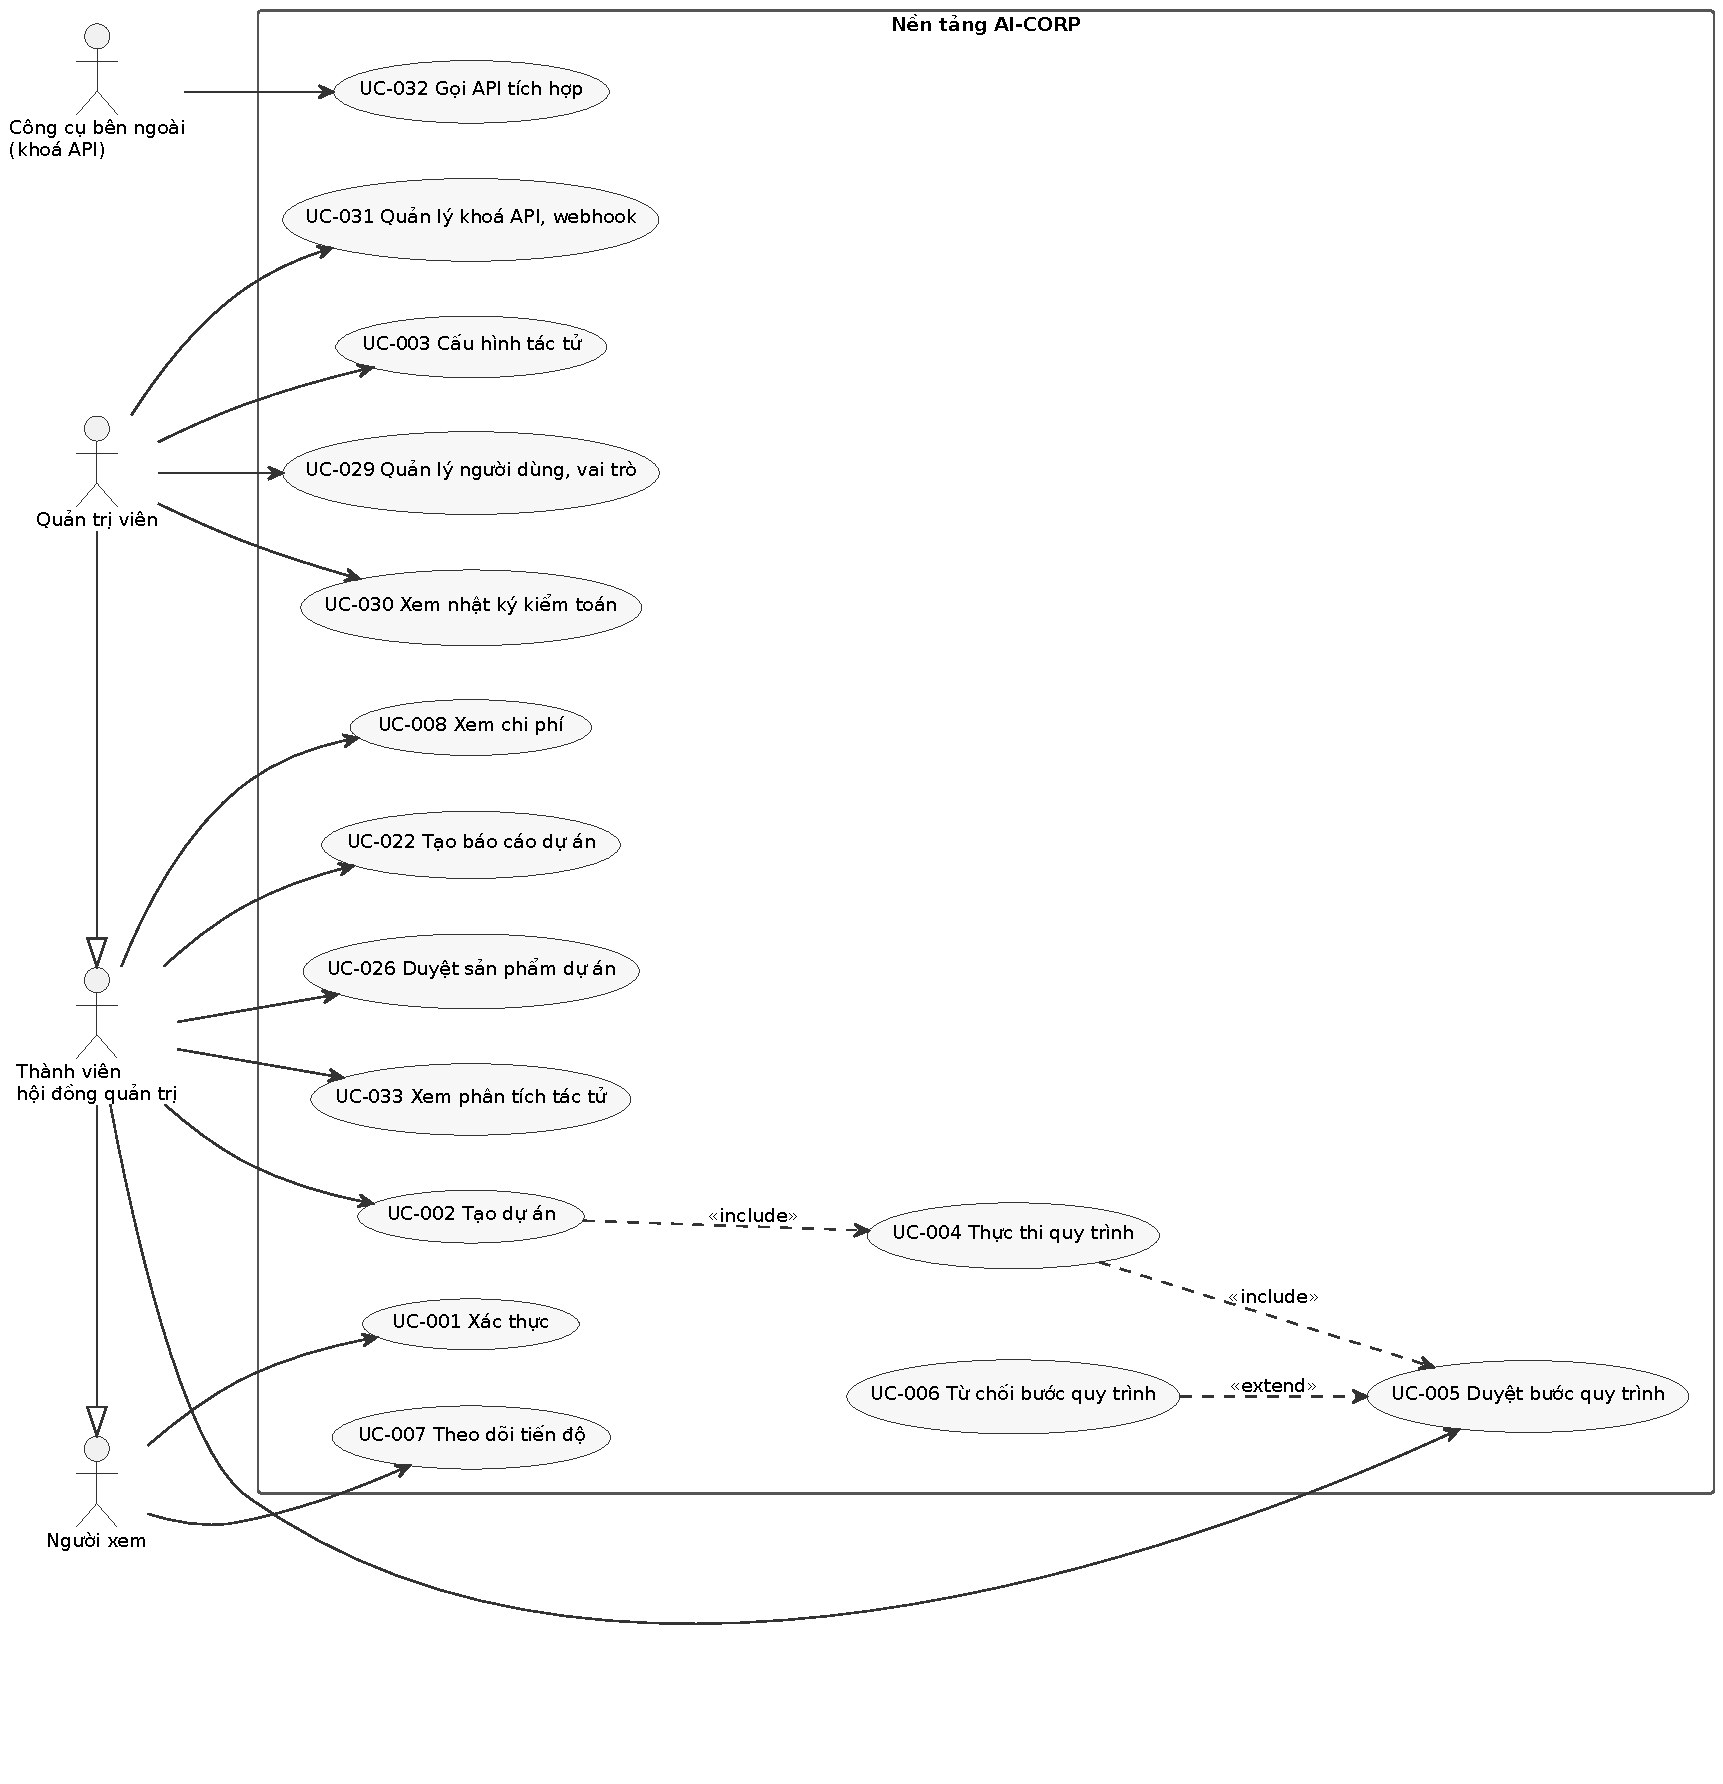
\includegraphics[width=0.92\textwidth]{sodo/use-case-con-nguoi.pdf}
\end{figure}

\begin{figure}{Sơ đồ use case phía tác tử và hệ thống}
\label{fig:uc-tac-tu}
\centering
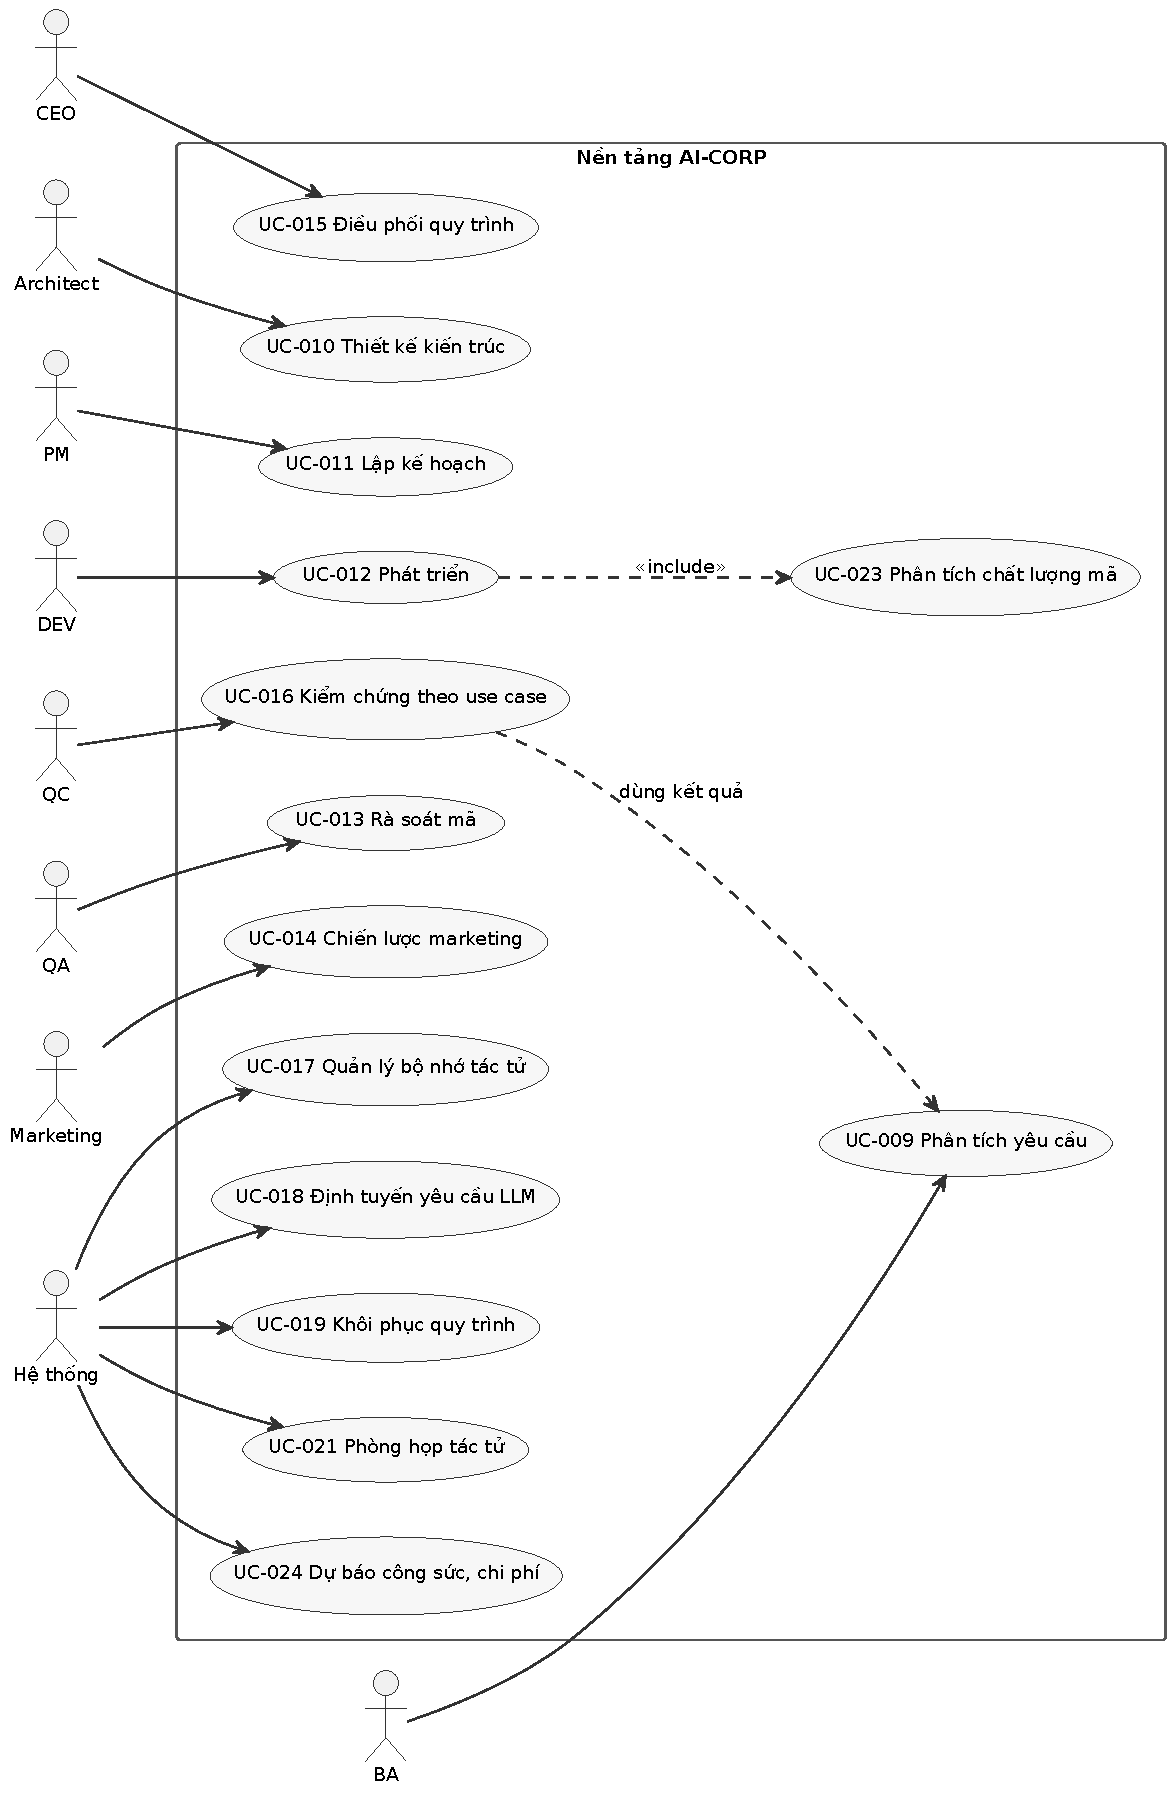
\includegraphics[width=0.68\textwidth]{sodo/use-case-tac-tu.pdf}
\end{figure}

Nhìn quan hệ giữa các use case sẽ thấy quy trình được dựng ra sao. UC-002 \textit{Tạo dự án} bao hàm UC-004 \textit{Thực thi quy trình}, vì tạo xong dự án thì quy trình chạy ngay. UC-004 bao hàm UC-005 \textit{Duyệt bước} khi quy trình có nút chờ con người, còn UC-006 \textit{Từ chối} mở rộng UC-005. UC-012 \textit{Phát triển} bao hàm UC-023 \textit{Phân tích chất lượng mã}, nơi hệ thống dự đoán phán quyết của QA và cho DEV sửa một vòng. UC-016 của QC lấy đầu ra của UC-009, tức các use case do BA viết, làm đầu vào.

\section{Đặc tả một số use case tiêu biểu}

Dưới đây là đặc tả của bốn use case đụng tới nhiều thành phần nhất. Các use case còn lại được viết theo cùng khuôn trong tài liệu yêu cầu.

\begin{table}{Đặc tả use case UC-002 Tạo dự án}
\label{tab:uc002}
\small
\begin{tabularx}{\textwidth}{|P{2.8cm}|L|}
\hline
\textbf{Tác nhân} & Thành viên hội đồng quản trị \\ \hline
\textbf{Tiền điều kiện} & Đã đăng nhập, có quyền \code{project:create} \\ \hline
\textbf{Luồng chính} &
(1) Người dùng chọn mẫu quy trình và điền tham số, ví dụ số use case tối thiểu, có bật bước phê duyệt hay không.
(2) Hệ thống kiểm tra mẫu và tham số trước khi tạo bất cứ thứ gì.
(3) Thực thể \code{Project} được tạo qua phương thức nhà máy \code{Project.create}, nơi các bất biến được áp: tên không rỗng, ngân sách dương.
(4) Dự án được lưu, sự kiện \code{ProjectCreatedEvent} được phát.
(5) Bộ máy quy trình tạo một lượt chạy gắn với phiên bản bất biến \code{mẫu@phiên_bản+băm} của định nghĩa quy trình.
(6) Hệ thống lưu một bản dự báo thời gian và chi phí lúc quy trình bắt đầu. \\ \hline
\textbf{Luồng thay thế} & Mẫu không tồn tại: trả 404. Tham số sai kiểu: trả 400 và chưa tạo dự án. Người xem gọi chức năng: trả 403 và ghi mục \code{access.denied} vào nhật ký kiểm toán. \\ \hline
\textbf{Hậu điều kiện} & Dự án ở trạng thái \code{active}, có một lượt chạy quy trình. Nhật ký kiểm toán có \code{project.create} và \code{workflow.started} \\ \hline
\end{tabularx}
\end{table}

\begin{table}{Đặc tả use case UC-004 Thực thi quy trình}
\label{tab:uc004}
\small
\begin{tabularx}{\textwidth}{|P{2.8cm}|L|}
\hline
\textbf{Tác nhân} & Hệ thống (bộ máy quy trình) và các tác tử \\ \hline
\textbf{Tiền điều kiện} & Dự án đang \code{active}, lượt chạy có định nghĩa quy trình hợp lệ \\ \hline
\textbf{Luồng chính} &
(1) Bộ máy kiểm tra ngân sách còn hay hết.
(2) Bộ máy lấy nút hiện tại và chọn chiến lược thực thi theo loại nút: \code{agent_task}, \code{sub_workflow}, \code{quality_gate}, \code{condition}, \code{parallel} hoặc \code{human_approval}.
(3) Chiến lược thực thi nút. Với nút tác tử, tác tử tương ứng chạy chu trình suy nghĩ và hành động.
(4) Bộ máy ghi một \code{WorkflowStep} kèm thời lượng, gộp kết quả vào ngữ cảnh lượt chạy và chụp ảnh trạng thái.
(5) Bộ máy chọn cạnh kế tiếp rồi lặp lại từ bước 1 cho tới khi gặp nút kết thúc. \\ \hline
\textbf{Luồng thay thế} & Nút lỗi được thử lại tối đa ba lần với thời gian chờ tăng theo hàm mũ. Vẫn lỗi thì đi theo cạnh \code{onFail}, nếu không có cạnh này thì lượt chạy chuyển \code{failed} và phát \code{workflow.failed}. Gặp nút phê duyệt: lượt chạy chuyển \code{paused}. Hết ngân sách: lượt chạy bị tạm dừng trước khi nút kế tiếp bắt đầu. \\ \hline
\textbf{Hậu điều kiện} & Lượt chạy ở \code{completed}, \code{paused}, \code{failed} hoặc \code{cancelled}. Mọi bước đã chạy đều có bản ghi và ảnh chụp \\ \hline
\end{tabularx}
\end{table}

\begin{table}{Đặc tả use case UC-005 Duyệt bước quy trình}
\label{tab:uc005}
\small
\begin{tabularx}{\textwidth}{|P{2.8cm}|L|}
\hline
\textbf{Tác nhân} & Thành viên hội đồng quản trị được giao phê duyệt \\ \hline
\textbf{Tiền điều kiện} & Lượt chạy đang dừng ở nút \code{human_approval} và có bản ghi \code{Approval} ở trạng thái \code{pending} \\ \hline
\textbf{Luồng chính} &
(1) Người dùng nhận thông báo, mở hộp thoại phê duyệt có tóm tắt sản phẩm.
(2) Người dùng bấm \textit{Approve}, giao diện gọi \code{POST /api/approvals/:id/approve}.
(3) Hệ thống kiểm tra quyền và kiểm tra người gọi đúng là người được giao.
(4) Hệ thống cập nhật phê duyệt với điều kiện trạng thái còn \code{pending}.
(5) Quyết định được ghi vào biến của lượt chạy và lượt chạy tiếp tục. \\ \hline
\textbf{Luồng thay thế} & Phê duyệt đã được trả lời trước đó: trả 409. Người không được giao hoặc người xem: trả 403, ghi \code{access.denied}. Từ chối (UC-006): bắt buộc nhập lý do, lý do được chuyển cho các tác tử chạy sau. \\ \hline
\textbf{Hậu điều kiện} & Phê duyệt có trạng thái cuối, nhật ký kiểm toán có \code{approval.approve} hoặc \code{approval.reject} \\ \hline
\end{tabularx}
\end{table}

\begin{table}{Đặc tả use case UC-016 Kiểm chứng hiện thực theo use case}
\label{tab:uc016}
\small
\begin{tabularx}{\textwidth}{|P{2.8cm}|L|}
\hline
\textbf{Tác nhân} & Tác tử QC \\ \hline
\textbf{Tiền điều kiện} & BA đã viết use case, DEV đã ghi mã vào kho tệp của dự án \\ \hline
\textbf{Luồng chính} &
(1) QC đọc use case của BA và mã của DEV.
(2) QC viết một tệp kiểm thử Jest cho mỗi use case, đặt tên \code{tests/UC-xxx.spec.ts}.
(3) Hệ thống chạy kiểm thử trong sandbox Docker, hoặc trong một bản sao tạm khi được phép chạy cục bộ.
(4) QC lập ma trận truy vết từ use case sang lớp, tệp hiện thực, tệp kiểm thử và kết quả.
(5) Độ bao phủ use case được ghi vào siêu dữ liệu OOAD của dự án. \\ \hline
\textbf{Hậu điều kiện} & Độ bao phủ chỉ tính kiểm thử đã chạy và đạt. Kiểm thử mới viết mà chưa chạy qua thì không tính. Use case chưa có kiểm thử được liệt kê là còn thiếu. \\ \hline
\end{tabularx}
\end{table}

Ở UC-005, bước (4) nhìn thì hiển nhiên nhưng lại là chỗ dễ sai nhất. Nếu hệ thống đọc trạng thái, thấy \code{pending}, rồi mới ghi, thì hai yêu cầu đến gần như cùng lúc sẽ cùng thấy \code{pending} và cùng ghi thành công. Lỗi này đã xảy ra thật, và chương~\ref{chap:kiem-thu} kể lại nó được sửa thế nào.

\section{Mô hình miền}

Mô hình miền của nền tảng xoay quanh ba aggregate chính, thể hiện ở Hình~\ref{fig:mo-hinh-mien}:

\begin{itemize}
\item \textbf{Project} là gốc aggregate, chứa các \code{Milestone} và \code{Task}. Ngân sách và chi phí đã tiêu được biểu diễn bằng value object \code{Money}. Trạng thái \code{ProjectStatus} cũng là một value object có quy tắc chuyển trạng thái riêng.
\item \textbf{Agent} có vai trò \code{AgentRole}, cấu hình mô hình LLM, bộ nhớ \code{AgentMemory} và máy trạng thái vòng đời.
\item \textbf{WorkflowRun} tham chiếu tới một phiên bản bất biến của định nghĩa quy trình, chứa các \code{WorkflowStep} và ảnh chụp \code{WorkflowSnapshot}, có thể có lượt chạy cha (khi là quy trình con) và các \code{Approval}.
\end{itemize}

Xung quanh còn có các khái niệm phụ trợ. Có \code{User} và \code{Role}, có \code{AuditLog} chỉ cho ghi thêm chứ không cho sửa. Có \code{ApiKey}, \code{Webhook} và \code{WebhookDelivery}, có \code{ApiUsageLog} lưu chi phí từng lời gọi LLM, rồi \code{QualityGateLog} và \code{ProjectEstimate}. Cuối cùng là aggregate \code{LlmProviderConfig} quản lý danh sách \code{LlmModel} của nó.

\begin{figure}{Mô hình miền rút gọn của nền tảng}
\label{fig:mo-hinh-mien}
\centering
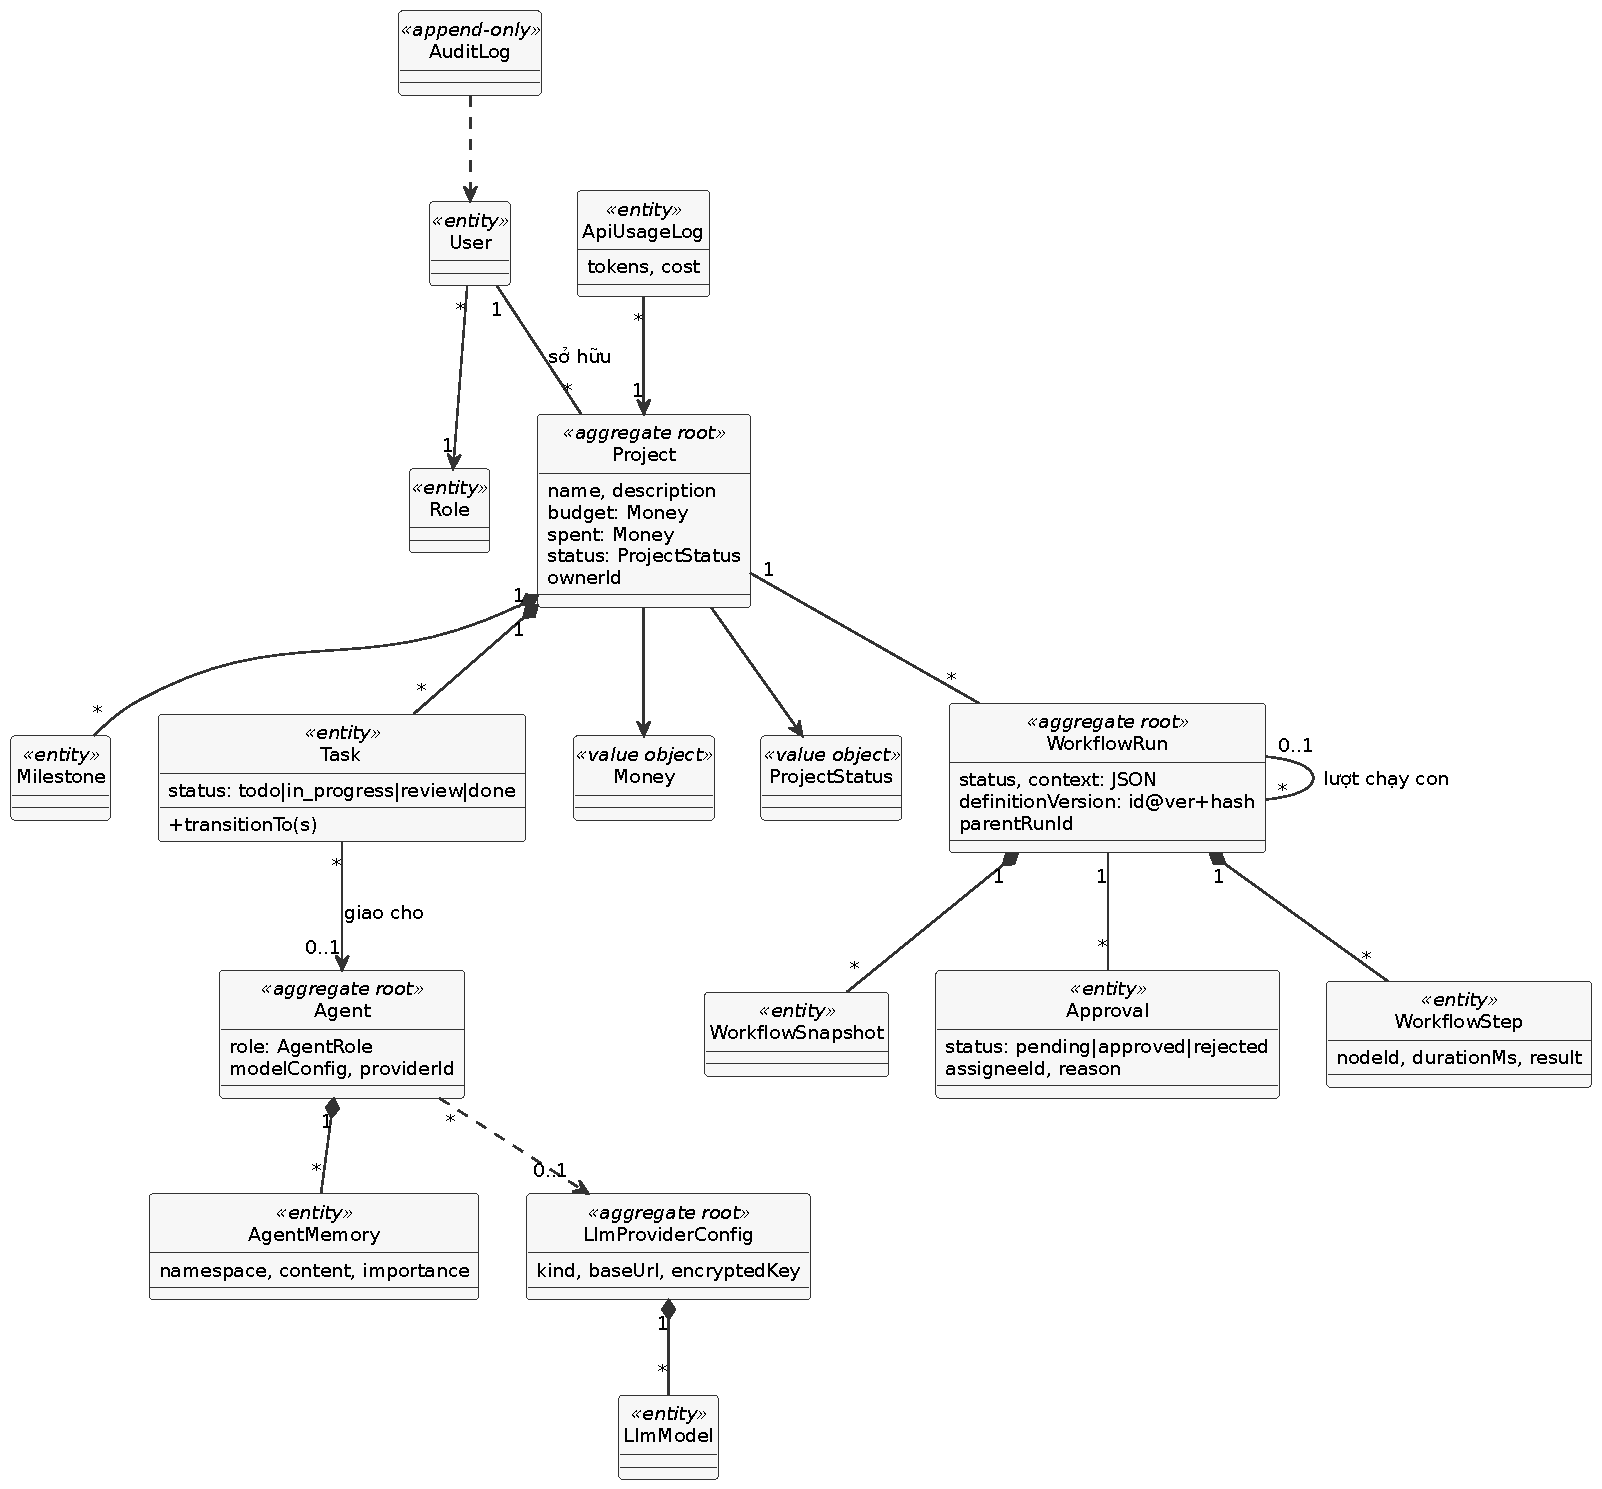
\includegraphics[width=\textwidth]{sodo/mo-hinh-mien.pdf}
\end{figure}

\chapter{Thiết kế hệ thống}
\label{chap:thiet-ke}

Chương này đi từ cái chung tới cái riêng. Đầu tiên là kiến trúc và các mẫu thiết kế, sau đó tới tác tử, bộ máy quy trình, dữ liệu, cách áp OOAD vào dự án sinh ra, bảo mật, phân tích và dự báo, cuối cùng là triển khai. Đủ 39 sơ đồ UML gốc được liệt kê ở Phụ lục~\ref{app:uml}. Các hình trong chương này được vẽ lại gọn hơn cho vừa khổ giấy.

\section{Kiến trúc tổng thể}

\subsection{Kiểu kiến trúc}

Nền tảng gồm một máy chủ API viết bằng NestJS và TypeScript, cùng một ứng dụng web một trang viết bằng React. Bên trong API, mã nguồn chia thành bốn tầng theo kiến trúc phân lớp kết hợp thiết kế hướng miền~\cite{evans2003,martin2017}. Bảng~\ref{tab:tang} cho biết mỗi tầng chứa gì và được phép dựa vào tầng nào.

\begin{table}{Bốn tầng của API và quy tắc phụ thuộc}
\label{tab:tang}
\small
\begin{tabularx}{\textwidth}{|P{2.6cm}|L|P{3.2cm}|}
\hline
\textbf{Tầng} & \textbf{Nội dung} & \textbf{Được phụ thuộc vào} \\ \hline
Trình bày & Controller REST, cổng WebSocket (Socket.IO), DTO, guard & Ứng dụng \\ \hline
Ứng dụng & Dịch vụ ứng dụng (mỗi use case một phương thức), chiến lược tác tử, bộ máy quy trình, bộ xử lý sự kiện & Miền \\ \hline
Miền (\code{src/domain}) & Thực thể, value object, aggregate, sự kiện miền, máy trạng thái, giao diện Repository, các cổng, chính sách thuần không có I/O & Không phụ thuộc tầng nào \\ \hline
Hạ tầng & Repository Prisma, nhà cung cấp LLM, sandbox Docker, kho tệp dự án, bộ phân tích mã TypeScript, xuất PDF & Miền (hiện thực các cổng) \\ \hline
\end{tabularx}
\end{table}

Tầng miền có 106 tệp và không nhập NestJS, Prisma hay thư viện I/O nào. Vì thế các quy tắc nghiệp vụ như chuyển trạng thái công việc, cộng trừ tiền, phát hiện bất thường, hồi quy dự báo hay chấm điểm chất lượng mã đều kiểm thử được như hàm thuần, không phải dựng framework hay cơ sở dữ liệu. Ngưỡng độ bao phủ cao nhất cũng đặt ở tầng này. Trên Hình~\ref{fig:kien-truc}, mọi mũi tên phụ thuộc đều chỉ vào tầng miền, còn tầng hạ tầng hiện thực các giao diện do tầng miền khai báo.

\begin{figure}{Kiến trúc phân lớp của API}
\label{fig:kien-truc}
\centering
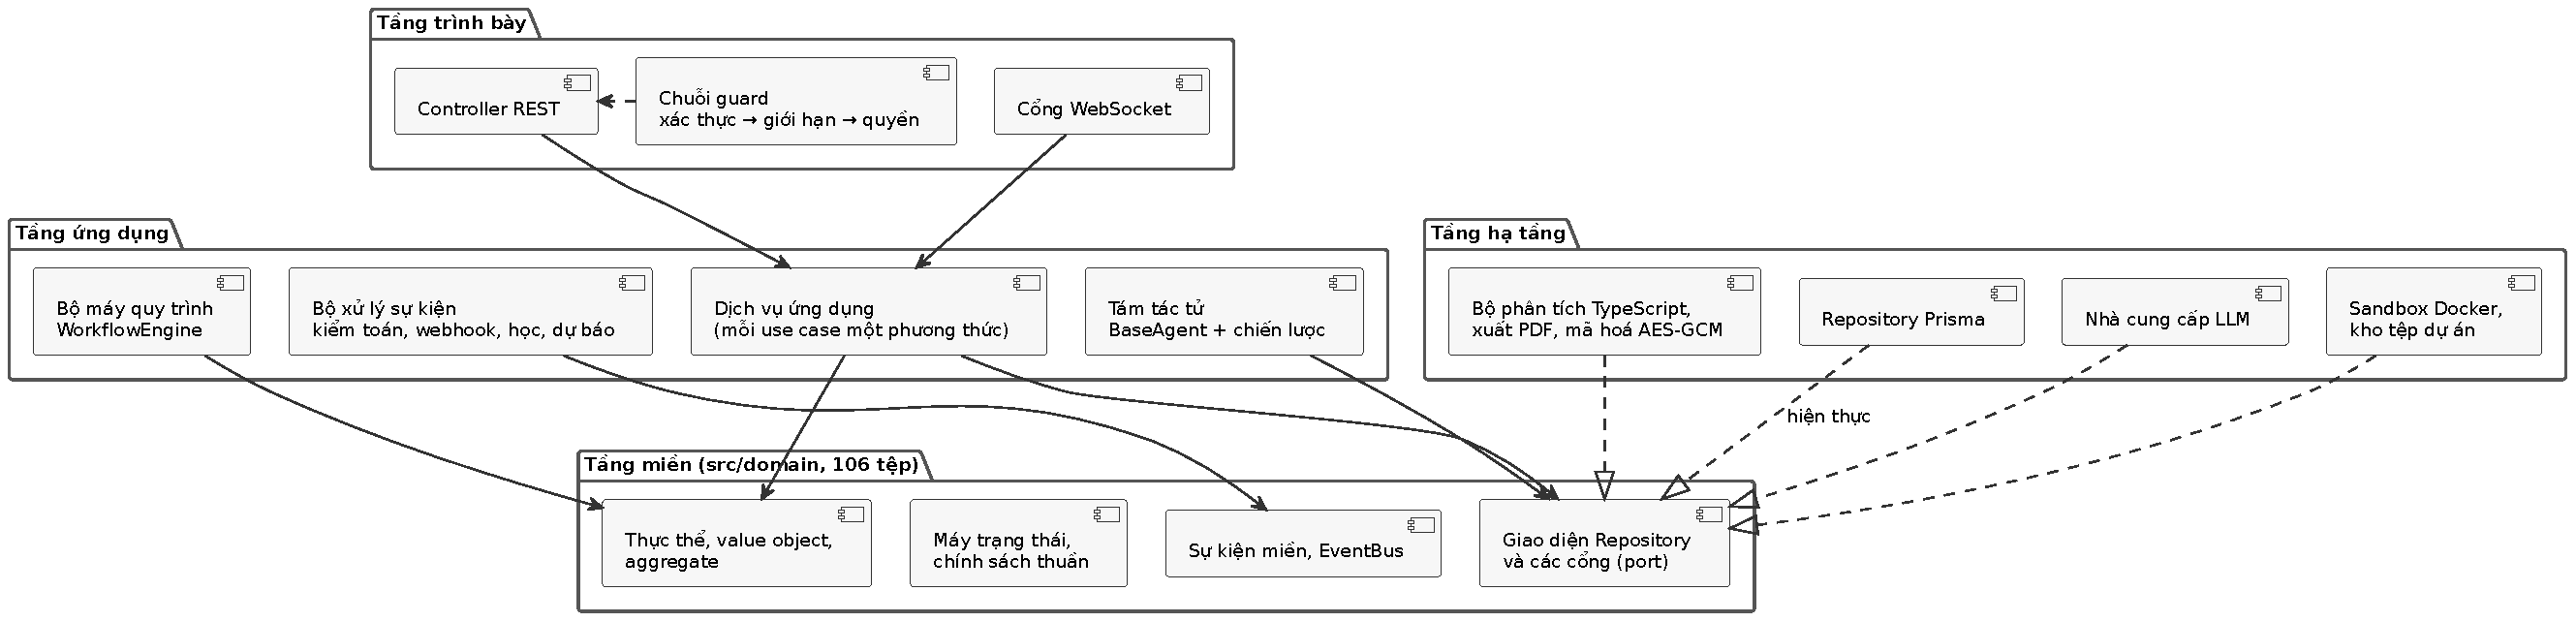
\includegraphics[width=\textwidth]{sodo/kien-truc-phan-lop.pdf}
\end{figure}

\subsection{Các quyết định kiến trúc chính}

Mỗi quyết định kiến trúc được ghi thành một bản ghi quyết định kiến trúc (ADR) trong \code{docs/design/architecture.md}. Sáu quyết định có tác động lớn nhất như sau:

\begin{enumerate}
\item \textbf{Chọn NestJS cho API.} NestJS có sẵn cơ chế tiêm phụ thuộc và hệ thống mô-đun, tức là làm sẵn nguyên lý DIP. Nó còn cho đăng ký nhiều hiện thực dưới cùng một token, và nền tảng tận dụng điều này cho danh sách tác tử và danh sách chiến lược nút.
\item \textbf{Chọn PostgreSQL} cho cả dữ liệu quan hệ lẫn dữ liệu JSON như ngữ cảnh lượt chạy hay siêu dữ liệu OOAD, với Prisma làm lớp ánh xạ nằm sau các Repository.
\item \textbf{Chọn BullMQ trên Redis} làm hàng đợi cho các nút quy trình. Thiếu Redis thì bộ máy chạy nút trực tiếp. Điểm kiểm tra tình trạng khi đó báo \textit{degraded} nhưng hệ thống vẫn chạy.
\item \textbf{Mọi truy cập dữ liệu từ tầng ứng dụng đi qua Repository}, nên dịch vụ ứng dụng kiểm thử được bằng Repository lưu trong bộ nhớ.
\item \textbf{Chuyên môn hoá tác tử bằng Strategy} thay cho cây kế thừa sâu (mục~\ref{sec:tk-tac-tu}).
\item \textbf{Các mô-đun nói chuyện với nhau qua sự kiện miền.} Kiểm toán, webhook, cơ chế học, dự báo và giám sát bất thường đều chỉ nghe sự kiện, không gọi thẳng vào nhau.
\end{enumerate}

\section{Mẫu thiết kế}
\label{sec:mau}

Bảng~\ref{tab:mau-1} và Bảng~\ref{tab:mau-2} ghép mỗi mẫu thiết kế với vấn đề nó giải quyết và lớp hiện thực nó. Lớp nào trong mã cũng có chú thích \code{@pattern}, nên người đọc có thể tìm trong kho mã để so từng dòng của bảng.

\begin{table}{Mẫu thiết kế trong nền tảng (phần 1: tác tử và quy trình)}
\label{tab:mau-1}
\footnotesize
\begin{tabularx}{\textwidth}{|L|P{2.7cm}|P{5.3cm}|}
\hline
\textbf{Vấn đề} & \textbf{Mẫu} & \textbf{Hiện thực} \\ \hline
Tám vai trò có chung chu trình nhận việc, suy nghĩ, hành động, hoàn tất & Template Method & \code{BaseAgent.execute()} \\ \hline
Mỗi vai trò suy nghĩ và hành động khác nhau, cần thay được độc lập & Strategy & \code{IThinkingStrategy}, \code{IActionStrategy}, 16 lớp chiến lược \\ \hline
Thêm vai trò mà không sửa bộ điều phối & Registry + DIP & \code{AgentOrchestrator} nhận danh sách \code{IAgent} qua token \code{AGENTS}; mỗi vai trò một \code{RoleProfile} \\ \hline
Tác tử, công việc, dự án, phê duyệt chỉ được chuyển trạng thái hợp lệ & State & \code{AgentStateMachine}, \code{Task.transitionTo}, value object \code{ProjectStatus} \\ \hline
Nhiều bên cần biết khi tác tử đổi trạng thái hoặc xong việc & Observer & \code{AgentEventEmitter}, \code{IAgentObserver}; \code{EventBus} và các handler \\ \hline
Mỗi loại nút chạy khác nhau, thêm loại nút không sửa bộ máy & Strategy tự đăng ký & \code{NodeExecutionStrategy}: tác tử, quy trình con, cổng chất lượng, điều kiện, song song, phê duyệt, cộng tác \\ \hline
Một nút là cả một quy trình & Composite & \code{SubWorkflowStrategy} chạy quy trình con thành lượt chạy con \\ \hline
Quay lại trạng thái trước của lượt chạy & Memento & \code{WorkflowRunMemento}, \code{WorkflowSnapshotCaretaker} \\ \hline
Định nghĩa quy trình không bị sửa khi đã có lượt chạy dùng nó & Sổ đăng ký bất biến & \code{WorkflowDefinitionRegistry} theo khoá \code{id@phiên_bản+băm} \\ \hline
Tác tử trao đổi thông điệp có kiểu khi cộng tác & Mediator & \code{AgentMessageBus}, \code{EventBus} \\ \hline
\end{tabularx}
\end{table}

\begin{table}{Mẫu thiết kế trong nền tảng (phần 2: LLM, bảo mật, báo cáo, chất lượng)}
\label{tab:mau-2}
\footnotesize
\begin{tabularx}{\textwidth}{|L|P{2.7cm}|P{5.3cm}|}
\hline
\textbf{Vấn đề} & \textbf{Mẫu} & \textbf{Hiện thực} \\ \hline
Ghi chi phí mọi lời gọi LLM mà không sửa nhà cung cấp & Decorator & \code{UsageTrackingLLMProvider} \\ \hline
Tác tử gọi LLM qua một cửa duy nhất & Facade & \code{AgentLLMService}, \code{OoadArtifactService}, \code{CodeQualityService} \\ \hline
Nhiều nhà cung cấp LLM sau một giao diện & Adapter + Factory Method & \code{ILLMProvider}, \code{LLMProviderFactory} \\ \hline
Quản trị viên thêm nhà cung cấp, mô hình lúc hệ thống đang chạy & Aggregate + Strategy + Registry & \code{LlmProviderConfig} chứa \code{LlmModel}; \code{ProviderStrategy} cho mỗi loại; \code{ProviderStrategyRegistry}, \code{ConfiguredProviderRegistry} \\ \hline
Mã hoá khoá API của nhà cung cấp mà tầng miền không phụ thuộc thư viện mật mã & Port/Adapter & \code{SecretCipher} (miền), \code{AesGcmSecretCipher} (hạ tầng) \\ \hline
Một phê duyệt chỉ được trả lời một lần dù có hai yêu cầu đồng thời & Cập nhật có điều kiện & \code{ApprovalService}: chỉ cập nhật khi trạng thái còn \code{pending} \\ \hline
Xác thực, giới hạn tần suất rồi mới kiểm tra quyền & Chain of Responsibility & \code{AuthenticationGuard}, \code{RateLimitGuard}, \code{PermissionGuard}; chuỗi rà soát QC rồi QA \\ \hline
Biến sự kiện miền thành mục kiểm toán hoặc payload webhook & Adapter & \code{AuditLogHandler}, \code{webhook-payloads} \\ \hline
Tách truy cập dữ liệu khỏi miền & Repository, Data Mapper & \code{I*Repository} ở miền, \code{Prisma*Repository} ở hạ tầng \\ \hline
Dựng báo cáo chi phí, hiệu năng theo từng bước & Builder & \code{CostReportBuilder}, \code{PerformanceReportBuilder} \\ \hline
Xuất JSON, CSV, PDF tuỳ định dạng & Strategy + Registry & \code{ProjectExportService} và ba exporter \\ \hline
Mỗi loại bất thường, mỗi tín hiệu chất lượng là một quy tắc & Strategy + Composite & \code{IAgentAnomalyRule}, \code{IQualitySignal}, \code{AgentAnomalyDetector} \\ \hline
Phân tích mã sinh ra mà miền không phụ thuộc trình biên dịch & Port/Adapter & \code{ICodeAnalyzer} (miền), \code{TypeScriptCodeAnalyzer} (hạ tầng) \\ \hline
Quy tắc chấm điểm chất lượng mã & Policy, Specification & \code{CodeQualityPolicy}, \code{LayerRules} \\ \hline
\end{tabularx}
\end{table}

\section{Thiết kế tác tử}
\label{sec:tk-tac-tu}

\subsection{Một khung chung, hai chiến lược riêng}

Mỗi tác tử là một đối tượng \code{BaseAgent} lắp từ ba phần (Hình~\ref{fig:lop-tac-tu}). Phần thứ nhất là \code{RoleProfile}, mô tả vai trò, các loại công việc vai trò làm được và lời nhắc hệ thống. Hai phần còn lại là một chiến lược tư duy và một chiến lược hành động. Phương thức \code{BaseAgent.execute()} giữ cố định khung thuật toán như sau:

\begin{enumerate}
\item Chuẩn hoá ngữ cảnh. Loại công việc được so với hồ sơ vai trò, nên chiến lược lúc nào cũng nhận đúng loại việc mà vai trò đó làm được.
\item Phát sự kiện \code{TaskAssignedEvent}.
\item Chuyển \code{IDLE} sang \code{THINKING} rồi gọi \code{thinkingStrategy.think(context)}. Ở bước này, chiến lược nạp bộ nhớ, nạp bài học liên quan và gọi LLM để lập kế hoạch.
\item Chuyển \code{THINKING} sang \code{ACTING} rồi gọi \code{actionStrategy.act(context, thought)}. Chiến lược sinh tài liệu hoặc mã, ghi vào kho tệp của dự án và chạy các công cụ cần thiết.
\item Chuyển sang \code{COMPLETED} rồi về \code{IDLE}, lưu ký ức và phát \code{AgentCompletedTaskEvent}.
\item Nếu có ngoại lệ, tác tử chuyển sang \code{ERROR}. Với lỗi tạm thời, tác tử được quay về \code{IDLE}.
\end{enumerate}

\begin{figure}{Sơ đồ lớp của tác tử: Template Method kết hợp hai Strategy}
\label{fig:lop-tac-tu}
\centering
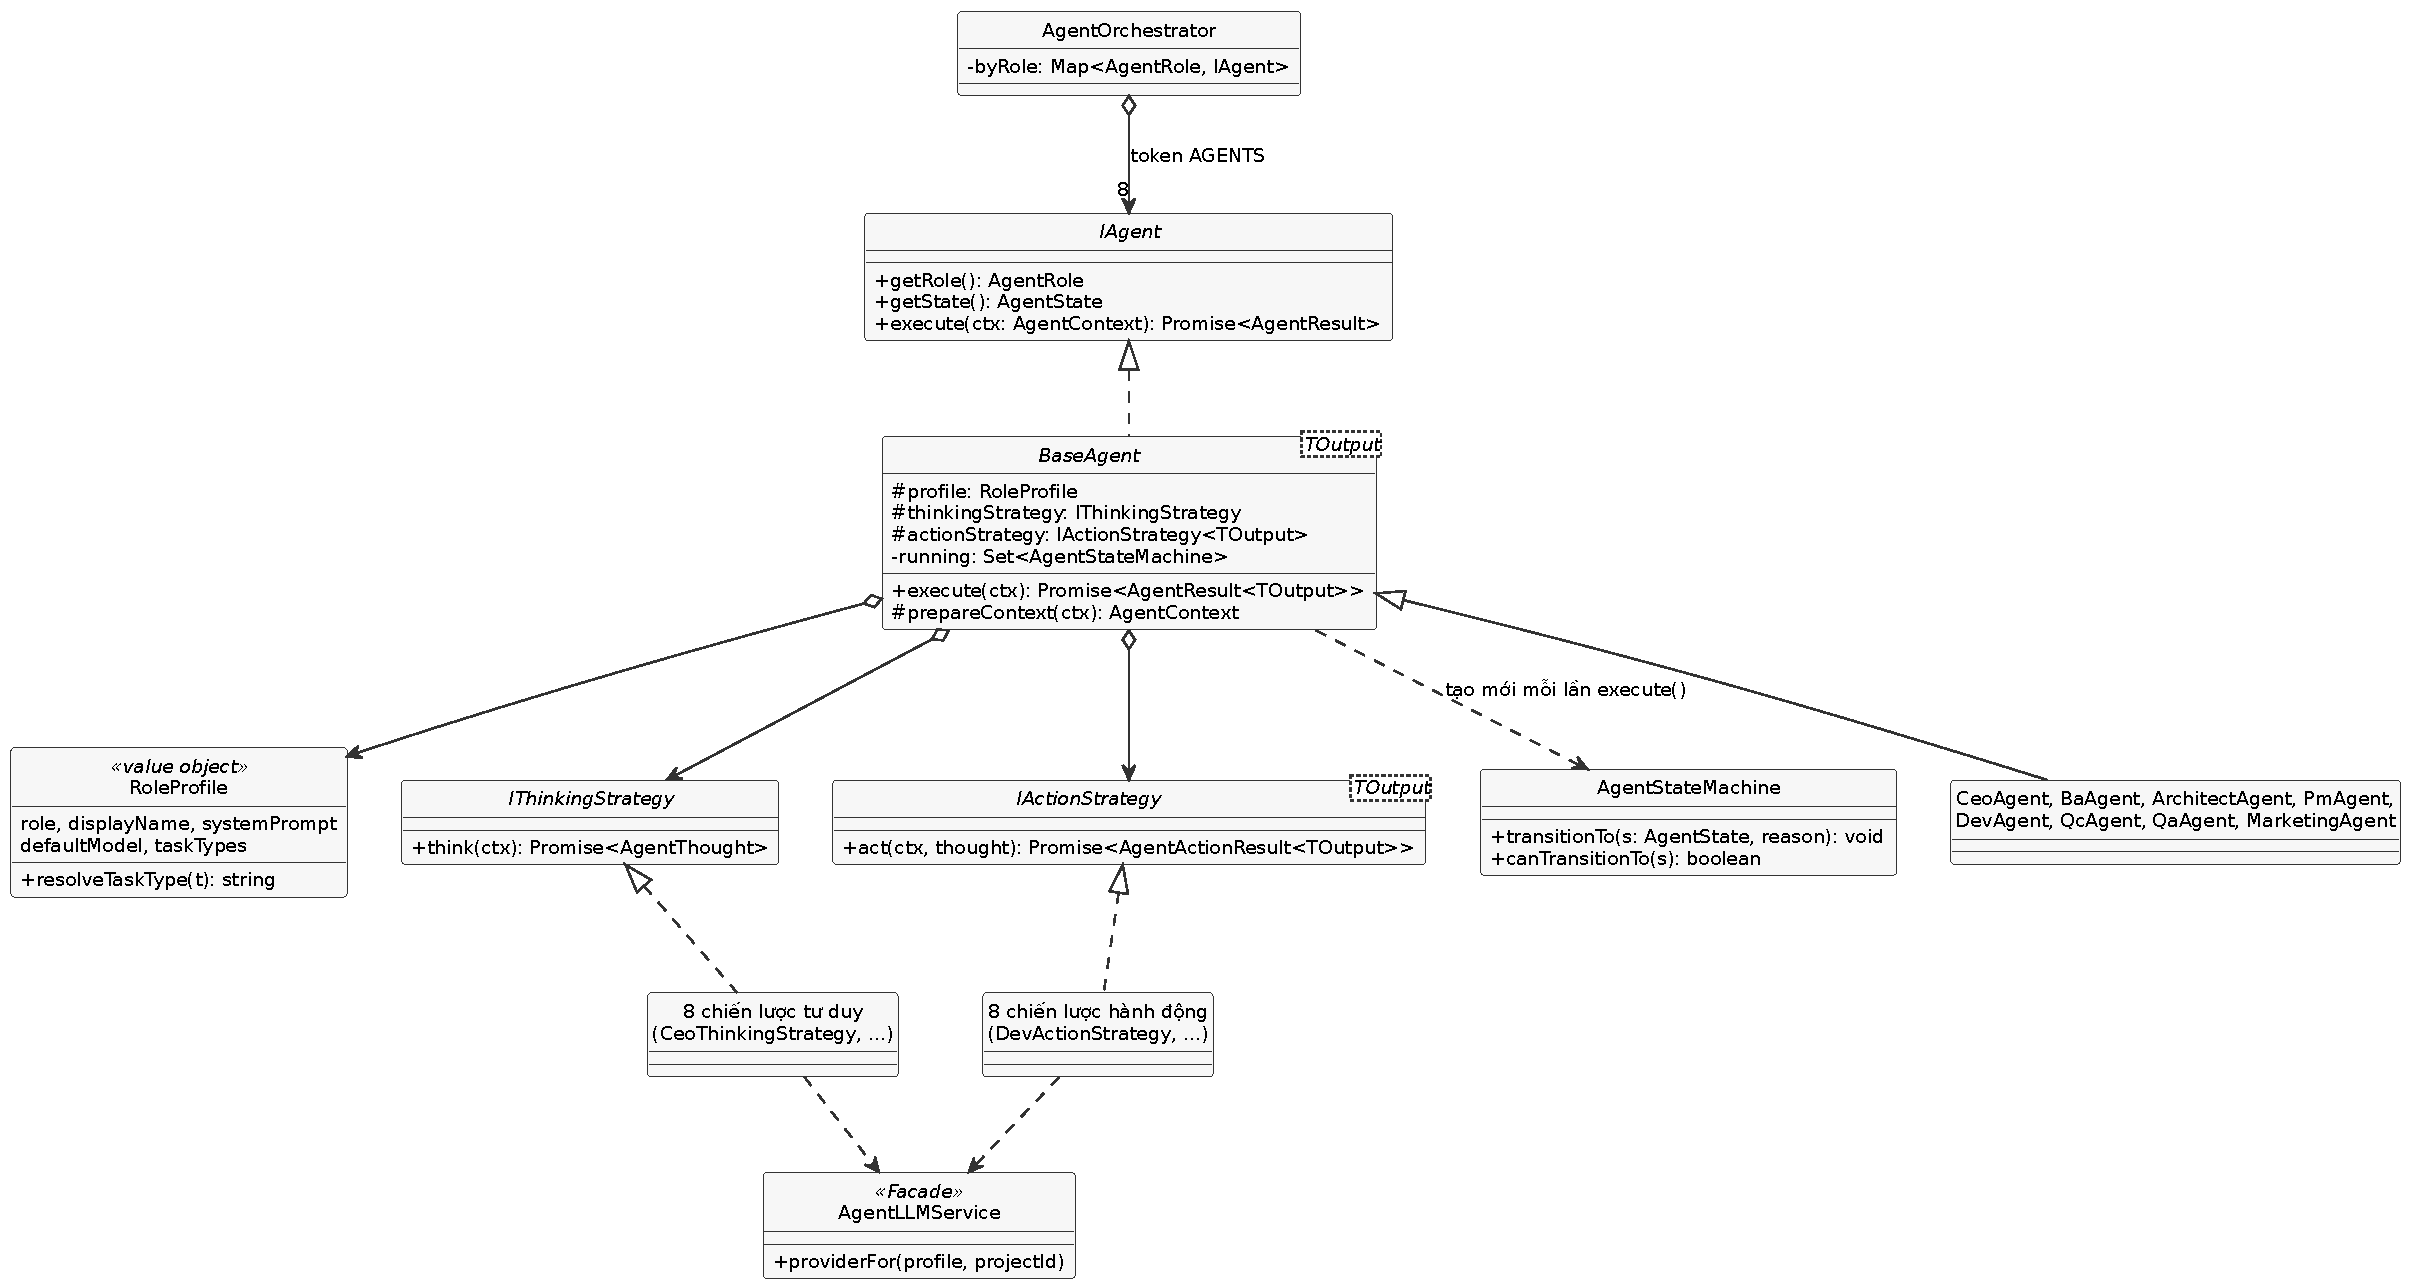
\includegraphics[width=\textwidth]{sodo/lop-tac-tu.pdf}
\end{figure}

Chia như vậy thì thoả ba nguyên lý SOLID. Tác tử chỉ lo vòng đời, chuyên môn để trong chiến lược, nên lớp nào cũng chỉ có một lý do để sửa (SRP). Muốn thêm vai trò thì thêm một hồ sơ và hai chiến lược, không phải đụng vào mã cũ (OCP). Mọi tác tử đều thay thế được cho nhau qua giao diện \code{IAgent}, nên bộ điều phối không cần biết mình đang gọi CEO hay QC (LSP).

\subsection{Máy trạng thái gắn với từng lần thực thi}

Thiết kế ban đầu cho mỗi vai trò giữ đúng một máy trạng thái. Lúc kiểm thử, cách này gây ra hai chuyện. Một là khi hai công việc cùng vai trò chạy song song, chúng ghi đè trạng thái của nhau và sinh lỗi ``Invalid state transition: IDLE → ERROR''. Hai là sau một lỗi không phục hồi được, vai trò đó kẹt luôn ở \code{ERROR} và từ chối mọi việc giao sau đó.

Sau khi sửa, mỗi lần gọi \code{execute()} có một máy trạng thái riêng. Tác tử giữ tập các máy trạng thái đang chạy và báo ra trạng thái của lần thực thi gần nhất (Hình~\ref{fig:sm-tac-tu}). Bài học ở đây về mẫu State là máy trạng thái phải gắn với thứ thật sự có vòng đời, ở đây là một lần thực thi, chứ không gắn vào một đối tượng sống lâu như chính tác tử.

\begin{figure}{Máy trạng thái của một lần thực thi tác tử}
\label{fig:sm-tac-tu}
\centering
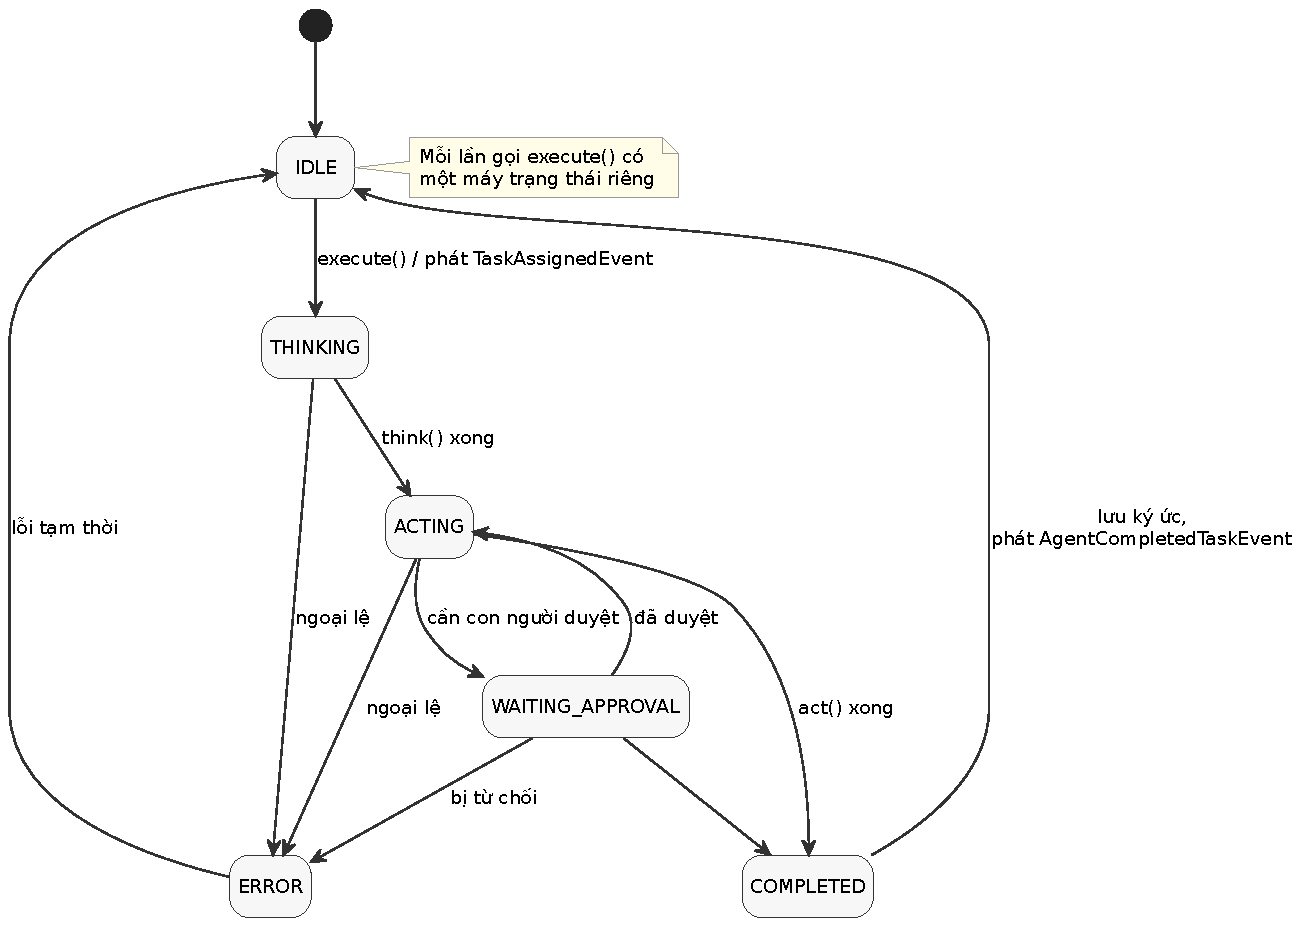
\includegraphics[width=0.78\textwidth]{sodo/may-trang-thai-tac-tu.pdf}
\end{figure}

\subsection{Gọi LLM và ghi chi phí}
\label{subsec:llm}

Chiến lược không gọi thẳng nhà cung cấp LLM mà đi qua \code{AgentLLMService}, một Facade. Lớp này tra cấu hình mô hình của vai trò, lấy nhà cung cấp từ \code{LLMProviderFactory}, rồi bọc nhà cung cấp trong \code{UsageTrackingLLMProvider} theo mẫu Decorator. Decorator chuyển nguyên lời gọi xuống lớp bên trong. Có kết quả rồi, nó ghi số token và chi phí vào \code{ApiUsageLog}, cộng vào chi phí dự án và phát \code{BudgetExceededEvent} đúng một lần khi vượt ngân sách. Nhờ thế chi phí của cả tám vai trò đều được ghi đủ, và không chiến lược nào phải tự tính tiền.

Nhà cung cấp và mô hình LLM được quản lý ngay trong ứng dụng, bên cạnh cách cấu hình bằng biến môi trường (Hình~\ref{fig:lop-llm}). \code{LlmProviderConfig} là gốc aggregate. Nó quản lý danh sách \code{LlmModel}, tự kiểm tra các bất biến (tên dài từ 1 đến 60 ký tự, URL http hoặc https hợp lệ, loại nhà cung cấp đã được hỗ trợ, không trùng mô hình) và chỉ lưu khoá API ở dạng đã mã hoá. Việc mã hoá đi qua cổng \code{SecretCipher} của tầng miền, còn tầng hạ tầng hiện thực cổng này bằng AES-256-GCM với khoá \code{LLM_SECRET_KEY}. API chỉ trả về bốn ký tự cuối của khoá. Mỗi loại nhà cung cấp, hiện là tương thích OpenAI và Anthropic, là một \code{ProviderStrategy} biết tạo client, kiểm tra kết nối và lấy danh sách mô hình. Muốn hỗ trợ thêm loại mới thì chỉ việc thêm một chiến lược vào sổ đăng ký.

Cấu hình mô hình của mỗi vai trò có thêm trường \code{providerId}. \code{LLMProviderFactory} hỏi \code{ConfiguredProviderRegistry} để lấy client đã cấu hình (có bộ đệm), hoặc dùng cổng mặc định khi vai trò chưa chọn nhà cung cấp. Lần khởi động đầu tiên, nếu bảng nhà cung cấp còn trống, hệ thống lấy cổng LLM khai báo trong biến môi trường làm nhà cung cấp đầu tiên, để bản cài đặt cũ khỏi phải cấu hình lại. Khi thêm tính năng này, tác tử, chiến lược và decorator ghi chi phí không phải sửa dòng nào, vì chúng chỉ biết tới giao diện \code{ILLMProvider}.

\begin{figure}{Sơ đồ lớp của phần quản lý nhà cung cấp LLM}
\label{fig:lop-llm}
\centering
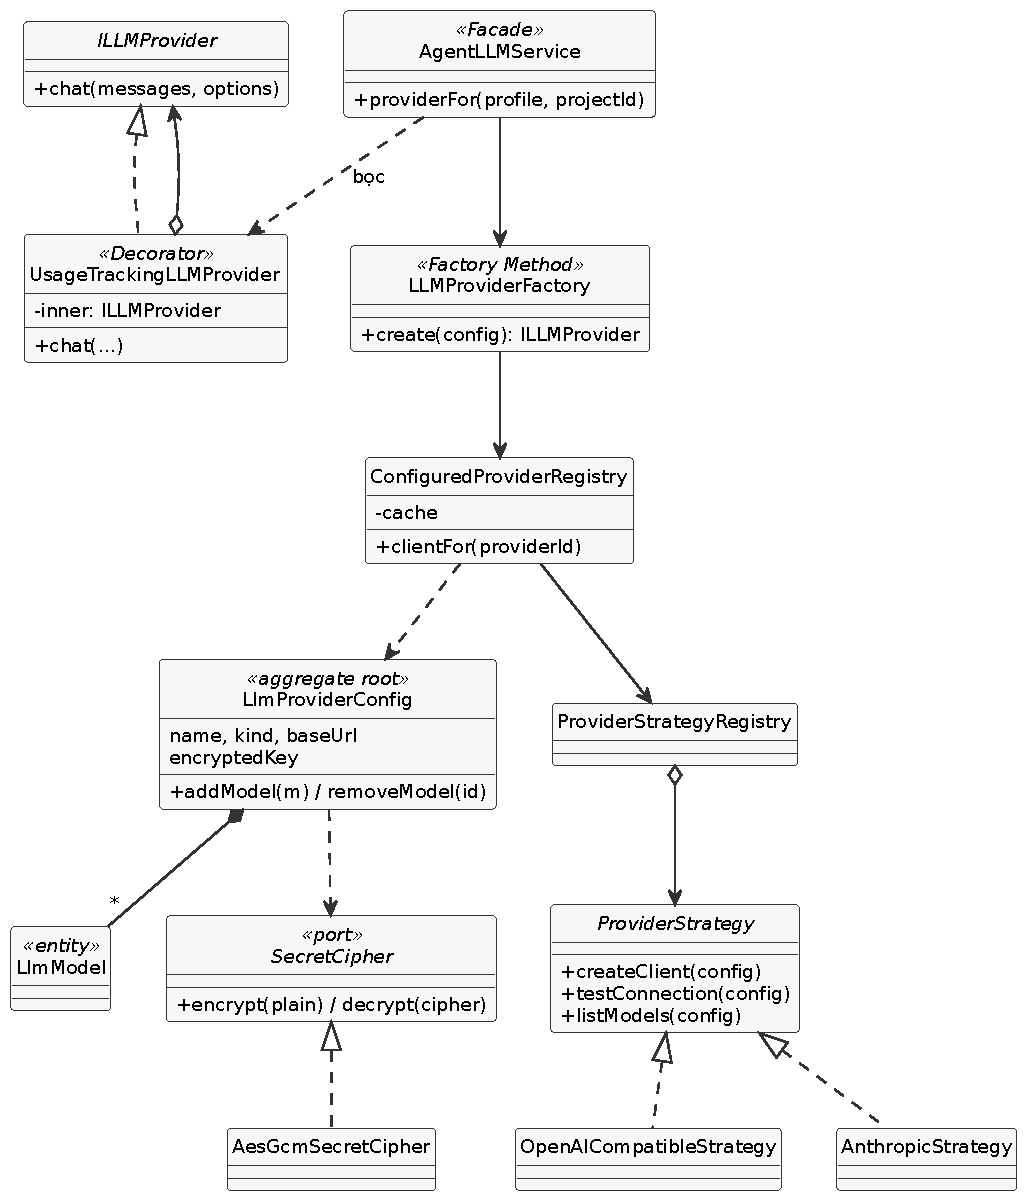
\includegraphics[width=0.72\textwidth]{sodo/lop-nha-cung-cap-llm.pdf}
\end{figure}

\subsection{Học từ kết quả}
\label{subsec:hoc}

Cơ chế học gồm ba phần (Hình~\ref{fig:tuan-tu-hoc}):

\begin{enumerate}
\item \code{OutcomeSignalPolicy} là một chính sách thuần, quyết định tín hiệu nào dùng để chấm lần thực thi nào. Kết quả cổng OOAD dùng để chấm BA và Architect. Kết quả của QC (số kiểm thử đạt, use case còn thiếu) dùng để chấm DEV. Phán quyết của QA chấm cả DEV và QC.
\item \code{LearningService} lưu từng kết quả vào bộ nhớ của vai trò. Cứ đủ N kết quả (mặc định là 3), dịch vụ gọi LLM để tóm các kết quả gần đây lại thành một ký ức loại \code{lessons_learned}. Lời gọi này cũng bị tính tiền như mọi lời gọi khác.
\item Khi dựng lời nhắc, chiến lược tư duy nạp các bài học này trước tiên.
\end{enumerate}

\begin{figure}{Tuần tự của chu trình học từ kết quả}
\label{fig:tuan-tu-hoc}
\centering
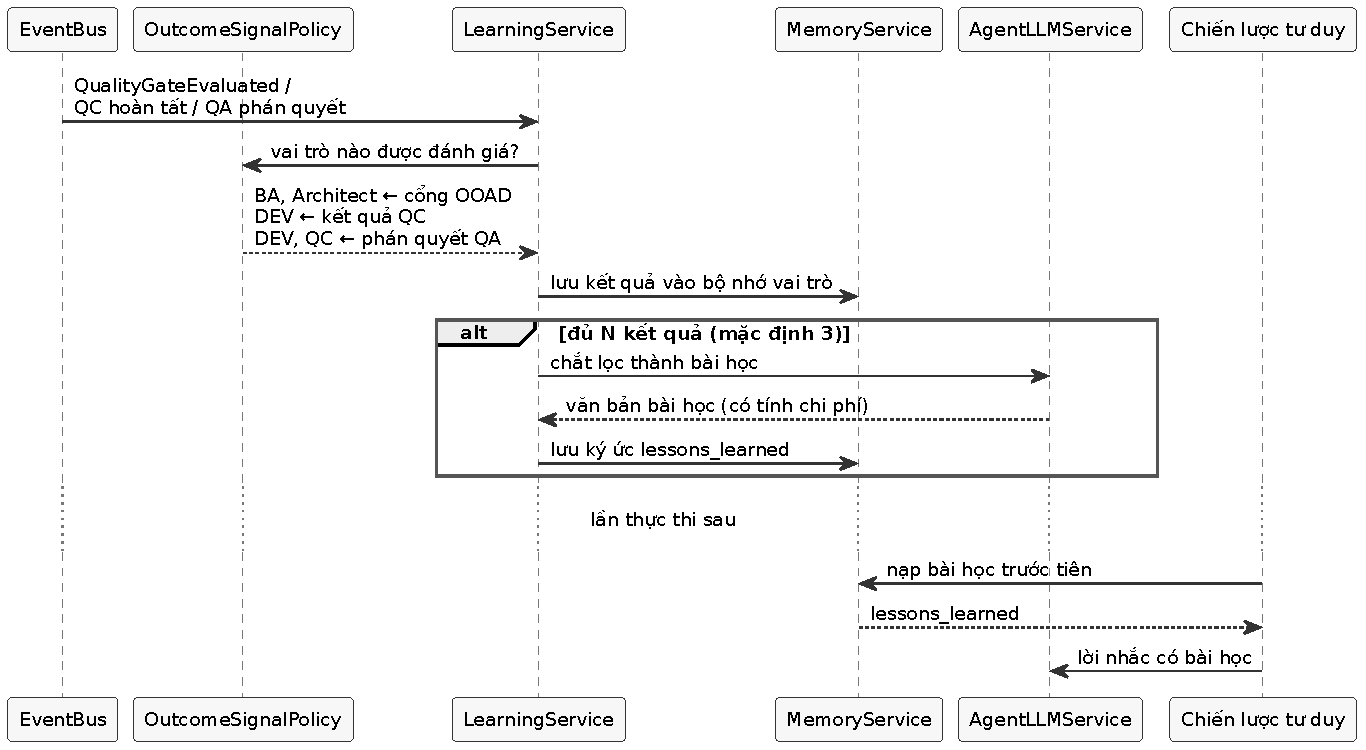
\includegraphics[width=0.85\textwidth]{sodo/tuan-tu-hoc.pdf}
\end{figure}

Thiết kế này giống Reflexion~\cite{shinn2023} ở chỗ phản hồi được viết bằng lời. Chỗ khác là tín hiệu chấm điểm đến từ một nguồn khách quan bên ngoài tác tử, còn ở Reflexion tác tử tự chấm chính mình.

\subsection{Cộng tác giữa các tác tử}

Có ba kiểu cộng tác. Mỗi kiểu là chiến lược của một nút quy trình và được đăng ký trong \code{CollaborationRegistry}:

\begin{itemize}
\item \textbf{Lập trình cặp} (\code{pair_develop}). DEV lập kế hoạch, chỗ nào trong use case còn mơ hồ thì hỏi BA trước. Sau đó DEV gửi thông điệp \code{PROPOSE}, Architect trả lời \code{ACCEPT} hoặc \code{REJECT} kèm góp ý. DEV viết mã xong thì Architect rà soát lại. Số vòng trao đổi bị giới hạn để chi phí không vượt mức cho phép.
\item \textbf{Vòng làm rõ} (\code{clarification_loop}). Tác tử hỏi BA và chờ câu trả lời trước khi làm tiếp.
\item \textbf{Chuỗi rà soát} (\code{review_chain}), theo mẫu Chain of Responsibility. QC xem trước, QA xem sau, và chỉ cần một mắt xích từ chối là chuỗi dừng.
\end{itemize}

Mọi lượt trao đổi đều đi qua \code{AgentMessageBus} theo mẫu Mediator, dùng các performative theo tinh thần FIPA-ACL~\cite{fipa2002}. Người dùng theo dõi chúng ở màn hình Phòng họp (Meeting Room). Hình~\ref{fig:meeting-room} chụp lúc một dự án mới đang chạy: bên trái là trạng thái tám tác tử, bên phải là các bước suy nghĩ mà từng tác tử gửi cho cả nhóm.

\begin{figure}{Văn phòng ảo và Phòng họp trong lúc dự án đang chạy}
\label{fig:meeting-room}
\centering
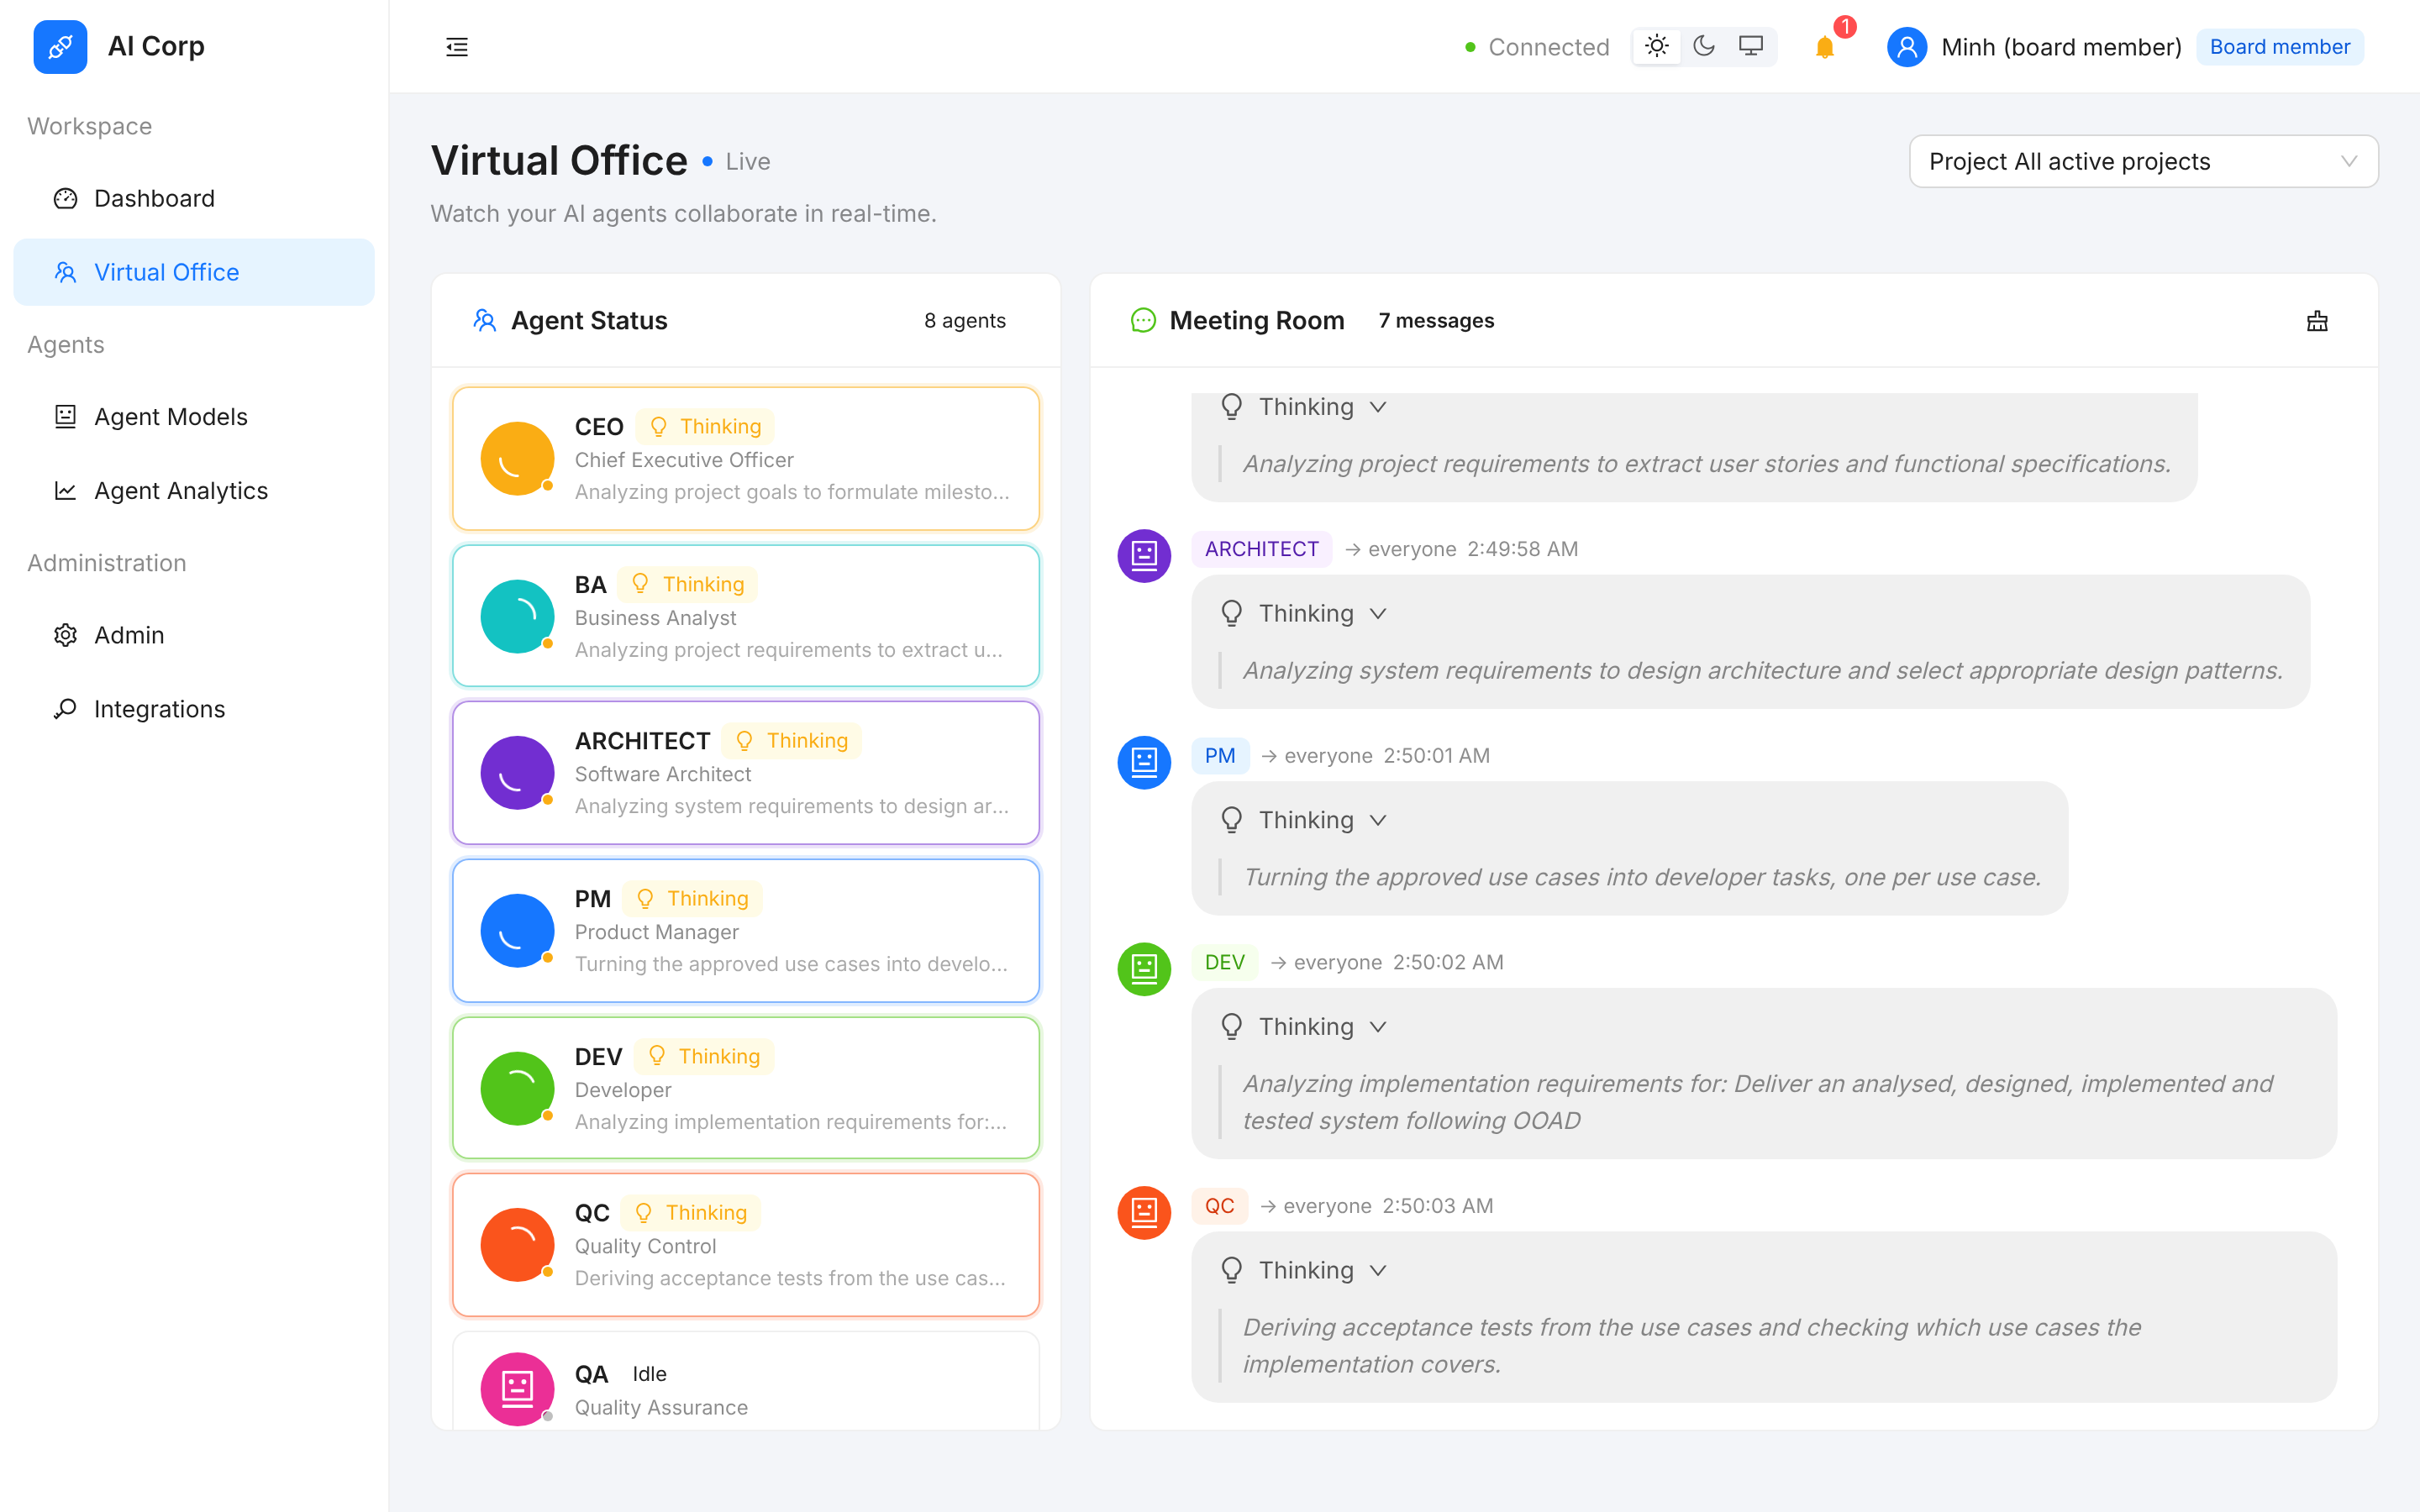
\includegraphics[width=\textwidth]{anh/meeting-room.png}
\end{figure}

\section{Thiết kế bộ máy quy trình}
\label{sec:bo-may}

\subsection{Định nghĩa và thực thi}

Một quy trình là một đồ thị gồm các nút có kiểu và các cạnh. Cạnh có thể là cạnh mặc định, cạnh có điều kiện hoặc cạnh \code{onFail}. \code{WorkflowEngine} không chứa logic riêng của loại nút nào. Mỗi loại nút là một \code{NodeExecutionStrategy} tự đăng ký vào bộ máy (Hình~\ref{fig:lop-bo-may}). Muốn thêm loại nút mới, chẳng hạn cổng chất lượng, chỉ cần viết thêm một lớp mà không phải sửa vòng lặp thực thi. Đó chính là nguyên lý OCP.

\begin{figure}{Sơ đồ lớp của bộ máy quy trình}
\label{fig:lop-bo-may}
\centering
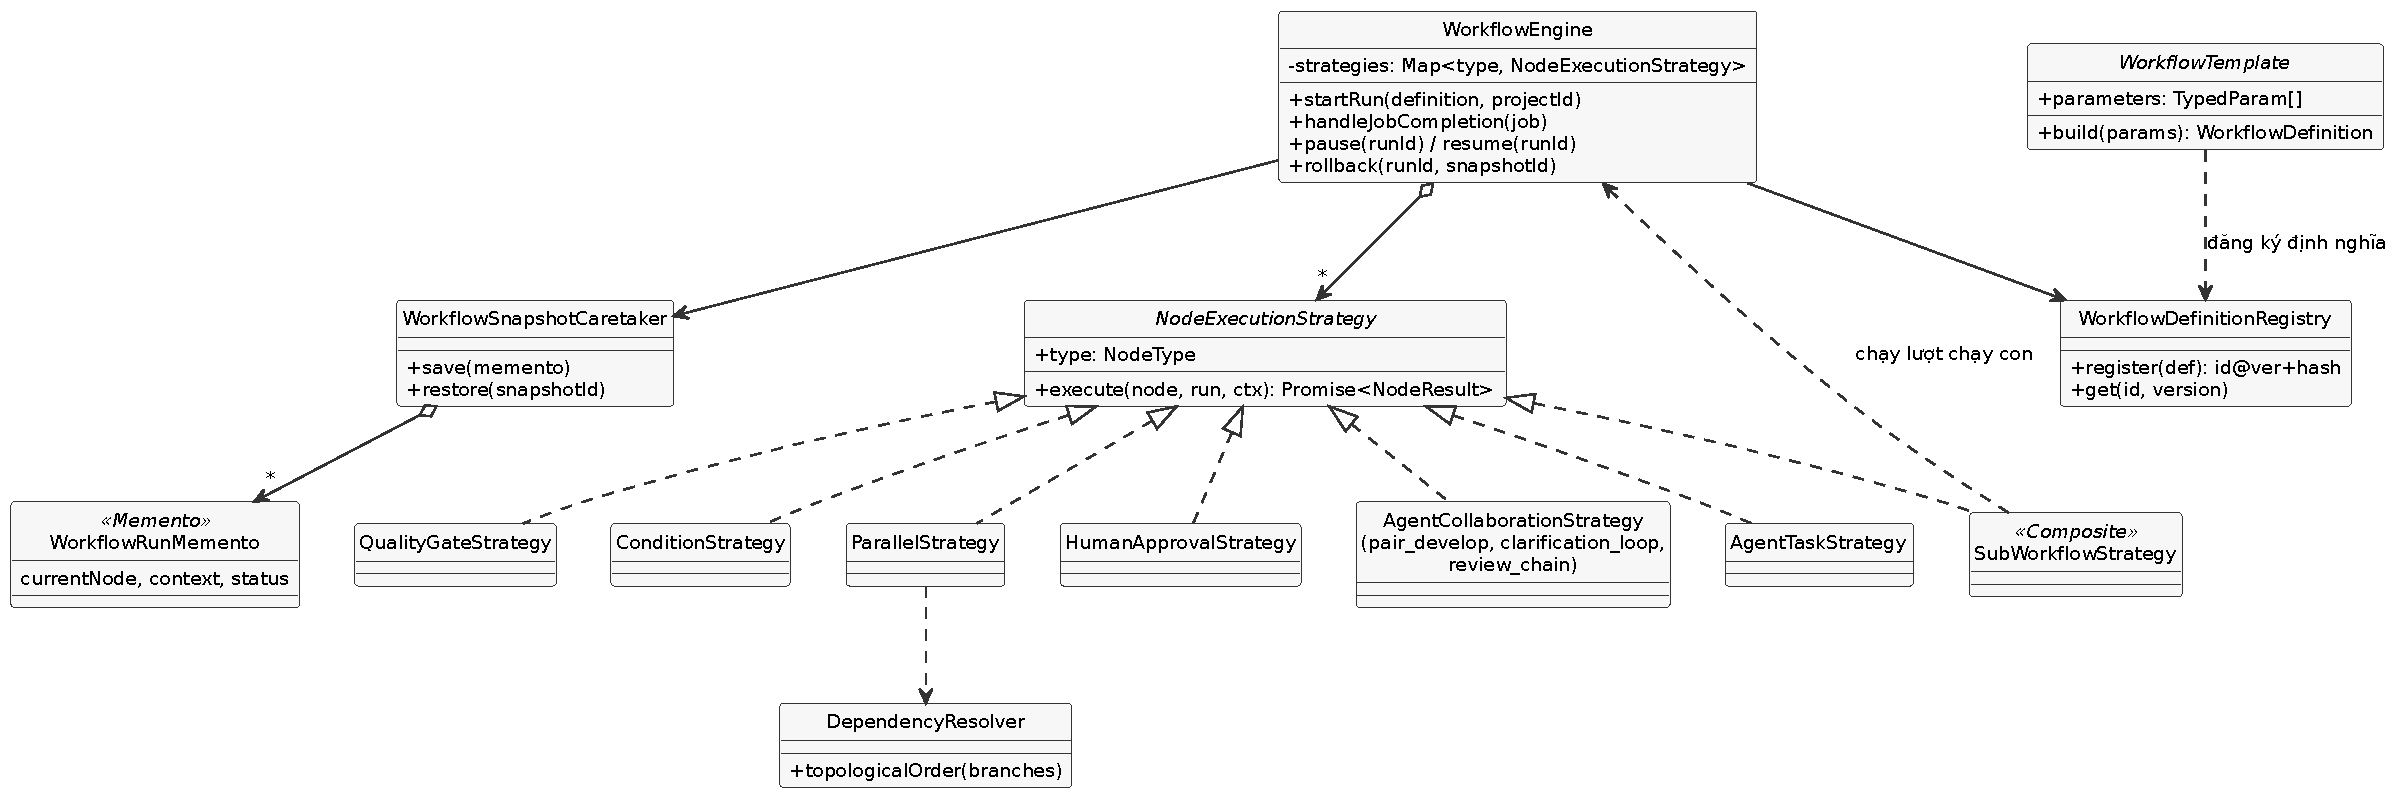
\includegraphics[width=\textwidth]{sodo/lop-bo-may-quy-trinh.pdf}
\end{figure}

Hình~\ref{fig:quy-trinh} là quy trình mặc định cho một dự án phần mềm. Quy trình này có hai quy trình con, mỗi cái có một vòng lặp. Vòng thiết kế quay lại Architect khi cổng OOAD không đạt, còn vòng xây dựng quay lại DEV khi QA từ chối.

\begin{figure}{Quy trình mặc định của một dự án phần mềm OOAD}
\label{fig:quy-trinh}
\centering
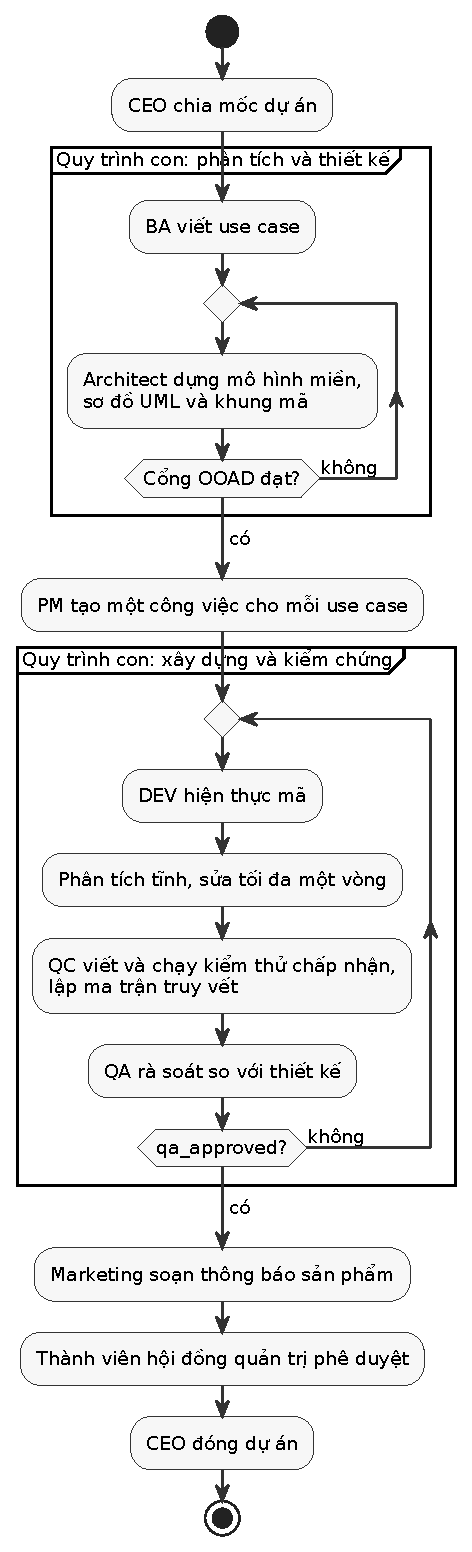
\includegraphics[height=0.62\textheight]{sodo/quy-trinh-mac-dinh.pdf}
\end{figure}

Hình~\ref{fig:tuan-tu-nut} cho thấy một nút tác tử đi qua những lớp nào. Bộ máy kiểm tra ngân sách trước, đẩy công việc vào hàng đợi, chiến lược nút gọi tác tử, tác tử gọi LLM qua Facade và Decorator. Khi nút xong, bộ máy ghi bước, chụp memento và chọn cạnh kế tiếp.

\begin{figure}{Tuần tự xử lý một nút tác tử}
\label{fig:tuan-tu-nut}
\centering
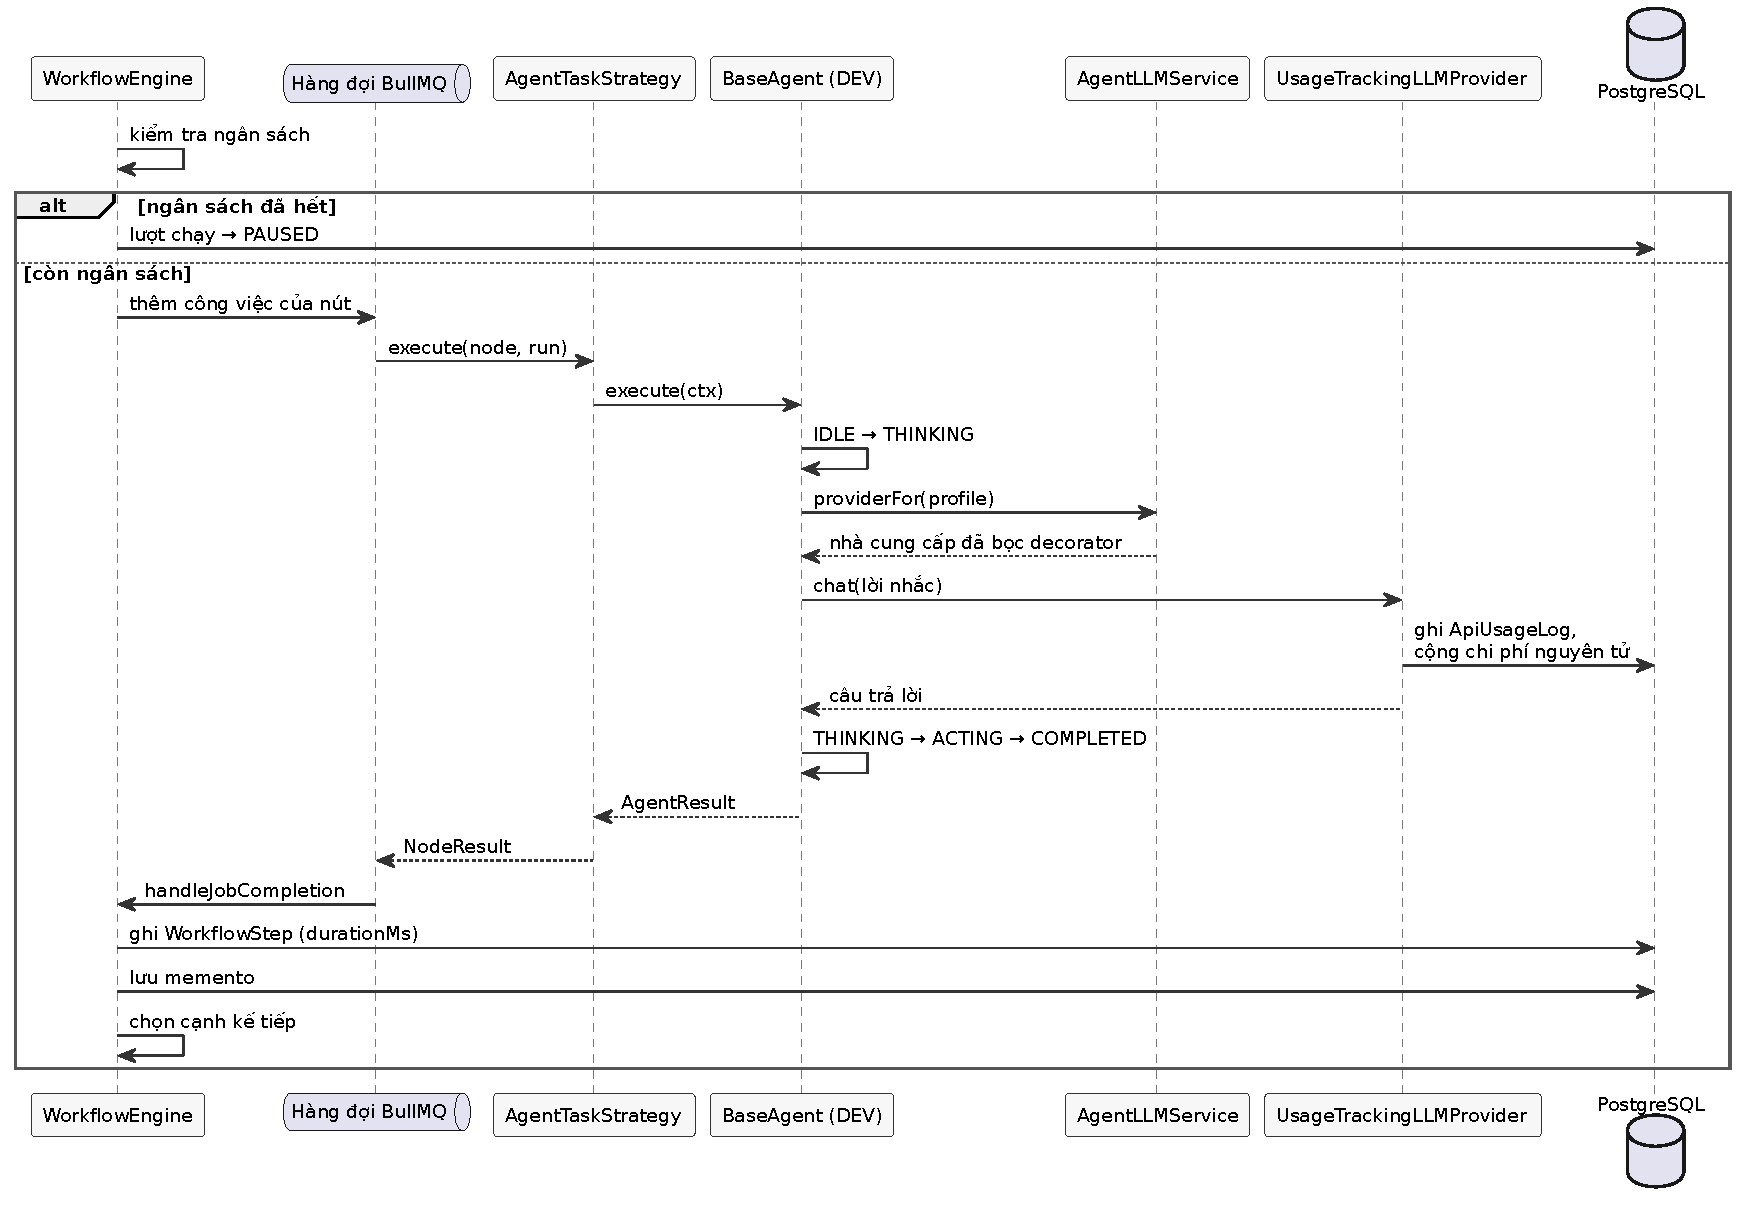
\includegraphics[width=\textwidth]{sodo/tuan-tu-thuc-thi-nut.pdf}
\end{figure}

\subsection{Quy trình con, phiên bản và khôi phục}

\begin{itemize}
\item \textbf{Quy trình con (Composite).} Nút \code{sub_workflow} chạy một quy trình khác thành lượt chạy con có \code{parentRunId}. Kết quả của lượt chạy con được gộp vào ngữ cảnh của lượt chạy cha. Ba mẫu quy trình có kiểu (dự án phần mềm OOAD, backend REST API, chỉ phân tích và thiết kế) dùng chung các quy trình con này.
\item \textbf{Phiên bản bất biến.} Mỗi định nghĩa quy trình được lưu theo khoá \code{id@phiên_bản} cùng mã băm của nội dung đã chuẩn hoá. Đăng ký lại cùng phiên bản với nội dung khác sẽ bị từ chối, và mỗi lượt chạy gắn cố định với một phiên bản.
\item \textbf{Ảnh chụp và khôi phục (Memento).} Sau mỗi nút, \code{WorkflowSnapshotCaretaker} lưu một memento gồm nút hiện tại, ngữ cảnh và trạng thái. Người dùng có thể đưa một lượt chạy đang tạm dừng về một ảnh chụp trước đó. Khi ấy các yêu cầu phê duyệt còn treo phát sinh sau ảnh chụp sẽ bị huỷ.
\item \textbf{Song song có phụ thuộc.} Nút \code{parallel} chạy các nhánh theo thứ tự tô-pô xác định bởi \code{dependsOn}, có giới hạn số nhánh chạy cùng lúc. \code{DependencyResolver} lo việc phát hiện chu trình phụ thuộc.
\end{itemize}

\subsection{Xử lý lỗi}

Nút lỗi được thử lại tối đa ba lần, mỗi lần chờ lâu gấp đôi lần trước. Vẫn lỗi thì lượt chạy đi theo cạnh \code{onFail} nếu có, còn không thì chuyển sang \code{failed} và phát \code{workflow.failed}. Kiểm thử đã lôi ra hai lỗi thiết kế ở đúng chỗ này. Trước khi sửa, một nút lỗi có thể làm lượt chạy kẹt mãi ở \code{running}, hoặc ngược lại cho lượt chạy đi tiếp theo cạnh thành công như chưa hề có lỗi.

\subsection{Điều khiển lượt chạy và ngân sách}

Các thao tác tạm dừng, tiếp tục và huỷ tác động lên lượt chạy mới nhất của dự án chứ không chỉ đổi trạng thái dự án. Xoá dự án thì lượt chạy bị huỷ và kho tệp cũng bị xoá theo. Có ba quy tắc giữ cho các thao tác này chạy đúng:

\begin{itemize}
\item Không cho tiếp tục khi lượt chạy đang chờ phê duyệt, vì nút phê duyệt sẽ chạy lại và sinh ra yêu cầu phê duyệt thứ hai. Cũng không cho tiếp tục khi ngân sách đã hết. Cả hai trường hợp đều trả lỗi kèm lý do.
\item Không nút nào được bắt đầu khi ngân sách đã hết. Bộ máy kiểm tra ngân sách trước mỗi nút và tạm dừng lượt chạy nếu cần. Chi phí được cộng bằng phép tăng nguyên tử trong cơ sở dữ liệu thay cho kiểu đọc rồi ghi. Thông báo ở mức 90\% và 100\% chỉ phát một lần, đúng lúc vượt ngưỡng.
\item Nút nào đã chạy xong trong lúc lượt chạy bị tạm dừng thì không chạy lại khi tiếp tục.
\end{itemize}

Ba quy tắc này có được sau đợt rà soát mã giao diện và logic. Trước đó, nút \textit{Pause} trên giao diện chỉ đổi trạng thái dự án trong khi lượt chạy vẫn chạy tiếp, còn ngân sách chỉ được kiểm tra sau khi tiền đã tiêu. Hình~\ref{fig:sm-luot-chay} tổng hợp các trạng thái của lượt chạy sau khi sửa.

\begin{figure}{Máy trạng thái của lượt chạy quy trình}
\label{fig:sm-luot-chay}
\centering
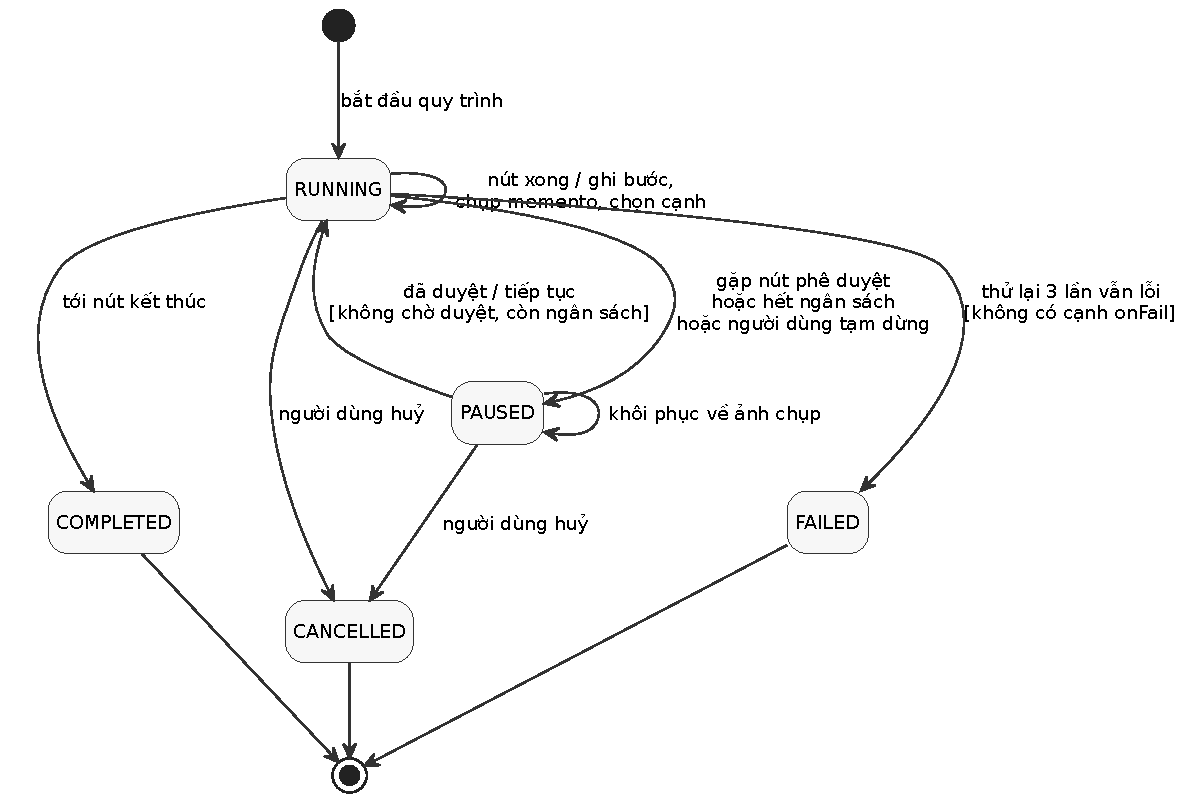
\includegraphics[width=0.8\textwidth]{sodo/may-trang-thai-luot-chay.pdf}
\end{figure}

\section{Thiết kế dữ liệu và lưu trữ}

Dữ liệu có cấu trúc nằm trong PostgreSQL qua 22 mô hình Prisma: người dùng, dự án, mốc, công việc, tác tử, bộ nhớ, lượt chạy, bước, ảnh chụp, phiên bản định nghĩa, phê duyệt, nhật ký sử dụng API, nhật ký cổng chất lượng, nhật ký kiểm toán, khoá API, webhook, lần gửi webhook, dự báo, nhà cung cấp LLM, mô hình LLM và một số bảng khác. Lược đồ được quản lý bằng migration có phiên bản. Một bước kiểm tra riêng so lược đồ dựng từ migration với mô hình Prisma để bắt sai lệch.

Sản phẩm của tác tử (tài liệu, sơ đồ, mã, kiểm thử, báo cáo) không nằm trong cơ sở dữ liệu mà nằm trong \code{ProjectWorkspace}, một thư mục lâu dài cho mỗi dự án. Mọi đường dẫn ghi vào đều được kiểm tra để không thoát ra ngoài thư mục đó, nên một đường dẫn kiểu \code{../../etc/...} do LLM đề xuất sẽ bị từ chối. Ở thiết kế cũ, sản phẩm được ghi vào sandbox Docker, mà sandbox chạy mỗi lệnh trong một container mới không gắn ổ đĩa, nên tệp mất ngay sau mỗi lệnh. Cũng vì vậy mà cổng chất lượng và bước quét kiểm thử của bản cũ chưa lần nào chạy được.

\section{Áp dụng OOAD cho dự án sinh ra}
\label{sec:ooad-du-an}

Dự án nào do nền tảng sinh ra cũng đi qua cùng một chuỗi OOAD, và mắt xích nào trong chuỗi cũng được kiểm tra tự động (Hình~\ref{fig:chuoi-ooad}).

\subsection{Chuỗi sản phẩm}

Bảng~\ref{tab:chuoi-sp} liệt kê sản phẩm của từng bước. Khung mã được dựng từ các mẫu Handlebars theo đúng bốn tầng. Giao diện Repository nằm ở tầng miền, phần hiện thực nằm ở tầng hạ tầng, còn tệp \code{composition-root.ts} ráp các phụ thuộc lại với nhau. Nói cách khác, nền tảng đòi hỏi ở sản phẩm đúng cái kiến trúc mà nó tự áp cho mình.

\begin{table}{Chuỗi sản phẩm OOAD của một dự án sinh ra}
\label{tab:chuoi-sp}
\small
\begin{tabularx}{\textwidth}{|P{2.6cm}|P{2cm}|L|}
\hline
\textbf{Bước} & \textbf{Thực hiện} & \textbf{Sản phẩm trong kho tệp dự án} \\ \hline
Yêu cầu & BA & \code{docs/use-cases.md} \\ \hline
Mô hình miền và UML & Architect & \code{docs/domain-model.puml}, \code{docs/use-case-diagram.puml}, \code{docs/class-diagram.puml}, \code{docs/sequence-UC-xxx.puml}, \code{docs/architecture-patterns.md}, \code{ARCHITECTURE.md} \\ \hline
Khung mã & Architect & \texttt{src/domain/\{entities, value-objects, repositories\}}, \code{src/application/services}, \code{src/infrastructure/persistence}, \code{src/presentation/controllers}, \code{src/composition-root.ts} \\ \hline
Hiện thực & DEV & Mã đầy đủ trong khung, có chú thích \code{UC-xxx} \\ \hline
Chất lượng mã & Hệ thống & \code{docs/code-quality.md} \\ \hline
Kiểm thử & QC & \code{tests/UC-xxx.spec.ts}, kết quả Jest \\ \hline
Truy vết & QC & \code{docs/traceability-matrix.md} \\ \hline
\end{tabularx}
\end{table}

\begin{figure}{Chuỗi OOAD của dự án sinh ra và ba lớp kiểm tra}
\label{fig:chuoi-ooad}
\centering
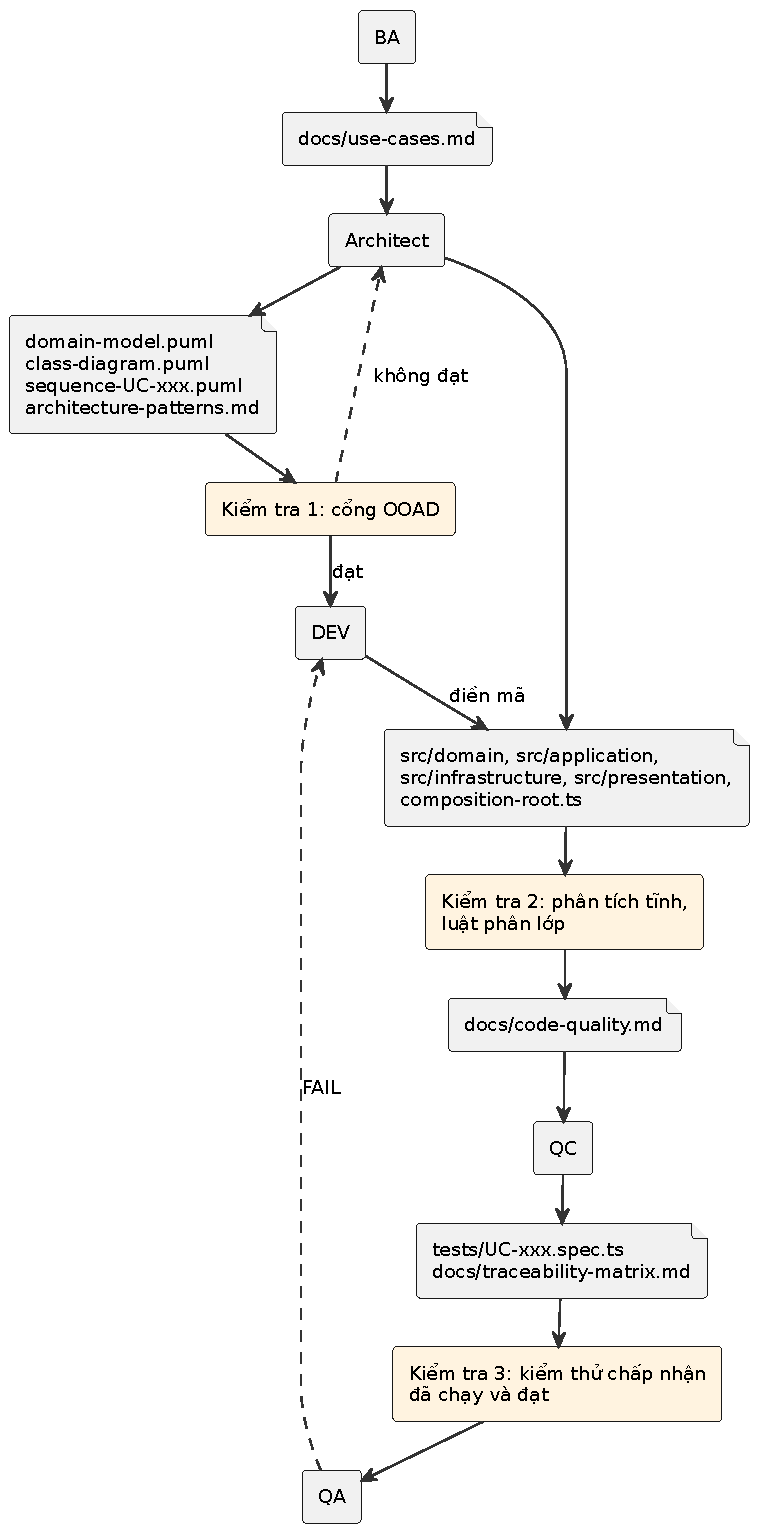
\includegraphics[height=0.6\textheight]{sodo/chuoi-ooad-du-an.pdf}
\end{figure}

\subsection{Ba lớp kiểm tra}

\begin{enumerate}
\item \textbf{Cổng OOAD.} Nút \code{quality_gate} đặt sau bước thiết kế, kiểm tra xem số use case, số thực thể miền, số mẫu thiết kế có đủ ngưỡng không và các tệp bắt buộc đã có chưa. Không đạt thì quy trình quay lại Architect. Mỗi lần đánh giá được ghi vào \code{QualityGateLog} và phát \code{QualityGateEvaluatedEvent}.
\item \textbf{Phân tích tĩnh trước khi QA rà soát} (mục~\ref{subsec:phan-tich-tinh}). Trong đó có luật phân lớp \textit{miền ← ứng dụng ← hạ tầng, trình bày}, theo đó mọi lệnh \code{import} hoặc \code{require()} từ tầng miền sang tầng hạ tầng đều tính là vi phạm.
\item \textbf{Kiểm thử chấp nhận đã chạy.} Độ bao phủ use case chỉ tính những use case có kiểm thử đã chạy và đạt. Use case thiếu kiểm thử hoặc có kiểm thử hỏng được liệt kê đích danh.
\end{enumerate}

Hình~\ref{fig:artifacts} là tab \textit{Artifacts} của một dự án sinh ra. Ở đây người dùng xem được tóm tắt OOAD, kết quả cổng chất lượng, cây tệp, và mở từng sơ đồ đã render. Trong hình đang mở mô hình miền \code{docs/domain-model.puml}.

\begin{figure}{Tab Artifacts của dự án Online Bookstore}
\label{fig:artifacts}
\centering
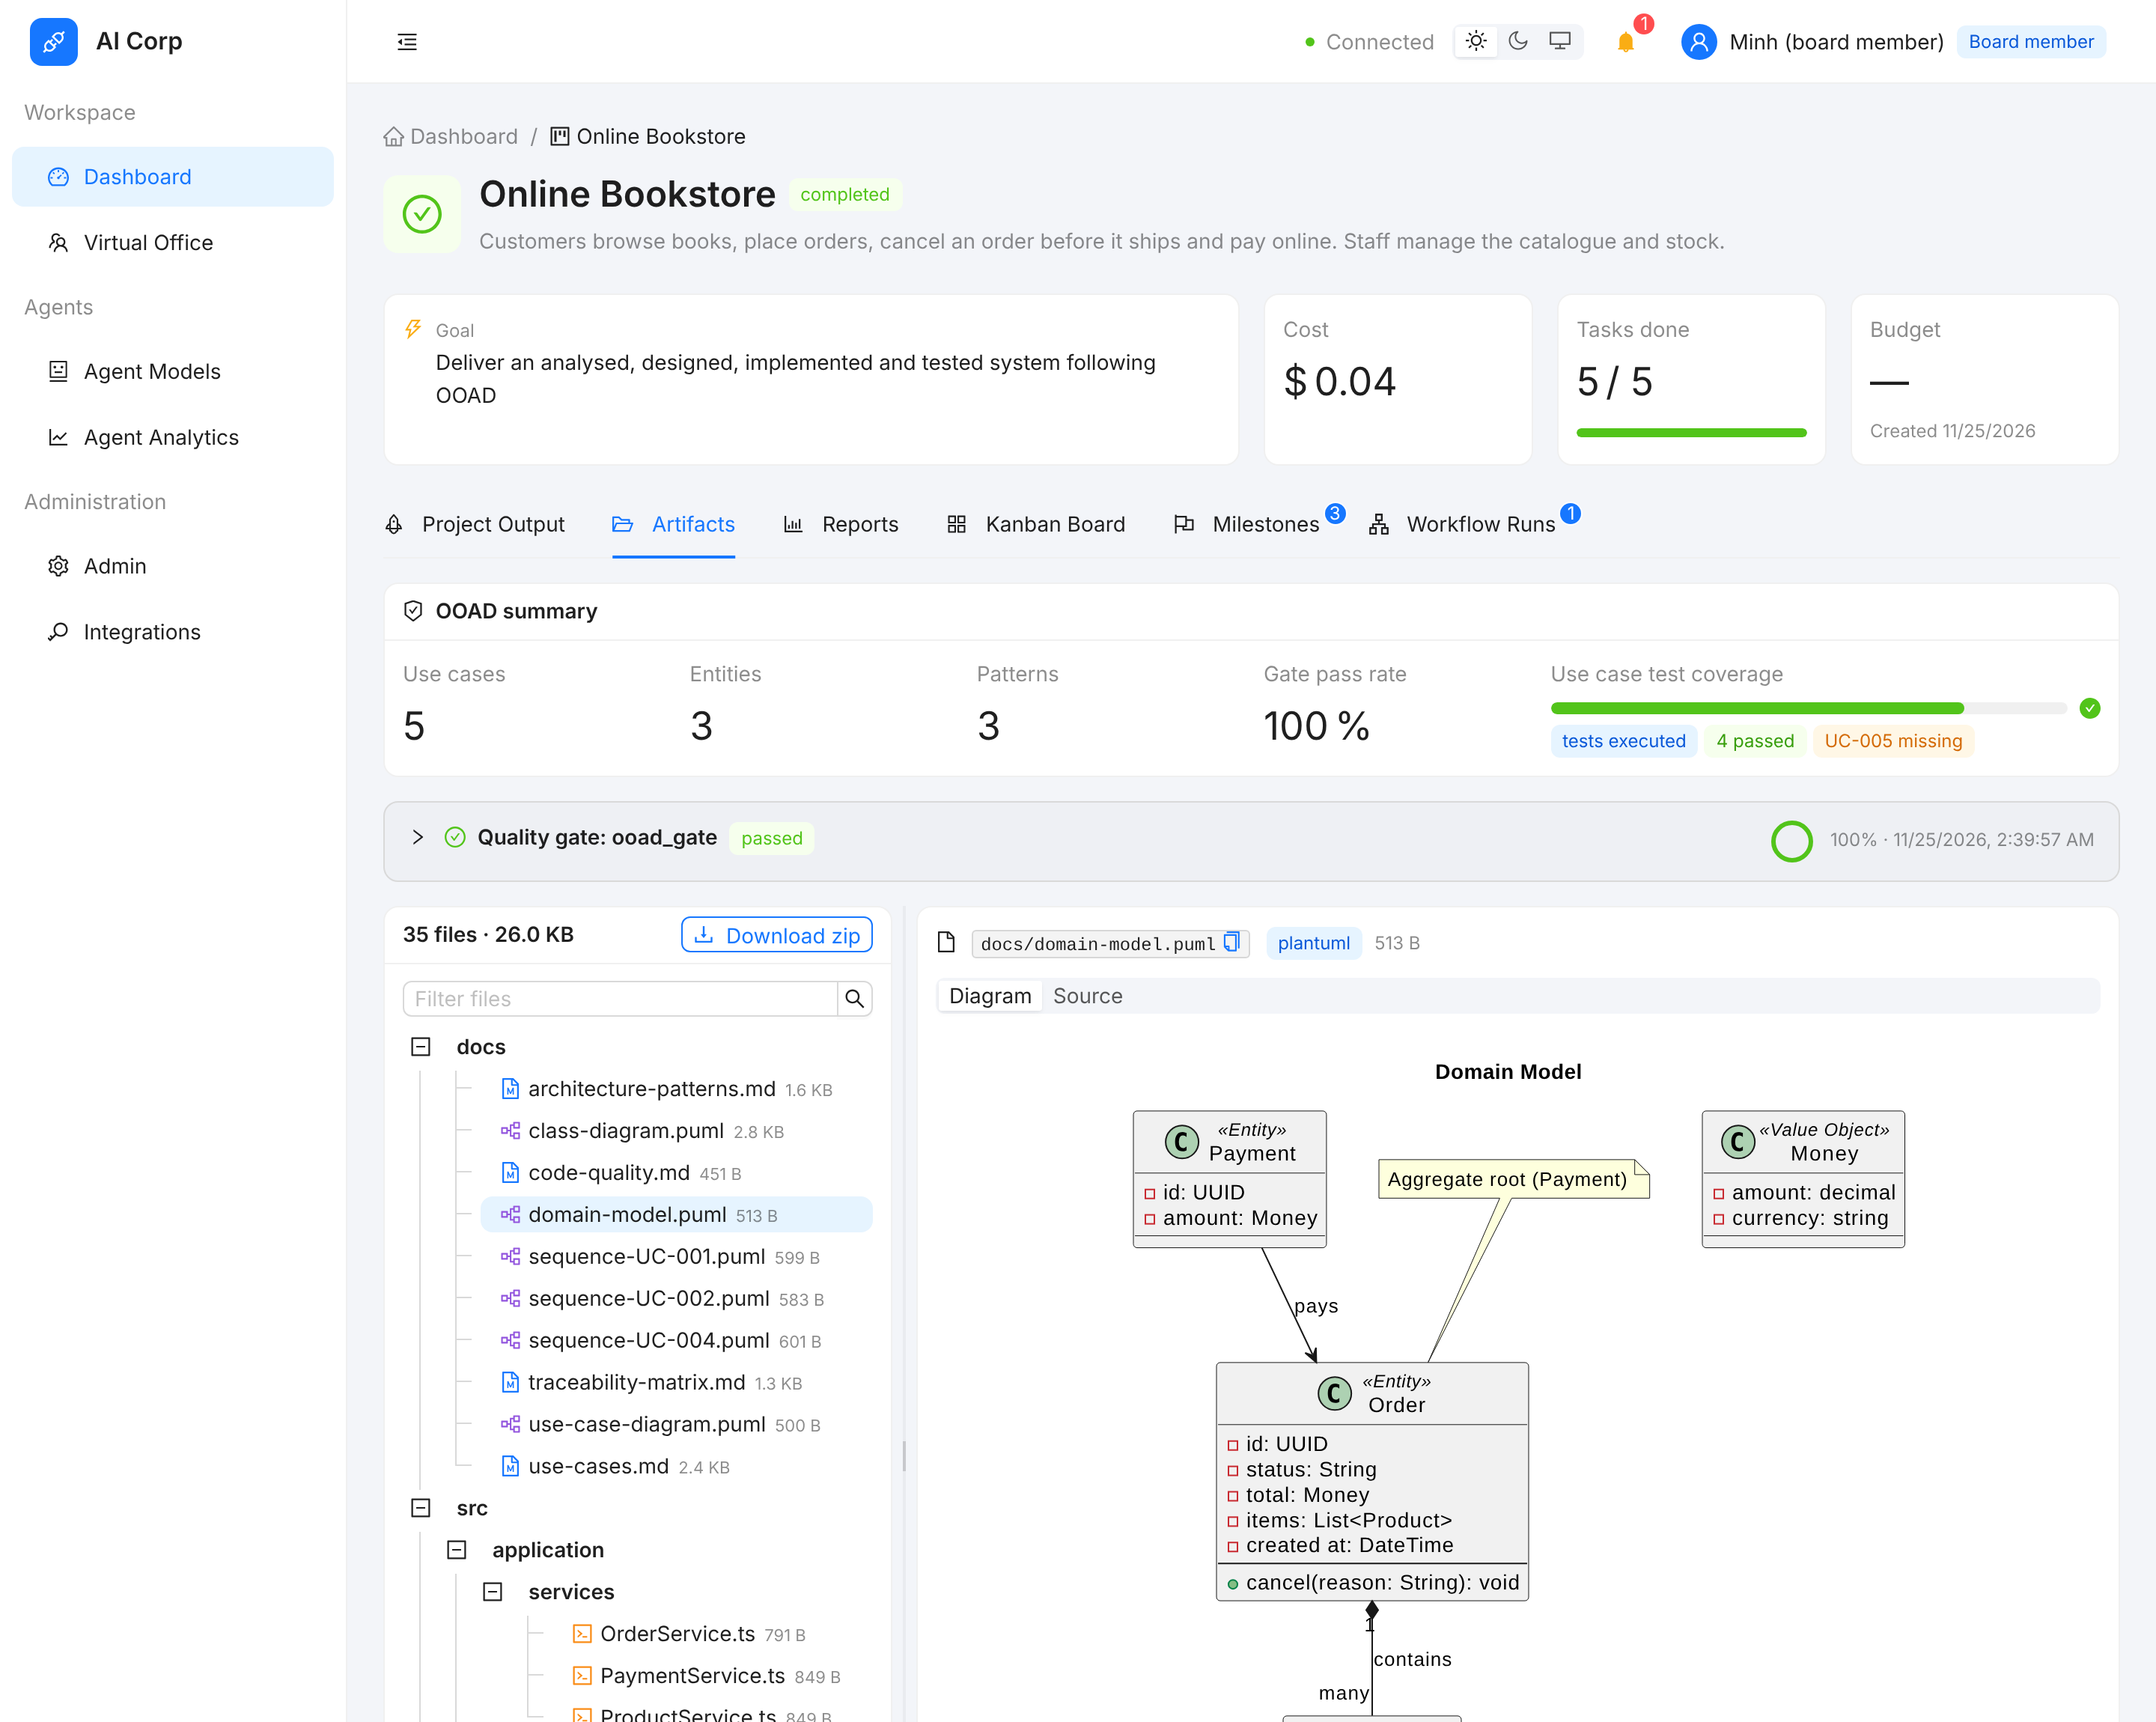
\includegraphics[width=\textwidth]{anh/artifacts.png}
\end{figure}

\section{Bảo mật và tính năng doanh nghiệp}

\begin{itemize}
\item \textbf{Chuỗi guard toàn cục} theo mẫu Chain of Responsibility (Hình~\ref{fig:guard}): \code{AuthenticationGuard} xác thực JWT~\cite{rfc7519} cho người dùng hoặc khoá API cho nhóm \code{/api/v1}, sau đó tới \code{RateLimitGuard}, rồi \code{PermissionGuard}. Mặc định route nào cũng phải đăng nhập, route công khai phải gắn \code{@Public} rõ ràng.
\item \textbf{Quyền của chủ dự án.} \code{AuthorizationService} kiểm tra chủ dự án và người được giao phê duyệt, sai thì trả 403 và ghi \code{access.denied}. Tạo và sửa công việc cũng kiểm tra quyền chủ dự án như khi sửa dự án.
\item \textbf{Đặc quyền tối thiểu khi đăng ký.} Tài khoản tự đăng ký chỉ nhận vai trò người xem (\code{SIGNUP_ROLE}). Quản trị viên nâng quyền ở trang quản lý người dùng và có thể tắt đăng ký (\code{ALLOW_REGISTRATION=false}). Phiên đăng nhập hết hạn sau \code{JWT_EXPIRATION}, mặc định 8 giờ.
\item \textbf{Nhật ký kiểm toán chỉ ghi thêm.} Decorator \code{@Audited} cùng \code{AuditInterceptor} ghi hành động của người dùng, còn \code{AuditLogHandler} ghi hành động của hệ thống và tác tử từ sự kiện miền. Mật khẩu, token, bí mật và khoá được che trước khi ghi.
\item \textbf{API tích hợp.} Khoá API chỉ mang những phạm vi mà vai trò hiện tại của chủ khoá cho phép, tức giao của hai tập phạm vi. Mỗi khoá có giới hạn tần suất riêng. Tài liệu OpenAPI nằm ở \code{/api/docs} và tắt được ở production.
\item \textbf{Webhook.} Payload được ký HMAC-SHA256~\cite{rfc2104} kèm dấu thời gian. URL trỏ vào mạng nội bộ bị từ chối, kể cả khi chỉ lộ ra sau bước phân giải DNS, để chống tấn công SSRF~\cite{owasp2021}. Gửi lại khi lỗi theo thời gian chờ tăng dần.
\item \textbf{Phê duyệt chỉ qua REST.} Quyết định phê duyệt chỉ đi qua \code{POST /api/approvals/:id/approve} hoặc \code{.../reject}, nơi có kiểm tra quyền, kiểm tra người được giao và ghi kiểm toán. Việc trả lời là một cập nhật có điều kiện trên trạng thái \code{pending}, nên hai câu trả lời cùng lúc không thể cùng thành công, và câu thứ hai nhận 409 (Hình~\ref{fig:tuan-tu-phe-duyet}). Quyết định và lý do, bắt buộc khi từ chối, được ghi vào biến của lượt chạy để các tác tử phía sau đọc được.
\item \textbf{Cấu hình production an toàn.} Khi \code{NODE_ENV=production}, API không khởi động nếu thiếu \code{JWT_SECRET} hoặc giá trị này ngắn hơn 32 ký tự, thiếu \code{CORS_ORIGIN}, hay còn giá trị giữ chỗ như \code{CHANGE_ME}. Mọi nơi đọc khoá JWT (REST, guard WebSocket, cổng WebSocket) dùng chung một hàm. Trước đây ba nơi có ba giá trị dự phòng khác nhau, nên khi quên đặt \code{JWT_SECRET}, kết nối thời gian thực luôn bị từ chối.
\end{itemize}

\begin{figure}{Chuỗi guard xử lý một yêu cầu HTTP}
\label{fig:guard}
\centering
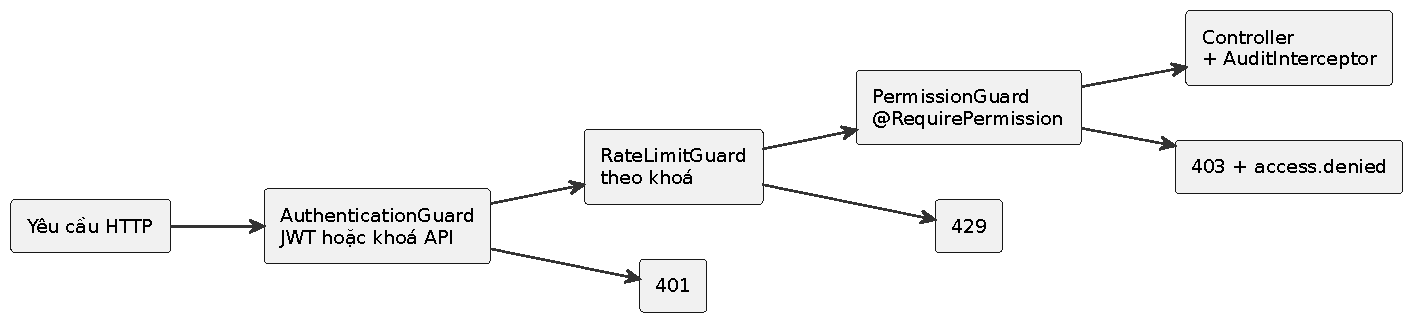
\includegraphics[width=0.9\textwidth]{sodo/chuoi-guard.pdf}
\end{figure}

\begin{figure}{Tuần tự phê duyệt một bước quy trình}
\label{fig:tuan-tu-phe-duyet}
\centering
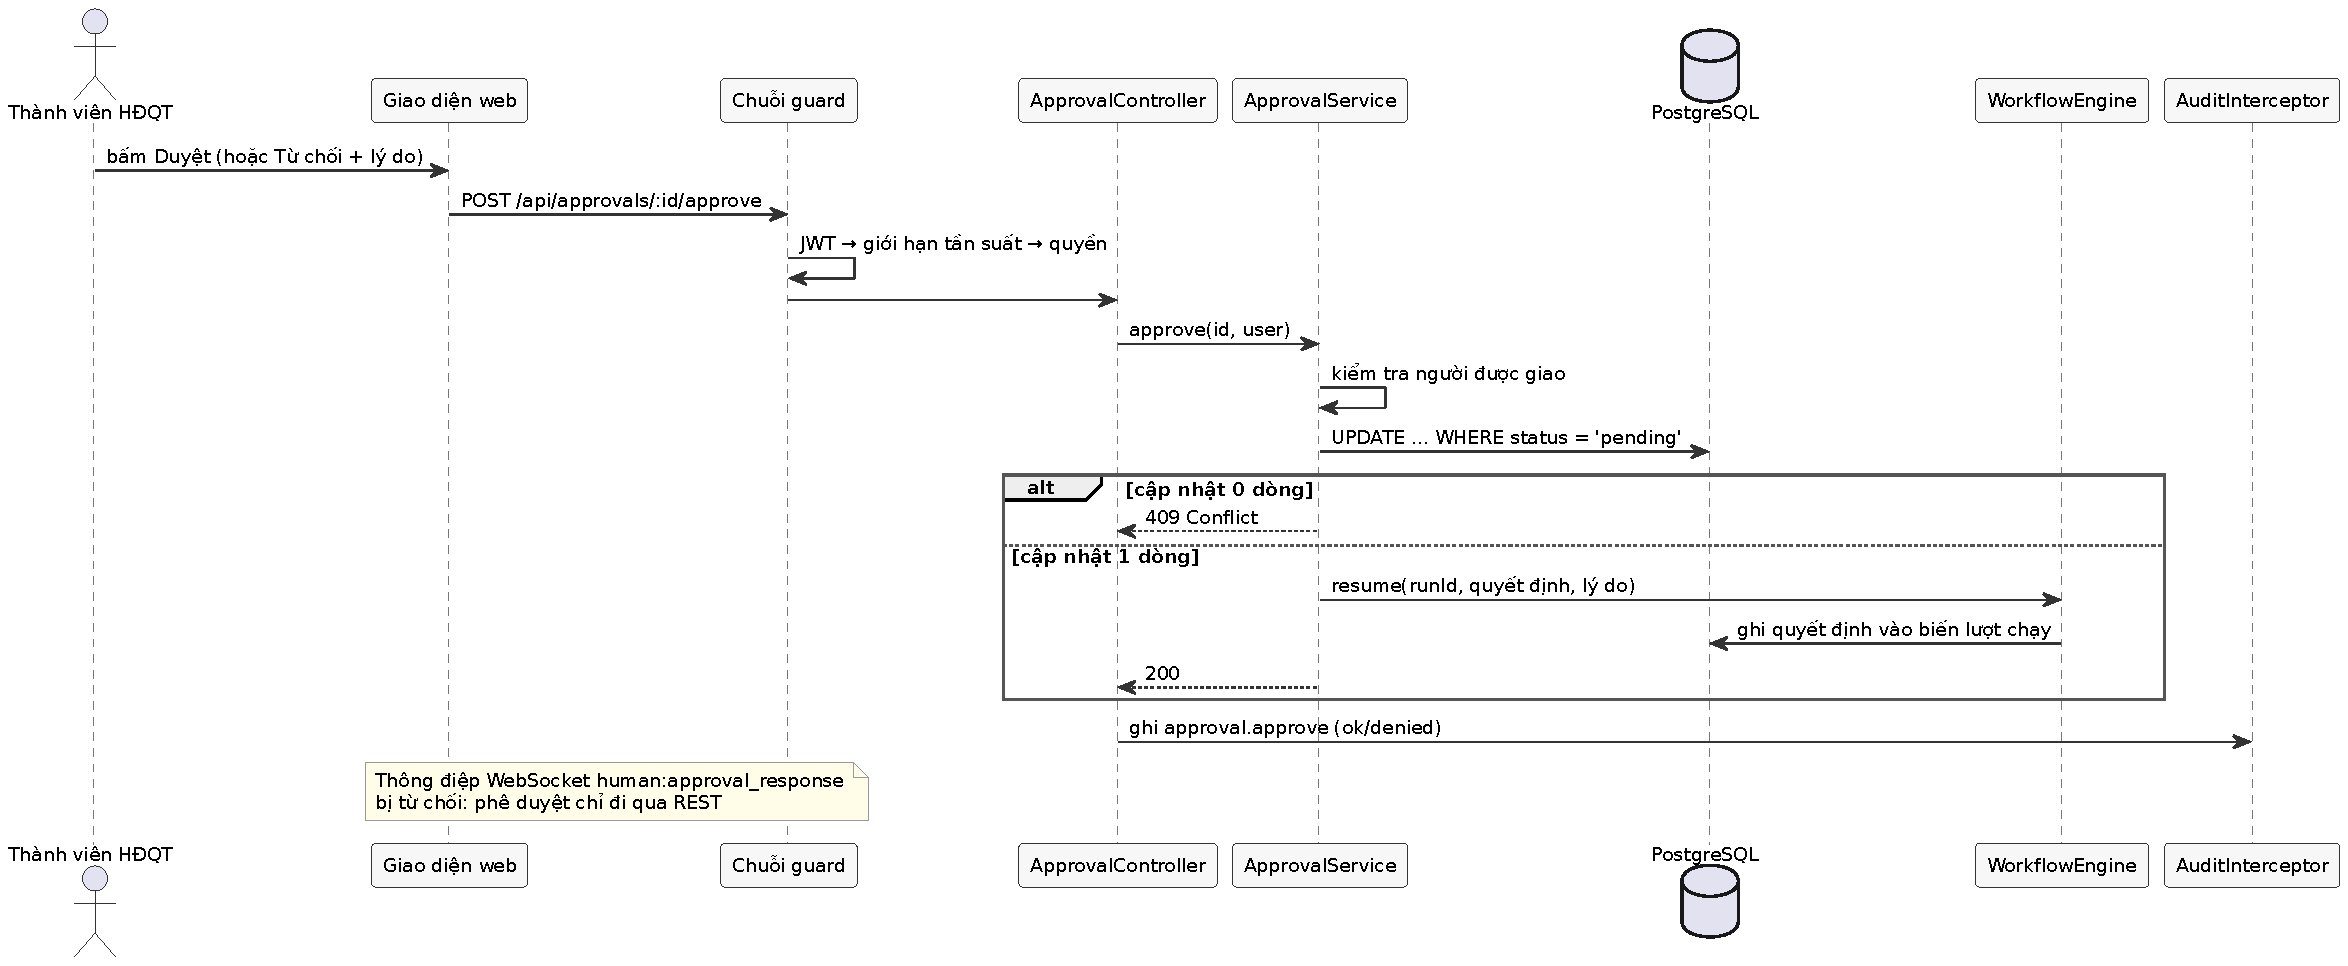
\includegraphics[width=\textwidth]{sodo/tuan-tu-phe-duyet.pdf}
\end{figure}

\section{Phân tích, dự báo và chất lượng mã}

\subsection{Phân tích hiệu năng tác tử}

\code{AgentPerformanceAnalyzer} là một hàm thuần ở tầng miền. Với mỗi vai trò, nó tính số bước, tỉ lệ thành công, thời lượng trung bình và phân vị 95, chi phí cho mỗi lần thành công, điểm chất lượng, xu hướng so với kỳ trước và thứ hạng. Điểm chất lượng không dùng chung một công thức mà đo theo tiêu chí hợp với từng vai trò, qua các \code{IQualitySignal}. DEV tính theo tỉ lệ được QA duyệt, QC theo kết quả kiểm thử, Architect theo kết quả cổng OOAD, các vai trò còn lại theo tỉ lệ đạt ngay lần đầu.

\code{AgentAnomalyDetector} áp năm quy tắc phát hiện bất thường: tỉ lệ thành công giảm 20 điểm phần trăm, ba lần thất bại liên tiếp, chi phí tăng gấp đôi, thời gian chạy tăng gấp đôi và chất lượng dưới 50\%. Mỗi bất thường phát tối đa một lần mỗi ngày qua cùng kênh sự kiện, kiểm toán và webhook.

\subsection{Dự báo thời gian và chi phí}

Nền tảng không chấm giờ công của con người mà ghi thời lượng và chi phí LLM của từng bước tác tử. Do đó mô hình dự báo nhắm vào thời gian của tác tử và chi phí LLM theo từng dự án, từng vai trò, chứ không dự báo giờ công cho từng công việc. Mỗi vai trò có một mô hình hồi quy ridge~\cite{hoerl1970} trên hai đặc trưng là độ dài mô tả dự án và số use case. Vai trò nào có dưới 6 mẫu thì dùng giá trị trung vị. Độ chính xác được báo bằng sai số leave-one-out (MAPE và MAE)~\cite{kohavi1995}, và mỗi dự báo đi kèm một mức tin cậy.

Dự báo được lưu hai lần, một lần khi quy trình bắt đầu và một lần khi PM lập kế hoạch. Xong dự án thì đem so với số liệu thật. Chi phí ước lượng của mỗi công việc PM tạo ra được suy từ dự báo của DEV, QC và QA.

\subsection{Phân tích tĩnh và vòng sửa có giới hạn}
\label{subsec:phan-tich-tinh}

\code{TypeScriptCodeAnalyzer} nằm ở tầng hạ tầng, phía sau cổng \code{ICodeAnalyzer}. Bộ phân tích dùng TypeScript compiler API để tìm lỗi cú pháp. Nó tính độ phức tạp McCabe của từng hàm~\cite{mccabe1976}, thể tích Halstead~\cite{halstead1977} và chỉ số bảo trì đã chuẩn hoá~\cite{oman1992,coleman1994}. Nó cũng tìm lời gọi nguy hiểm như \code{eval} hay \code{Function}, bí mật viết cứng trong mã, vi phạm phân lớp, và gom các chỗ tham chiếu tới use case.

\code{CodeQualityPolicy} ở tầng miền trừ điểm cho từng loại vấn đề, mỗi loại có mức trừ tối đa, rồi lấy trung bình có trọng số theo số dòng. Chính sách dự đoán QA sẽ trả \textit{fail} khi điểm dưới 70, khi có lỗi cú pháp hoặc khi có vi phạm phân lớp. Nếu dự đoán là \textit{fail}, DEV được sửa đúng một vòng, có kèm danh sách vấn đề, và bản sửa chỉ được giữ khi điểm tăng. Khi rà soát, QA dùng báo cáo phân tích làm bằng chứng. Về sau dự đoán này được đem so với phán quyết thật để đo độ chính xác.

\section{Thiết kế triển khai}

Hệ thống được triển khai bằng Docker Compose trên một máy chủ (Hình~\ref{fig:trien-khai}). nginx phục vụ ứng dụng web và làm proxy ngược cho \code{/api}, \code{/socket.io}, \code{/plantuml}. API chạy trên Node~20, khởi động thì chạy migration trước rồi mới nhận yêu cầu. Ngoài ra còn có PostgreSQL kèm pgvector, Redis ở chế độ AOF và một máy chủ PlantUML nội bộ. Kho tệp các dự án là một volume. Chỉ nginx mở cổng ra ngoài. Hồ sơ \code{demo} chạy kèm LLM kịch bản để trình diễn khi không có mạng.

API có hai điểm kiểm tra tình trạng (health check) theo gợi ý của Nygard~\cite{nygard2018}. \code{/api/health/live} cho biết tiến trình còn sống và được Docker dùng làm HEALTHCHECK. \code{/api/health} cho biết hệ thống đã sẵn sàng phục vụ hay chưa. Nó trả 503 khi mất kết nối cơ sở dữ liệu và trả trạng thái \textit{degraded} khi mất Redis hoặc cổng LLM.

\begin{figure}{Sơ đồ triển khai}
\label{fig:trien-khai}
\centering
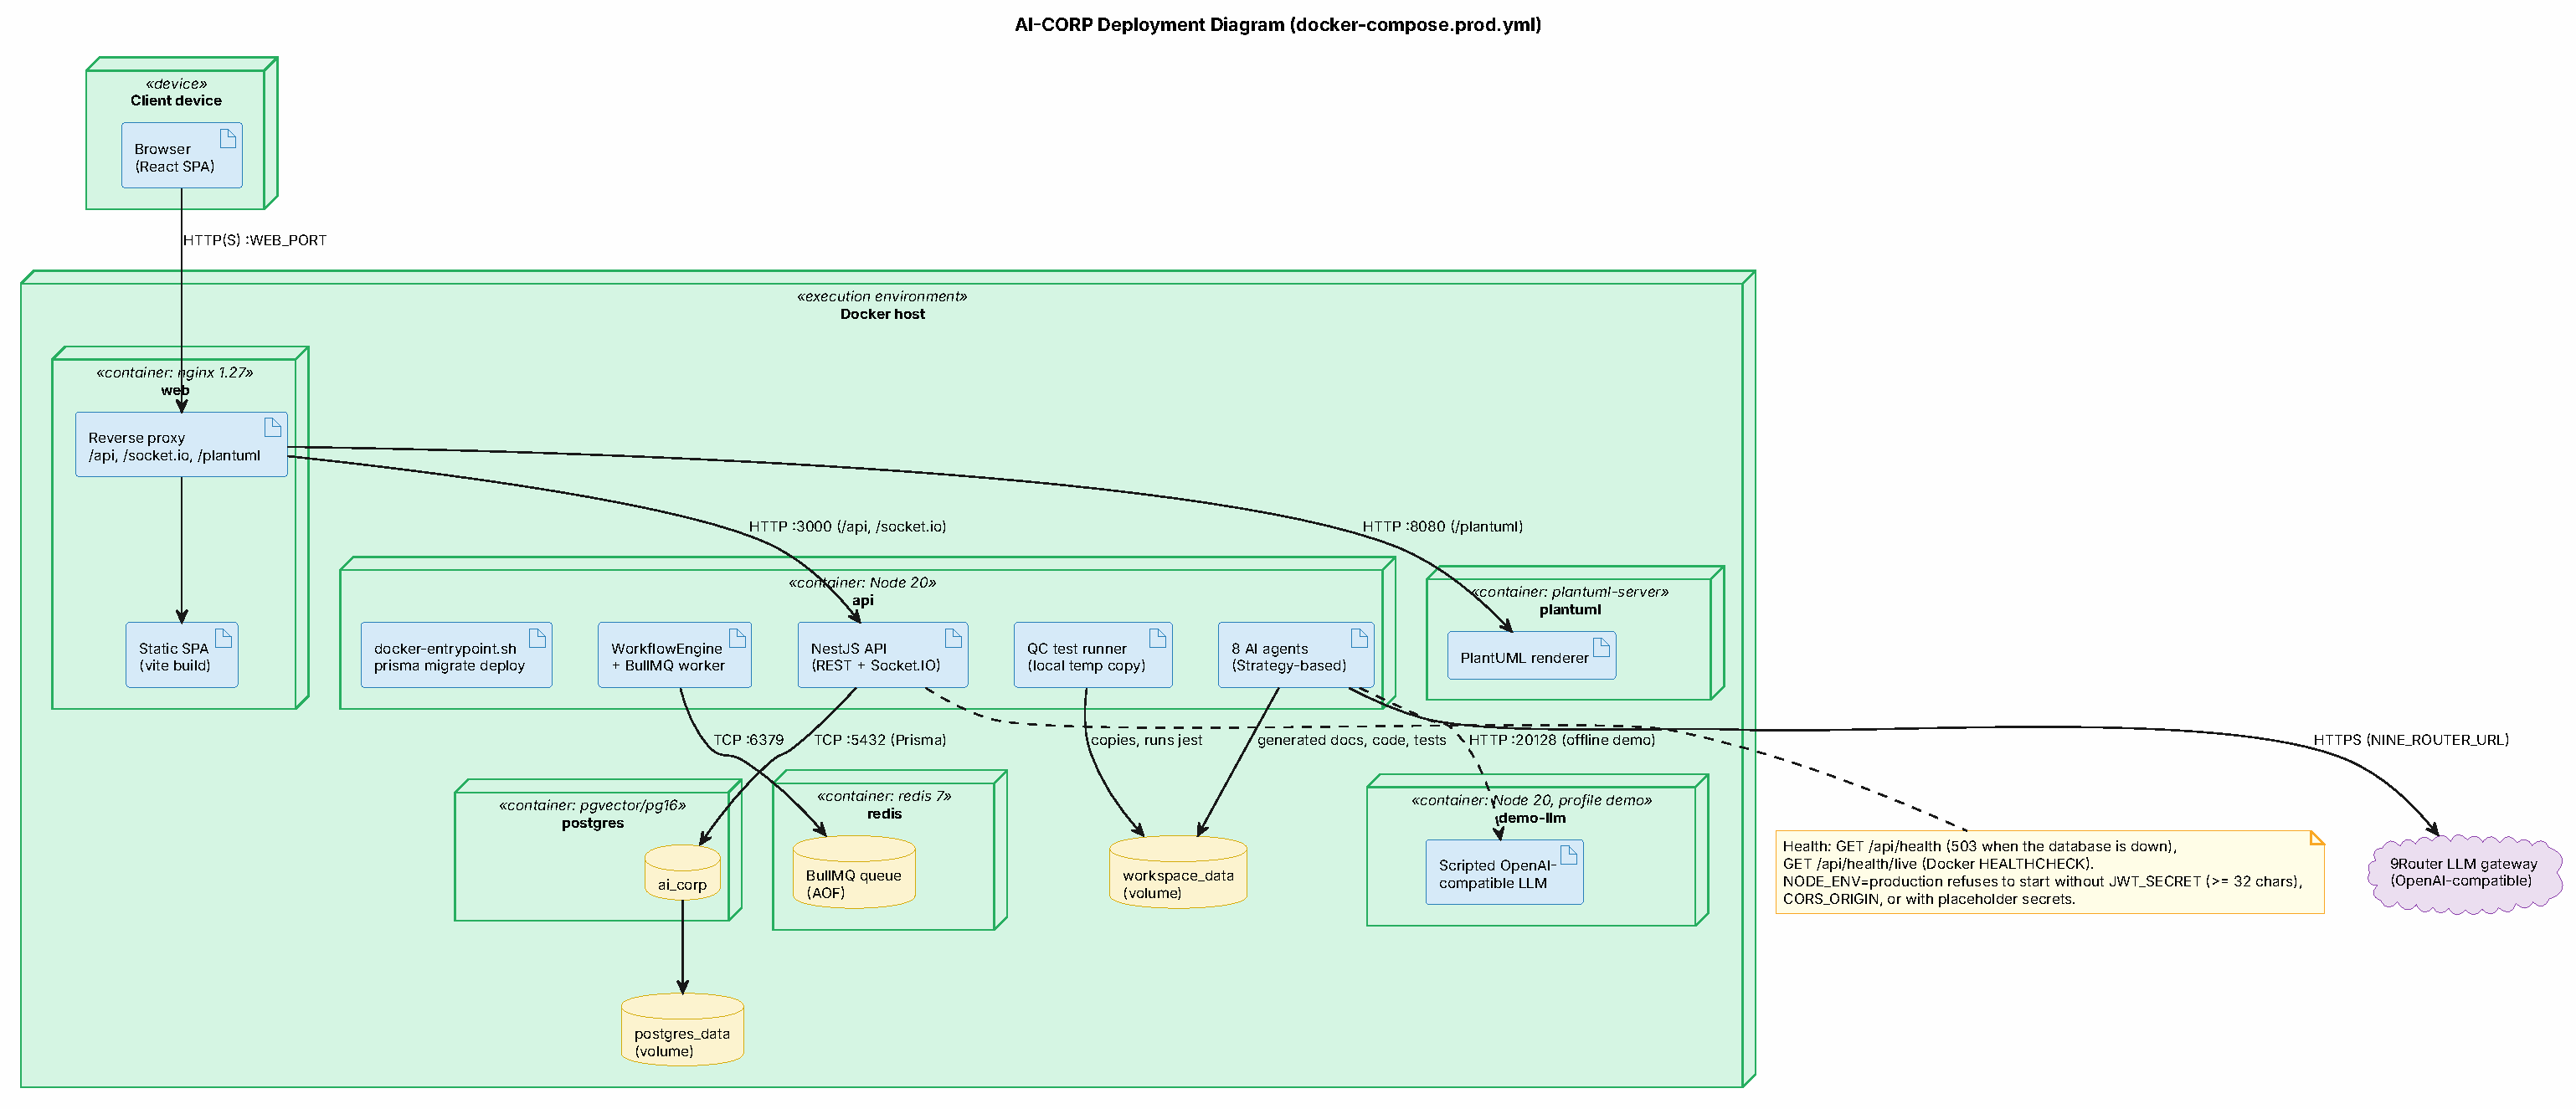
\includegraphics[width=\textwidth]{uml/deployment-diagram.pdf}
\end{figure}

\chapter{Hiện thực hệ thống}
\label{chap:hien-thuc}

Chương này kể lại thiết kế ở chương~\ref{chap:thiet-ke} đã thành mã như thế nào. Lần lượt là công nghệ dùng, quy mô mã nguồn, vài đoạn mã tiêu biểu cho các mẫu thiết kế chính, giao diện người dùng và cấu hình triển khai.

\section{Công nghệ và quy mô mã nguồn}

Bảng~\ref{tab:cong-nghe} liệt kê công nghệ của từng thành phần. Toàn bộ mã nằm trong một monorepo, quản lý bằng pnpm và Turborepo, gồm ba gói: \code{apps/api}, \code{apps/web} và \code{packages/shared-types}. Gói cuối chứa kiểu dữ liệu và bảng quyền mà web và API cùng dùng, nhờ vậy hai bên không bao giờ hiểu một quyền theo hai cách khác nhau.

\begin{table}{Công nghệ sử dụng}
\label{tab:cong-nghe}
\small
\begin{tabularx}{\textwidth}{|P{3.4cm}|L|}
\hline
\textbf{Thành phần} & \textbf{Công nghệ} \\ \hline
Ngôn ngữ & TypeScript 5 cho API, web và các dự án sinh ra \\ \hline
API & NestJS 10, Socket.IO, Prisma 5, BullMQ 5, pdfkit, TypeScript compiler API \\ \hline
Cơ sở dữ liệu, hàng đợi & PostgreSQL 16 có pgvector, Redis 7 \\ \hline
Web & React 18, Vite 5, Ant Design 6 (antd 6.7, @ant-design/icons 6), Ant Design X cho Phòng họp, Ant Design Charts cho biểu đồ, TanStack Query, Zustand \\ \hline
Kiểm thử & Jest với ts-jest cho API, Vitest cho web, Playwright cho kiểm thử giao diện đầu cuối \\ \hline
LLM & Nhà cung cấp tương thích OpenAI (9Router, OpenAI, OpenRouter, Groq, DeepSeek, Gemini, Ollama) hoặc Anthropic, cấu hình trong ứng dụng, với \code{NINE_ROUTER_URL} là cổng mặc định \\ \hline
Triển khai & Docker (Node 20, nginx 1.27), Docker Compose \\ \hline
\end{tabularx}
\end{table}

Bảng~\ref{tab:quy-mo} cho biết quy mô mã nguồn lúc viết khoá luận, đếm tự động và không tính tệp kiểm thử. Phần web được đếm lại sau đợt nâng cấp Ant Design 6: số tệp tăng từ 76 lên 82 vì có thêm bốn tệp chủ đề và hai thành phần dùng chung, nhưng số dòng giảm từ 8\,715 xuống 8\,439 do nhiều đoạn tự dựng được thay bằng thành phần có sẵn. API gồm 26 mô-đun NestJS và 295 lớp được xuất ra (\code{export class}).

\begin{table}{Quy mô mã nguồn}
\label{tab:quy-mo}
\begin{tabular}{|l|r|r|}
\hline
\textbf{Phần} & \textbf{Số tệp} & \textbf{Số dòng} \\ \hline
API (\code{apps/api/src}) & 342 & 28\,753 \\ \hline
\quad trong đó tầng miền (\code{src/domain}) & 106 & 7\,226 \\ \hline
Web (\code{apps/web/src}) & 82 & 8\,439 \\ \hline
Bộ kiểm thử API (Jest) & 50 & không đếm \\ \hline
\end{tabular}
\end{table}

\section{Tầng miền}

Tầng miền chia thư mục theo khái niệm nghiệp vụ: \code{entities} (Project, Task, Milestone, Agent\ldots), \code{value-objects} (Money, ProjectStatus\ldots), \code{repositories} (chỉ có giao diện), \code{events} (sự kiện miền và \code{EventBus}), \code{agent} (máy trạng thái, bộ phát sự kiện, giao diện chiến lược, học), \code{workflow} (đồ thị, bộ giải phụ thuộc, phiên bản ngữ nghĩa, memento), cùng \code{security}, \code{audit}, \code{integration}, \code{reporting}, \code{analytics}, \code{estimation}, \code{quality}, \code{collaboration}.

Thực thể nào cũng tự giữ bất biến của mình. \code{Task.transitionTo} chỉ cho đi theo các bước hợp lệ: \code{todo} sang \code{in_progress}, sang \code{review}, sang \code{done}, và từ \code{review} quay về \code{in_progress} khi QA từ chối (Hình~\ref{fig:sm-cong-viec}). \code{Money} không nhận giá trị âm. Chính quy tắc này đã làm lộ ra một lỗi. \code{Task.getCostVariance()} ném ngoại lệ với mọi công việc chưa tiêu hết ngân sách, vì chênh lệch âm không biểu diễn được bằng \code{Money}. Hàm đã được sửa để trả về số đô-la có dấu.

\begin{figure}{Máy trạng thái của công việc}
\label{fig:sm-cong-viec}
\centering
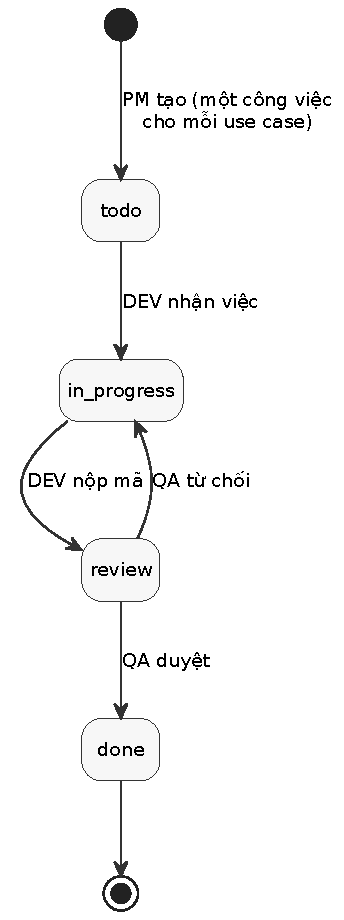
\includegraphics[height=0.32\textheight]{sodo/may-trang-thai-cong-viec.pdf}
\end{figure}

Đoạn mã~\ref{code:repo} là giao diện Repository của dự án. Giao diện nằm ở tầng miền và chỉ nhắc tới DTO của miền, không kiểu nào của Prisma lọt được vào đây.

\begin{codelisting}{Giao diện Repository của dự án ở tầng miền (rút gọn)}
\label{code:repo}
\begin{Verbatim}
// apps/api/src/domain/repositories/IProjectRepository.ts
export interface IProjectRepository {
  findById(id: string): Promise<ProjectDTO | null>;
  findAll(options?: {
    orderBy?: 'createdAt' | 'updatedAt';
    order?: 'asc' | 'desc';
  }): Promise<ProjectDTO[]>;
  create(data: CreateProjectData): Promise<ProjectDTO>;
  update(id: string, data: UpdateProjectData): Promise<ProjectDTO>;
}
\end{Verbatim}
\end{codelisting}

Lớp hiện thực \code{PrismaProjectRepository} nằm ở \code{src/infrastructure/persistence} và chỉ lấy những cột mà DTO cần. Chi tiết này nghe thì nhỏ nhưng đo được hẳn hoi. Kiểm thử tải cho thấy truy vấn danh sách dự án từng kéo về cả ngữ cảnh JSON của lượt chạy mới nhất rồi bỏ đi. Sửa xong, thời gian truy vấn giảm từ 46~ms xuống 9~ms.

\section{Tác tử}

Đoạn mã~\ref{code:base-agent} là phần lõi của \code{BaseAgent.execute()}. Mỗi lần gọi tạo một máy trạng thái riêng, hai bước \code{think} và \code{act} được uỷ cho chiến lược, còn việc phát sự kiện, chuyển trạng thái và dọn dẹp do lớp cơ sở lo.

\begin{codelisting}{Khung thuật toán của tác tử trong BaseAgent (rút gọn)}
\label{code:base-agent}
\begin{Verbatim}
// apps/api/src/modules/agents/base.agent.ts
async execute(input: AgentContext): Promise<AgentResult<TOutput>> {
  const context = this.prepareContext(input);     // theo RoleProfile
  const lifecycle = new AgentStateMachine(AgentState.IDLE);
  this.running.add(lifecycle);                     // mỗi lần chạy một máy
  try {
    await this.publish(new TaskAssignedEvent(/* ... */));
    this.transition(lifecycle, AgentState.THINKING, 'Starting');
    const thought = await this.thinkingStrategy.think(context);
    this.transition(lifecycle, AgentState.ACTING, 'Executing');
    const action = await this.actionStrategy.act(context, thought);
    this.transition(lifecycle, AgentState.COMPLETED, 'Done');
    // lưu ký ức, phát AgentCompletedTaskEvent, quay về IDLE ...
  } catch (error) {
    this.transition(lifecycle, AgentState.ERROR, (error as Error).message);
    // ...
  } finally {
    this.running.delete(lifecycle);
  }
}
\end{Verbatim}
\end{codelisting}

Mỗi vai trò có một tệp hồ sơ trong \code{modules/agents/profiles} và hai chiến lược trong \code{modules/agents/strategies}. NestJS tiêm danh sách tác tử vào qua token \code{AGENTS}, rồi \code{AgentOrchestrator} dựng bảng tra theo vai trò và báo lỗi ngay nếu có hai tác tử trùng vai trò. Muốn thêm vai trò thứ chín, người phát triển thêm một giá trị \code{AgentRole}, một hồ sơ, hai chiến lược và một dòng đăng ký provider. Bộ điều phối và bộ máy quy trình giữ nguyên.

Chiến lược hành động của BA, Architect, DEV và QC ghi sản phẩm qua \code{ProjectWorkspace}. \code{OoadArtifactService}, một Facade, dựng tài liệu và khung mã từ mẫu Handlebars. Nội dung LLM trả về được tách thành các khối \code{<CODE filepath="...">}, và từng đường dẫn được kiểm tra trước khi ghi.

Đoạn mã~\ref{code:decorator} là Decorator ghi chi phí. Lớp này hiện thực đúng giao diện \code{ILLMProvider} mà nó bọc, nên chiến lược tác tử không phân biệt được mình đang gọi nhà cung cấp gốc hay bản đã bọc. Nếu việc ghi nhật ký bị lỗi thì lời gọi chính vẫn chạy bình thường, chỉ có thêm một cảnh báo.

\begin{codelisting}{Decorator ghi chi phí lời gọi LLM (rút gọn)}
\label{code:decorator}
\begin{Verbatim}
// apps/api/src/modules/llm/usage-tracking.provider.ts
export class UsageTrackingLLMProvider implements ILLMProvider {
  constructor(
    private readonly inner: ILLMProvider,
    private readonly apiUsageService: ApiUsageService,
    private readonly usage: UsageContext,
  ) {}

  async chat(params: ChatParams): Promise<ChatResult> {
    const startTime = Date.now();
    const result = await this.inner.chat(params);
    await this.apiUsageService.logUsage({
      projectId: this.usage.projectId,
      agentRole: this.usage.agentRole,
      requestedModel: params.model,
      promptTokens: result.tokenUsage?.promptTokens ?? 0,
      completionTokens: result.tokenUsage?.completionTokens ?? 0,
      responseTimeMs: Date.now() - startTime,
      // ...
    }).catch(err => this.logger.warn(/* ... */));
    return result;
  }
}
\end{Verbatim}
\end{codelisting}

\section{Bộ máy quy trình}

\code{WorkflowEngine} giữ một bảng ánh xạ từ loại nút sang \code{NodeExecutionStrategy}. Giao diện chiến lược rất nhỏ, như Đoạn mã~\ref{code:node}: một thuộc tính cho biết loại nút và một phương thức thực thi.

\begin{codelisting}{Giao diện chiến lược thực thi nút}
\label{code:node}
\begin{Verbatim}
// apps/api/src/modules/workflow/strategies/node-execution-strategy.ts
export interface NodeExecutionStrategy {
  readonly type: NodeType;
  execute(node: WorkflowNode, run: WorkflowRunRecord,
          ctx: NodeExecutionContext): Promise<NodeResult>;
}
\end{Verbatim}
\end{codelisting}

Có bảy lớp hiện thực giao diện này: \code{AgentTaskStrategy}, \code{SubWorkflowStrategy}, \code{QualityGateStrategy}, \code{ConditionStrategy}, \code{ParallelStrategy}, \code{HumanApprovalStrategy} và \code{AgentCollaborationStrategy}. Khi có Redis, mỗi nút là một công việc BullMQ, tối đa 5 công việc chạy cùng lúc. Không có Redis thì nút chạy trực tiếp. Nút nào xong thì \code{handleJobCompletion} ghi bước kèm thời lượng, chụp memento và chọn cạnh kế tiếp. Nút vẫn lỗi sau các lần thử lại thì kết quả được đổi thành \code{failure}, để lượt chạy đi theo cạnh \code{onFail} hoặc dừng ở trạng thái \code{failed}.

Mẫu quy trình là lớp con của \code{WorkflowTemplate}, có danh sách tham số định kiểu (số, chuỗi, enum, boolean) được kiểm tra trước khi dựng định nghĩa quy trình. Ví dụ mẫu \textit{REST API backend} có tham số \code{database} kiểu enum. Giá trị này được đưa vào lời nhắc thiết kế của Architect như một ràng buộc của nút, để Repository được thiết kế đúng cho loại cơ sở dữ liệu đã chọn. Hình~\ref{fig:template-form} là phần cuối của hộp thoại tạo dự án. Các ô tham số được sinh ra từ danh sách tham số của mẫu, bên dưới có bản xem trước đồ thị quy trình kèm mã phiên bản.

\begin{figure}{Biểu mẫu tham số của mẫu quy trình}
\label{fig:template-form}
\centering
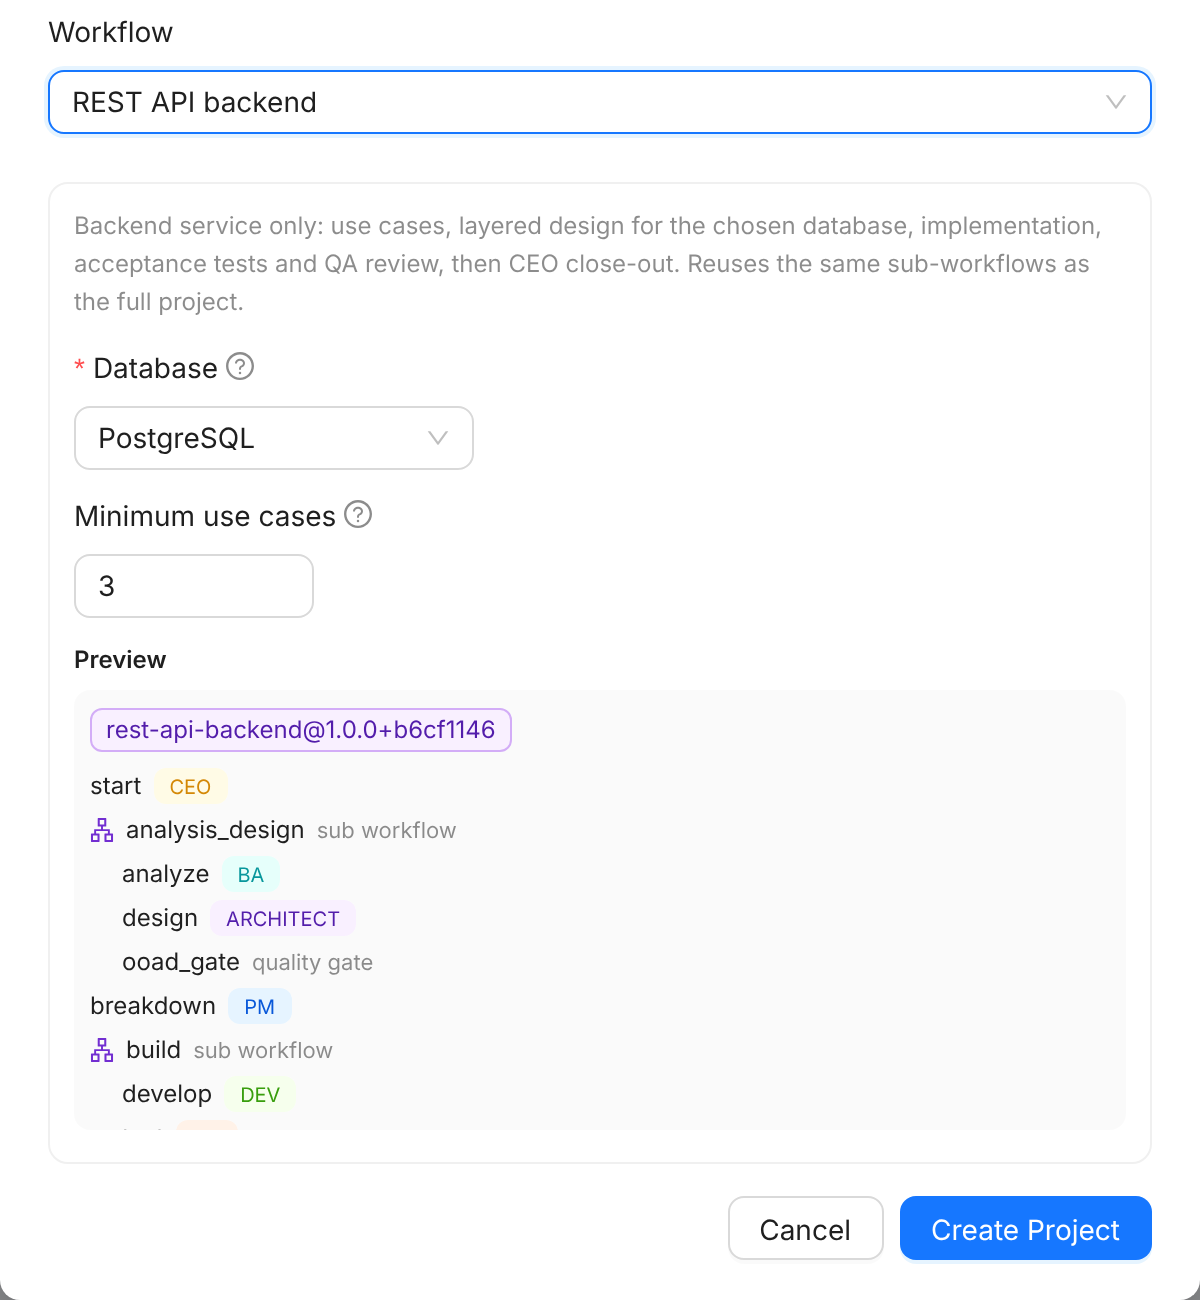
\includegraphics[width=0.5\textwidth]{anh/template-form.png}
\end{figure}

\section{Tính năng doanh nghiệp}

\begin{itemize}
\item \textbf{Phân quyền.} Controller gắn decorator \code{@RequirePermission} với tham số như \code{Permission.PROJECT_CREATE}, còn quyền của từng vai trò lấy từ gói \code{shared-types}. Giao diện giấu những nút mà người dùng không có quyền bấm, như nút \textit{New Project} với người xem, nhưng API vẫn tự kiểm tra quyền chứ không trông vào giao diện.
\item \textbf{Kiểm toán.} Route gắn \texttt{@Audited(\{ action: 'approval.approve', resourceType: 'Approval', idParam: 'id' \})}, và interceptor ghi kết quả \textit{ok} hoặc \textit{denied} kèm địa chỉ IP. Trang nhật ký có bộ lọc, phân trang và nút xuất CSV. Ô nào bắt đầu bằng \code{=}, \code{+}, \code{-}, \code{@} được thoát để chống chèn công thức khi mở bằng bảng tính. Trong Hình~\ref{fig:audit} có thể thấy ba loại tác nhân nằm chung một bảng: người dùng (đăng nhập, duyệt), tác tử (hoàn thành công việc) và hệ thống (kết thúc lượt chạy).
\item \textbf{Xuất báo cáo.} Hỗ trợ JSON, CSV và PDF. PDF dựng bằng pdfkit với phông chữ có dấu tiếng Việt. Báo cáo tuần được ghi vào thư mục \code{reports/} của dự án thay vì gửi email.
\item \textbf{Nhà cung cấp LLM.} Trang \textit{LLM Providers}, chỉ dành cho quản trị viên, cho phép thêm nhà cung cấp từ mẫu có sẵn, kiểm tra kết nối, lấy danh sách mô hình hoặc thêm mô hình theo mã (Hình~\ref{fig:providers}). Ở trang \textit{Agent Models}, quản trị viên chọn mô hình cho từng vai trò từ danh sách nhóm theo nhà cung cấp. Mọi thay đổi đều được ghi kiểm toán với khoá đã che.
\item \textbf{Điều khiển lượt chạy.} Đầu trang chi tiết dự án có nút tạm dừng, tiếp tục, huỷ, bắt đầu quy trình và chỉnh ngân sách. Một biểu ngữ báo khi ngân sách đã hết hoặc quy trình chưa bắt đầu. Phê duyệt được trả lời trong một hộp thoại có tóm tắt dễ đọc, và ai từ chối thì phải ghi lý do.
\end{itemize}

\begin{figure}{Trang nhật ký kiểm toán}
\label{fig:audit}
\centering
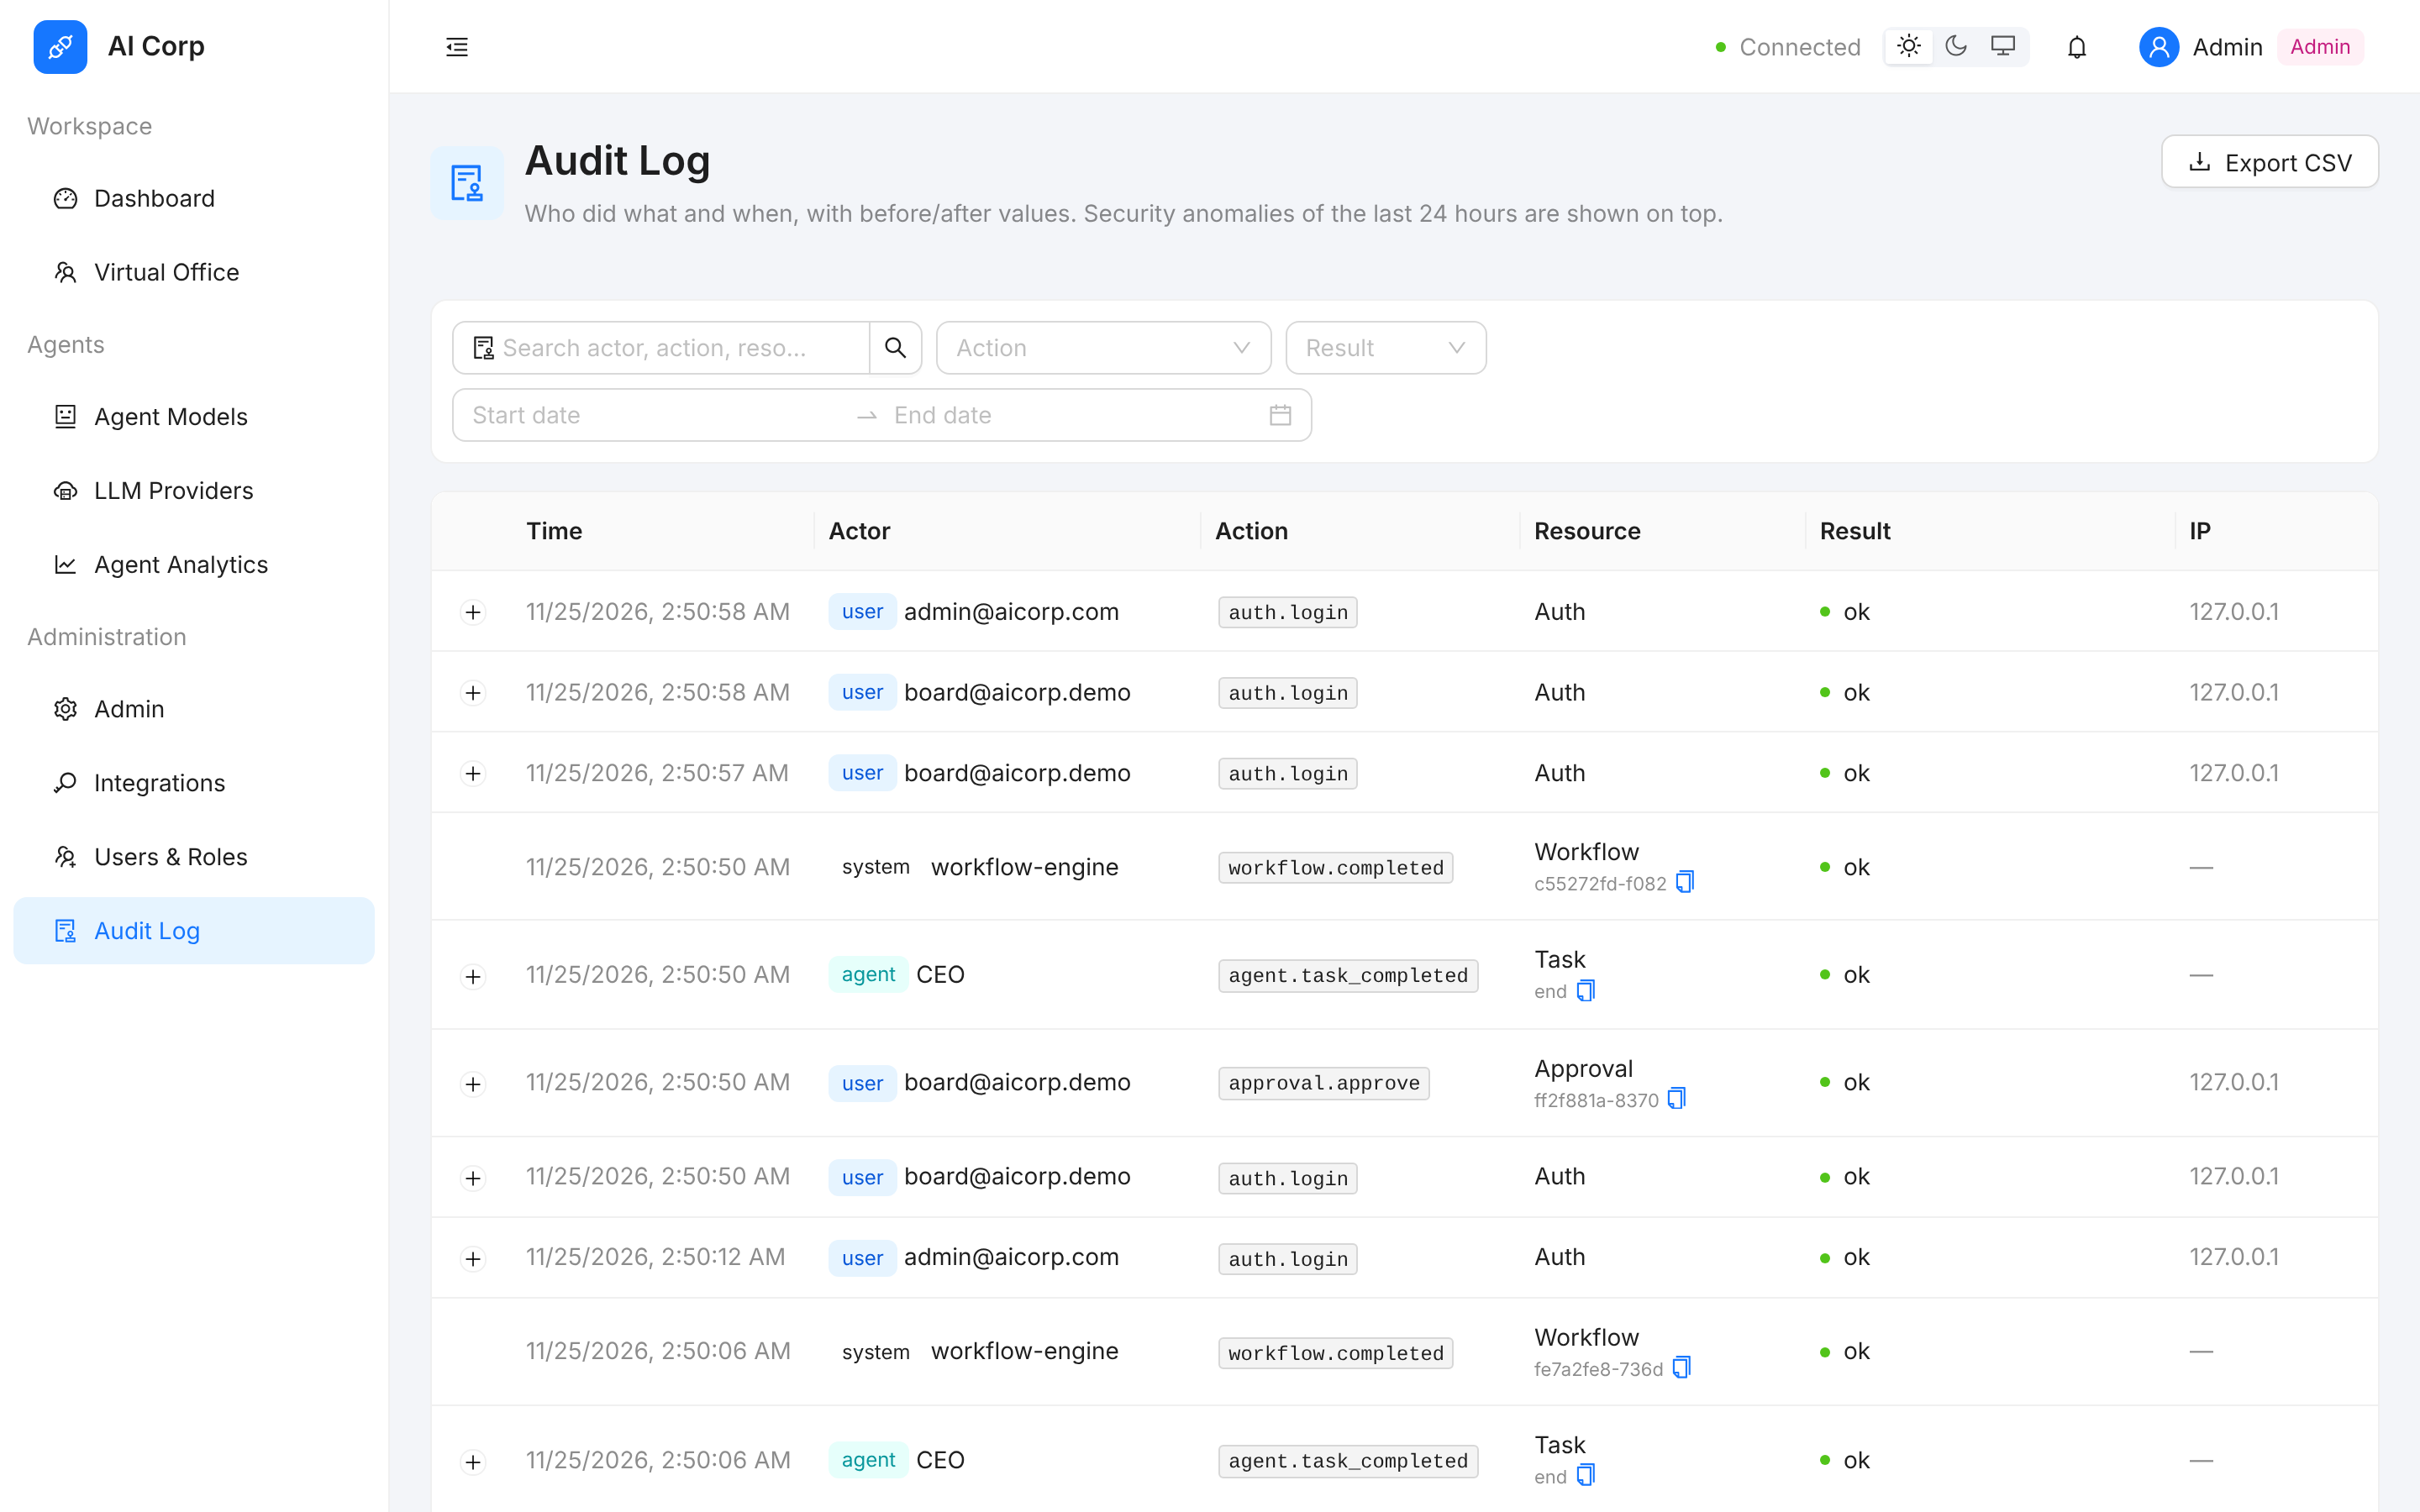
\includegraphics[width=\textwidth]{anh/audit-log.png}
\end{figure}

\begin{figure}{Trang quản lý nhà cung cấp LLM}
\label{fig:providers}
\centering
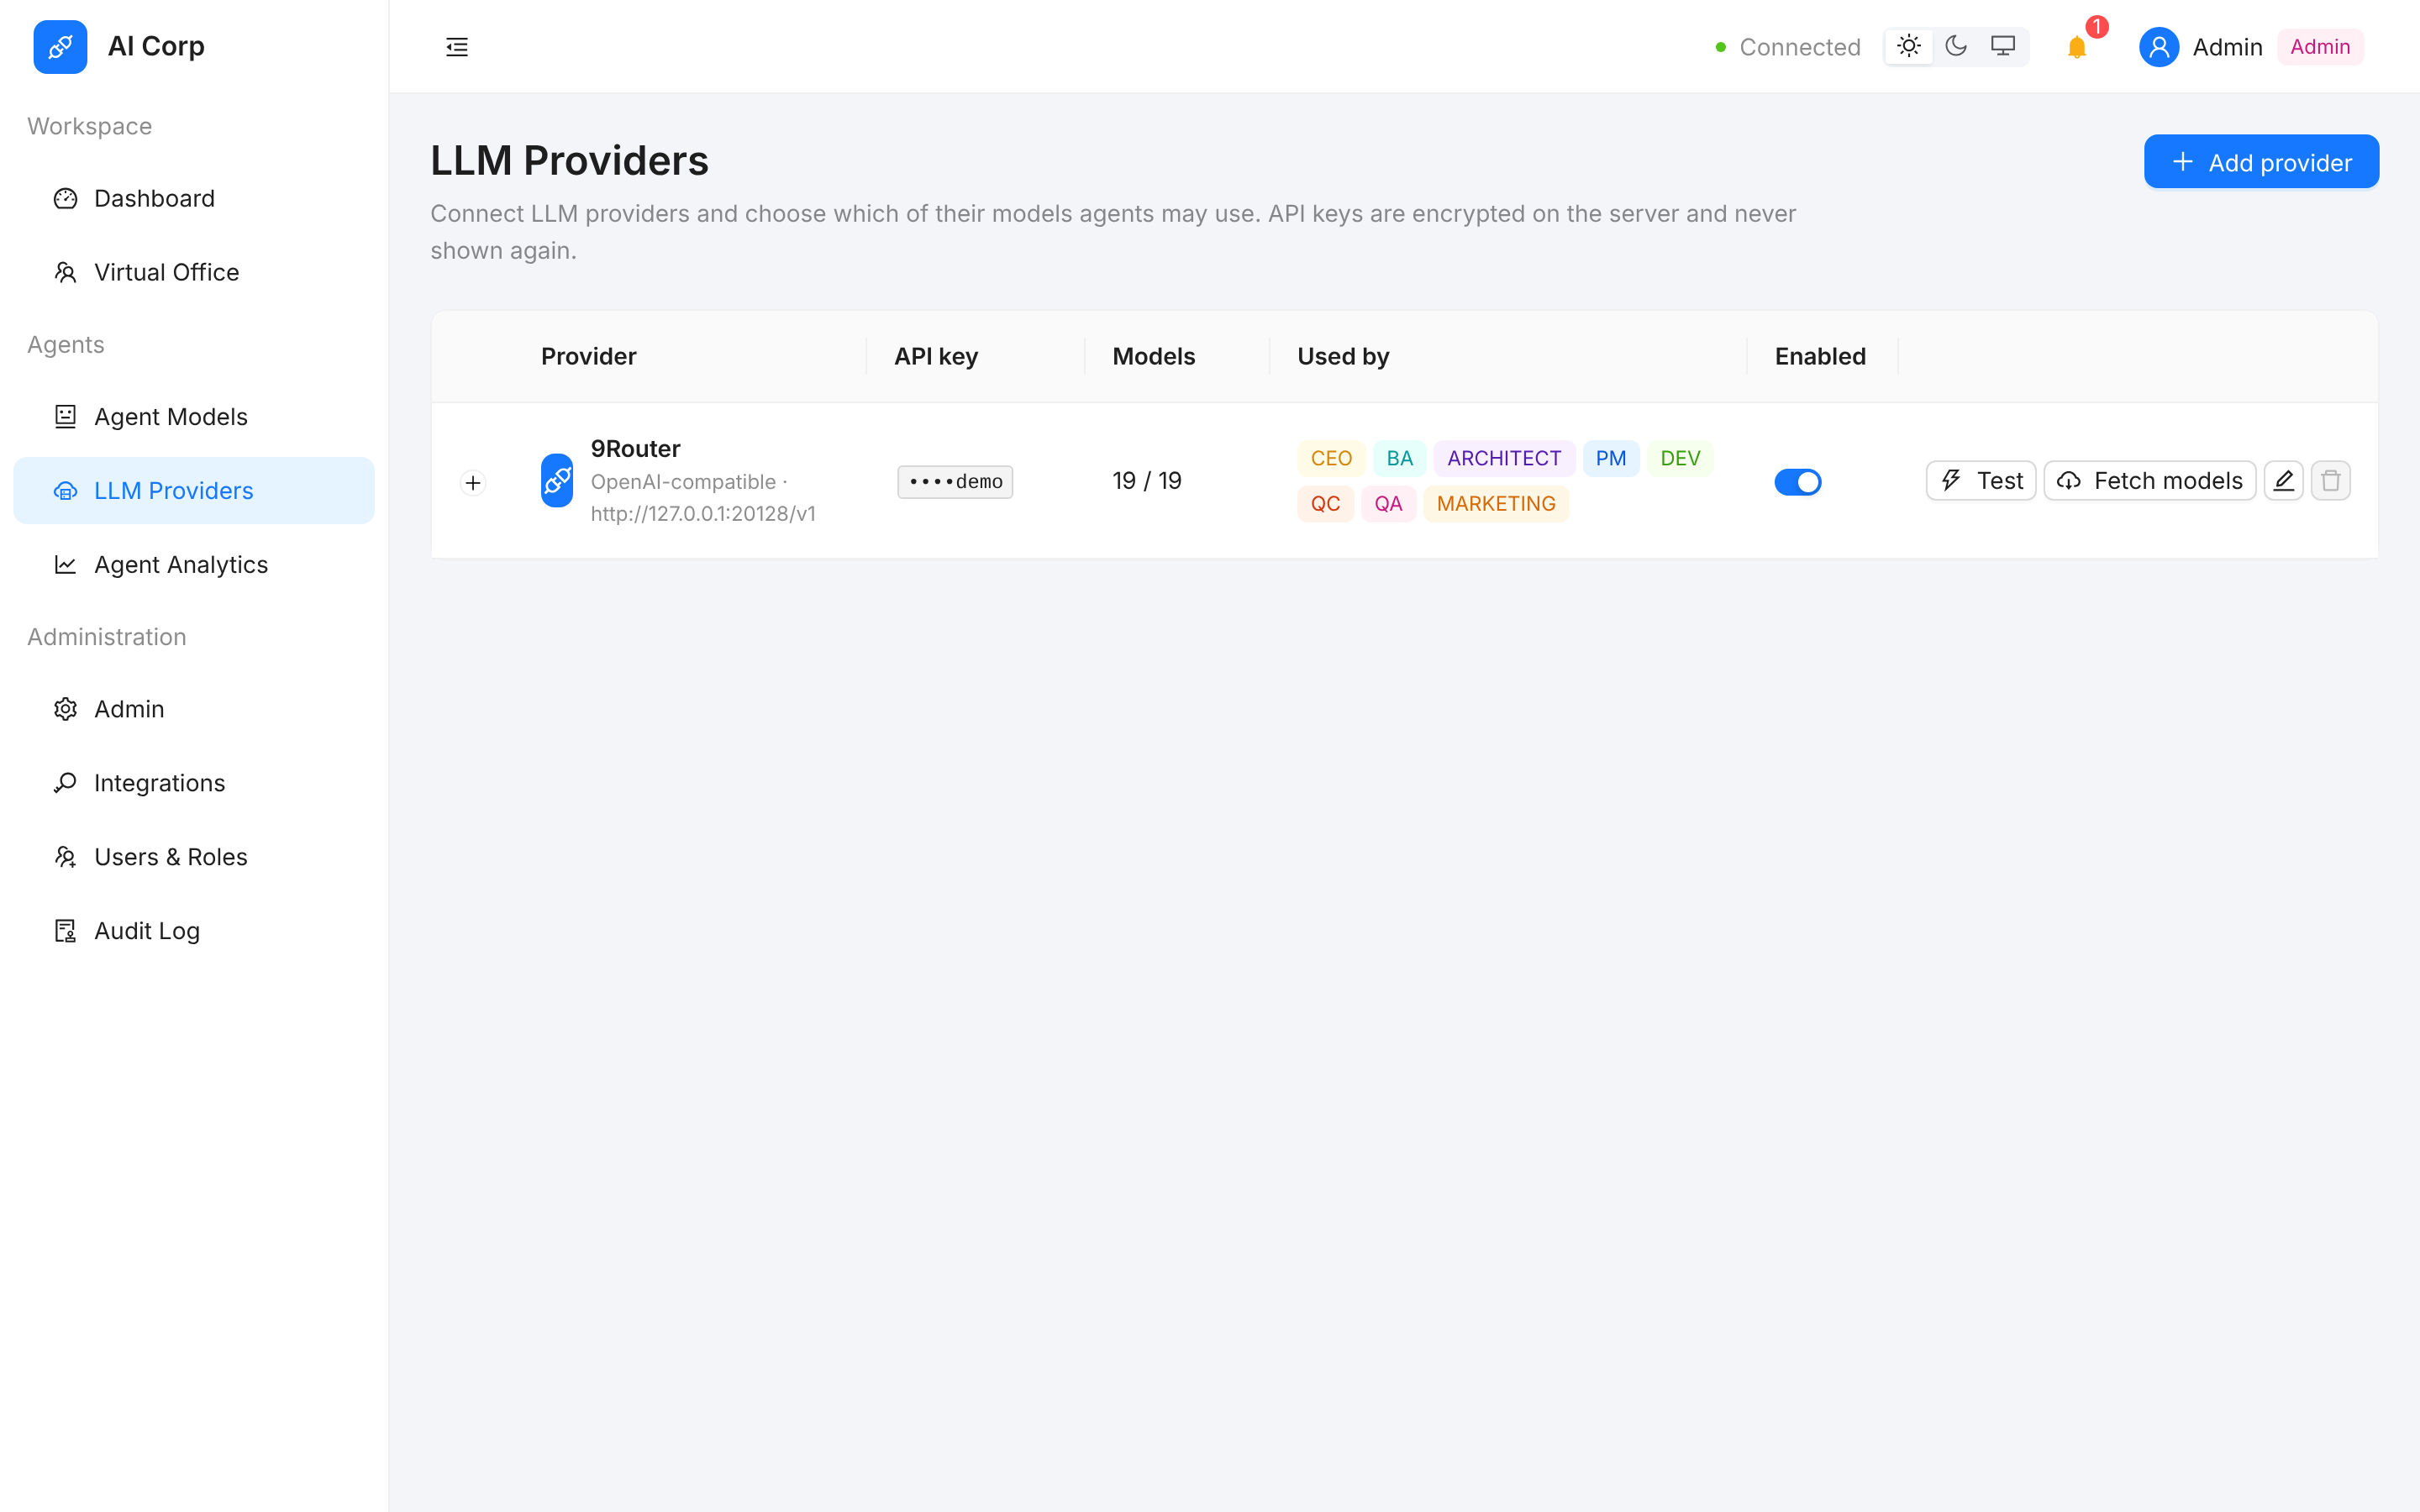
\includegraphics[width=\textwidth]{anh/providers.png}
\end{figure}

\section{Giao diện người dùng}
\label{sec:giao-dien}

Ứng dụng web viết bằng React và dùng nhãn tiếng Anh. Ở bản mới nhất, toàn bộ giao diện được chuyển sang Ant Design 6. Đợt nâng cấp này chỉ đụng tới phần hiển thị: logic, lời gọi API và tính năng giữ nguyên, và 44 kiểm thử web vẫn đạt như trước. Những thay đổi chính gồm:

\begin{itemize}
\item \textbf{Chủ đề giao diện.} \code{AppThemeProvider} gom màu sắc, cỡ chữ, bo góc vào các design token của Ant Design và xuất chúng thành biến CSS. Người dùng chọn chế độ sáng, tối hoặc theo hệ điều hành bằng ba nút ngay trên thanh đầu trang, và có thể bật chế độ gọn để bảng, biểu mẫu dày hơn. Lựa chọn được lưu trong trình duyệt qua một store Zustand. Mỗi vai trò tác tử được gán một tên màu có sẵn của Ant Design (CEO vàng, Architect tím, DEV xanh lá\ldots), và sắc độ cụ thể được chọn theo chế độ sáng hay tối.
\item \textbf{Khung trang mới.} Thanh bên chia nhóm \textit{Workspace}, \textit{Agents}, \textit{Administration}, thu gọn được về dạng biểu tượng, và chỉ hiện mục mà vai trò của người dùng được vào. Thanh đầu trang có chấm báo kết nối thời gian thực (\textit{Connected}), nút đổi chủ đề, chuông báo các phê duyệt đang chờ và menu tài khoản. Hai thành phần dùng chung \code{PageHeader} và \code{StatCard} giúp các trang có cùng một kiểu tiêu đề và thẻ số liệu.
\item \textbf{Dùng đúng thành phần cho từng việc.} Thông tin dự án và phê duyệt hiện bằng \code{Descriptions}, số liệu bằng \code{Statistic}, tiến trình và lịch sử bằng \code{Timeline} và \code{Steps}, cây tệp sản phẩm bằng \code{Tree}, khung xem tệp chia đôi bằng \code{Splitter}. Lúc đang tải thì hiện \code{Skeleton}, trang không có quyền hoặc không tồn tại thì hiện \code{Result}. Thông báo và hộp thoại đi qua \code{App.useApp()} để nhận đúng chủ đề đang dùng.
\item \textbf{Phòng họp và biểu đồ.} Khung trò chuyện của Phòng họp dựng lại bằng Ant Design X, thư viện thành phần dành cho giao diện AI, nên mỗi bước suy nghĩ của tác tử hiện thành một khối \textit{Thinking} mở ra xem được. Biểu đồ chi phí và phân tích chuyển từ Recharts sang Ant Design Charts (\code{@ant-design/plots}), dùng chung màu với chủ đề.
\item \textbf{Tải nhanh hơn.} Mỗi trang được tải lười (\code{React.lazy}) theo route, còn Vite tách React, Ant Design, Ant Design X và thư viện biểu đồ thành các gói riêng. Các gói thư viện ít đổi nên trình duyệt giữ được trong bộ đệm lâu hơn.
\end{itemize}

Các màn hình chính gồm \textit{Dashboard}, \textit{Virtual Office}, trang chi tiết dự án, \textit{Agent Models}, \textit{Agent Analytics}, \textit{LLM Providers}, \textit{Users \& Roles}, \textit{Audit Log} và \textit{Integrations}. \textit{Dashboard} liệt kê dự án, có tìm kiếm, lọc theo trạng thái, sắp xếp, và cho thấy tiến độ thật của lượt chạy cùng chi phí (Hình~\ref{fig:dashboard}). \textit{Virtual Office} hiện trạng thái tám tác tử theo thời gian thực bên cạnh Phòng họp. Trang chi tiết dự án có sáu tab: kết quả, sản phẩm, báo cáo, Kanban, mốc và lượt chạy. Tab \textit{Artifacts} gồm tóm tắt OOAD, kết quả cổng chất lượng, cây tệp, trình xem Markdown, mã nguồn, sơ đồ PlantUML do máy chủ PlantUML nội bộ render, và nút tải cả dự án về dạng zip.

\begin{figure}{Bảng điều khiển danh sách dự án ở chế độ sáng}
\label{fig:dashboard}
\centering
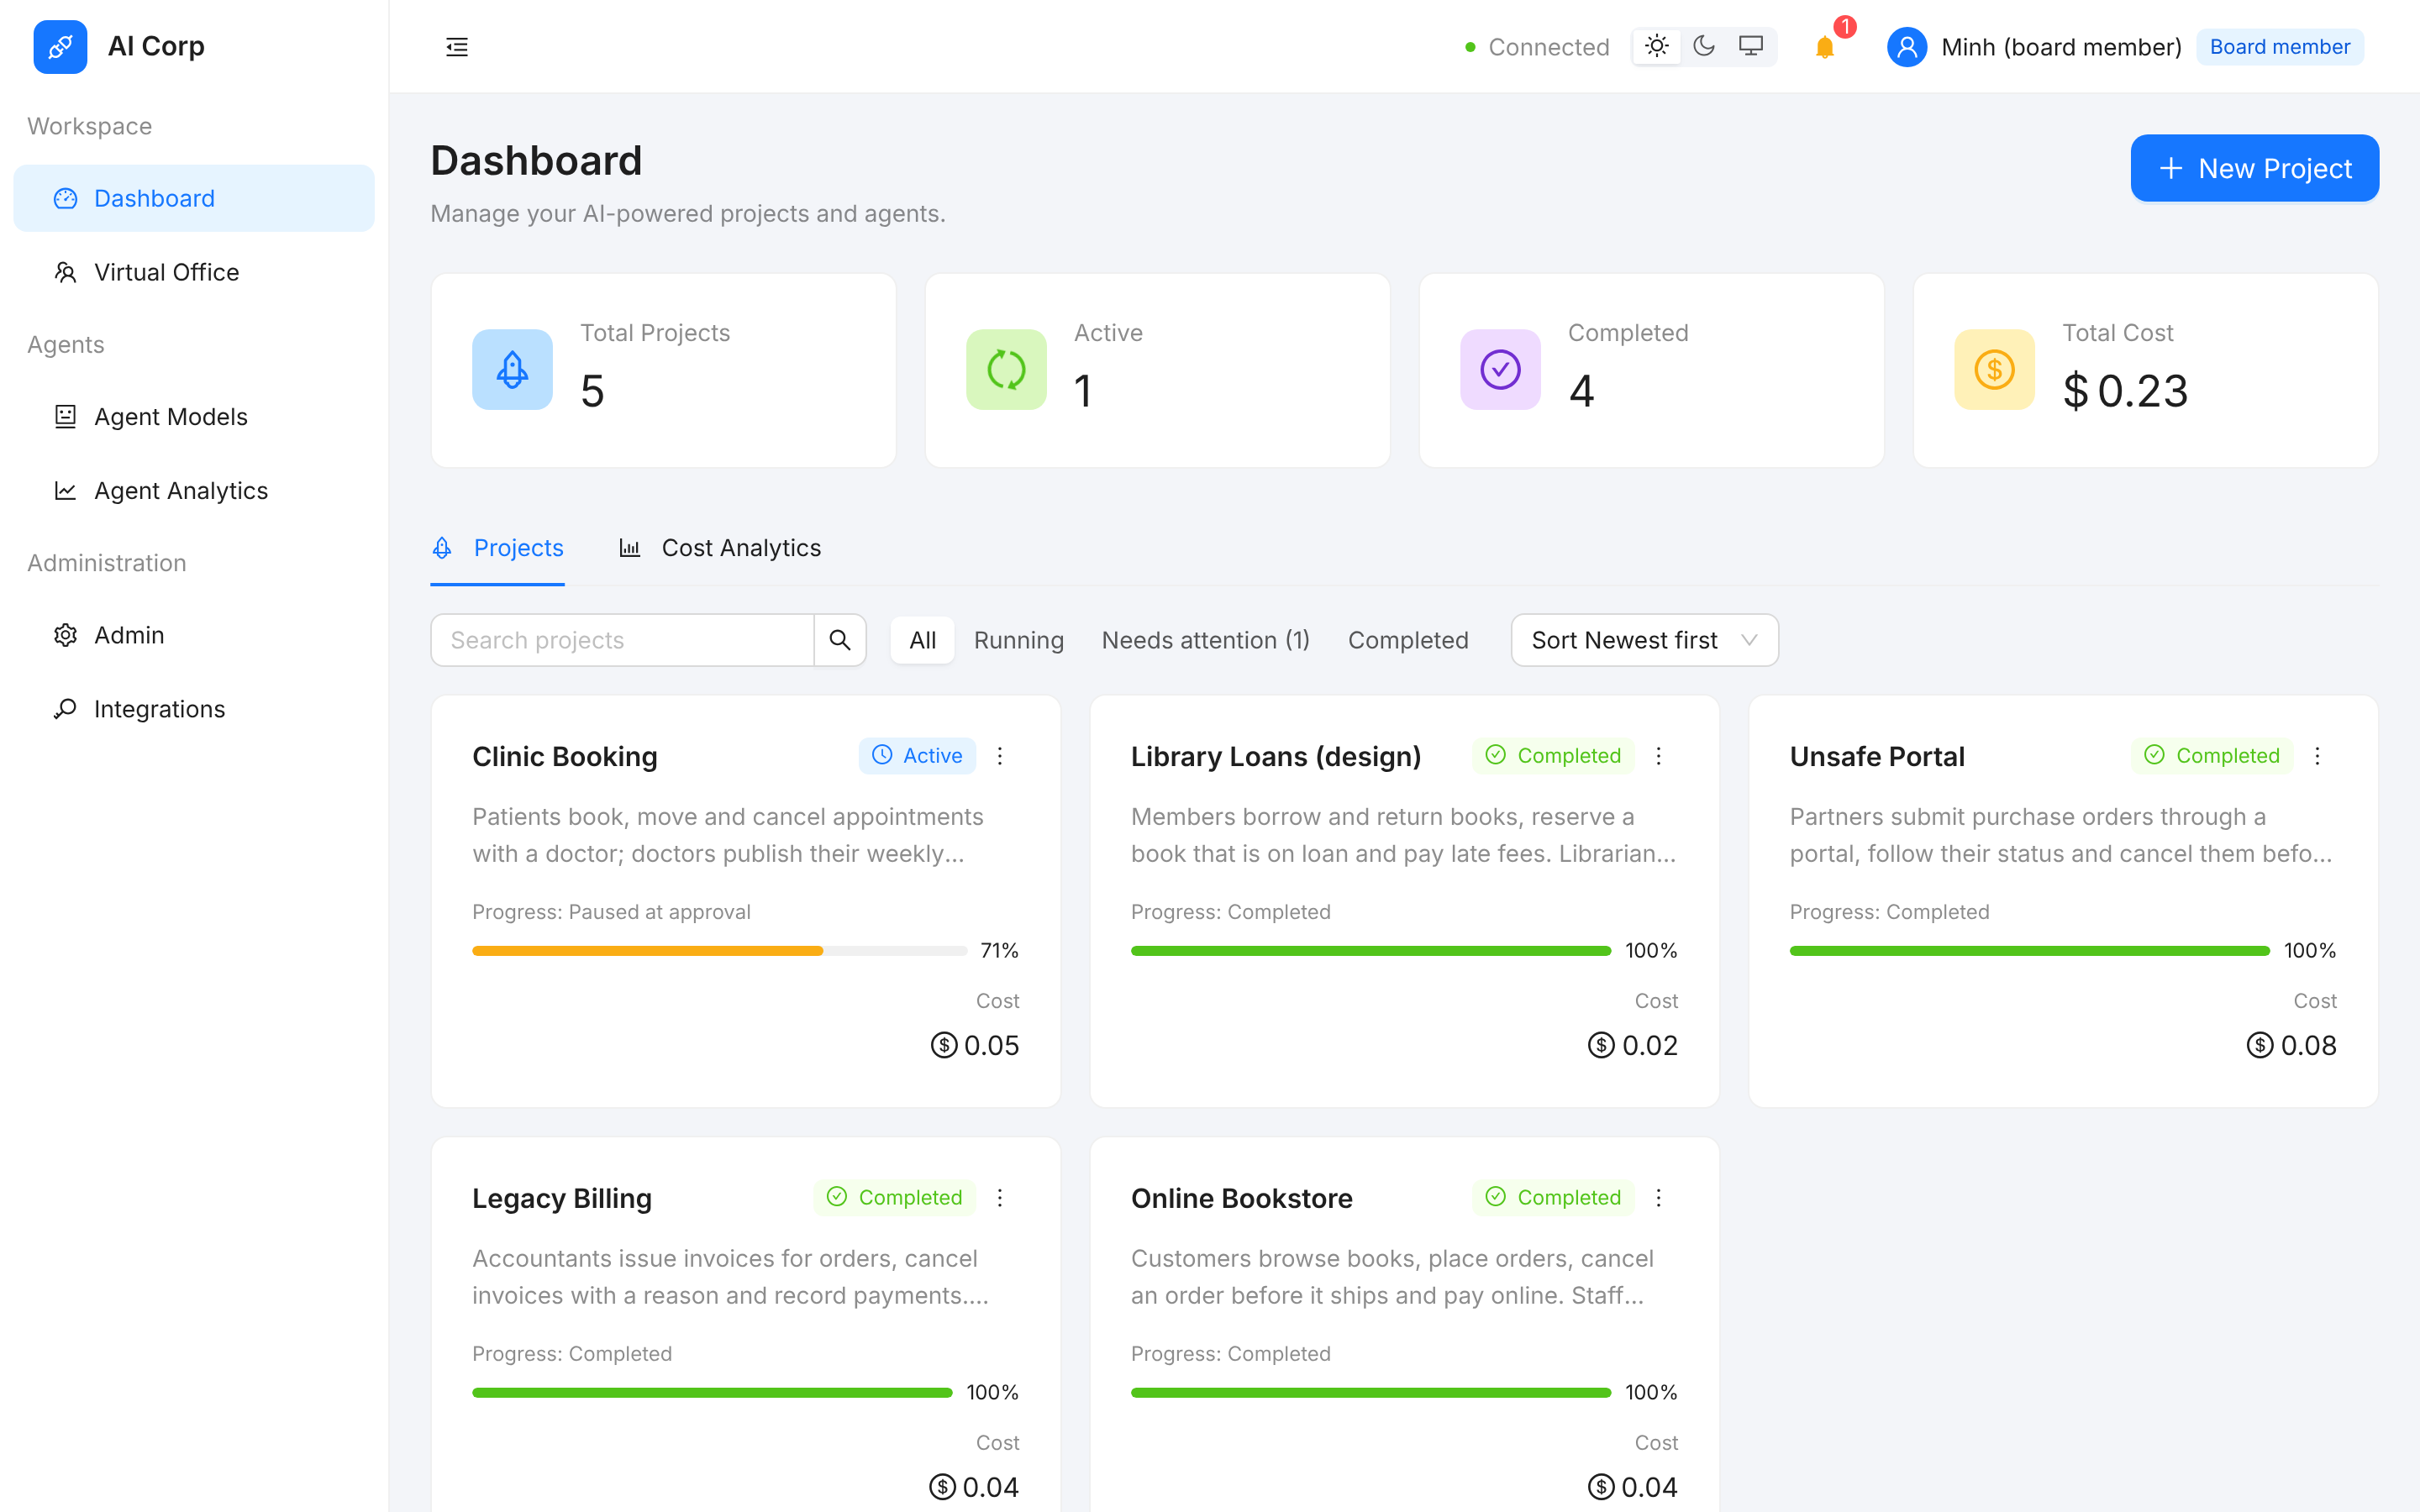
\includegraphics[width=\textwidth]{anh/dashboard.png}
\end{figure}

Hình~\ref{fig:timeline} là tab \textit{Workflow Runs} của dự án Unsafe Portal. Thanh tím là quy trình con, thanh xanh là từng bước của tác tử. Có thể thấy rõ vòng lặp: QA từ chối ở lần rà soát đầu, công việc quay lại DEV, rồi QC và QA chạy thêm một lượt. Bên dưới là danh sách ảnh chụp, mỗi ảnh có nút khôi phục, nút này chỉ bấm được khi lượt chạy đang tạm dừng hoặc đã lỗi.

\begin{figure}{Dòng thời gian và ảnh chụp của một lượt chạy quy trình}
\label{fig:timeline}
\centering
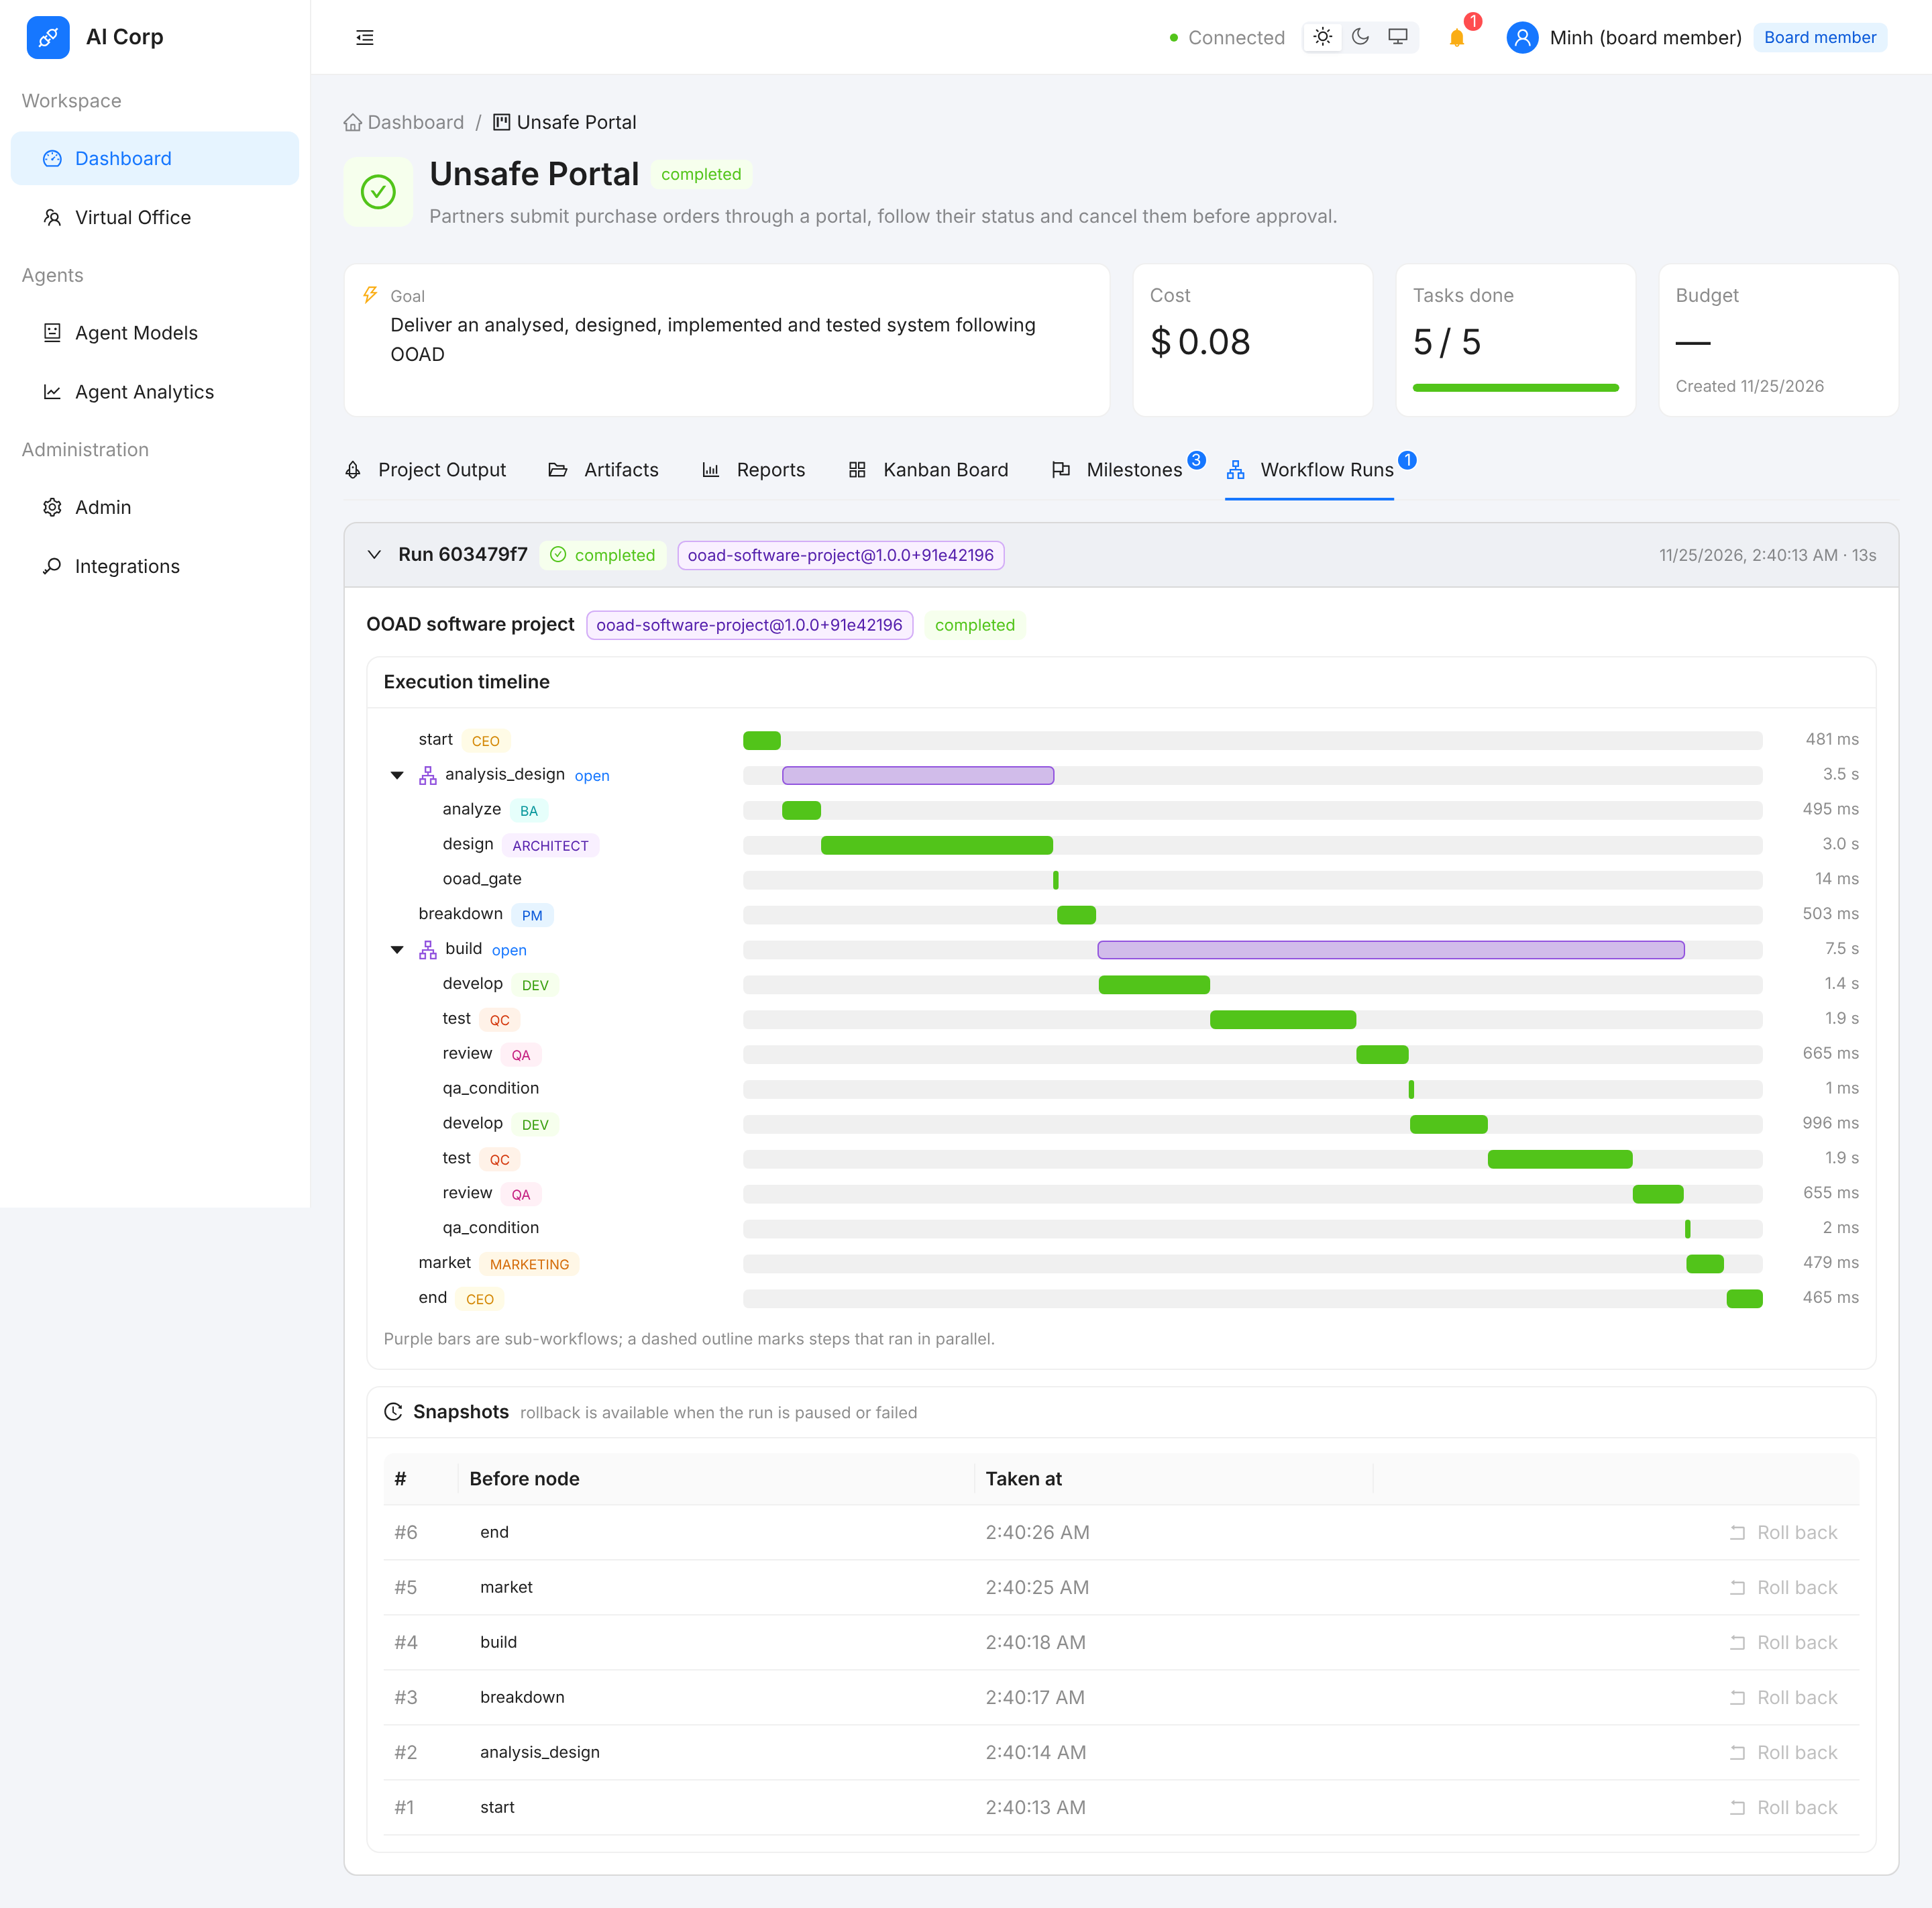
\includegraphics[width=0.85\textwidth]{anh/run-timeline.png}
\end{figure}

Khi chuẩn bị trình diễn, hai lỗi hiển thị được tìm thấy và sửa. Thẻ dự án lúc nào cũng hiện ``Starting\ldots{} 0\%'' vì dữ liệu danh sách dự án không kèm thông tin lượt chạy, còn tổng chi phí thì hiện số thực chưa làm tròn. Đợt rà soát giao diện sau đó tìm ra một lỗi nặng hơn. Trang dự án gửi yêu cầu vào phòng WebSocket với payload khác định dạng API chờ, nên sự kiện thời gian thực về công việc, quy trình và ngân sách không bao giờ tới được giao diện. Sau khi sửa, trang vào đúng phòng, tự vào lại khi mất kết nối và bỏ qua sự kiện trùng.

\section{Cấu hình triển khai}

\begin{itemize}
\item \code{apps/api/Dockerfile} có hai giai đoạn. Giai đoạn build cài phụ thuộc, sinh Prisma client, build API và script tạo dữ liệu ban đầu. Giai đoạn chạy dùng \code{tini}, chạy dưới người dùng \code{node}, có phông DejaVu cho xuất PDF và có HEALTHCHECK gọi \code{/api/health/live}. Tệp \code{docker-entrypoint.sh} chạy \code{prisma migrate deploy} rồi mới khởi động API.
\item \code{apps/web/Dockerfile} build ứng dụng với \code{VITE_API_URL=/api}, \code{VITE_WS_URL=/}, \code{VITE_PLANTUML_SERVER=/plantuml}, để mọi lời gọi đều cùng nguồn gốc qua nginx.
\item \code{docker-compose.prod.yml} và \code{.env.production.example} khai báo sáu dịch vụ (một dịch vụ chỉ chạy trong hồ sơ demo) và ba volume, chỉ công bố cổng web. Các biến môi trường mới gồm \code{LLM_SECRET_KEY}, \code{SIGNUP_ROLE}, \code{ALLOW_REGISTRATION} và \code{JWT_EXPIRATION}. Đổi \code{LLM_SECRET_KEY} thì phải nhập lại khoá của các nhà cung cấp.
\item Để cài mới từ mã nguồn, trường \code{packageManager} cố định pnpm 8.15.9, vì pnpm 8.0 lỗi trên Node 20 trở lên. Cấu hình Turborepo viết theo cú pháp của phiên bản đã cài và build gói \code{shared-types} trước. Tệp build-info của \code{shared-types} đặt trong \code{dist} để một bản clone mới luôn build ra mã.
\end{itemize}

Lúc chuẩn bị triển khai, bốn lỗi làm cấu hình cũ không chạy được đã lộ ra. Một, thư mục migration chỉ có lược đồ ban đầu, thiếu 8 bảng và nhiều cột, vì trong lúc phát triển nhóm dùng \code{prisma db push}. Hai, tệp khoá migration đặt sai chỗ. Ba, cấu hình nginx cắt mất tiền tố \code{/api}, khiến mọi lời gọi API trả 404 và WebSocket không được chuyển tiếp. Bốn, Dockerfile của API gọi điểm kiểm tra tình trạng sai đường dẫn và chạy một tệp không tồn tại. Cả bốn lỗi đều đã được sửa và kiểm chứng trong lần chạy đầu cuối triển khai ở chương sau.

\chapter{Kiểm thử và đánh giá}
\label{chap:kiem-thu}

Chương này nói về cách kiểm chứng nền tảng và những gì đo được. Con số nào cũng lấy từ một lần chạy có lưu vết trong kho mã, còn câu lệnh để chạy lại nằm ở Phụ lục~\ref{app:tai-tao}.

\section{Chiến lược kiểm thử}

Kiểm thử được sắp theo hình kim tự tháp~\cite{cohn2009}, gồm bốn tầng:

\begin{enumerate}
\item \textbf{Kiểm thử đơn vị} cho tầng miền, nơi hàm thuần không cần giả lập gì, và cho dịch vụ ứng dụng, nơi Repository, LLM và sandbox được thay bằng bản trong bộ nhớ.
\item \textbf{Kiểm thử tích hợp HTTP.} Dựng một ứng dụng Nest thật với guard, interceptor, controller thật, dữ liệu để trong bộ nhớ, rồi gọi vào qua HTTP.
\item \textbf{Kiểm thử đầu cuối} trên hạ tầng thật, gồm API đã build, PostgreSQL, Redis, nginx, một LLM kịch bản tương thích OpenAI và trình duyệt Playwright cho giao diện. Mỗi lần chạy có một tệp điều khiển, in ra một dòng cho mỗi kiểm tra và trả mã lỗi khác 0 nếu có kiểm tra hỏng.
\item \textbf{Kiểm thử tải} với ngân sách thời gian phản hồi cho từng endpoint.
\end{enumerate}

LLM kịch bản được dùng có chủ đích. Máy chủ này trả lời tuỳ theo nội dung lời nhắc, chẳng hạn dự án có tên bắt đầu bằng ``Legacy'' sẽ nhận bản mã đầu tiên vi phạm phân lớp. Độ trễ của nó tăng theo độ dài lời nhắc, và tên mô hình nó dùng có trong bảng giá. Nhờ vậy thời lượng và chi phí khác nhau giữa các dự án, đủ để huấn luyện mô hình dự báo, mà chạy lại bao nhiêu lần cũng ra đúng một kết quả.

\section{Kiểm thử tự động và độ bao phủ}

Bảng~\ref{tab:ket-qua-test} là kết quả của các bộ kiểm thử tự động. Mười lăm kiểm thử bị bỏ qua đều thuộc phần sandbox container, vì máy đo không có Docker daemon.

\begin{table}{Kết quả kiểm thử tự động}
\label{tab:ket-qua-test}
\begin{tabularx}{\textwidth}{|P{3.4cm}|L|}
\hline
\textbf{Bộ kiểm thử} & \textbf{Kết quả} \\ \hline
API (Jest) & 50 bộ, \textbf{707 đạt}, 15 bỏ qua, 0 thất bại \\ \hline
Web (Vitest) & 11 tệp, 44 đạt, chạy lại sau khi nâng cấp Ant Design 6 \\ \hline
Biên dịch & \code{nest build} 0 lỗi, \code{tsc --noEmit} của web 0 lỗi, \code{vite build} thành công \\ \hline
\end{tabularx}
\end{table}

Ngưỡng độ bao phủ được khai trong cấu hình Jest, nên chưa đạt thì lệnh \code{npm run test:cov} tự báo lỗi. Bảng~\ref{tab:bao-phu} đặt số đo cạnh ngưỡng.

\begin{table}{Độ bao phủ mã và ngưỡng}
\label{tab:bao-phu}
\small
\begin{tabular}{|l|r|r|r|r|c|}
\hline
\textbf{Phạm vi} & \textbf{Dòng} & \textbf{Lệnh} & \textbf{Hàm} & \textbf{Nhánh} & \textbf{Ngưỡng (dòng/lệnh/hàm/nhánh)} \\ \hline
Tầng miền & \textbf{97,1\%} & \textbf{96,2\%} & \textbf{97,0\%} & \textbf{88,1\%} & 90 / 90 / 90 / 85 \\ \hline
Toàn API & 77,8\% & 77,7\% & 74,4\% & 63,5\% & sàn 70 / 70 / 64 / 55 \\ \hline
\end{tabular}
\end{table}

Ngưỡng 90\% chỉ áp cho tầng miền chứ không áp cho cả API. Tầng miền chứa quy tắc nghiệp vụ, còn controller và phần nối với NestJS phần lớn là mã khung, đòi 90\% ở đó thì thực ra là đi kiểm thử lại framework. Tuy vậy, toàn API vẫn có một ngưỡng sàn để độ bao phủ không tụt dần theo thời gian.

\section{Kiểm thử đầu cuối}

Bảng~\ref{tab:e2e} tóm tắt ba lần chạy đầu cuối chính. Lần nào cũng bắt đầu từ cơ sở dữ liệu trống. Ngoài ba lần này còn có các lần chạy riêng cho bộ máy quy trình (quy trình con, ghim phiên bản, ảnh chụp và khôi phục, nhánh song song) và cho hệ thống tác tử (lưu sản phẩm OOAD, QC chạy kiểm thử, cơ chế học, lập trình cặp).

\begin{table}{Ba lần chạy kiểm thử đầu cuối chính}
\label{tab:e2e}
\small
\begin{tabularx}{\textwidth}{|P{3.4cm}|L|r|}
\hline
\textbf{Lần chạy} & \textbf{Nội dung} & \textbf{Kết quả} \\ \hline
Triển khai và trình diễn & Cấu hình production qua nginx, dữ liệu trình diễn, phân quyền, phê duyệt, xuất PDF, phân tích, kiểm toán, nhà cung cấp LLM & \textbf{24/24} \\ \hline
Phân tích, dự báo, chất lượng mã & 8 dự án chạy hết quy trình OOAD, rồi 3 lượt chạy khi mô hình của Marketing ngừng hoạt động, dùng bộ nhận webhook thật & \textbf{21/21} \\ \hline
Bảo mật, kiểm toán, tích hợp & Vai trò và quyền, nhật ký kiểm toán, khoá API, giới hạn tần suất, webhook ký HMAC, xuất dữ liệu, báo cáo & \textbf{44/44} \\ \hline
\end{tabularx}
\end{table}

Lần chạy triển khai kiểm tra những thứ mà kiểm thử đơn vị không nhìn thấy được:

\begin{itemize}
\item \code{prisma migrate deploy} dựng đúng lược đồ trên cơ sở dữ liệu trống qua ba migration, trong đó có migration cho bảng nhà cung cấp LLM. Lược đồ thu được không lệch so với mô hình (\code{prisma migrate diff --exit-code} trả 0).
\item API ở chế độ production từ chối khởi động khi cấu hình sai (thiếu \code{JWT_SECRET} và \code{CORS_ORIGIN}, khoá LLM là \code{CHANGE_ME}). Tiến trình thoát với mã 1 và in ra đủ cả ba lỗi.
\item Qua nginx, điểm kiểm tra tình trạng báo cơ sở dữ liệu, Redis và cổng LLM đều \textit{healthy}. Dừng PostgreSQL thì \code{/api/health} trả 503 trong khi \code{/api/health/live} vẫn trả 200; bật lại PostgreSQL thì kết quả trở về 200.
\item Swagger tắt khi \code{ENABLE_SWAGGER=false}, còn CORS chỉ trả header cho nguồn gốc đã cấu hình.
\item Kết nối WebSocket qua nginx nhận token hợp lệ và ngắt kết nối khi gặp token giả.
\item Người xem không tạo được dự án, không phê duyệt được qua REST và cũng không phê duyệt được qua WebSocket. Lỗ hổng ở kênh WebSocket được tìm ra và vá ngay trong lần chạy này (mục~\ref{sec:loi}).
\item Một phê duyệt chỉ trả lời được một lần, lần thứ hai nhận 409. Tài khoản tự đăng ký nhận vai trò người xem. Cổng LLM trong cấu hình được nhập thành nhà cung cấp đầu tiên với 19 mô hình, và API không trả khoá của nhà cung cấp này.
\item Sau khi thành viên hội đồng quản trị phê duyệt, CEO đóng dự án, và nhật ký kiểm toán có đủ \code{auth.login}, \code{project.create}, \code{approval.requested}, \code{approval.approve}, \code{access.denied}, \code{quality.gate.evaluated}, \code{workflow.completed}.
\end{itemize}

\begin{figure}{Hộp thoại phê duyệt của dự án Clinic Booking}
\label{fig:phe-duyet}
\centering
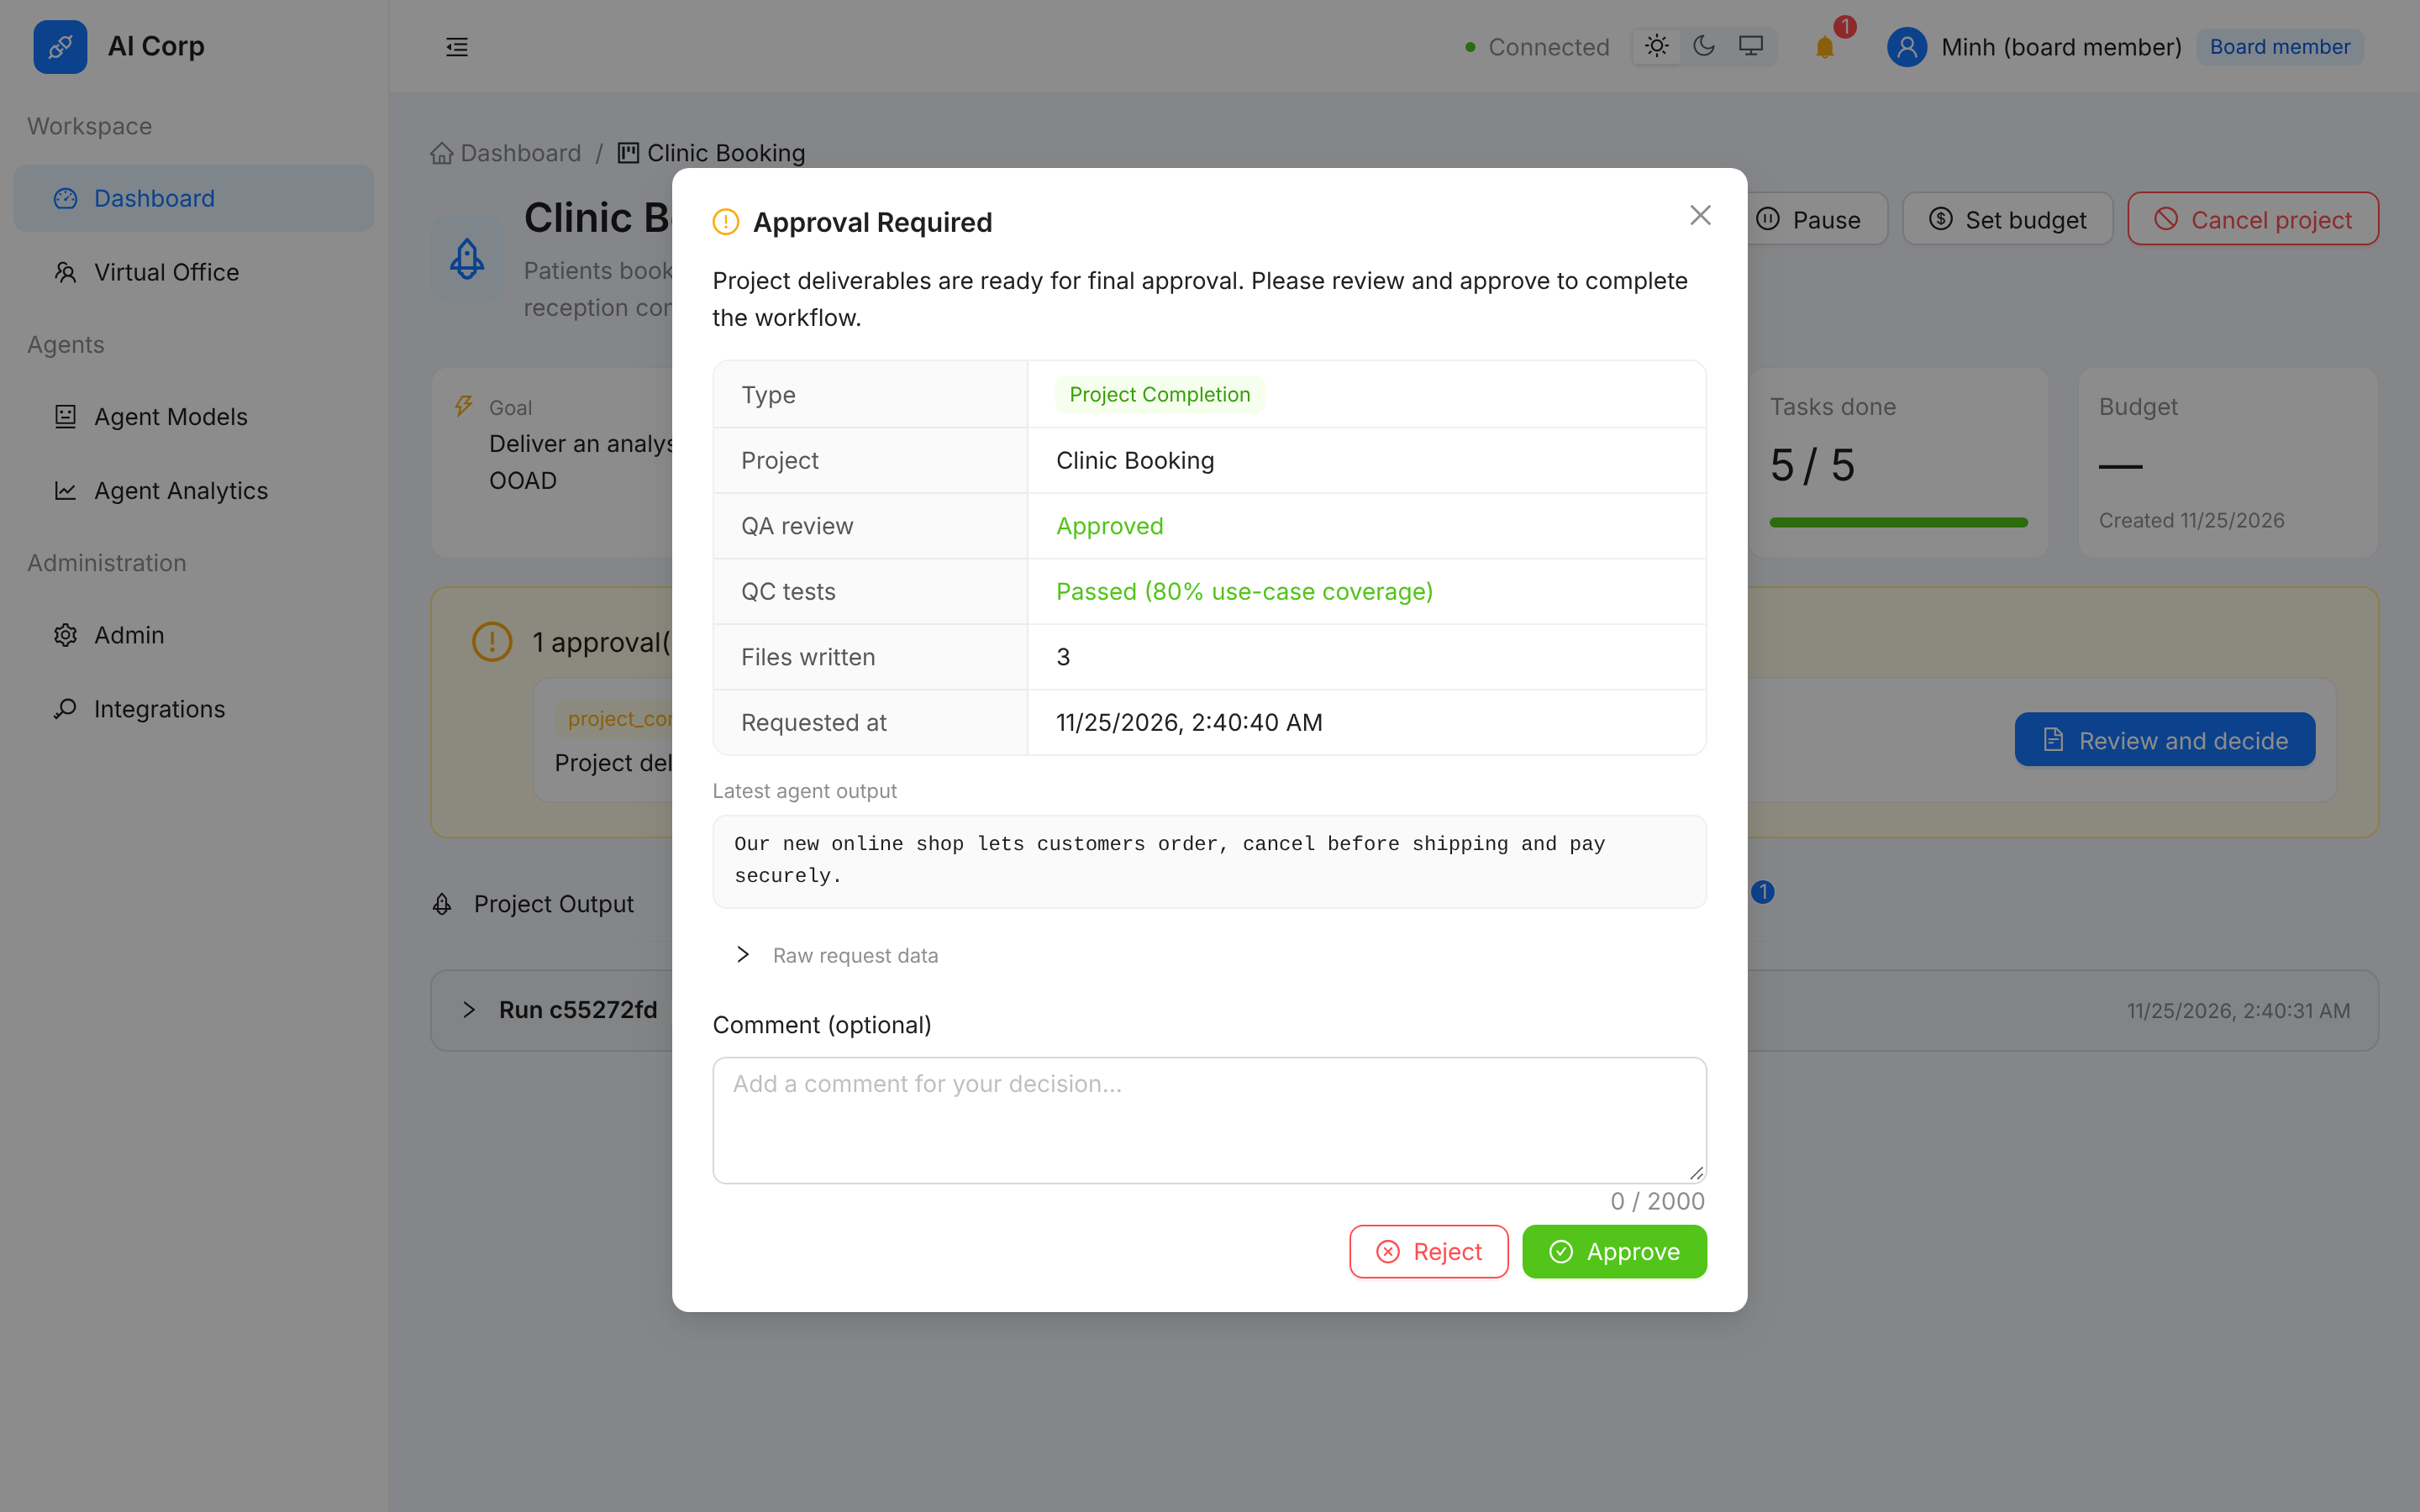
\includegraphics[width=\textwidth]{anh/approval.png}
\end{figure}

Hình~\ref{fig:phe-duyet} là hộp thoại mà thành viên hội đồng quản trị thấy khi bấm \textit{Review and decide} trên dự án Clinic Booking. Phần tóm tắt cho biết QA đã duyệt, QC đã chạy kiểm thử đạt với 80\% use case được bao phủ, kèm đầu ra mới nhất của tác tử. Dữ liệu thô của yêu cầu vẫn xem được nhưng được thu gọn lại.

\section{Thời gian xử lý một nút quy trình}

Theo yêu cầu phi chức năng, mỗi nút quy trình phải xong trong 2 giây, không tính độ trễ LLM, vì độ trễ đó tuỳ nhà cung cấp và nền tảng không điều khiển được. Bảng~\ref{tab:thoi-gian-nut} là thời lượng của 43 bước tác tử trong lần chạy triển khai. LLM kịch bản trả lời sau 20~ms cộng 1~ms cho mỗi 25 ký tự lời nhắc, nên các con số vẫn chứa một phần độ trễ giả lập.

\begin{table}{Thời lượng bước tác tử theo vai trò}
\label{tab:thoi-gian-nut}
\begin{tabular}{|l|r|r|r|r|}
\hline
\textbf{Vai trò} & \textbf{Số bước} & \textbf{p50 (ms)} & \textbf{p95 (ms)} & \textbf{Lớn nhất (ms)} \\ \hline
CEO & 10 & 75 & 100 & 100 \\ \hline
BA & 5 & 107 & 121 & 121 \\ \hline
Architect & 5 & 582 & 607 & 607 \\ \hline
PM & 4 & 105 & 110 & 110 \\ \hline
DEV & 5 & 614 & 632 & 632 \\ \hline
QC & 5 & 1\,642 & 1\,726 & 1\,726 \\ \hline
QA & 5 & 259 & 279 & 279 \\ \hline
Marketing & 4 & 75 & 81 & 81 \\ \hline
\textbf{Tất cả} & \textbf{43} & \textbf{110} & \textbf{1\,642} & p99: \textbf{1\,726} \\ \hline
\end{tabular}
\end{table}

Nút nào cũng xong dưới 2 giây. Kết quả gần như trùng với lần đo trước khi bộ máy thêm bước kiểm tra ngân sách trước mỗi nút (p50 108~ms, p95 1\,687~ms), tức là bước kiểm tra này hầu như không làm hệ thống chậm đi. QC chậm nhất vì tác tử này chạy thật bộ kiểm thử Jest của dự án sinh ra. Architect và DEV chậm hơn các vai trò còn lại vì phải ghi nhiều tệp và chạy phân tích tĩnh.

\section{Hiệu năng dưới tải}

Kiểm thử tải dùng một script không cần thư viện ngoài, đóng vai người dùng bảng điều khiển: xem danh sách và chi tiết dự án, công việc, báo cáo chi phí, phân tích tác tử, dự báo và chất lượng mã. Mỗi endpoint có ngân sách thời gian phản hồi p50/p95/p99, mặc định 100/500/1000~ms. Nhóm phân tích, dự báo và chất lượng mã được 300/1500/3000~ms, còn tạo dự án được 500/2000/3000~ms. Tỉ lệ lỗi tối đa là 1\%. Môi trường gồm một tiến trình API ở chế độ production, PostgreSQL và Redis, chạy trên máy 4 lõi dùng chung với bộ sinh tải và LLM kịch bản. Cơ sở dữ liệu bắt đầu với 5 dự án trình diễn và lớn dần khi kịch bản tạo thêm dự án. Kết quả nằm ở Bảng~\ref{tab:tai}.

\begin{table}{Kết quả kiểm thử tải}
\label{tab:tai}
\small
\begin{tabularx}{\textwidth}{|P{4.2cm}|r|r|L|}
\hline
\textbf{Kịch bản} & \textbf{Yêu cầu/s} & \textbf{Lỗi} & \textbf{Kết quả theo ngân sách} \\ \hline
1 người dùng & 184,7 & 0\% & Mọi endpoint trong ngân sách, p50 từ 3 đến 7~ms \\ \hline
20 người dùng, chỉ đọc & \textbf{604,8} & 0\% & Mọi endpoint trong ngân sách, p95 cao nhất 84~ms \\ \hline
20 người dùng, đồng thời tạo 111 dự án & 430,7 & 0\% & Mọi endpoint trong ngân sách, tạo dự án p50 107~ms, p99 177~ms \\ \hline
50 người dùng, tạo 48 dự án & 407,2 & 0\% & Bão hoà: p50 từ 77 đến 312~ms, năm endpoint vượt ngân sách p50 100~ms, mọi p99 dưới 0,7~s \\ \hline
\end{tabularx}
\end{table}

Với 50 người dùng, một tiến trình API đã bão hoà ở khoảng 407 yêu cầu mỗi giây. Theo định luật Little~\cite{little1961}, khi đó mỗi yêu cầu phải nằm trong hệ thống khoảng $50/407 \approx 123$~ms. Đây là giới hạn của một tiến trình đơn chứ không phải do truy vấn chậm. API không giữ trạng thái, vì lượt chạy được điều phối qua BullMQ và PostgreSQL, nên muốn phục vụ nhiều người hơn thì chạy thêm tiến trình.

Lần đo trước đó, trên cơ sở dữ liệu khoảng 120 dự án, cho 201,8 yêu cầu mỗi giây với 20 người dùng và bão hoà ở 178. Hai lần đo có lượng dữ liệu khác nhau nên không so thẳng được, và khoá luận không coi chênh lệch này là cải thiện. Cái so được là kết quả theo ngân sách. Ở cả hai lần, với 20 người dùng, mọi endpoint đều nằm trong hoặc sát ngân sách và không có lỗi. Lần đo trước đã chỉ ra ba lỗi hiệu năng (mục~\ref{sec:loi}). Sửa xong, p50 của endpoint chất lượng mã giảm từ 3,1~s xuống 196~ms trong cùng kịch bản.

\section{Độ chính xác của dự báo}

Sau khi 8 dự án chạy xong, vai trò nào cũng đủ mẫu để dùng mô hình hồi quy. Bảng~\ref{tab:mape} là sai số leave-one-out của dự báo thời gian tác tử.

\begin{table}{Sai số leave-one-out của dự báo thời gian theo vai trò}
\label{tab:mape}
\begin{tabular}{|l|r|}
\hline
\textbf{Vai trò} & \textbf{MAPE (LOO)} \\ \hline
Architect & 3\% \\ \hline
CEO & 5\% \\ \hline
BA & 11\% \\ \hline
DEV & 30\% \\ \hline
\end{tabular}
\end{table}

Xét dự báo lúc bắt đầu của 7 dự án (bỏ dự án đầu vì chưa có lịch sử), sai số tuyệt đối trung bình là 21\% về thời gian và 20\% về chi phí. Phần lớn sai số đến từ một dự án bị QA từ chối và DEV phải làm lại, làm chi phí vượt dự báo 84\%. Các dự án còn lại chỉ lệch từ 0 đến 10\%. Chuyện này dễ hiểu, vì lúc dự án vừa bắt đầu thì không ai biết trước nó có bị từ chối và phải làm lại hay không. Do đó nền tảng lưu cả dự báo lúc bắt đầu lẫn dự báo lúc PM lập kế hoạch, và luôn đặt dự báo cạnh số thực tế (Hình~\ref{fig:du-bao}). Trong hình, dự án Online Bookstore được dự báo 9,4~s và \$0,0587 dựa trên 4 dự án đã xong, còn thực tế đến lúc đó là 9,0~s và \$0,0538.

\begin{figure}{Dự báo công sức, chi phí và điểm chất lượng mã trong tab báo cáo}
\label{fig:du-bao}
\centering
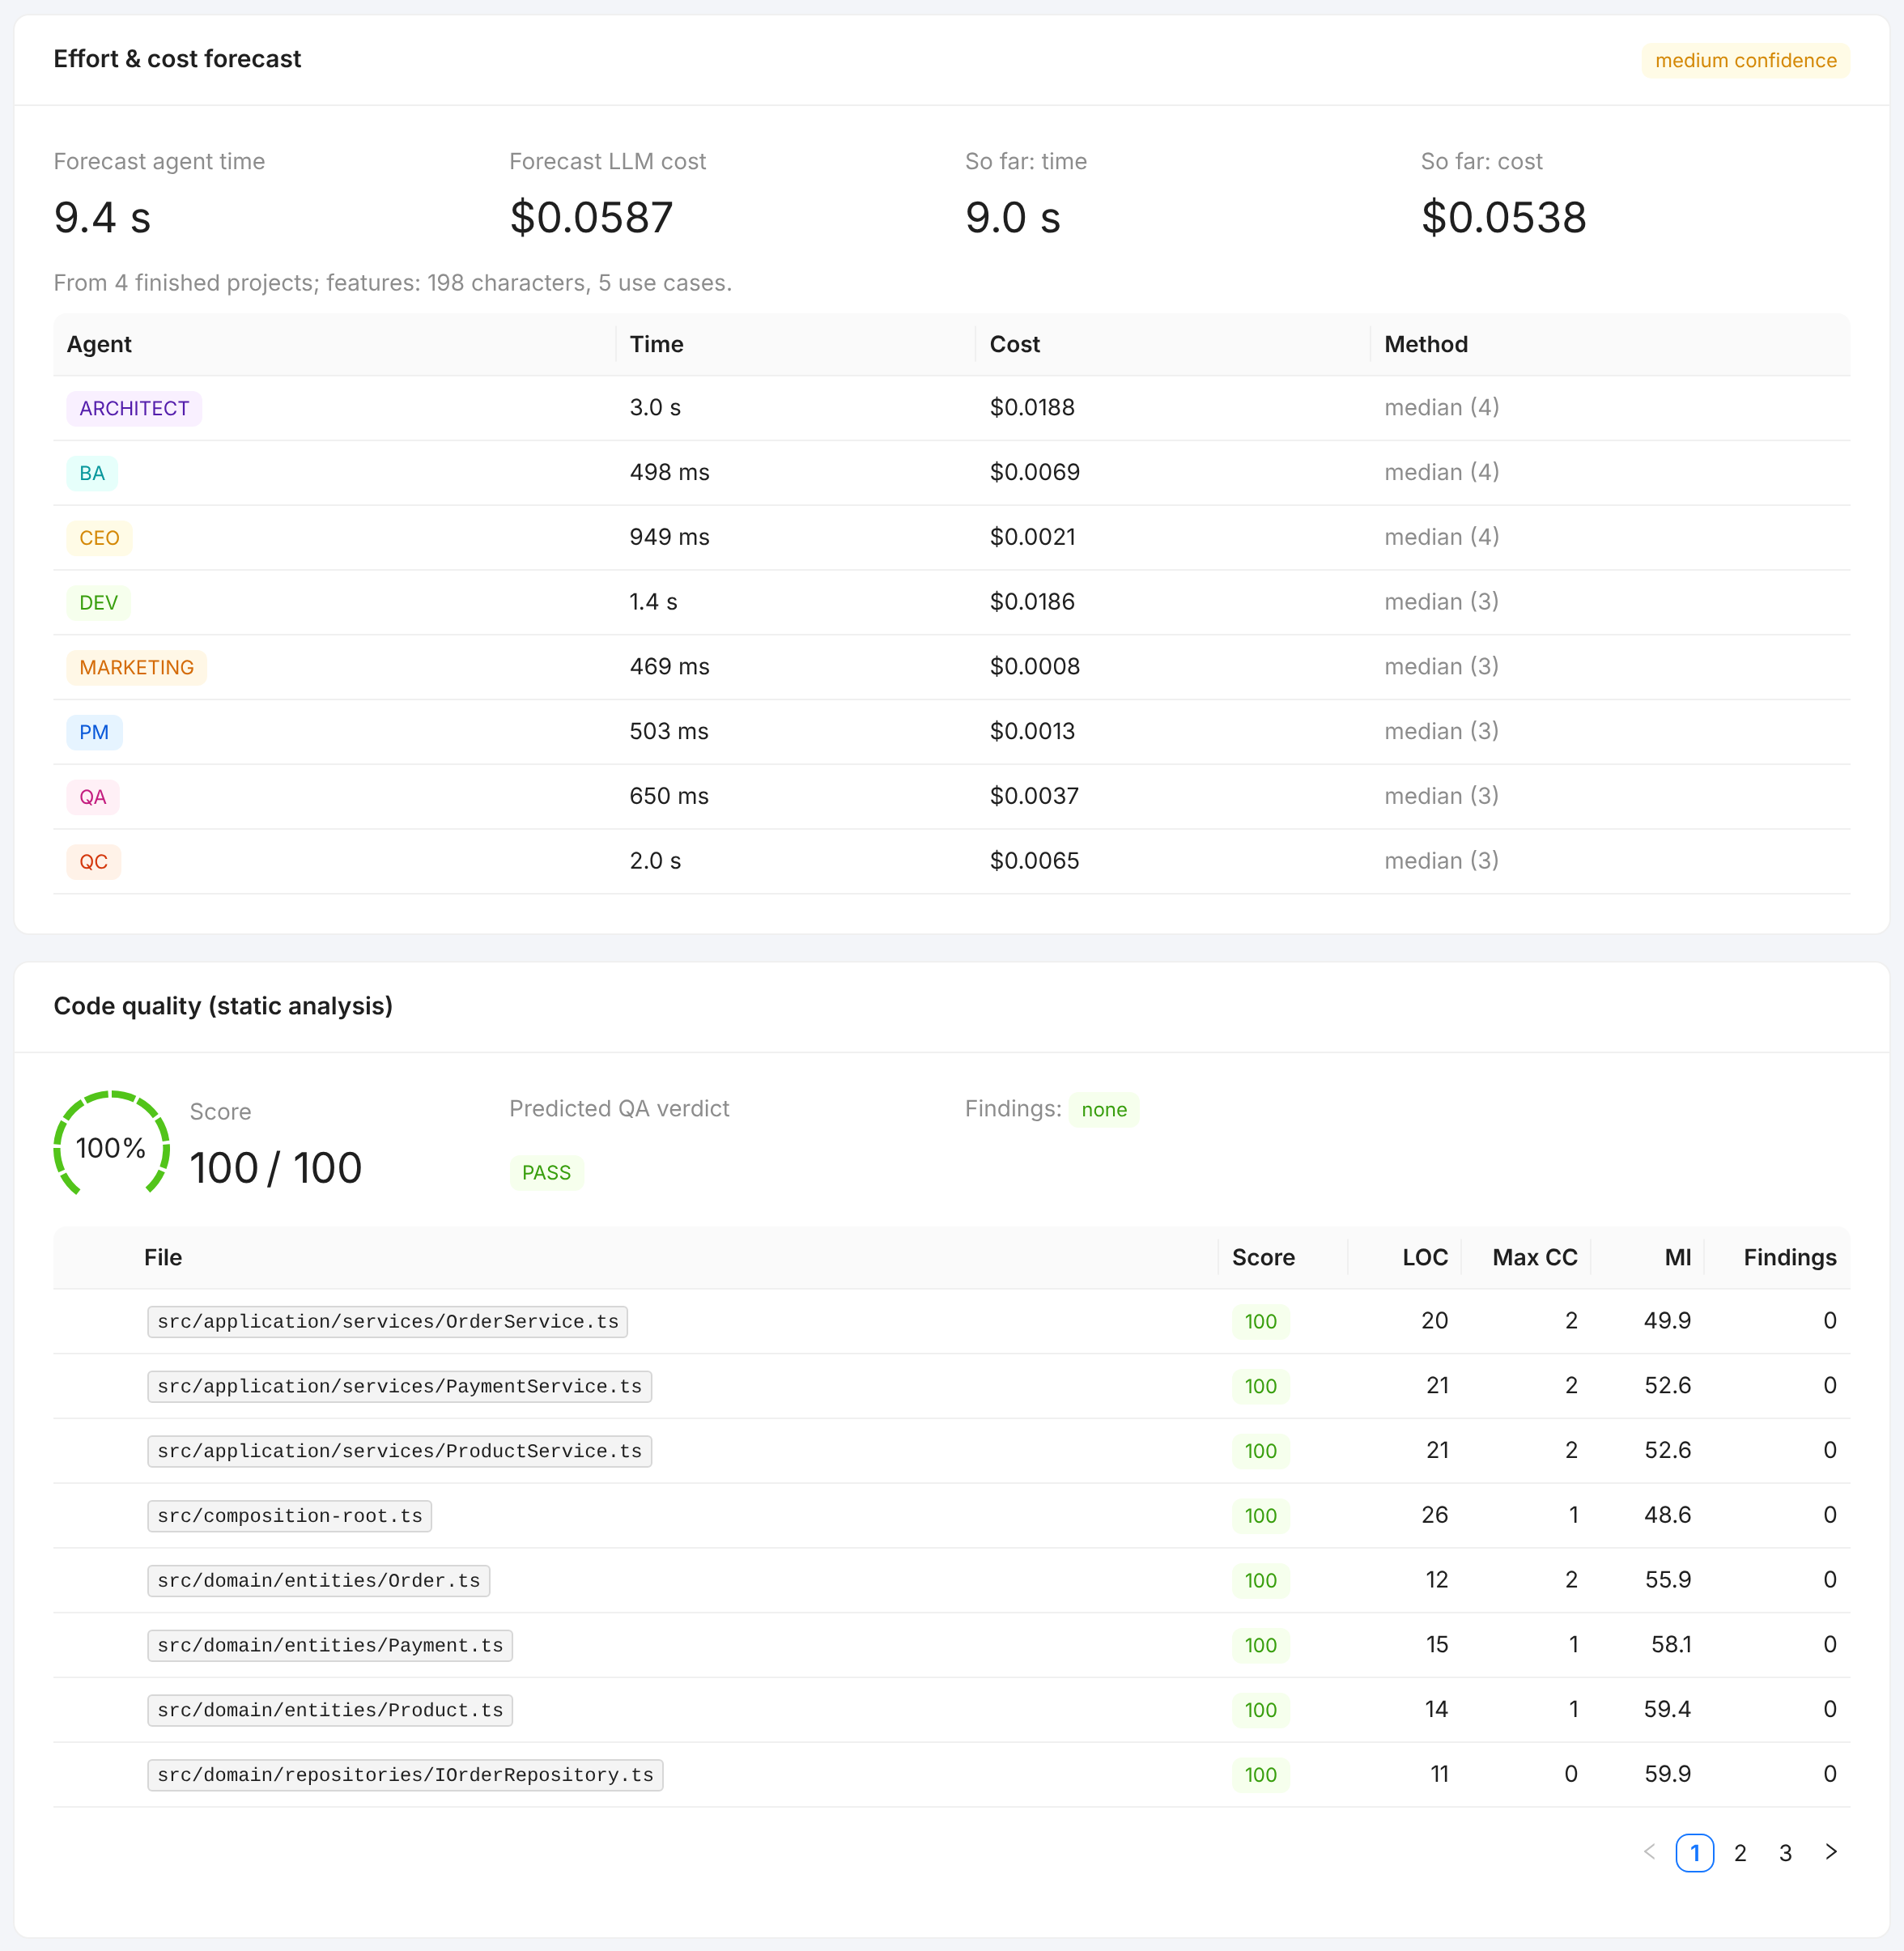
\includegraphics[width=0.85\textwidth]{anh/reports-forecast-quality.png}
\end{figure}

\section{Dự đoán chất lượng mã}

Bảng~\ref{tab:chat-luong-ma} kể lại chuyện gì đã xảy ra ở hai dự án được cài sẵn lỗi, và tổng kết trên tất cả các lần rà soát.

\begin{table}{Dự đoán phán quyết QA từ phân tích tĩnh}
\label{tab:chat-luong-ma}
\small
\begin{tabularx}{\textwidth}{|P{2.6cm}|L|}
\hline
\textbf{Trường hợp} & \textbf{Diễn biến} \\ \hline
Legacy Billing & Mã lần đầu của DEV nhập tầng hạ tầng từ tầng miền, có khoá viết cứng, gọi \code{eval} và dồn quy tắc vào một phương thức dài. Điểm 77 và có vi phạm phân lớp nên dự đoán là \textit{fail}. DEV sửa một vòng, điểm lên 100, bản sửa được giữ và QA duyệt. \\ \hline
Unsafe Portal & Vòng sửa không làm điểm tăng nên bản gốc được giữ. QA thấy \code{eval} trong báo cáo phân tích và trả FAIL. Quy trình quay về DEV, và lần thứ hai thì đạt. \\ \hline
Toàn bộ & Trong 9 lần QA rà soát, 8 lần dự đoán \textit{pass} và được duyệt, 1 lần dự đoán \textit{fail} và bị từ chối. \\ \hline
\end{tabularx}
\end{table}

Độ chính xác 100\% trên 9 lần rà soát phải đọc cẩn thận. Với LLM kịch bản, lỗi được cài sẵn đúng loại mà bộ phân tích bắt được. Con số này cho thấy chuỗi dự đoán, sửa và đối chiếu chạy đúng, nhưng chưa nói được gì về độ chính xác khi dùng LLM thật (mục~\ref{sec:hop-le}).

\section{Nghiên cứu tình huống}

Năm dự án trình diễn được tạo qua API công khai, giống hệt cách một người dùng thật sẽ làm. Mỗi dự án cho thấy một mặt của nền tảng (Bảng~\ref{tab:tinh-huong}). Với LLM kịch bản, cả năm dự án tạo và chạy xong trong khoảng 25 giây.

\begin{table}{Năm dự án trình diễn}
\label{tab:tinh-huong}
\small
\begin{tabularx}{\textwidth}{|P{2.4cm}|P{3.2cm}|L|}
\hline
\textbf{Dự án} & \textbf{Mẫu quy trình} & \textbf{Kết quả} \\ \hline
Online Bookstore & Dự án phần mềm OOAD & 5 use case, 3 thực thể, 3 mẫu thiết kế, đạt cổng OOAD 100\%, 35 tệp, 4 kiểm thử chấp nhận chạy đạt, độ bao phủ use case 80\% (UC-005 bị báo thiếu kiểm thử), có thông báo marketing, hoàn tất \\ \hline
Legacy Billing & Dự án phần mềm OOAD & Phân tích tĩnh phát hiện vi phạm, DEV tự sửa (điểm từ 77 lên 100) trước khi QA rà soát, hoàn tất \\ \hline
Unsafe Portal & Dự án phần mềm OOAD & QA từ chối, quy trình quay về DEV (2 bước DEV, 2 lần QA rà soát), hoàn tất \\ \hline
Library Loans & Chỉ phân tích và thiết kế & Use case, mô hình miền và sơ đồ vượt cổng OOAD, hoàn tất \\ \hline
Clinic Booking & Dự án phần mềm OOAD có phê duyệt & Dừng ở bước phê duyệt. Người xem không duyệt được. Thành viên hội đồng quản trị duyệt xong thì CEO đóng dự án \\ \hline
\end{tabularx}
\end{table}

Ở dự án Online Bookstore, độ bao phủ use case là 80\% chứ không phải 100\%. Chỗ này cho thấy chỉ số không bị làm đẹp. UC-005 không có kiểm thử nào chạy đạt nên không được tính, và ma trận truy vết ghi rõ là nó còn thiếu. Trên Hình~\ref{fig:artifacts}, dòng \textit{UC-005 missing} hiện ngay dưới thanh độ bao phủ.

\section{Lỗi phát hiện nhờ kiểm thử và rà soát}
\label{sec:loi}

Nhờ kiểm thử trên hạ tầng thật, khá nhiều lỗi đã được tìm ra và sửa. Ngoài kiểm thử tự động, lỗi còn lộ ra từ hai nguồn khác. Một là đợt rà soát mã giao diện và logic, trong đó từng màn hình được đọc và so với API mà nó gọi. Hai là lần cài lại từ mã nguồn trên một máy khác. Bảng~\ref{tab:loi} gom lỗi theo nhóm, còn danh sách đầy đủ kèm cách sửa nằm trong kế hoạch dự án và lịch sử thay đổi của kho mã.

\begin{table}{Lỗi phát hiện theo nhóm và theo nguồn}
\label{tab:loi}
\small
\begin{tabularx}{\textwidth}{|P{2.8cm}|L|r|r|r|r|}
\hline
\textbf{Nhóm} & \textbf{Ví dụ tiêu biểu} & \textbf{KT} & \textbf{RS} & \textbf{CĐ} & \textbf{Tổng} \\ \hline
Không khởi động, không chạy được & API không khởi động vì hai chiến lược có tham số hàm tạo mà DI không giải được; migration thiếu 8 bảng; nginx cắt tiền tố \code{/api}; pnpm 8.0 lỗi trên Node 20; bản clone mới không build ra \code{shared-types}; script dữ liệu trình diễn hỏng khi đăng ký mặc định thành người xem & 6 & 0 & 4 & 10 \\ \hline
Bảo mật & Duyệt qua WebSocket bỏ qua kiểm tra quyền và kiểm toán; ba giá trị dự phòng khác nhau cho khoá JWT; tự đăng ký nhận quyền thành viên hội đồng; một phê duyệt trả lời được hai lần; sửa công việc không kiểm tra chủ dự án & 3 & 3 & 0 & 6 \\ \hline
Thiết kế OOAD không được dùng & 4 trên 8 tác tử vẫn chạy luồng cũ nên chiến lược thành mã chết; cổng chất lượng không được đăng ký; sản phẩm tác tử mất sau mỗi lệnh sandbox; quy trình lập kế hoạch trước khi có yêu cầu & 6 & 0 & 0 & 6 \\ \hline
Tính đúng của quy trình và trạng thái & Một máy trạng thái cho mỗi vai trò; nút lỗi để lượt chạy \code{running} mãi; \textit{Pause} chỉ đổi trạng thái dự án; \textit{Resume} ở bước phê duyệt tạo phê duyệt trùng; dự án đã huỷ bị đánh dấu hoàn tất; lý do từ chối không tới được tác tử & 8 & 6 & 0 & 14 \\ \hline
Chi phí và sự kiện & Chi phí LLM của 4 vai trò không được ghi; nút vẫn chạy khi hết ngân sách; cộng chi phí kiểu đọc rồi ghi mất cập nhật khi đồng thời; thiếu sự kiện \code{approval.requested} và \code{workflow.failed} & 4 & 3 & 0 & 7 \\ \hline
Hiệu năng & Phân tích lại mọi tệp ở mỗi yêu cầu (3,1~s); danh sách dự án tải JSON không dùng; bốn truy vấn chạy tuần tự & 3 & 0 & 0 & 3 \\ \hline
Tài liệu và giao diện & 12 trên 39 sơ đồ UML không render được; thẻ dự án luôn hiện 0\%; trang dự án tham gia phòng WebSocket sai payload nên không nhận sự kiện thời gian thực & 3 & 1 & 0 & 4 \\ \hline
\textbf{Tổng} & & \textbf{33} & \textbf{13} & \textbf{4} & \textbf{50} \\ \hline
\end{tabularx}

\vspace{0.2cm}
{\footnotesize KT: kiểm thử, RS: rà soát mã, CĐ: cài đặt mới từ mã nguồn.}
\end{table}

Cả mười ba lỗi do rà soát tìm ra đều nằm trên những luồng mà kiểm thử tự động chưa đi tới. Các kiểm thử đầu cuối chạy quy trình từ đầu tới cuối, nhưng không tạm dừng rồi tiếp tục, không trả lời một phê duyệt hai lần và không cộng chi phí hai lần cùng lúc. Sau khi sửa, mỗi lỗi có một kiểm thử đơn vị riêng (\code{run-control.spec.ts}, \code{approval-and-signup.spec.ts}), và ba hành vi được thêm vào lần chạy đầu cuối triển khai: phê duyệt chỉ trả lời được một lần, tài khoản tự đăng ký chỉ nhận quyền xem, và khoá nhà cung cấp không bị trả về. Chính lần chạy lại ấy cho thấy script tạo dữ liệu trình diễn vẫn mặc định tài khoản tự đăng ký là thành viên hội đồng quản trị.

Lỗ hổng phê duyệt qua WebSocket đáng kể lại, vì trước đó mọi kiểm thử đều đi qua REST. Nó chỉ lộ ra khi kiểm thử đi đúng con đường mà giao diện dùng. Người xem gọi \code{POST /api/approvals/:id/approve} thì nhận 403, nhưng gửi thông điệp \code{human:approval_response} qua WebSocket thì phê duyệt vẫn được chấp nhận, dự án bị đóng và nhật ký kiểm toán không có dòng nào. Bài học thiết kế rút ra là mọi đường ghi dữ liệu phải đi qua cùng một điểm kiểm soát. Sau khi sửa, kênh WebSocket từ chối thông điệp này, giao diện chuyển sang gọi REST, và lần chạy đầu cuối có hẳn một kiểm tra cho trường hợp đó.

\chapter{Thảo luận}
\label{chap:thao-luan}

Chương này dùng số liệu ở chương~\ref{chap:kiem-thu} để trả lời ba câu hỏi nghiên cứu nêu ở chương~\ref{chap:gioi-thieu}. Sau đó là phần bàn về những yếu tố có thể làm lệch kết quả đánh giá và những gì nền tảng còn thiếu.

\section{RQ1: OOAD có làm kiến trúc hệ đa tác tử tốt hơn không?}

Câu trả lời là có, nhưng kèm một điều kiện sẽ nói ở cuối mục. Bằng chứng được xét theo ba mặt: tính mô-đun, khả năng mở rộng và khả năng kiểm thử.

\textbf{Tính mô-đun.} Tầng miền gồm 106 tệp, 7\,226 dòng, không nhập NestJS, Prisma hay thư viện LLM nào. Mọi phụ thuộc vào hạ tầng đều đi qua giao diện Repository hoặc các cổng như \code{ICodeAnalyzer}. Các mô-đun gửi sự kiện miền cho nhau qua \code{EventBus}, nhờ đó kiểm toán, webhook và phân tích hiệu năng được thêm vào mà nơi phát sự kiện không phải sửa. Trong lúc làm, nhiều thay đổi lớn chỉ đụng tới đúng một chỗ trong mã. Ghi chi phí cho cả tám vai trò là một Decorator bọc quanh nhà cung cấp LLM. Vá lỗ hổng phê duyệt qua WebSocket là xoá một luồng ghi và chuyển giao diện sang REST, còn phần kiểm tra quyền và kiểm toán giữ nguyên. Chặn chi tiêu khi hết ngân sách là một bước kiểm tra trong bộ máy trước mỗi nút, còn các chiến lược nút không cần biết bước này có tồn tại.

\textbf{Khả năng mở rộng.} Thêm một vai trò tác tử chỉ cần một giá trị \code{AgentRole}, một \code{RoleProfile}, hai lớp chiến lược và một dòng đăng ký provider, còn \code{AgentOrchestrator} và \code{WorkflowEngine} giữ nguyên. Thêm một loại nút chỉ cần một \code{NodeExecutionStrategy} tự đăng ký, và quy trình con, cổng chất lượng, phê duyệt và ba kiểu cộng tác đều được thêm theo đúng cách đó. Thêm định dạng xuất, quy tắc phát hiện bất thường hay tín hiệu chất lượng cũng chỉ là thêm một lớp vào sổ đăng ký. Ví dụ rõ nhất là tính năng quản lý nhà cung cấp LLM, làm sau khi các tác tử đã xong. Tính năng này gồm một aggregate mới, một cổng mã hoá và một chiến lược cho mỗi loại nhà cung cấp, thế mà không tác tử, chiến lược tác tử hay decorator ghi chi phí nào phải sửa, vì tất cả chỉ biết tới \code{ILLMProvider}. Ở phía web cũng vậy. Lần chuyển giao diện sang Ant Design 6 thay gần như toàn bộ phần hiển thị (43 tệp thay đổi), nhưng không phải sửa lời gọi API hay store nào, và 44 kiểm thử web vẫn đạt nguyên.

\textbf{Khả năng kiểm thử.} Tầng miền không phụ thuộc framework nên quy tắc nghiệp vụ được kiểm thử như hàm thuần, không cần giả lập, và đạt độ bao phủ 97,1\% số dòng, 88,1\% số nhánh. Chiến lược tác tử được kiểm thử với LLM và sandbox giả lập qua giao diện. Bộ máy quy trình chạy được cả khi có lẫn khi không có Redis. Toàn API có độ bao phủ thấp hơn, 77,8\% số dòng, do phần mã nối với framework. Phân bố như vậy là hợp lý, vì chỗ nào chứa logic ra quyết định thì chỗ đó được kiểm thử kỹ nhất.

\textbf{Điều kiện.} Mã có cấu trúc OOAD đẹp chưa chắc thiết kế đó đã thật sự được dùng. Mục~\ref{sec:loi} có sáu lỗi thuộc nhóm ``thiết kế OOAD không được dùng''. Bốn trên tám tác tử vẫn chạy theo luồng cũ, nên lớp chiến lược của chúng thành mã chết. Cổng chất lượng đã viết mà chưa đăng ký vào bộ máy. Sản phẩm tác tử mất sau mỗi lệnh chạy trong sandbox. Vậy mà kiểm thử đơn vị của các lớp này vẫn đạt hết. Chỉ kiểm thử đầu cuối trên hạ tầng thật, khi kiểm tra những thứ quan sát được như tệp trên đĩa, dòng kiểm toán hay trạng thái lượt chạy, mới làm lộ các lỗi đó. Vậy OOAD chỉ làm kiến trúc tốt hơn khi đi cùng những kiểm thử cho thấy từng luồng thiết kế thật sự được chạy, chẳng hạn kiểm tra mọi vai trò đều đi qua \code{BaseAgent.execute()} và mọi chiến lược đã đăng ký đều được gọi. Đợt rà soát giao diện và logic còn cho thấy thêm một điều: kiểm thử đầu cuối chỉ chứng minh được những luồng nó đi qua. Mười ba lỗi nằm ở các thao tác ngoài luồng chính, và chỉ lộ ra khi đọc từng màn hình rồi so với API.

\section{RQ2: Mẫu thiết kế nào hiệu quả nhất cho việc điều phối?}

Ở đây, mẫu hiệu quả là mẫu đạt được hai điều rất thực tế: giữ được thay đổi nằm gọn ở một chỗ, và giúp tìm ra hoặc chặn trước lỗi trong lúc phát triển. Xếp theo hai tiêu chí đó thì thứ tự như sau.

\begin{enumerate}
\item \textbf{Template Method kết hợp Strategy cho tác tử} có giá trị nhất. Chu trình chung gồm phát sự kiện, chuyển trạng thái, quản lý bộ nhớ, xử lý lỗi nằm gọn một chỗ, còn chuyên môn của từng vai trò nằm trong hai chiến lược thay được độc lập. Khi phát hiện bốn tác tử còn chạy luồng cũ, chỉ cần đưa chúng về chung khung là mọi tính năng gắn với khung (ghi chi phí, học, phát sự kiện) có hiệu lực ngay cho cả bốn.
\item \textbf{Strategy tự đăng ký cho nút quy trình} cùng \textbf{Composite} cho quy trình con giúp bộ máy lớn dần từ một chuỗi thẳng thành đồ thị có nhánh song song, quy trình con, phê duyệt và cộng tác mà vòng lặp thực thi không phải sửa.
\item \textbf{State}, kèm một bài học về phạm vi: máy trạng thái phải gắn với thứ thật sự có vòng đời. Gắn cho mỗi vai trò thì hai công việc chạy song song làm hỏng trạng thái của nhau, gắn cho mỗi lần thực thi thì chạy đúng. Với công việc và dự án, đặt bất biến chuyển trạng thái ngay trong thực thể đã chặn được các thao tác Kanban sai từ tầng miền.
\item \textbf{Observer và sự kiện miền} cho các mối quan tâm cắt ngang như kiểm toán, webhook, phân tích hiệu năng, thông báo thời gian thực. Mặt trái của cách này lộ ra qua hai lỗi ``thiếu sự kiện''. Một sự kiện không được phát thì mọi bên đang nghe đều im re, và chỉ kiểm thử đầu cuối mới phát hiện ra.
\item \textbf{Memento và sổ đăng ký bất biến} giúp việc khôi phục và ghim phiên bản đơn giản hẳn, vì định nghĩa mà một lượt chạy đang dùng không bao giờ bị đổi.
\item \textbf{Mediator} (\code{AgentMessageBus}) giữ cho các tác tử không phụ thuộc thẳng vào nhau khi cộng tác, đồng thời cho một chỗ duy nhất để giới hạn số vòng trao đổi và đưa hội thoại lên giao diện.
\end{enumerate}

Những mẫu ít liên quan tới điều phối nhưng có ích cho phần còn lại gồm Decorator để ghi chi phí, Facade làm cửa duy nhất gọi LLM, Chain of Responsibility cho chuỗi guard và chuỗi rà soát, Port/Adapter cho phân tích mã.

Xuyên qua các trường hợp trên có một điểm chung: mẫu thiết kế có ích nhất khi nó tạo ra một điểm kiểm soát duy nhất. Lỗ hổng WebSocket có là vì tồn tại một luồng ghi thứ hai đi vòng qua điểm kiểm soát ấy. Các lỗi tìm được khi rà soát cũng cùng kiểu. Nút \textit{Pause} đổi trạng thái dự án mà không qua bộ máy quy trình. Chi phí được cộng kiểu đọc rồi ghi ở hai nơi. Trạng thái phê duyệt được kiểm tra ở một bước nhưng lại cập nhật ở bước khác. Cả ba đều được sửa bằng cách dồn thao tác về một điểm có tính nguyên tử. Thao tác với lượt chạy nằm trong bộ máy, phép cộng chi phí là phép tăng nguyên tử trong cơ sở dữ liệu, còn trả lời phê duyệt là cập nhật có điều kiện trên trạng thái \code{pending}.

\section{RQ3: Tác tử học từ kết quả thế nào và đo ra sao?}

Nền tảng có hai kiểu học, và mỗi kiểu được đo theo một cách khác nhau.

\textbf{Học để dự báo} dùng lịch sử lượt chạy để ước lượng thời gian và chi phí. Kiểu học này đo thẳng được bằng sai số leave-one-out. Sau tám dự án, MAPE theo vai trò từ 3\% (Architect) tới 30\% (DEV), còn dự báo lúc bắt đầu có sai số trung bình khoảng 20\%. Sai số lớn nhất đến từ việc làm lại sau khi QA từ chối, chuyện không ai biết trước được. Vì vậy nền tảng đặt dự báo cạnh kết quả thật và không coi dự báo là lời hứa.

\textbf{Học để làm sản phẩm tốt hơn} là chắt lọc các kết quả khách quan (cổng OOAD, kiểm thử của QC, phán quyết QA) thành bài học rồi đưa vào lời nhắc ở những lần sau. Các lần chạy đầu cuối cho thấy chuỗi xử lý chạy đúng. Kết quả được ghi cho đúng vai trò, bài học được chắt lọc sau mỗi N kết quả và có mặt trong lời nhắc tiếp theo. Có điều khoá luận chưa đo được bài học giúp sản phẩm tốt lên bao nhiêu. LLM kịch bản trả lời không phụ thuộc vào bài học trong lời nhắc, nên so trước và sau kiểu gì cũng như nhau. Bởi vậy khoá luận không đưa ra con số cải thiện nào trong điều kiện này.

Cách đo khoá luận đề xuất như sau, và đây cũng là hướng phát triển đầu tiên ở chương~\ref{chap:ket-luan}. Dùng LLM thật với nhiệt độ cố định. Chia một tập dự án cố định thành hai nhóm, một nhóm bật học và một nhóm tắt (đặt \code{LEARNING_REFINE_EVERY} để tắt). Chạy mỗi nhóm nhiều lần rồi so tỉ lệ đạt cổng OOAD ngay lần đầu, số lần QA từ chối, số vòng sửa và chi phí làm lại, kèm kiểm định thống kê. Hạ tầng cho thí nghiệm này đã có đủ: tín hiệu kết quả, phân tích hiệu năng theo vai trò và chi phí của từng lời gọi.

\section{Những yếu tố có thể làm sai lệch đánh giá}
\label{sec:hop-le}

Phần này dùng cách phân loại quen thuộc trong nghiên cứu thực nghiệm kỹ nghệ phần mềm: tính hợp lệ nội tại, tính hợp lệ cấu trúc và tính hợp lệ ngoại tại.

\textbf{Tính hợp lệ nội tại: LLM kịch bản.} Mọi lần chạy đầu cuối đều dùng một máy chủ LLM kịch bản tương thích OpenAI, trả lời theo nội dung lời nhắc (tên dự án, vai trò, bước) với độ trễ và giá giả lập. Nhờ vậy kết quả lặp lại được, và có thể kiểm thử chính xác những nhánh khó tái hiện với LLM thật như mã vi phạm phân lớp, QA từ chối hay mô hình ngừng hoạt động. Đổi lại, kết quả chỉ chứng minh được trong một phạm vi nhất định:

\begin{itemize}
\item Kết quả về luồng điều khiển là đáng tin. Quy trình đi đúng nhánh, trạng thái được lưu, quyền được kiểm tra, chi phí được ghi, lỗi được xử lý. Những kết quả này không phụ thuộc nội dung câu trả lời của LLM.
\item Kết quả về chất lượng nội dung chỉ mang tính minh hoạ. Độ chính xác 100\% của dự đoán chất lượng mã có được vì lỗi được cài đúng loại bộ phân tích bắt được. Số use case, số tệp và độ bao phủ use case của các dự án trình diễn phản ánh kịch bản đã soạn, chưa phản ánh năng lực của một mô hình thật.
\item Số liệu thời gian có chứa độ trễ giả lập (20~ms cộng 1~ms cho mỗi 25 ký tự lời nhắc). Với LLM thật, mỗi lời gọi thường mất vài giây và chiếm phần lớn tổng thời gian. Đó là lý do yêu cầu 2 giây cho mỗi nút được định nghĩa là không tính độ trễ LLM.
\item Mô hình dự báo học trên thời lượng và chi phí do kịch bản sinh ra, nên MAPE thấp của Architect và CEO một phần là nhờ hành vi giả lập rất ổn định. Với LLM thật, phương sai sẽ lớn hơn và sai số dự kiến cao hơn.
\end{itemize}

\textbf{Tính hợp lệ cấu trúc.} ``Chất lượng OOAD'' của dự án sinh ra được đo bằng cổng chất lượng và bộ phân tích tĩnh do chính khoá luận định nghĩa: đủ use case, thực thể và sơ đồ, không vi phạm phân lớp, độ phức tạp trong ngưỡng. Đây là điều kiện cần chứ chưa đủ, vì một thiết kế qua được cổng vẫn có thể bị chuyên gia chê. Tương tự, độ bao phủ mã chỉ cho biết dòng nào được chạy, không nói gì về chất lượng của các khẳng định (assertion) trong kiểm thử.

\textbf{Tính hợp lệ ngoại tại.} Kiểm thử tải chạy một tiến trình API trên máy 4 lõi dùng chung với bộ sinh tải, nên thông lượng đo được là cận dưới cho cấu hình này, không dùng để suy ra cho một cụm máy. Các dự án sinh ra đều là ứng dụng TypeScript nhỏ, khoảng 35 tệp, nên chưa biết nền tảng có xử lý được dự án lớn hay ngôn ngữ khác hay không. Khoá luận cũng chưa làm nghiên cứu với người dùng thật, nên chưa thể nói nền tảng giúp được một nhóm phát triển tới đâu.

\textbf{Cách giảm thiểu.} Để hạn chế các yếu tố trên, khoá luận chỉ báo số liệu từ những lần chạy có lưu vết, tách bạch kết quả về luồng điều khiển với kết quả về nội dung, và công bố mã nguồn của LLM kịch bản cùng các script đo để người khác chạy lại hoặc thay bằng LLM thật.

\section{Hạn chế của nền tảng}

\begin{itemize}
\item \textbf{Sandbox.} Môi trường đo không có Docker daemon nên 15 kiểm thử sandbox container bị bỏ qua. Các lần chạy đầu cuối thực thi kiểm thử của dự án sinh ra trong một bản sao tạm trên máy chủ (\code{SANDBOX_ALLOW_LOCAL_RUN=true}). Cách này an toàn trong phạm vi khoá luận vì mã do LLM kịch bản viết. Với LLM thật thì bắt buộc phải dùng sandbox container, và luồng đó chưa được kiểm chứng đầu cuối.
\item \textbf{Ngôn ngữ đích.} Mẫu sản phẩm, bộ phân tích tĩnh và việc chạy kiểm thử chấp nhận hiện chỉ hỗ trợ TypeScript.
\item \textbf{Con người trong vòng lặp.} Phê duyệt là nút chặn. Người dùng duyệt hoặc từ chối kèm lý do, và lý do được chuyển cho các tác tử phía sau. Nền tảng chưa cho sửa trực tiếp sản phẩm rồi để quy trình chạy tiếp từ bản đã sửa, chưa cho giao lại yêu cầu phê duyệt cho người khác, và quy trình mặc định chưa có nhánh riêng khi bị từ chối.
\item \textbf{Mở rộng ngang.} API không giữ trạng thái nên chạy được nhiều tiến trình, nhưng cấu hình triển khai hiện chỉ có một và chưa được thử tải ở chế độ nhiều bản sao. Muốn WebSocket chạy với nhiều bản sao thì cần thêm adapter Redis cho Socket.IO.
\item \textbf{Bảo mật.} Phân quyền, khoá API, giới hạn tần suất, ký HMAC, kiểm toán, kiểm tra cấu hình production đều đã được kiểm thử về chức năng nhưng chưa qua kiểm thử xâm nhập độc lập. Lỗ hổng WebSocket ở mục~\ref{sec:loi} cho thấy cần rà mọi luồng ghi dữ liệu.
\item \textbf{Giao diện.} Giao diện mới chỉ có nhãn tiếng Anh. Chế độ sáng, tối và chế độ gọn đã có, nhưng chưa được kiểm tra với trình đọc màn hình hay trên điện thoại.
\item \textbf{Chi phí.} Không nút nào bắt đầu khi đã hết ngân sách, nhưng một nút đang chạy vẫn có thể làm vượt ngân sách một khoản bằng chi phí của chính nút đó. Nền tảng chưa ước lượng chi phí trước mỗi lời gọi để chặn sớm, và chưa huỷ các lời gọi LLM quá hạn.
\item \textbf{Phiên đăng nhập.} Phiên hết hạn sau 8 giờ và người dùng phải đăng nhập lại, vì nền tảng chưa có token làm mới (refresh token).
\end{itemize}

\chapter{Kết luận và hướng phát triển}
\label{chap:ket-luan}

\section{Kết luận}

Khoá luận đã xây dựng AI-CORP, một nền tảng đa tác tử dùng LLM, mô phỏng một công ty phần mềm có tám vai trò: CEO, BA, Architect, PM, DEV, QC, QA và Marketing. Phân tích và thiết kế hướng đối tượng được áp ở ba cấp, gồm kiến trúc của nền tảng, thiết kế của từng tác tử, và sản phẩm mà các tác tử làm ra cho người dùng.

Ở cấp kiến trúc, tầng miền không phụ thuộc framework. Mỗi tác tử dựng theo Template Method cùng hai Strategy. Tác tử, công việc và lượt chạy đều có máy trạng thái riêng, các mô-đun nói chuyện với nhau qua sự kiện miền, và mọi phụ thuộc vào hạ tầng đi qua Repository hoặc cổng. Bộ máy quy trình hỗ trợ quy trình con, phiên bản bất biến, ảnh chụp và khôi phục, nhánh song song, phê duyệt của con người và ba kiểu cộng tác giữa tác tử. Ở cấp sản phẩm, dự án nào cũng đi qua use case, mô hình miền, sơ đồ UML, mã bốn tầng, kiểm thử chấp nhận và ma trận truy vết, với cổng OOAD, phân tích tĩnh và một vòng tự sửa có giới hạn chi phí canh ở giữa. Ở cấp vận hành, nền tảng có phân quyền theo vai trò, nhật ký kiểm toán, khoá API, webhook ký HMAC, xuất báo cáo, quản lý nhà cung cấp và mô hình LLM ngay trong ứng dụng, điều khiển lượt chạy có ràng buộc ngân sách, phân tích hiệu năng tác tử, dự báo thời gian và chi phí, cùng cấu hình triển khai Docker có kiểm tra cấu hình production và điểm kiểm tra tình trạng. Giao diện web được làm lại trên Ant Design 6, có chế độ sáng, tối và chế độ gọn, mà không thay đổi logic hay API.

Những kết quả chính đo được là:

\begin{itemize}
\item 707 kiểm thử API và 44 kiểm thử web đều đạt, tầng miền có độ bao phủ 97,1\% số dòng và 88,1\% số nhánh.
\item Ba lần chạy đầu cuối trên hạ tầng thật đạt 24/24, 21/21 và 44/44 kiểm tra. Cấu hình production dựng được lược đồ từ migration và không lệch so với mô hình.
\item Mọi nút quy trình xong dưới 2 giây (p95 là 1,64~s, chưa trừ độ trễ LLM giả lập). Một tiến trình API phục vụ khoảng 605 yêu cầu đọc mỗi giây với 20 người dùng và bão hoà ở khoảng 407 yêu cầu mỗi giây với 50 người dùng, không có lỗi.
\item Dự báo thời gian tác tử có MAPE leave-one-out từ 3\% đến 30\% tuỳ vai trò.
\item Kiểm thử trên hạ tầng thật, rà soát giao diện và logic, cùng việc cài đặt mới đã tìm và sửa 50 lỗi, trong đó có lỗ hổng cho phép người xem phê duyệt qua WebSocket và lỗi cho phép một phê duyệt được trả lời hai lần.
\end{itemize}

Về ba câu hỏi nghiên cứu, có thể trả lời ngắn gọn như sau. Với RQ1, OOAD làm tính mô-đun, khả năng mở rộng và khả năng kiểm thử tốt lên rõ, miễn là có kiểm thử đầu cuối cho thấy thiết kế thật sự được dùng. Với RQ2, các mẫu hiệu quả nhất là Template Method cùng Strategy cho tác tử, Strategy tự đăng ký cùng Composite cho quy trình, và State gắn đúng vào thứ có vòng đời. Nhìn chung, mẫu thiết kế có giá trị nhất khi nó tạo ra một điểm kiểm soát duy nhất có tính nguyên tử. Với RQ3, học từ lịch sử để dự báo thì đo được và cho sai số chấp nhận được. Còn học để làm sản phẩm tốt hơn thì đã có cơ chế và cơ chế chạy đúng, nhưng muốn đo khách quan mức cải thiện thì phải dùng LLM thật trong một thí nghiệm có nhóm đối chứng.

\section{Hướng phát triển}

\begin{enumerate}
\item \textbf{Đánh giá với LLM thật.} Trang quản lý nhà cung cấp đã cho phép chọn mô hình thật cho từng vai trò mà không sửa mã, nên vướng mắc chính chỉ còn là tiền và thời gian chạy. Việc cần làm là chạy lại tập dự án đánh giá với một hoặc vài mô hình thật, đo tỉ lệ đạt cổng OOAD ngay lần đầu, số lần QA từ chối, số kiểm thử chấp nhận đạt, thời gian và chi phí thực tế, rồi đánh giá lại mô hình dự báo và bộ dự đoán chất lượng mã trên dữ liệu mới.
\item \textbf{Thí nghiệm có đối chứng cho cơ chế học}, theo thiết kế ở chương~\ref{chap:thao-luan}, với hai nhóm bật học và tắt học, lặp nhiều lần, có kiểm định thống kê.
\item \textbf{Chuyên gia chấm thiết kế.} Mời chuyên gia chấm sản phẩm OOAD của các dự án sinh ra theo một thang đo, để xem cổng chất lượng tự động tương quan với đánh giá của con người tới đâu.
\item \textbf{Đưa sandbox container vào kiểm thử thường xuyên}, tức là chạy kiểm thử sandbox trên máy CI có Docker và kiểm chứng đầu cuối luồng thực thi mã trong container.
\item \textbf{Mở rộng ngang}, bằng cách thêm adapter Redis cho Socket.IO, chạy nhiều bản sao API sau nginx và thử tải với cấu hình đó.
\item \textbf{Hỗ trợ ngôn ngữ đích khác}, bằng cách tách bộ phân tích tĩnh và trình chạy kiểm thử thành adapter theo ngôn ngữ, đặt sau cổng \code{ICodeAnalyzer} sẵn có, bắt đầu với Python hoặc Java.
\item \textbf{Tăng vai trò của con người}, ví dụ cho phép sửa trực tiếp một sản phẩm, ví dụ mô hình miền, ngay tại bước phê duyệt rồi để quy trình chạy tiếp từ bản đã sửa, tận dụng cơ chế ảnh chụp và khôi phục đã có.
\item \textbf{Giao diện đa ngôn ngữ và trợ năng}: thêm bản tiếng Việt cho nhãn giao diện, kiểm tra với trình đọc màn hình và trên màn hình nhỏ.
\item \textbf{Kiểm thử xâm nhập độc lập} cho API, WebSocket và webhook trước khi dùng với dữ liệu thật.
\item \textbf{Hoàn thiện điều khiển chi phí và phiên làm việc}, gồm huỷ lời gọi LLM quá hạn, ước lượng chi phí trước mỗi lời gọi để không nút nào làm vượt ngân sách, cho phép giao lại phê duyệt, thêm nhánh riêng khi bị từ chối và hỗ trợ token làm mới.
\end{enumerate}


\begin{thebibliography}{99}
\begin{bibsection}{Tiếng Anh}
\bibitem{booch2005}
	G. Booch, J. Rumbaugh, and I. Jacobson, \textit{The Unified Modeling Language User Guide}, 2nd ed. Boston, MA, USA: Addison-Wesley, 2005.
\bibitem{omg2017uml}
	Object Management Group, \textit{OMG Unified Modeling Language (OMG UML), Version 2.5.1}, formal/17-12-05, Dec. 2017.
\bibitem{jacobson1992}
	I. Jacobson, M. Christerson, P. Jonsson, and G. Övergaard, \textit{Object-Oriented Software Engineering: A Use Case Driven Approach}. Wokingham, U.K.: Addison-Wesley, 1992.
\bibitem{gamma1994}
	E. Gamma, R. Helm, R. Johnson, and J. Vlissides, \textit{Design Patterns: Elements of Reusable Object-Oriented Software}. Reading, MA, USA: Addison-Wesley, 1994.
\bibitem{fowler2002}
	M. Fowler, \textit{Patterns of Enterprise Application Architecture}. Boston, MA, USA: Addison-Wesley, 2002.
\bibitem{evans2003}
	E. Evans, \textit{Domain-Driven Design: Tackling Complexity in the Heart of Software}. Boston, MA, USA: Addison-Wesley, 2003.
\bibitem{martin2000}
	R. C. Martin, ``Design principles and design patterns,'' Object Mentor, 2000.
\bibitem{martin2017}
	R. C. Martin, \textit{Clean Architecture: A Craftsman's Guide to Software Structure and Design}. Boston, MA, USA: Prentice Hall, 2017.
\bibitem{larman2004}
	C. Larman, \textit{Applying UML and Patterns: An Introduction to Object-Oriented Analysis and Design and Iterative Development}, 3rd ed. Upper Saddle River, NJ, USA: Prentice Hall, 2004.
\bibitem{meyer1997}
	B. Meyer, \textit{Object-Oriented Software Construction}, 2nd ed. Upper Saddle River, NJ, USA: Prentice Hall, 1997.
\bibitem{liskov1994}
	B. H. Liskov and J. M. Wing, ``A behavioral notion of subtyping,'' \textit{ACM Trans. Program. Lang. Syst.}, vol. 16, no. 6, pp. 1811--1841, 1994.
\bibitem{kruchten1995}
	P. B. Kruchten, ``The 4+1 view model of architecture,'' \textit{IEEE Software}, vol. 12, no. 6, pp. 42--50, 1995.
\bibitem{wooldridge2009}
	M. Wooldridge, \textit{An Introduction to MultiAgent Systems}, 2nd ed. Chichester, U.K.: Wiley, 2009.
\bibitem{rao1995}
	A. S. Rao and M. P. Georgeff, ``BDI agents: From theory to practice,'' in \textit{Proc. 1st Int. Conf. Multi-Agent Systems (ICMAS-95)}, San Francisco, CA, USA, 1995, pp. 312--319.
\bibitem{fipa2002}
	Foundation for Intelligent Physical Agents, ``FIPA ACL message structure specification,'' SC00061G, 2002.
\bibitem{smith1980}
	R. G. Smith, ``The contract net protocol: High-level communication and control in a distributed problem solver,'' \textit{IEEE Trans. Comput.}, vol. C-29, no. 12, pp. 1104--1113, 1980.
\bibitem{stone2000}
	P. Stone and M. Veloso, ``Multiagent systems: A survey from a machine learning perspective,'' \textit{Autonomous Robots}, vol. 8, no. 3, pp. 345--383, 2000.
\bibitem{omg2011bpmn}
	Object Management Group, \textit{Business Process Model and Notation (BPMN), Version 2.0}, formal/2011-01-03, Jan. 2011.
\bibitem{murata1989}
	T. Murata, ``Petri nets: Properties, analysis and applications,'' \textit{Proc. IEEE}, vol. 77, no. 4, pp. 541--580, 1989.
\bibitem{aalst2003}
	W. M. P. van der Aalst, A. H. M. ter Hofstede, B. Kiepuszewski, and A. P. Barros, ``Workflow patterns,'' \textit{Distributed and Parallel Databases}, vol. 14, no. 1, pp. 5--51, 2003.
\bibitem{chen2021}
	M. Chen \textit{et al.}, ``Evaluating large language models trained on code,'' arXiv:2107.03374, 2021.
\bibitem{jimenez2024}
	C. E. Jimenez \textit{et al.}, ``SWE-bench: Can language models resolve real-world GitHub issues?,'' in \textit{Proc. Int. Conf. Learning Representations (ICLR)}, 2024.
\bibitem{hong2024}
	S. Hong \textit{et al.}, ``MetaGPT: Meta programming for a multi-agent collaborative framework,'' in \textit{Proc. Int. Conf. Learning Representations (ICLR)}, 2024.
\bibitem{qian2024}
	C. Qian \textit{et al.}, ``ChatDev: Communicative agents for software development,'' in \textit{Proc. 62nd Annu. Meeting Assoc. Comput. Linguistics (ACL)}, 2024.
\bibitem{wu2023}
	Q. Wu \textit{et al.}, ``AutoGen: Enabling next-gen LLM applications via multi-agent conversation,'' arXiv:2308.08155, 2023.
\bibitem{yao2023}
	S. Yao \textit{et al.}, ``ReAct: Synergizing reasoning and acting in language models,'' in \textit{Proc. Int. Conf. Learning Representations (ICLR)}, 2023.
\bibitem{shinn2023}
	N. Shinn, F. Cassano, A. Gopinath, K. Narasimhan, and S. Yao, ``Reflexion: Language agents with verbal reinforcement learning,'' in \textit{Advances in Neural Information Processing Systems (NeurIPS)}, 2023.
\bibitem{park2023}
	J. S. Park \textit{et al.}, ``Generative agents: Interactive simulacra of human behavior,'' in \textit{Proc. 36th Annu. ACM Symp. User Interface Software and Technology (UIST)}, 2023.
\bibitem{wei2022}
	J. Wei \textit{et al.}, ``Chain-of-thought prompting elicits reasoning in large language models,'' in \textit{Advances in Neural Information Processing Systems (NeurIPS)}, 2022.
\bibitem{lewis2020}
	P. Lewis \textit{et al.}, ``Retrieval-augmented generation for knowledge-intensive NLP tasks,'' in \textit{Advances in Neural Information Processing Systems (NeurIPS)}, 2020.
\bibitem{vaswani2017}
	A. Vaswani \textit{et al.}, ``Attention is all you need,'' in \textit{Advances in Neural Information Processing Systems (NeurIPS)}, 2017.
\bibitem{harel1987}
	D. Harel, ``Statecharts: A visual formalism for complex systems,'' \textit{Sci. Comput. Program.}, vol. 8, no. 3, pp. 231--274, 1987.
\bibitem{beck2002}
	K. Beck, \textit{Test-Driven Development: By Example}. Boston, MA, USA: Addison-Wesley, 2002.
\bibitem{mccabe1976}
	T. J. McCabe, ``A complexity measure,'' \textit{IEEE Trans. Softw. Eng.}, vol. SE-2, no. 4, pp. 308--320, 1976.
\bibitem{halstead1977}
	M. H. Halstead, \textit{Elements of Software Science}. New York, NY, USA: Elsevier North-Holland, 1977.
\bibitem{oman1992}
	P. Oman and J. Hagemeister, ``Metrics for assessing a software system's maintainability,'' in \textit{Proc. Conf. Software Maintenance}, Orlando, FL, USA, 1992, pp. 337--344.
\bibitem{coleman1994}
	D. Coleman, D. Ash, B. Lowther, and P. Oman, ``Using metrics to evaluate software system maintainability,'' \textit{Computer}, vol. 27, no. 8, pp. 44--49, 1994.
\bibitem{boehm1981}
	B. W. Boehm, \textit{Software Engineering Economics}. Englewood Cliffs, NJ, USA: Prentice Hall, 1981.
\bibitem{hoerl1970}
	A. E. Hoerl and R. W. Kennard, ``Ridge regression: Biased estimation for nonorthogonal problems,'' \textit{Technometrics}, vol. 12, no. 1, pp. 55--67, 1970.
\bibitem{little1961}
	J. D. C. Little, ``A proof for the queuing formula: L = $\lambda$W,'' \textit{Oper. Res.}, vol. 9, no. 3, pp. 383--387, 1961.
\bibitem{ieee830}
	\textit{IEEE Recommended Practice for Software Requirements Specifications}, IEEE Std 830-1998, 1998.
\bibitem{iso25010}
	\textit{Systems and Software Engineering --- Systems and Software Quality Requirements and Evaluation (SQuaRE) --- System and Software Quality Models}, ISO/IEC 25010:2011, 2011.
\bibitem{gotel1994}
	O. C. Z. Gotel and A. C. W. Finkelstein, ``An analysis of the requirements traceability problem,'' in \textit{Proc. 1st Int. Conf. Requirements Engineering}, Colorado Springs, CO, USA, 1994, pp. 94--101.
\bibitem{hevner2004}
	A. R. Hevner, S. T. March, J. Park, and S. Ram, ``Design science in information systems research,'' \textit{MIS Quarterly}, vol. 28, no. 1, pp. 75--105, 2004.
\bibitem{kohavi1995}
	R. Kohavi, ``A study of cross-validation and bootstrap for accuracy estimation and model selection,'' in \textit{Proc. 14th Int. Joint Conf. Artificial Intelligence (IJCAI)}, 1995, pp. 1137--1145.
\bibitem{sandhu1996}
	R. S. Sandhu, E. J. Coyne, H. L. Feinstein, and C. E. Youman, ``Role-based access control models,'' \textit{Computer}, vol. 29, no. 2, pp. 38--47, 1996.
\bibitem{rfc2104}
	H. Krawczyk, M. Bellare, and R. Canetti, ``HMAC: Keyed-hashing for message authentication,'' RFC 2104, Feb. 1997.
\bibitem{rfc7519}
	M. Jones, J. Bradley, and N. Sakimura, ``JSON Web Token (JWT),'' RFC 7519, May 2015.
\bibitem{owasp2021}
	OWASP Foundation, ``OWASP Top 10:2021,'' 2021.
\bibitem{cohn2009}
	M. Cohn, \textit{Succeeding with Agile: Software Development Using Scrum}. Boston, MA, USA: Addison-Wesley, 2009.
\bibitem{iso9000}
	\textit{Quality Management Systems --- Fundamentals and Vocabulary}, ISO 9000:2015, 2015.
\bibitem{nygard2018}
	M. T. Nygard, \textit{Release It! Design and Deploy Production-Ready Software}, 2nd ed. Raleigh, NC, USA: Pragmatic Bookshelf, 2018.
\bibitem{parnas1972}
	D. L. Parnas, ``On the criteria to be used in decomposing systems into modules,'' \textit{Commun. ACM}, vol. 15, no. 12, pp. 1053--1058, 1972.
\end{bibsection}
\end{thebibliography}


\appendix
\chapter{Danh mục sơ đồ UML}
\label{app:uml}

Mã PlantUML của các sơ đồ nằm trong thư mục \code{docs/diagrams/}. Lệnh \code{scripts/docs/render-diagrams.sh} tải PlantUML (có kiểm tra mã băm SHA-1), render toàn bộ sơ đồ sang SVG trong \code{docs/diagrams/rendered/}, và dừng với mã lỗi khác 0 ngay ở sơ đồ đầu tiên sai cú pháp. Danh mục kèm liên kết nằm ở \code{docs/diagrams/INDEX.md}. Các hình trong thân khoá luận được vẽ lại với nhãn tiếng Việt và bố cục dọc cho vừa khổ A4; mã nguồn của chúng nằm trong \code{docs/khoa-luan-latex/hinh/puml/}.

\begin{table}{Danh mục 39 sơ đồ UML của nền tảng}
\label{tab:ds-uml}
\small
\begin{tabularx}{\textwidth}{|P{2.6cm}|r|L|}
\hline
\textbf{Góc nhìn} & \textbf{Số sơ đồ} & \textbf{Sơ đồ} \\ \hline
Use case & 4 & Toàn hệ thống; quản trị viên; thành viên hội đồng; tác tử \\ \hline
Lớp & 13 & Tổng quan mô hình miền; aggregate Agent, Project, Workflow; Strategy, Observer, Repository, Factory; vòng học; cộng tác tác tử; bộ máy quy trình; bảo mật, kiểm toán, tích hợp, báo cáo; phân tích, dự báo, chất lượng mã \\ \hline
Tuần tự & 11 & SD-001 tạo dự án; SD-002 chu trình suy nghĩ, hành động; SD-003 phê duyệt; SD-004 chuỗi giao việc; SD-005 học; SD-006 ảnh chụp và khôi phục; SD-007 lập trình cặp; SD-008 quy trình con; SD-009 gọi API bằng khoá API; SD-010 gửi webhook; SD-011 xuất dự án \\ \hline
Hoạt động & 4 & AD-001 vòng đời dự án; AD-002 quy trình có nhánh song song; AD-003 ước lượng công sức và chi phí; AD-004 phân tích và sửa chất lượng mã \\ \hline
Máy trạng thái & 4 & SM-001 tác tử; SM-002 lượt chạy quy trình; SM-003 công việc; SM-004 phê duyệt \\ \hline
Kiến trúc & 3 & Gói; thành phần; triển khai \\ \hline
\textbf{Tổng} & \textbf{39} & \\ \hline
\end{tabularx}
\end{table}

Một số sơ đồ gốc được in lại dưới đây để người đọc đối chiếu với mã nguồn.

\begin{figure}{Sơ đồ tuần tự SD-007: lập trình cặp có vòng làm rõ}
\label{fig:sd007}
\centering
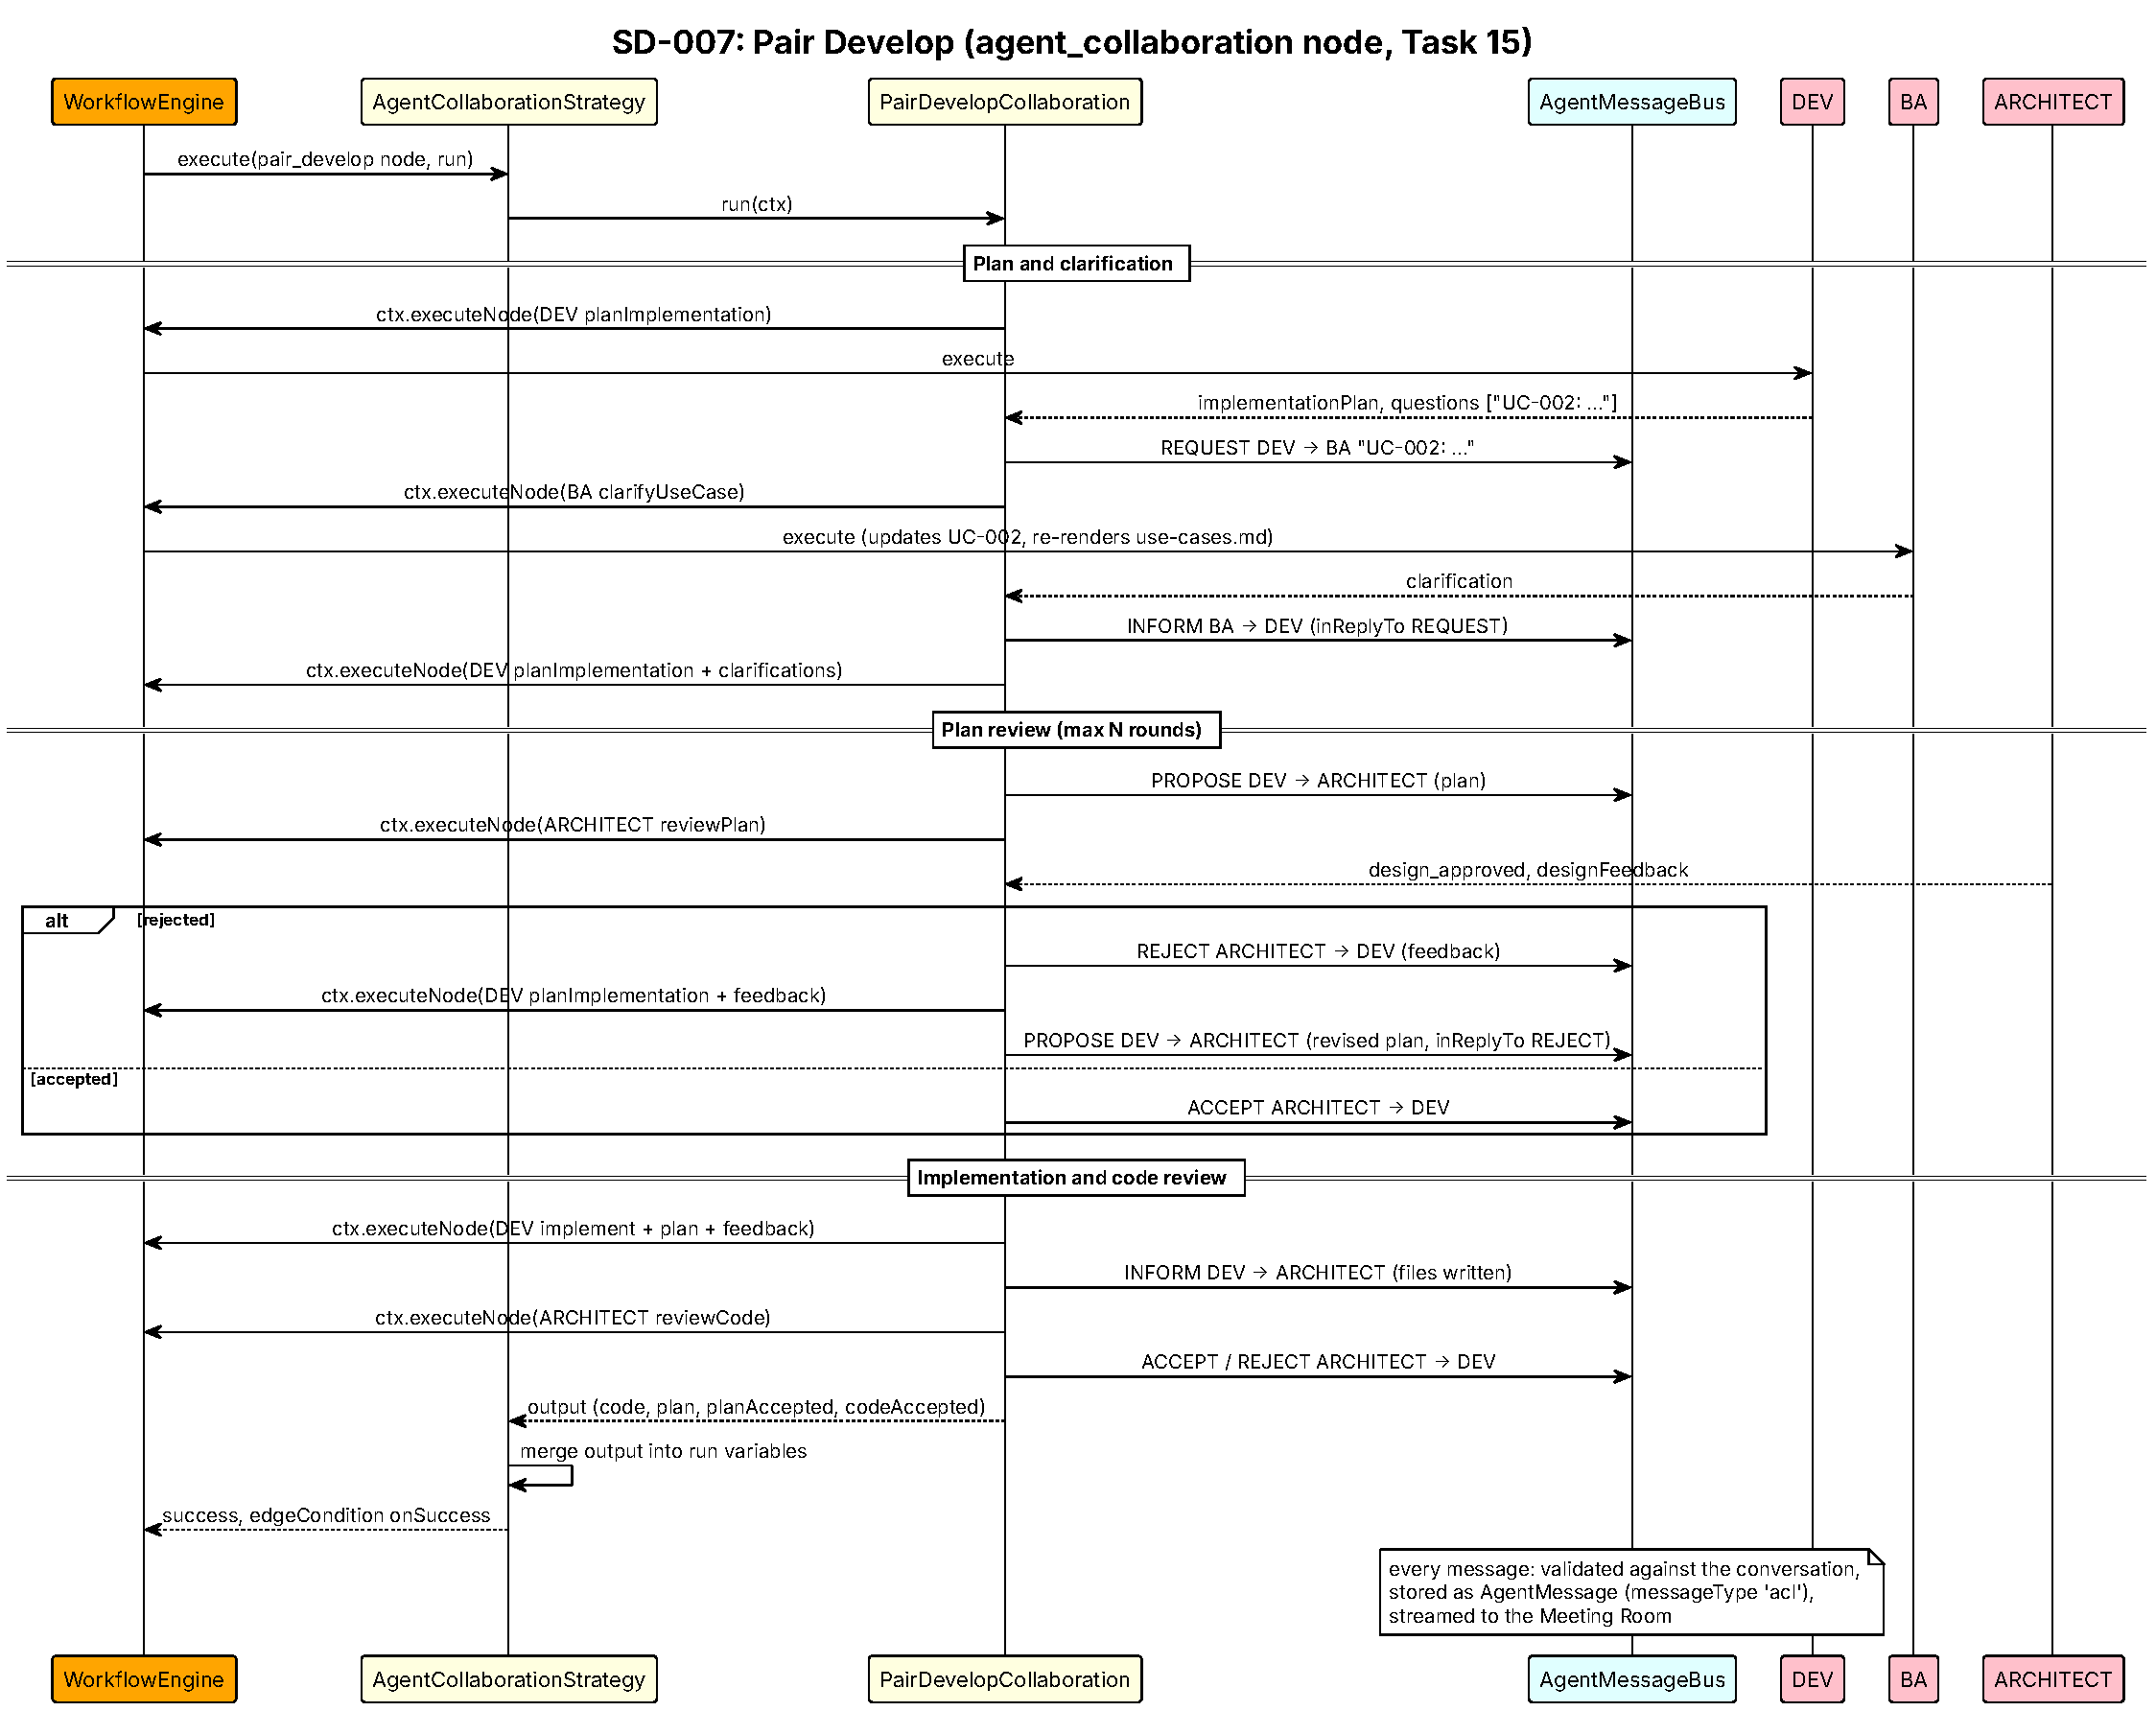
\includegraphics[width=\textwidth]{uml/SD-007-pair-develop.pdf}
\end{figure}

\begin{figure}{Sơ đồ tuần tự SD-008: thực thi quy trình con}
\label{fig:sd008}
\centering
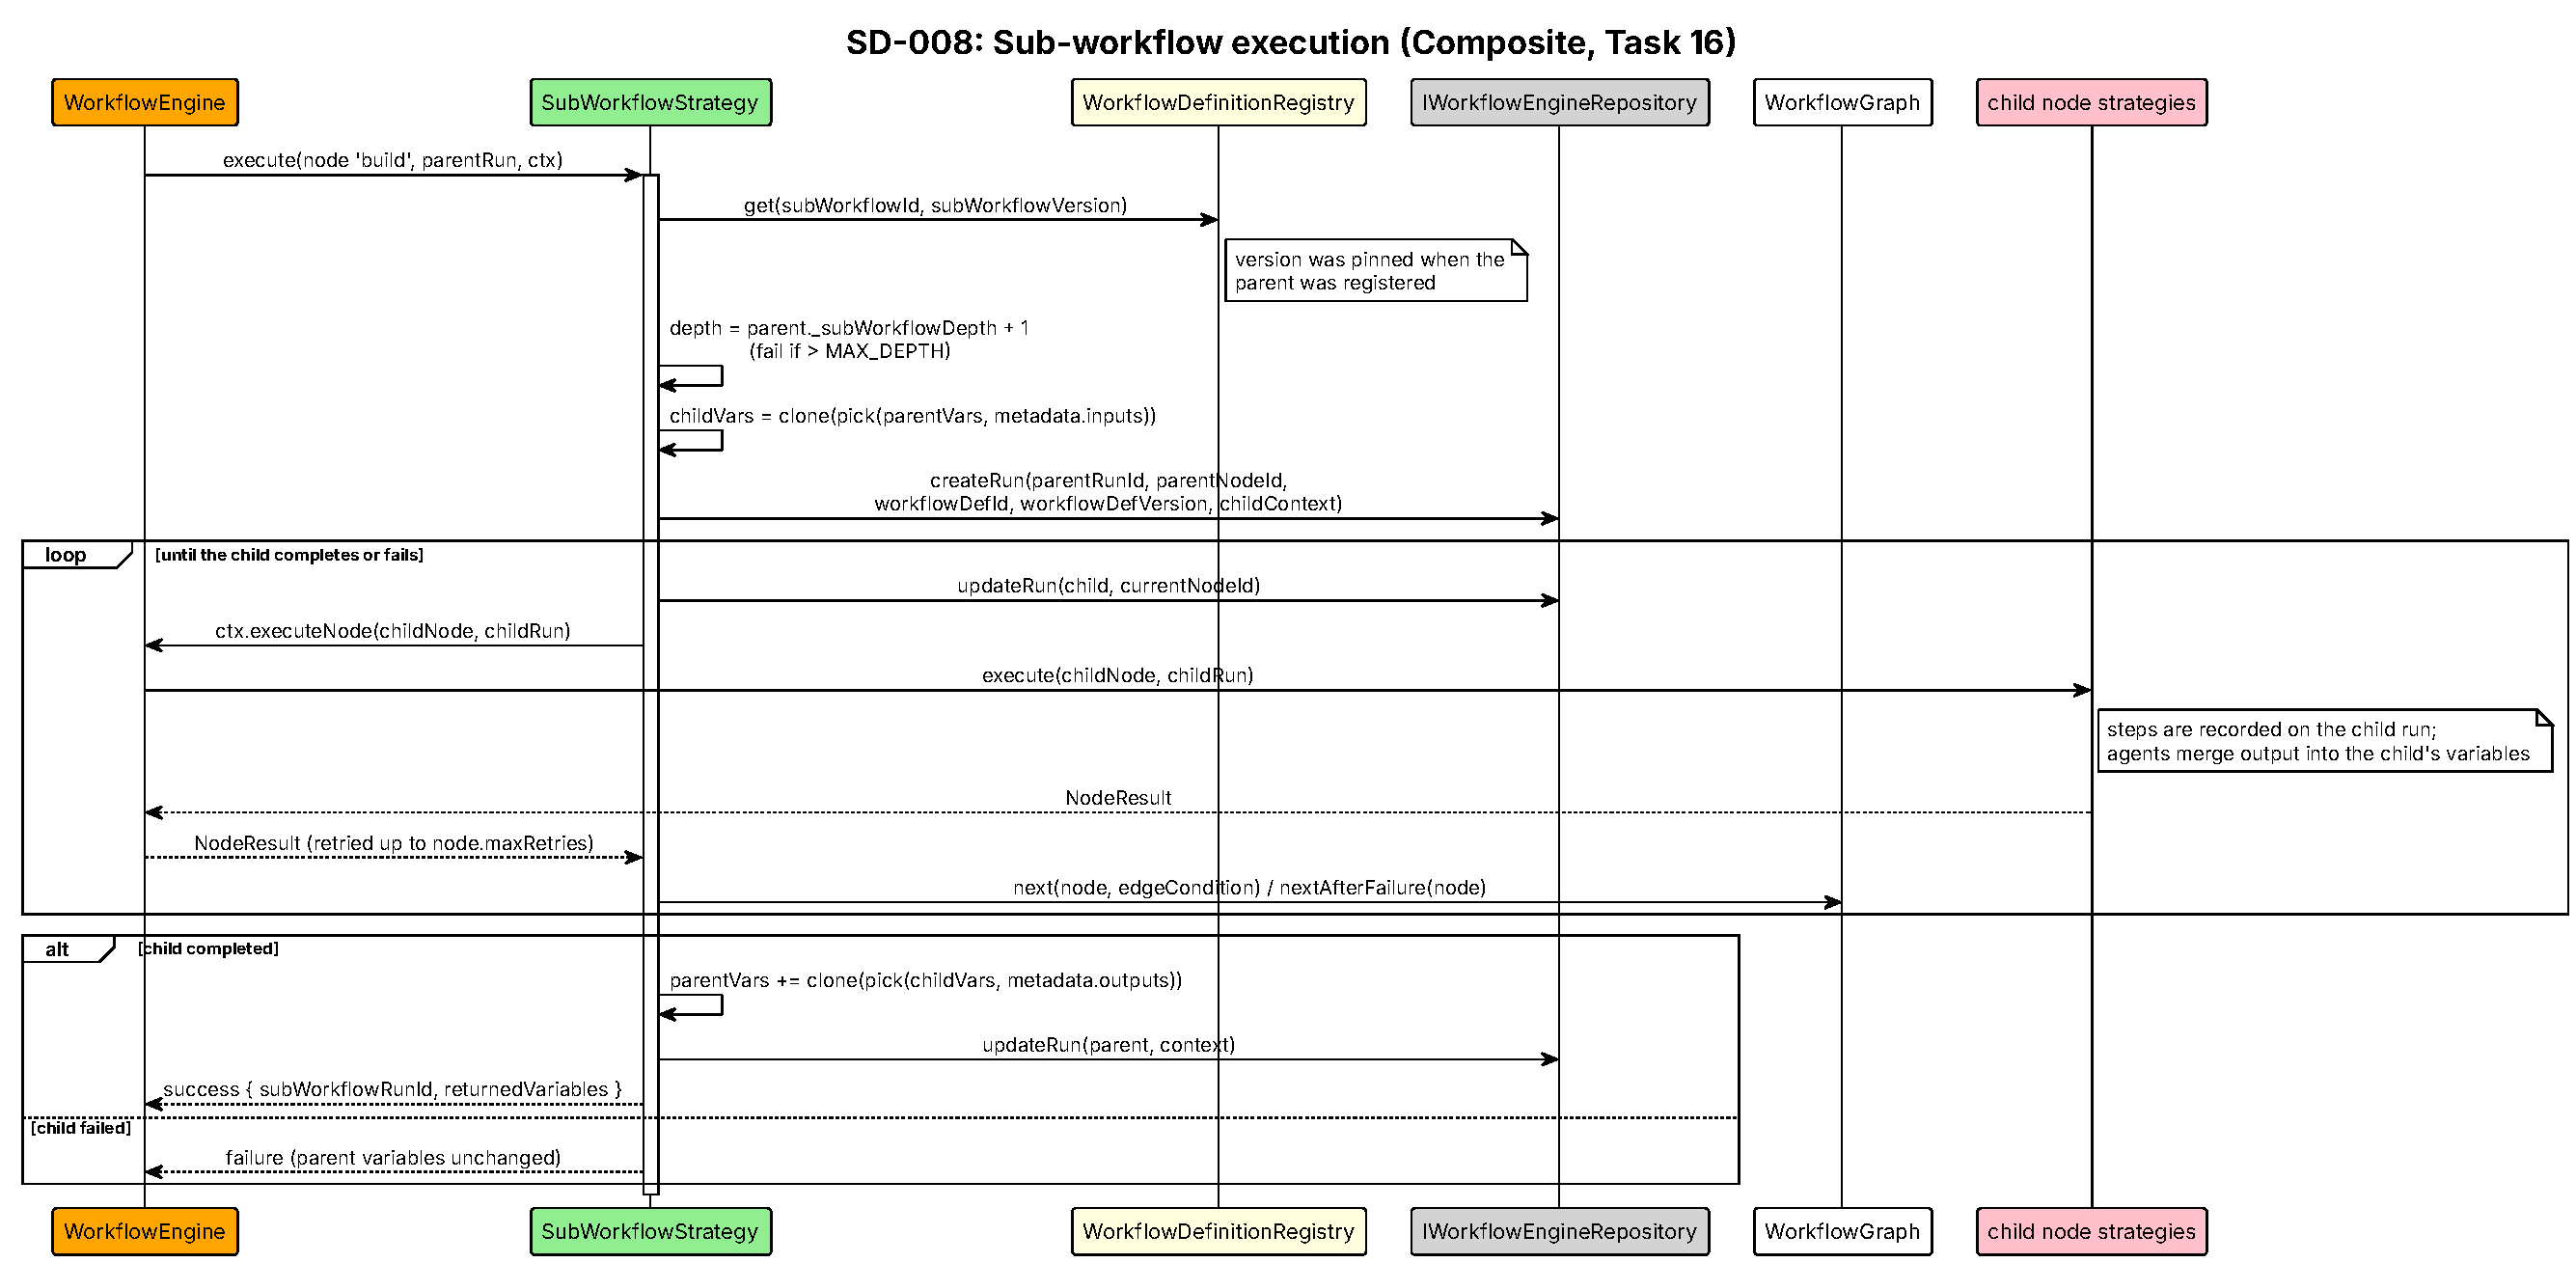
\includegraphics[width=\textwidth]{uml/SD-008-sub-workflow-execution.pdf}
\end{figure}

\begin{figure}{Sơ đồ tuần tự SD-006: ảnh chụp và khôi phục lượt chạy}
\label{fig:sd006}
\centering
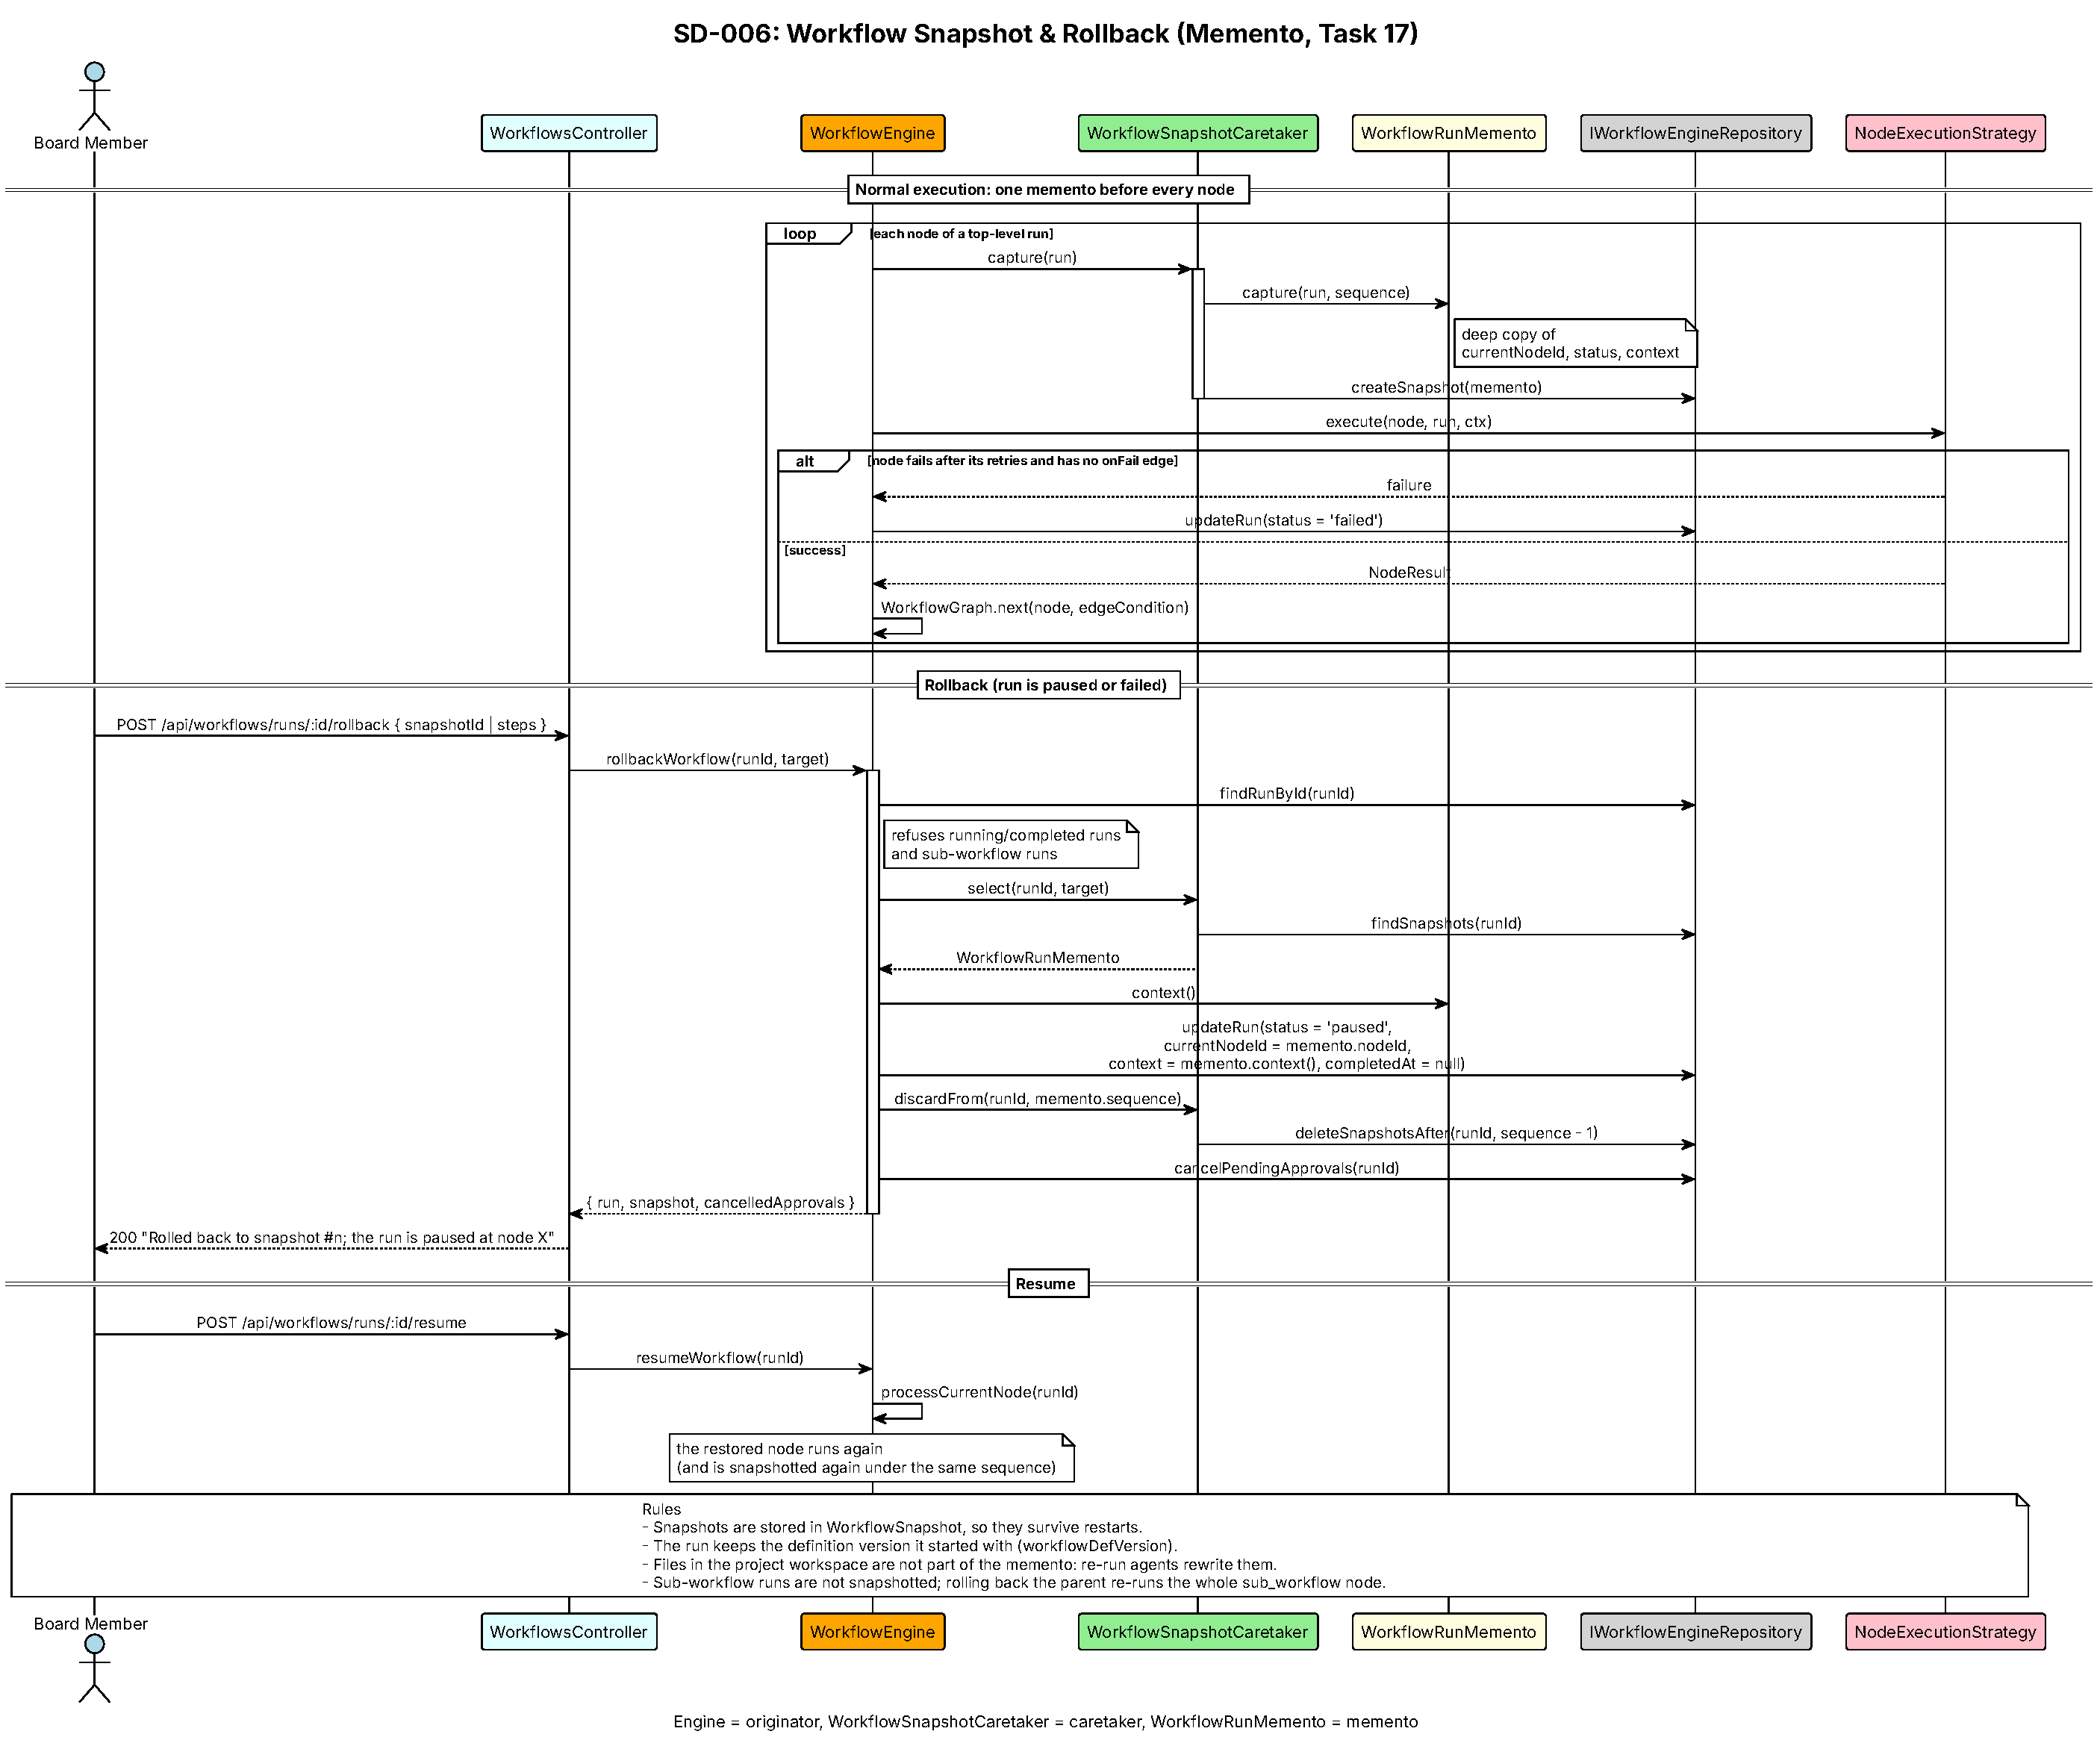
\includegraphics[width=\textwidth]{uml/SD-006-workflow-rollback.pdf}
\end{figure}

\begin{figure}{Sơ đồ tuần tự SD-009: xử lý yêu cầu có khoá API}
\label{fig:sd009}
\centering
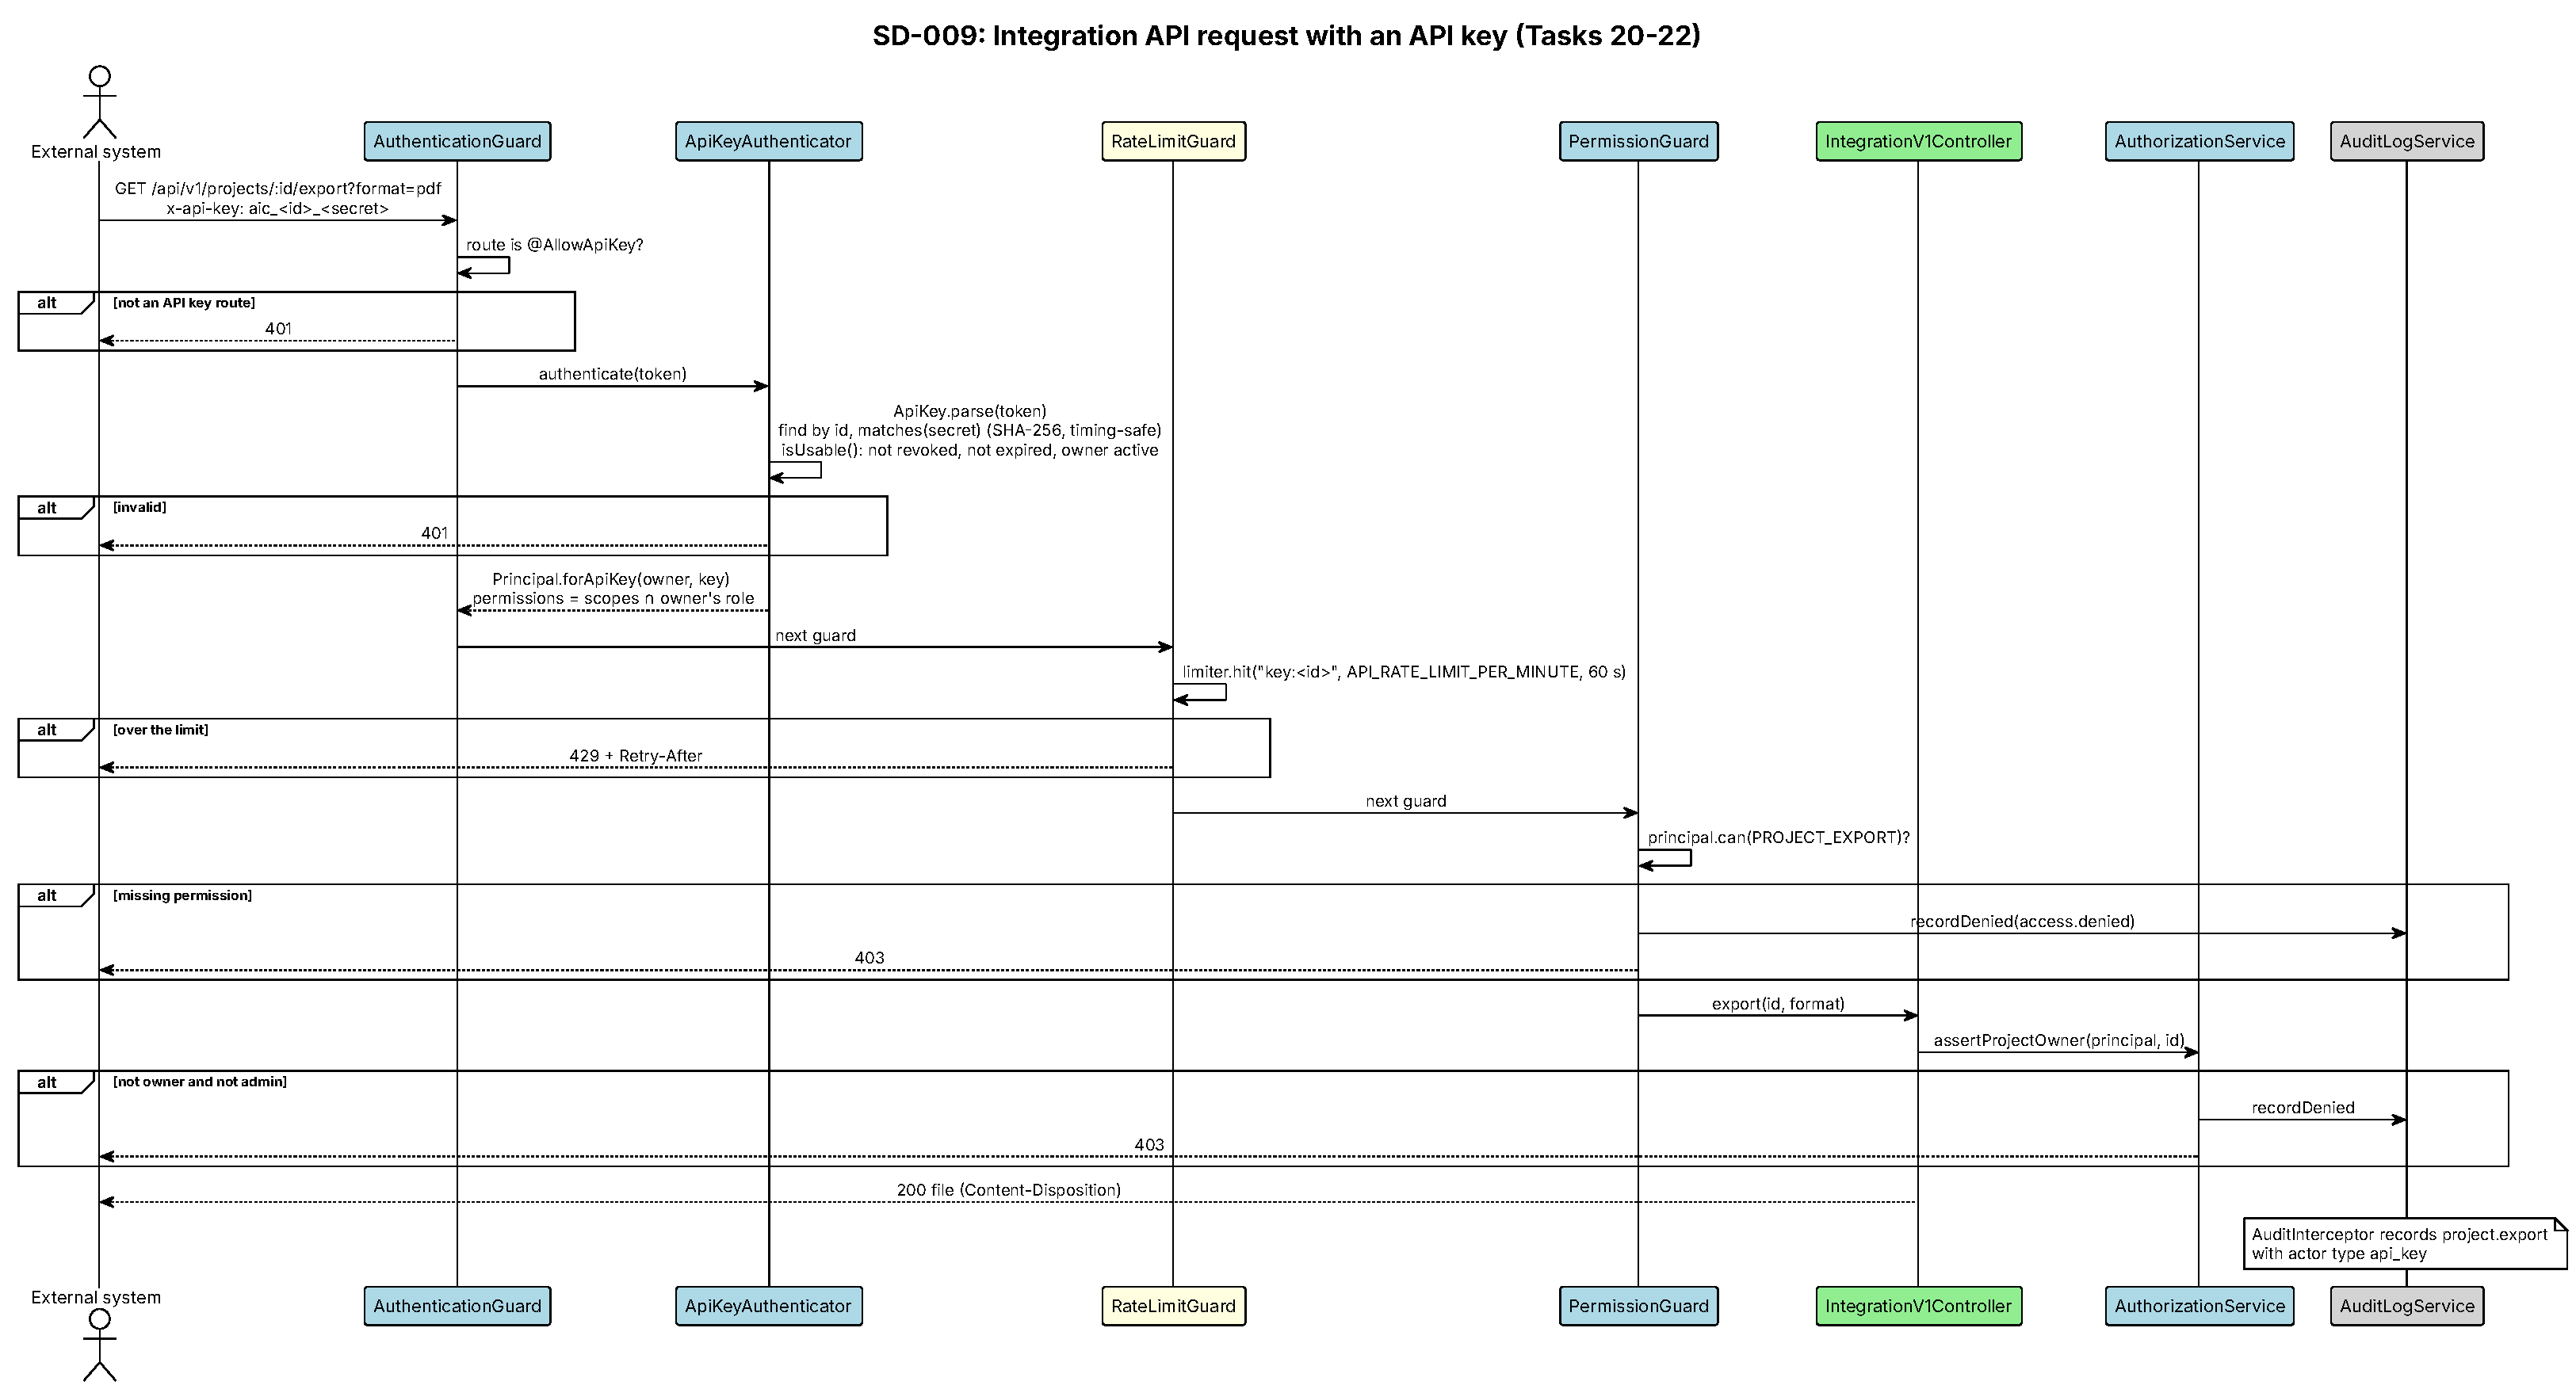
\includegraphics[width=\textwidth]{uml/SD-009-api-key-request.pdf}
\end{figure}

\begin{figure}{Sơ đồ tuần tự SD-010: gửi webhook}
\label{fig:sd010}
\centering
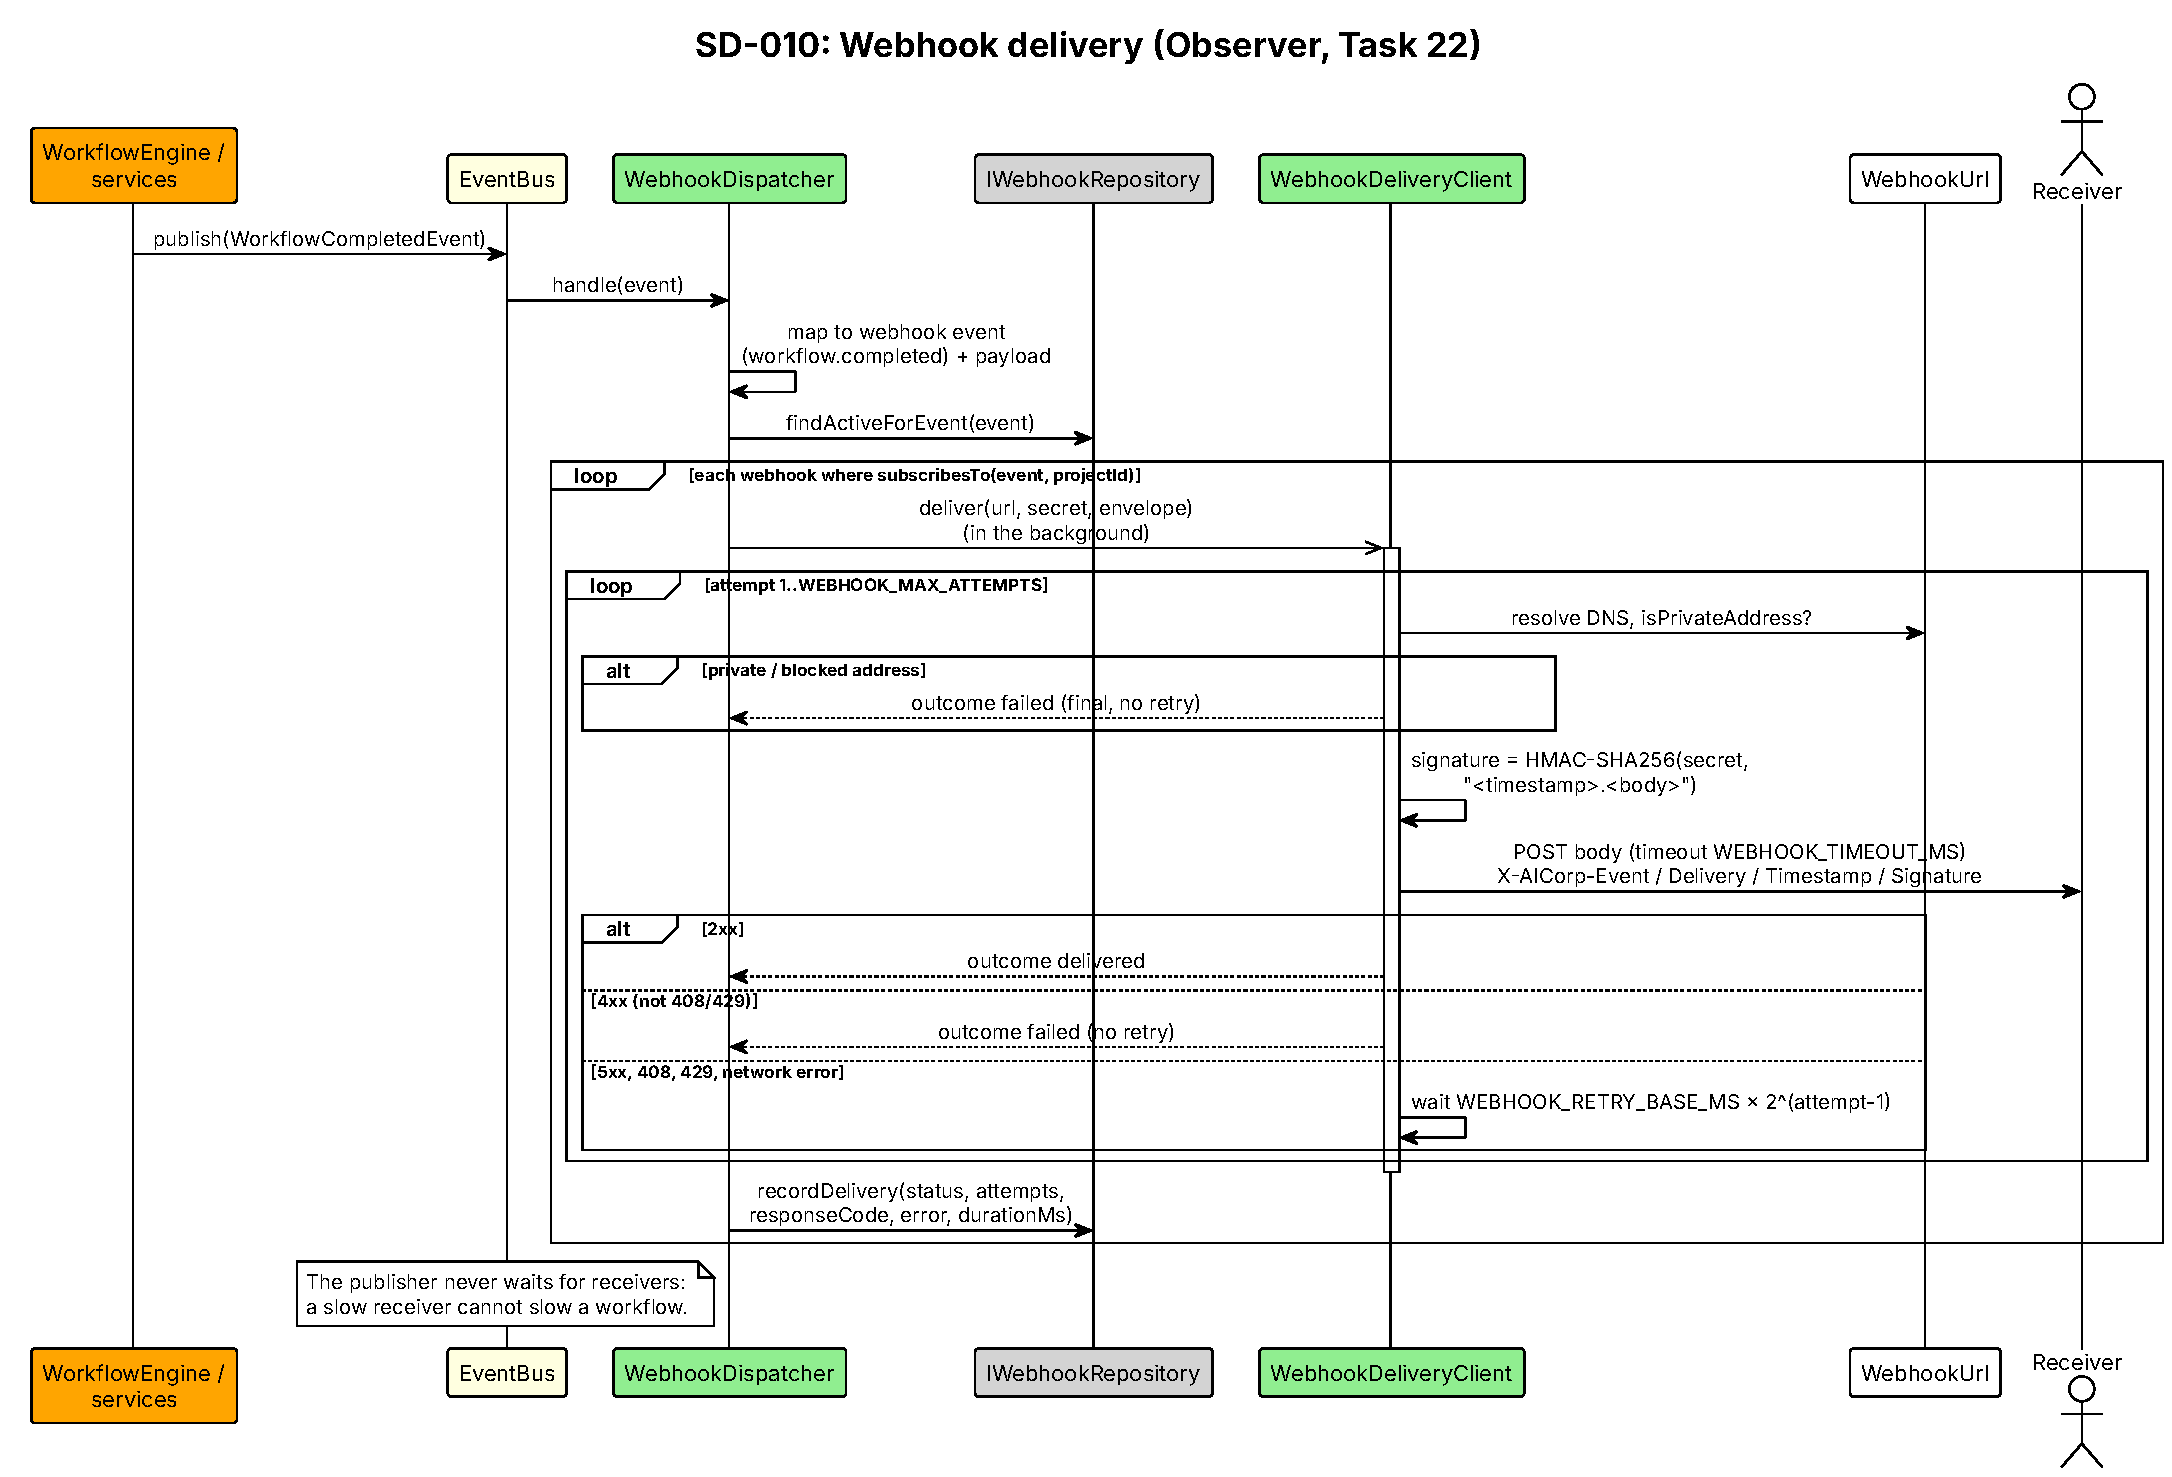
\includegraphics[width=0.9\textwidth]{uml/SD-010-webhook-delivery.pdf}
\end{figure}

\begin{figure}{Sơ đồ hoạt động AD-003: ước lượng công sức và chi phí}
\label{fig:ad003}
\centering
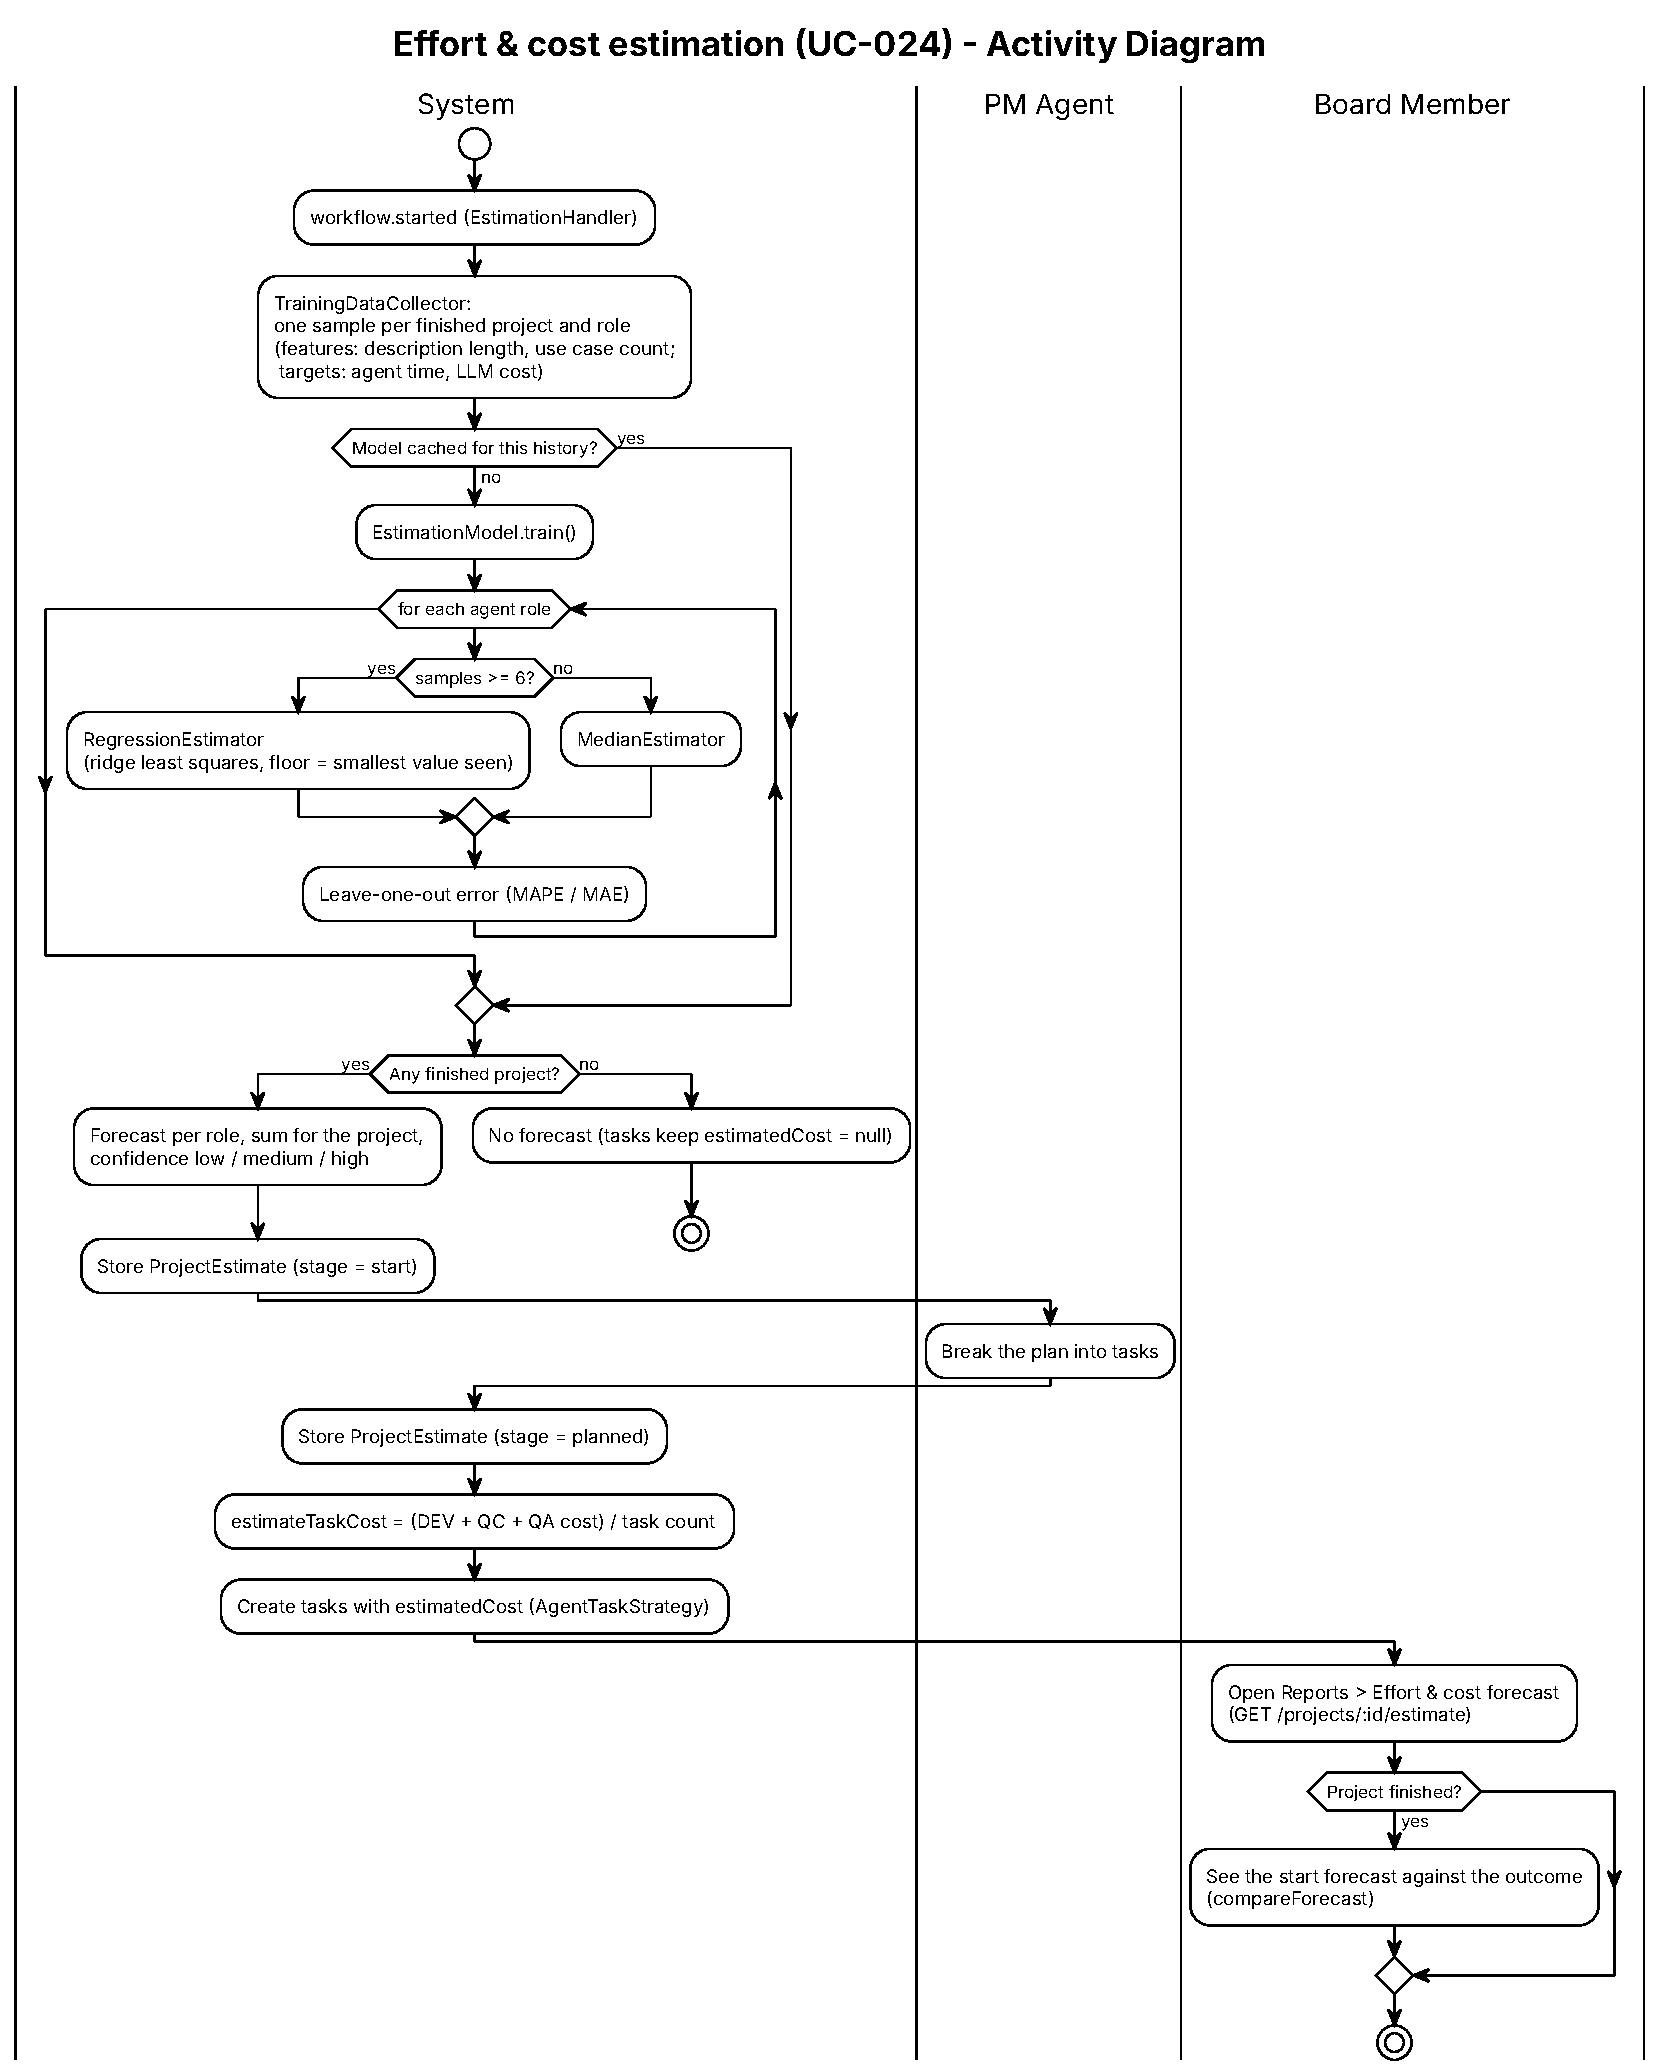
\includegraphics[height=0.55\textheight]{uml/AD-003-task-estimation-ml-pipeline.pdf}
\end{figure}

\begin{figure}{Sơ đồ hoạt động AD-004: phân tích và sửa chất lượng mã}
\label{fig:ad004}
\centering
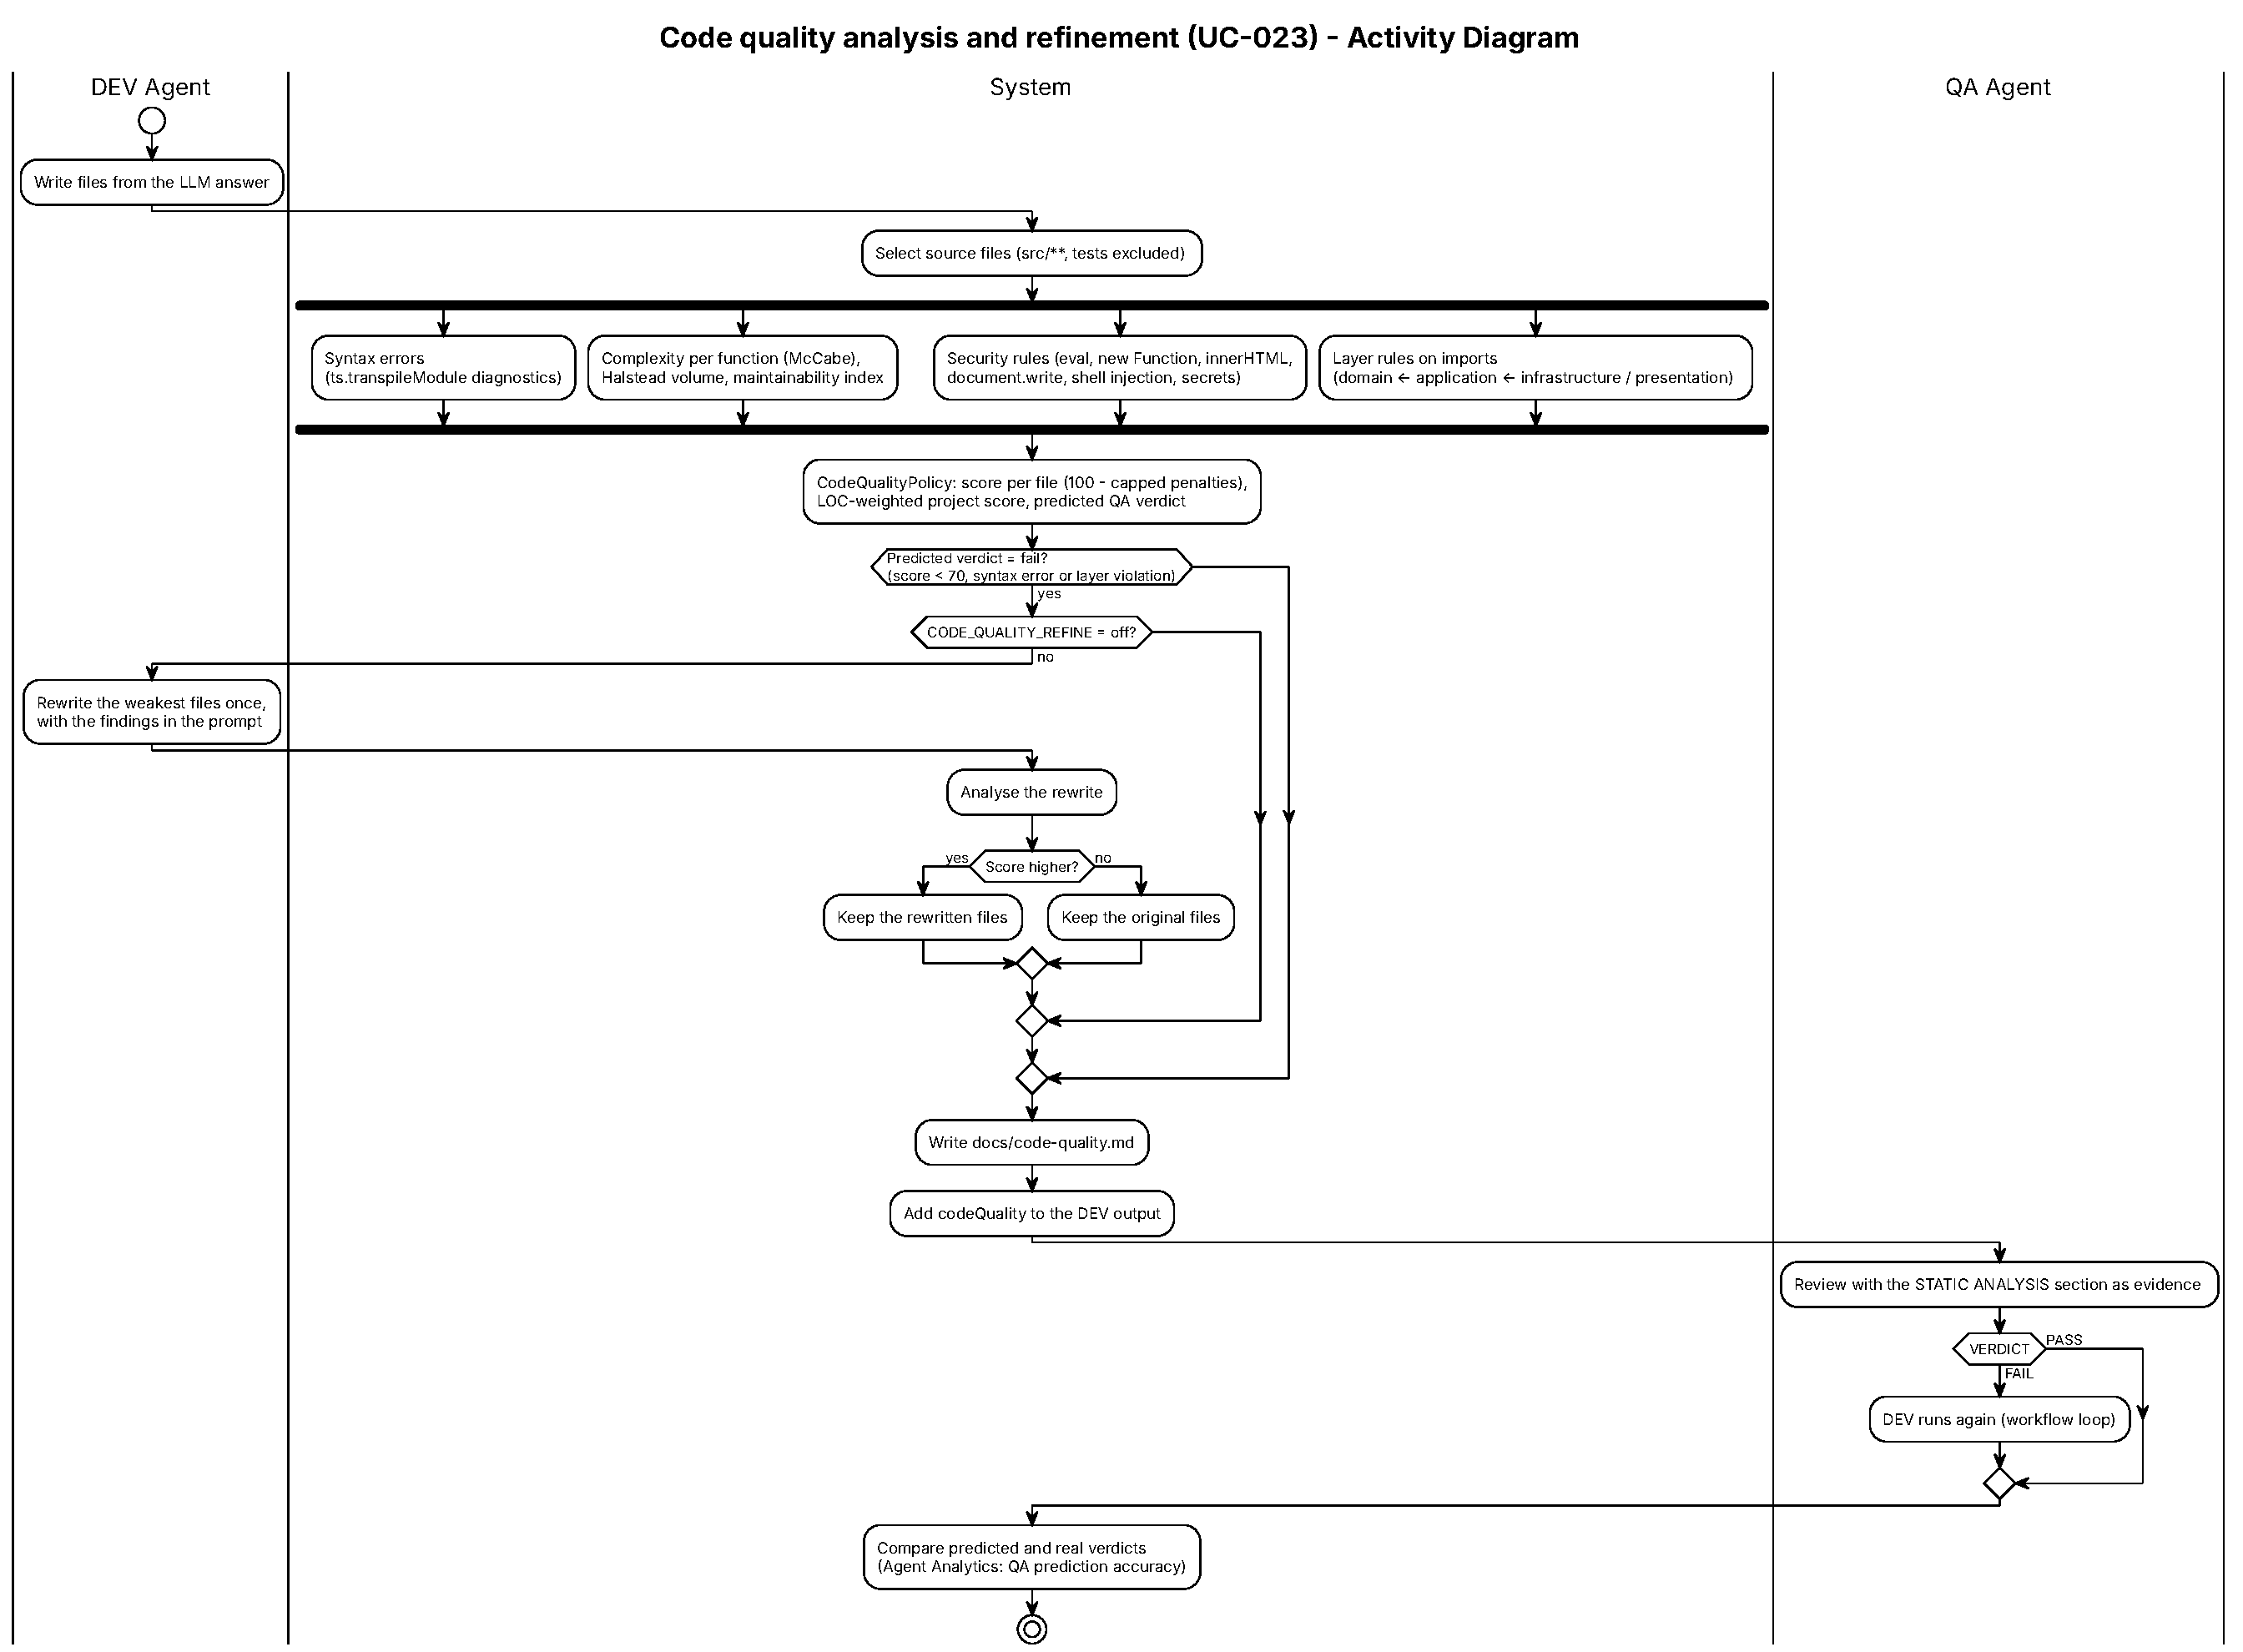
\includegraphics[width=\textwidth]{uml/AD-004-code-quality-analysis-flow.pdf}
\end{figure}

\begin{figure}{Sơ đồ máy trạng thái SM-004: phê duyệt}
\label{fig:sm004}
\centering
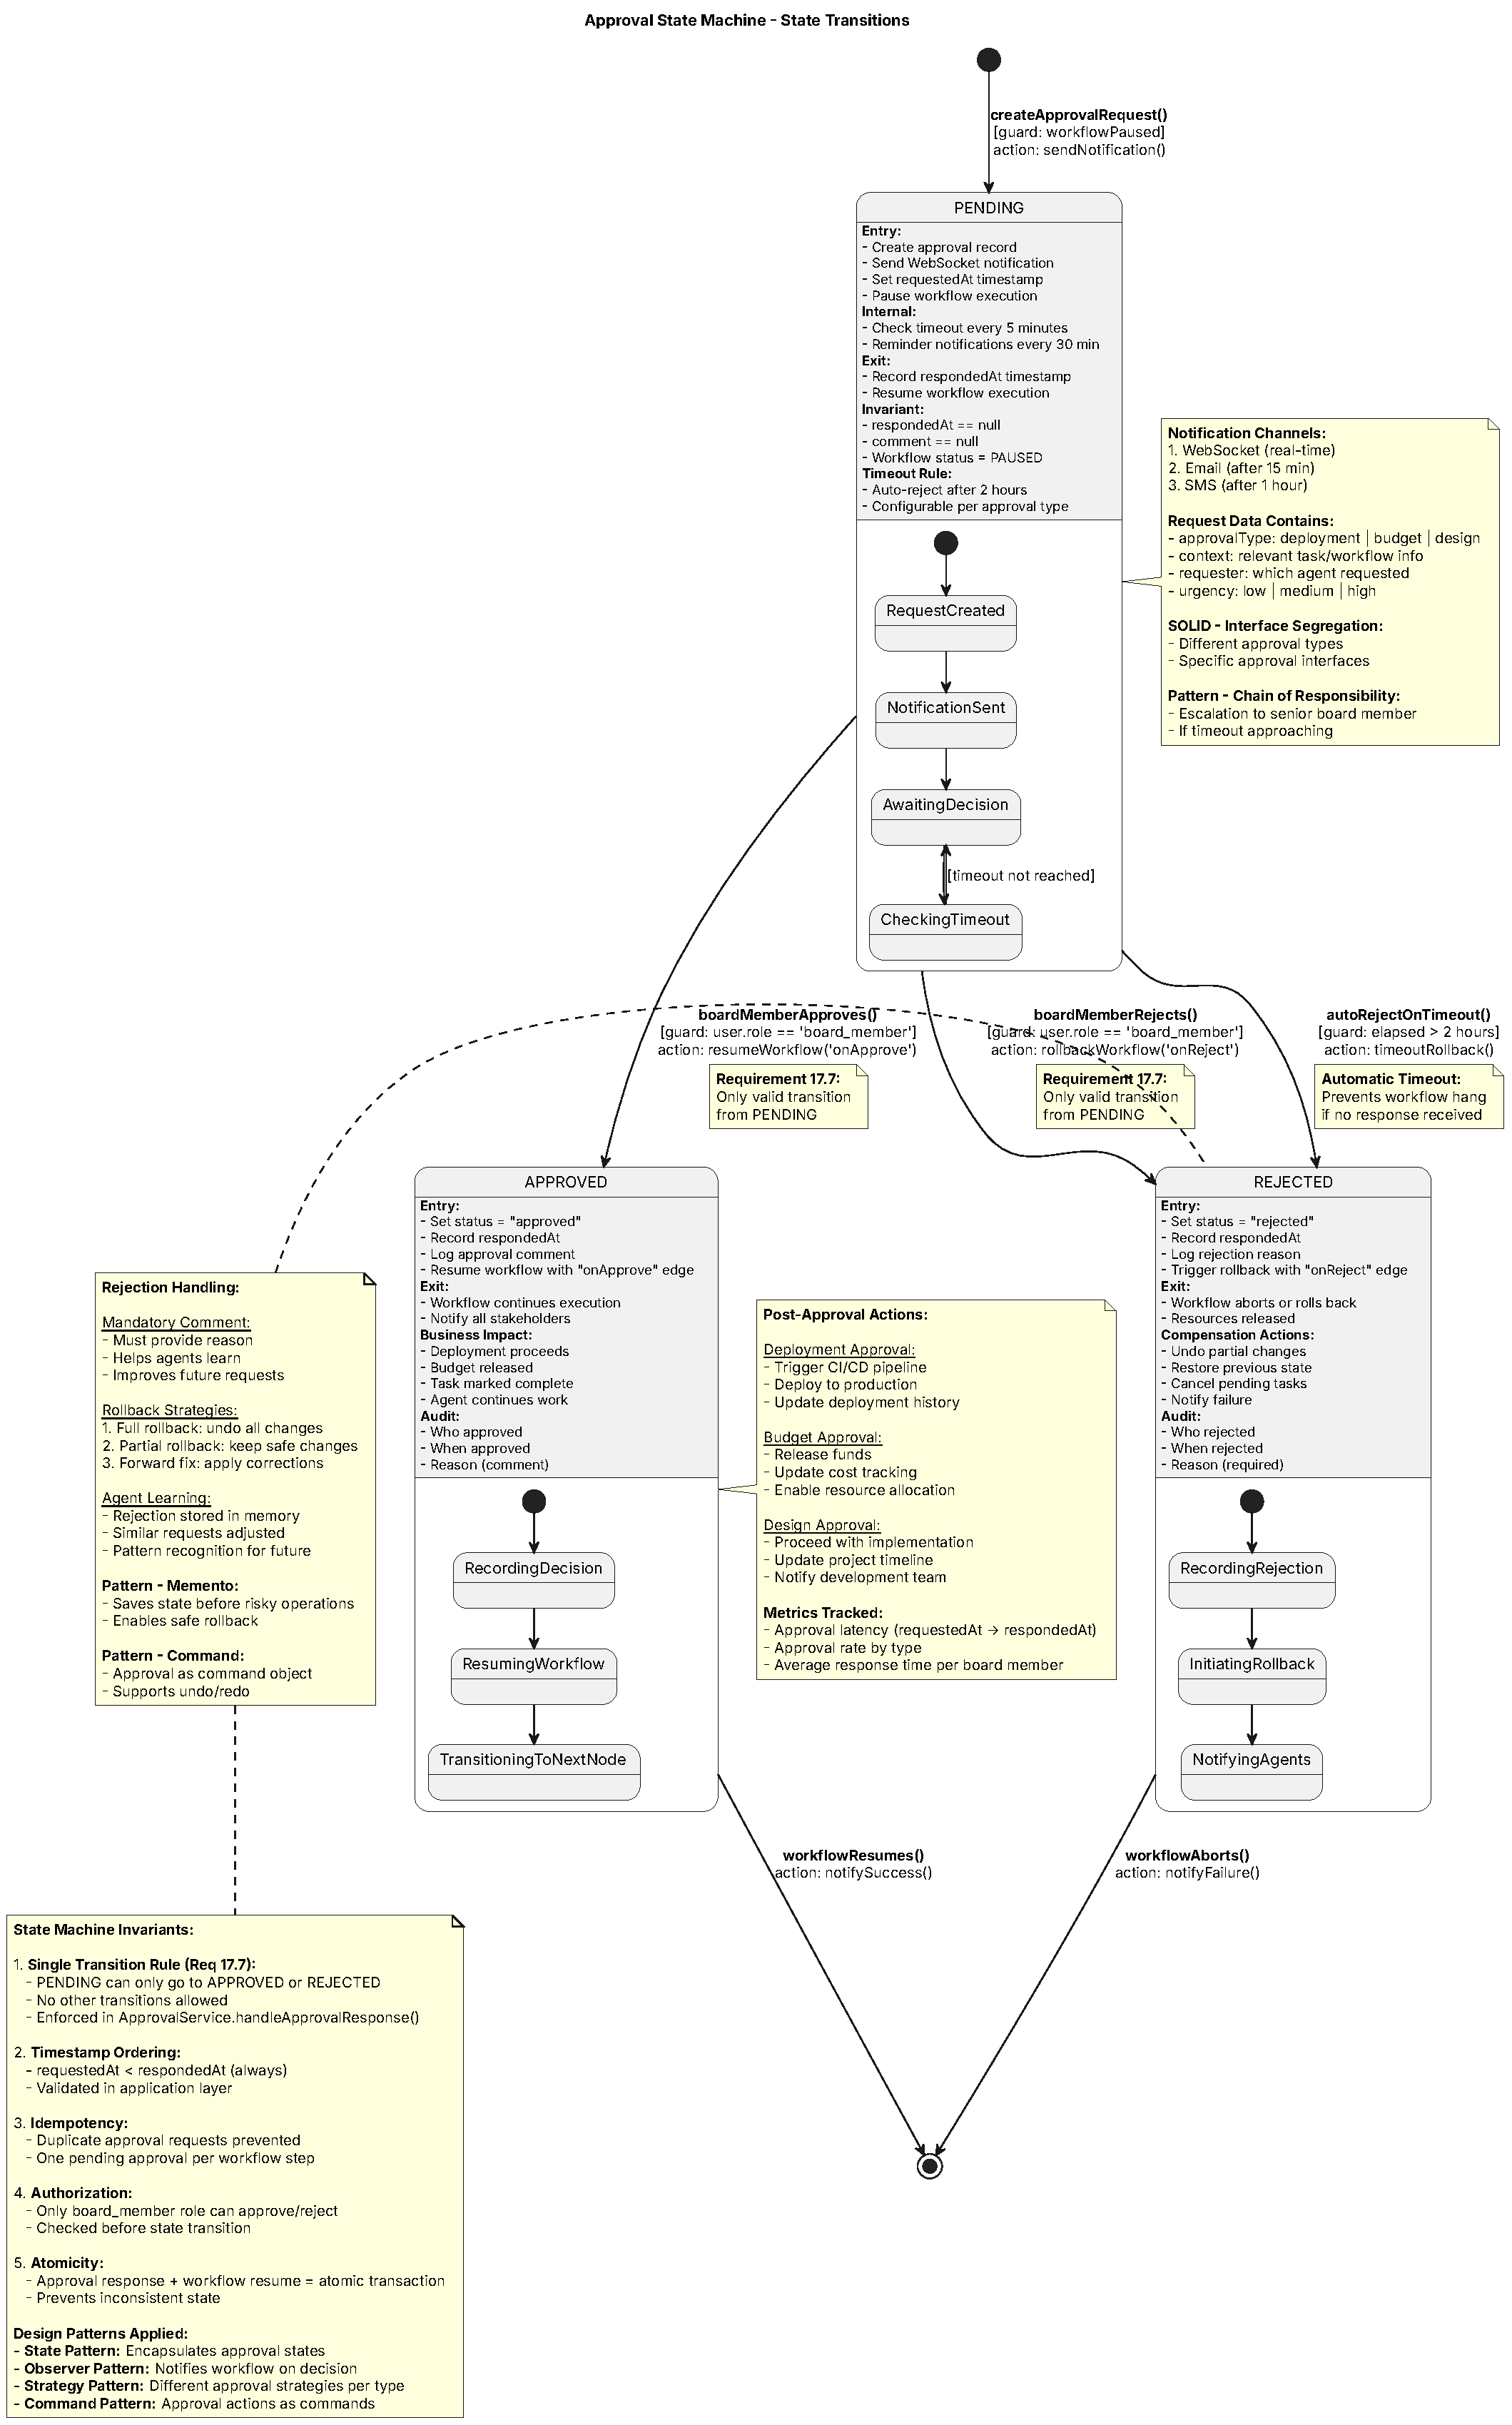
\includegraphics[height=0.5\textheight]{uml/SM-004-approval-states.pdf}
\end{figure}

\begin{figure}{Sơ đồ lớp của vòng học}
\label{fig:learning-loop}
\centering
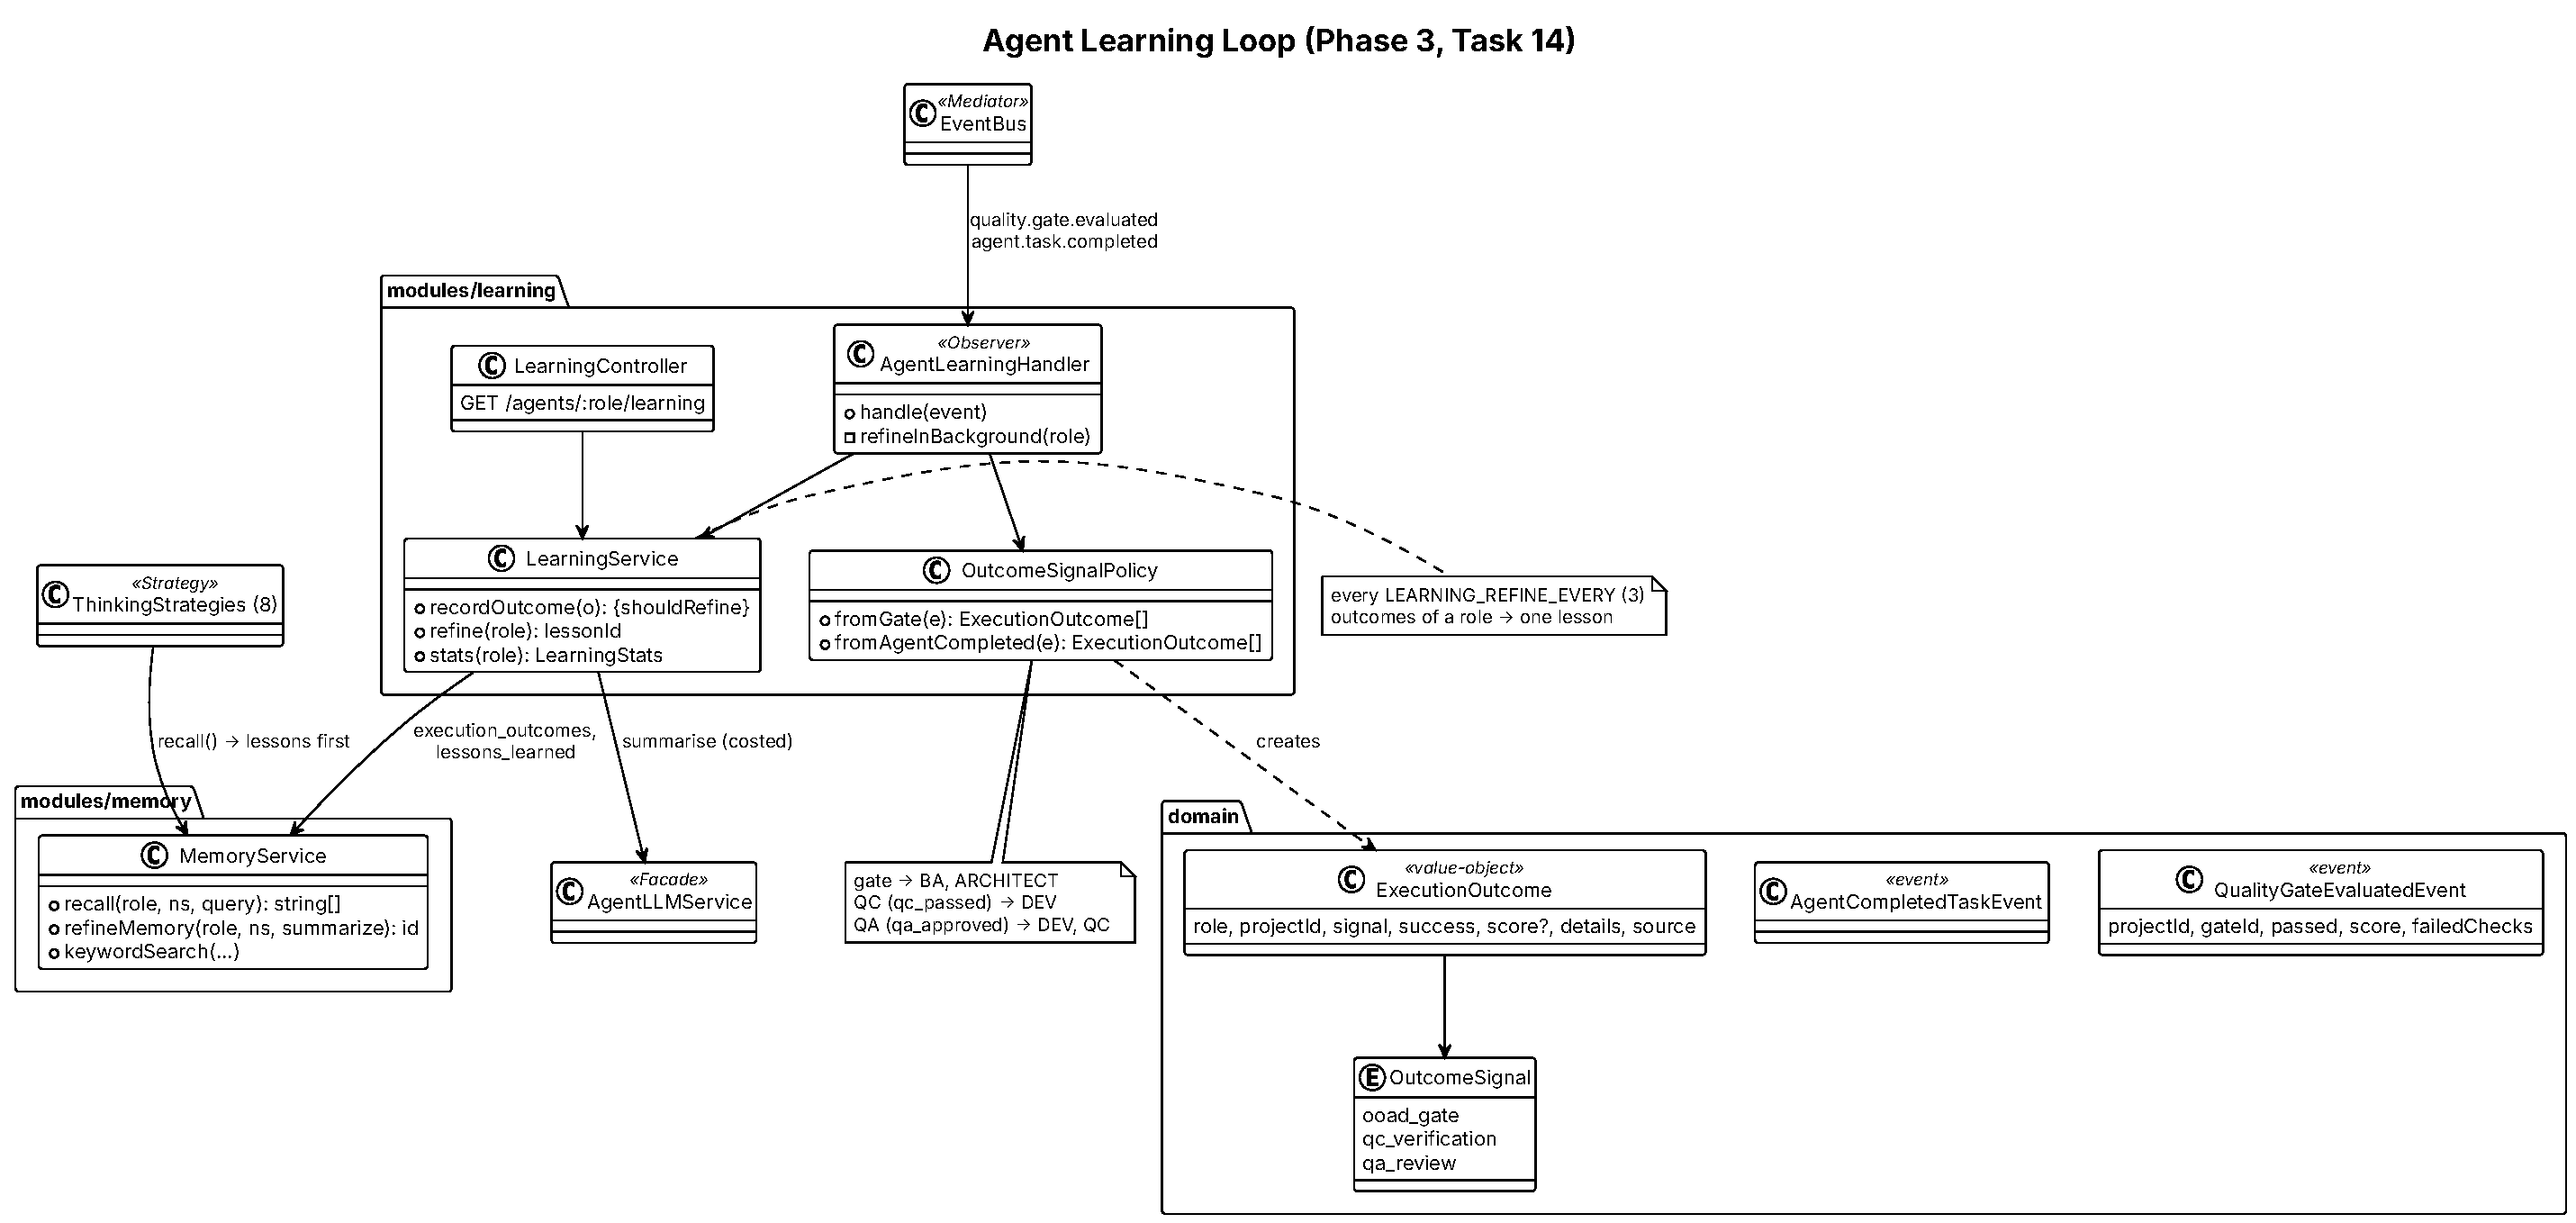
\includegraphics[width=\textwidth]{uml/learning-loop.pdf}
\end{figure}

\chapter{Giao diện lập trình}
\label{app:api}

Mọi đường dẫn đều có tiền tố \code{/api}. Trừ \code{auth/register}, \code{auth/login} và \code{health}, mọi route đều đòi JWT (giao diện web) hoặc khoá API (nhóm \code{/v1}) và được kiểm tra quyền theo vai trò. Khi \code{ENABLE_SWAGGER=true}, tài liệu OpenAPI đầy đủ có tại \code{/api/docs}.

\begin{table}{Các nhóm route của API}
\label{tab:api}
\footnotesize
\begin{tabularx}{\textwidth}{|P{2.6cm}|L|}
\hline
\textbf{Nhóm} & \textbf{Route} \\ \hline
Xác thực & \code{POST auth/register}, \code{POST auth/login}, \code{GET auth/me} \\ \hline
Dự án & \code{GET/POST projects}, \code{GET/PATCH/DELETE projects/:id} (\code{PATCH} với trạng thái tạm dừng, tiếp tục, huỷ tác động lên lượt chạy mới nhất), \code{POST projects/:id/workflow/start} \\ \hline
Công việc, mốc & \code{GET tasks}, \code{POST projects/:projectId/tasks}, \code{PATCH tasks/:id}; \code{GET/POST projects/:projectId/milestones}, \code{PATCH milestones/:id} \\ \hline
Sản phẩm dự án & \code{GET projects/:id/files}, \code{GET projects/:id/files/*}, \code{GET projects/:id/archive} (zip), \code{GET projects/:id/quality-gates} \\ \hline
Phê duyệt & \code{GET approvals}, \code{POST approvals/:id/approve}, \code{POST approvals/:id/reject} (bắt buộc lý do; 409 nếu đã trả lời) \\ \hline
Quy trình & \code{GET workflows/templates}, \code{POST workflows/templates/:templateId/preview}, \code{GET workflows/definitions[/:definitionId]}, \code{GET workflows/runs/:runId}, \code{GET workflows/runs/:runId/snapshots}, \code{POST workflows/runs/:runId/rollback}, \code{POST workflows/runs/:runId/pause}, \code{POST workflows/runs/:runId/resume} \\ \hline
Mô hình LLM & \code{GET models}, \code{GET models/available}, \code{PATCH models/:role} (kèm \code{providerId}) \\ \hline
Nhà cung cấp LLM & \code{GET/POST llm-providers}, \code{GET llm-providers/kinds}, \code{PATCH/DELETE llm-providers/:id}, \code{POST llm-providers/:id/test}, \code{GET llm-providers/:id/remote-models}, \code{POST llm-providers/:id/models}, \code{PATCH/DELETE llm-providers/:id/models/:modelId} \\ \hline
Chi phí, báo cáo, xuất & \code{GET cost/summary}, \code{GET reports/projects/:id/cost}, \code{GET reports/performance}, \code{POST reports/weekly/run}, \code{GET projects/:id/export?format=json|csv|pdf} \\ \hline
Phân tích, dự báo, chất lượng & \code{GET analytics/agents}, \code{GET agents/:role/learning}, \code{GET projects/:id/estimate}, \code{GET analytics/estimation}, \code{GET projects/:id/code-quality}, \code{GET ooad-metrics/dashboard}, \code{GET ooad-metrics/project/:id}, \code{GET ooad-metrics/leaderboard} \\ \hline
Người dùng, kiểm toán & \code{GET users}, \code{GET users/roles}, \code{PATCH users/:id/role}, \code{PATCH users/:id/active}; \code{GET audit}, \code{GET audit/export}, \code{GET audit/anomalies} \\ \hline
Tích hợp (quản trị) & \code{GET integrations/events}, \code{GET/POST integrations/api-keys}, \code{DELETE integrations/api-keys/:id}, \code{GET/POST integrations/webhooks}, \code{DELETE integrations/webhooks/:id}, \code{POST integrations/webhooks/:id/test}, \code{GET integrations/webhooks/:id/deliveries} \\ \hline
API công khai (khoá API) & \code{GET/POST v1/projects}, \code{GET v1/projects/:id/status}, \code{GET v1/projects/:id/reports/cost}, \code{GET v1/projects/:id/export}, \code{GET/POST v1/webhooks}, \code{DELETE v1/webhooks/:id} \\ \hline
Sức khoẻ & \code{GET health} (503 khi cơ sở dữ liệu ngừng), \code{GET health/live} \\ \hline
\end{tabularx}
\end{table}

Về WebSocket (Socket.IO, xác thực bằng JWT lúc kết nối): máy khách gửi \code{subscribe_project} để nhận \code{project_event} của một dự án; máy chủ phát thêm \code{system_event} (trạng thái tác tử) và \code{user_event}. Thông điệp \code{human:approval_response} bị từ chối; phê duyệt chỉ đi qua REST.

\chapter{Tái tạo số liệu kiểm thử và hiệu năng}
\label{app:tai-tao}

\section{Kiểm thử tự động}

\begin{Verbatim}
pnpm install
cd apps/api && npx jest              # 50 bộ, 707 đạt, 15 bỏ qua
cd apps/api && npm run test:cov      # độ bao phủ, lỗi nếu dưới ngưỡng
cd apps/web && npx vitest run && npx tsc --noEmit
\end{Verbatim}

\section{Kiểm thử đầu cuối}

Mỗi lần chạy có script, kết quả và ảnh chụp màn hình lưu trong một thư mục \code{docs/*-e2e/} của kho mã, kèm README ghi môi trường và câu lệnh. Script in một dòng cho mỗi kiểm tra và trả mã 1 nếu có kiểm tra hỏng. Môi trường chung gồm PostgreSQL 16 có pgvector, Redis 7, API build ở chế độ production và LLM kịch bản \code{scripts/demo/demo-llm.cjs} (tương thích OpenAI, cổng 20128). Lần chạy triển khai đi qua nginx với cấu hình giống \code{apps/web/nginx.conf}.

\begin{table}{Script của các lần chạy đầu cuối}
\label{tab:e2e-script}
\small
\begin{tabularx}{\textwidth}{|L|P{6.2cm}|r|}
\hline
\textbf{Lần chạy} & \textbf{Script} & \textbf{Kiểm tra} \\ \hline
Triển khai và trình diễn & \code{docs/phase7-e2e/e2e.mjs} sau \code{scripts/demo/seed-demo.mjs} & 24 \\ \hline
Phân tích, dự báo, chất lượng mã & \code{docs/phase6-e2e/e2e.mjs} & 21 \\ \hline
Bảo mật, kiểm toán, tích hợp & \code{docs/phase5-e2e/e2e.mjs} & 44 \\ \hline
Bộ máy quy trình & \code{docs/phase4-e2e/e2e.mjs} & theo kịch bản \\ \hline
\end{tabularx}
\end{table}

\section{LLM kịch bản}

Máy chủ trả lời theo vai trò và nội dung lời nhắc. Bảng~\ref{tab:kich-ban} liệt kê các quy tắc ảnh hưởng tới kết quả đánh giá.

\begin{table}{Quy tắc của LLM kịch bản}
\label{tab:kich-ban}
\small
\begin{tabularx}{\textwidth}{|P{5cm}|L|}
\hline
\textbf{Điều kiện} & \textbf{Câu trả lời} \\ \hline
Tên dự án bắt đầu bằng ``Legacy'' & Mã lần đầu của DEV nhập hạ tầng từ miền, có khoá viết cứng, \code{eval} và phương thức dài, còn bản sửa thì sạch \\ \hline
Tên dự án bắt đầu bằng ``Unsafe'' & Mã có \code{eval}, QA trả FAIL lần đầu và PASS lần hai \\ \hline
Mô hình của Marketing bị đánh dấu ngừng hoạt động & Lỗi 503, dùng để kiểm tra phát hiện bất thường \\ \hline
Mọi lời gọi & Độ trễ 20~ms cộng 1~ms cho mỗi 25 ký tự lời nhắc, số token theo độ dài, giá theo tên mô hình \\ \hline
\end{tabularx}
\end{table}

Script \code{scripts/demo/seed-demo.mjs} tạo hai tài khoản (thành viên hội đồng quản trị và người xem) cùng năm dự án trình diễn. Chạy lại script bao nhiêu lần cũng được, lần sau không tạo bản trùng. Các ảnh giao diện Ant Design 6 trong khoá luận được chụp trên đúng bộ dữ liệu này, bằng Playwright ở khung 1440×900 điểm ảnh và chế độ sáng. Riêng ảnh Phòng họp được chụp trong lúc một dự án thứ sáu đang chạy, vì Phòng họp chỉ hiện các trao đổi đang diễn ra.

\section{Kiểm thử tải}

Script \code{scripts/perf/load-test.mjs} không cần thư viện ngoài, còn ngân sách nằm trong \code{scripts/perf/budgets.json}.

\begin{Verbatim}
node scripts/perf/load-test.mjs --api http://localhost:3000/api \
     --users 20 --duration 30 --create-every 0
node scripts/perf/load-test.mjs --users 20 --duration 30 --create-every 10
node scripts/perf/load-test.mjs --users 50 --duration 30 --create-every 25
\end{Verbatim}

Bảng~\ref{tab:tai-chi-tiet} là kết quả chi tiết với 20 người dùng chỉ đọc: 30 giây, 18\,154 yêu cầu, 604,8 yêu cầu mỗi giây, 0\% lỗi, cơ sở dữ liệu bắt đầu từ 5 dự án trình diễn.

\begin{table}{Thời gian phản hồi theo endpoint, 20 người dùng chỉ đọc}
\label{tab:tai-chi-tiet}
\small
\begin{tabular}{|l|r|r|r|r|c|}
\hline
\textbf{Endpoint} & \textbf{Số yêu cầu} & \textbf{p50} & \textbf{p95} & \textbf{p99} & \textbf{Ngân sách (ms)} \\ \hline
\code{GET /analytics/agents} & 1\,832 & 30 & 44 & 52 & 300/1500/3000 \\ \hline
\code{GET /health} & 911 & 54 & 84 & 97 & 100/500/1000 \\ \hline
\code{GET /projects} & 4\,472 & 28 & 42 & 51 & 100/500/1000 \\ \hline
\code{GET /projects/:id} & 3\,674 & 31 & 46 & 54 & 100/500/1000 \\ \hline
\code{GET /projects/:id/code-quality} & 1\,794 & 20 & 33 & 44 & 300/1500/3000 \\ \hline
\code{GET /projects/:id/estimate} & 1\,838 & 47 & 66 & 78 & 300/1500/3000 \\ \hline
\code{GET /reports/projects/:id/cost} & 1\,751 & 36 & 51 & 59 & 100/500/1000 \\ \hline
\code{GET /tasks?projectId} & 1\,882 & 27 & 41 & 51 & 100/500/1000 \\ \hline
\end{tabular}
\end{table}

Bảng~\ref{tab:loi-hieu-nang} là ba lỗi hiệu năng tìm được ở lần đo trước (cơ sở dữ liệu khoảng 120 dự án) và tác dụng của bản sửa. Trong lần đo đó, sau khi sửa, thông lượng ở kịch bản bão hoà tăng từ 98,8 lên 178,3 yêu cầu mỗi giây.

\begin{table}{Ba lỗi hiệu năng và kết quả sau khi sửa}
\label{tab:loi-hieu-nang}
\small
\begin{tabularx}{\textwidth}{|P{4.2cm}|L|P{2.8cm}|}
\hline
\textbf{Lỗi} & \textbf{Cách sửa} & \textbf{Kết quả} \\ \hline
Endpoint chất lượng mã phân tích lại mọi tệp ở mỗi yêu cầu & Lưu kết quả theo mã băm nội dung tệp và theo dự án trong 30~s, DEV xoá bộ đệm khi ghi lại mã, đọc tệp song song & p50 từ 3\,116 xuống 196~ms \\ \hline
Danh sách dự án tải JSON ngữ cảnh lượt chạy rồi bỏ đi & Repository chỉ chọn các cột DTO cần & 46 xuống 9~ms (1 người dùng) \\ \hline
Chi tiết dự án chạy bốn truy vấn độc lập tuần tự & Chạy song song & 16 xuống 9~ms (1 người dùng) \\ \hline
\end{tabularx}
\end{table}

Dữ liệu thời gian theo bước tác tử lấy từ trường \code{durationMs} của các bước trong lượt chạy, đọc qua \code{GET /api/workflows/runs/:runId}. Các lượt chạy của lần kiểm thử triển khai được lưu trong \code{docs/phase7-e2e/out/}.

\chapter{Hướng dẫn cài đặt và sử dụng}
\label{app:huong-dan}

\section{Cài đặt bằng Docker}

\begin{Verbatim}
cp .env.production.example .env.production
# Điền POSTGRES_PASSWORD, JWT_SECRET (openssl rand -hex 32),
# CORS_ORIGIN, NINE_ROUTER_URL, NINE_ROUTER_API_KEY,
# SEED_ADMIN_EMAIL, SEED_ADMIN_PASSWORD (tối thiểu 12 ký tự),
# LLM_SECRET_KEY. Tuỳ chọn: SIGNUP_ROLE, ALLOW_REGISTRATION,
# JWT_EXPIRATION (giây, mặc định 8 giờ)
docker compose -f docker-compose.prod.yml \
  --env-file .env.production up -d --build
\end{Verbatim}

Giao diện web chạy ở \code{http://localhost:8080}, đổi cổng bằng \code{WEB_PORT}. Lần khởi động đầu chạy migration và tạo tài khoản quản trị, sau đó nên đặt \code{SEED_ON_START=false}. API từ chối khởi động nếu còn giá trị mẫu \code{CHANGE_ME}, thiếu \code{JWT_SECRET} hoặc \code{CORS_ORIGIN}, hoặc khoá JWT ngắn hơn 32 ký tự, và in đủ danh sách lỗi. Thêm \code{--profile demo} để chạy kèm LLM kịch bản phục vụ trình diễn. Lần khởi động đầu cũng nhập cổng LLM trong \code{NINE_ROUTER_URL} làm nhà cung cấp đầu tiên, còn nhà cung cấp khác thì thêm ở trang \textit{LLM Providers}.

\section{Các thao tác chính}

Giao diện dùng nhãn tiếng Anh, nên tên màn hình được giữ nguyên và in nghiêng. Ba nút trên thanh đầu trang chuyển giữa chế độ sáng, tối và theo hệ điều hành. Các ảnh trong khoá luận được chụp ở chế độ sáng.

\begin{enumerate}
\item \textbf{Tạo dự án.} Vào \textit{Dashboard}, bấm \textit{New Project}, nhập tên, mô tả yêu cầu, ngân sách, chọn mẫu quy trình và điền tham số của mẫu. Quy trình bắt đầu ngay.
\item \textbf{Theo dõi.} \textit{Virtual Office} hiện trạng thái tám tác tử theo thời gian thực, còn \textit{Meeting Room} hiện trao đổi giữa các tác tử (Hình~\ref{fig:meeting-room}). Tab \textit{Workflow Runs} của trang dự án có dòng thời gian, ảnh chụp và nút khôi phục.
\item \textbf{Điều khiển và phê duyệt.} Đầu trang dự án có nút tạm dừng, tiếp tục, huỷ và chỉnh ngân sách. Không bấm tiếp tục được khi đang chờ phê duyệt hoặc đã hết ngân sách. Khi quy trình tới nút phê duyệt, chuông trên thanh đầu trang hiện số phê duyệt đang chờ cho thành viên hội đồng. Hộp thoại phê duyệt có tóm tắt sản phẩm, và muốn từ chối thì phải ghi lý do.
\item \textbf{Xem sản phẩm.} Tab \textit{Artifacts} có tóm tắt OOAD, kết quả cổng chất lượng, cây tệp, trình xem Markdown, mã, sơ đồ và nút tải zip.
\item \textbf{Báo cáo và dự báo.} Tab \textit{Reports} có chi phí theo vai trò, dự báo thời gian và chi phí, điểm chất lượng mã, và xuất được JSON, CSV hoặc PDF.
\item \textbf{Phân tích tác tử và mô hình.} \textit{Agent Analytics} so hiệu năng các vai trò và cảnh báo bất thường (Hình~\ref{fig:analytics}). Trang này có bảng xếp hạng tám vai trò, biểu đồ tỉ lệ thành công và chi phí, bản đồ hoạt động theo giờ, và bảng sai số của mô hình dự báo. \textit{LLM Providers} thêm nhà cung cấp từ mẫu có sẵn cho 9Router, OpenAI, OpenRouter, Groq, DeepSeek, Gemini, Ollama, Anthropic, kiểm tra kết nối và lấy mô hình. \textit{Agent Models} chọn nhà cung cấp và mô hình cho từng vai trò.
\item \textbf{Quản trị.} \textit{Users \& Roles} đổi vai trò và kích hoạt tài khoản. \textit{Audit Log} lọc, xuất CSV, xem bất thường. \textit{Integrations} quản lý khoá API, webhook và lịch sử gửi.
\end{enumerate}

\begin{figure}{Màn hình phân tích hiệu năng tác tử}
\label{fig:analytics}
\centering
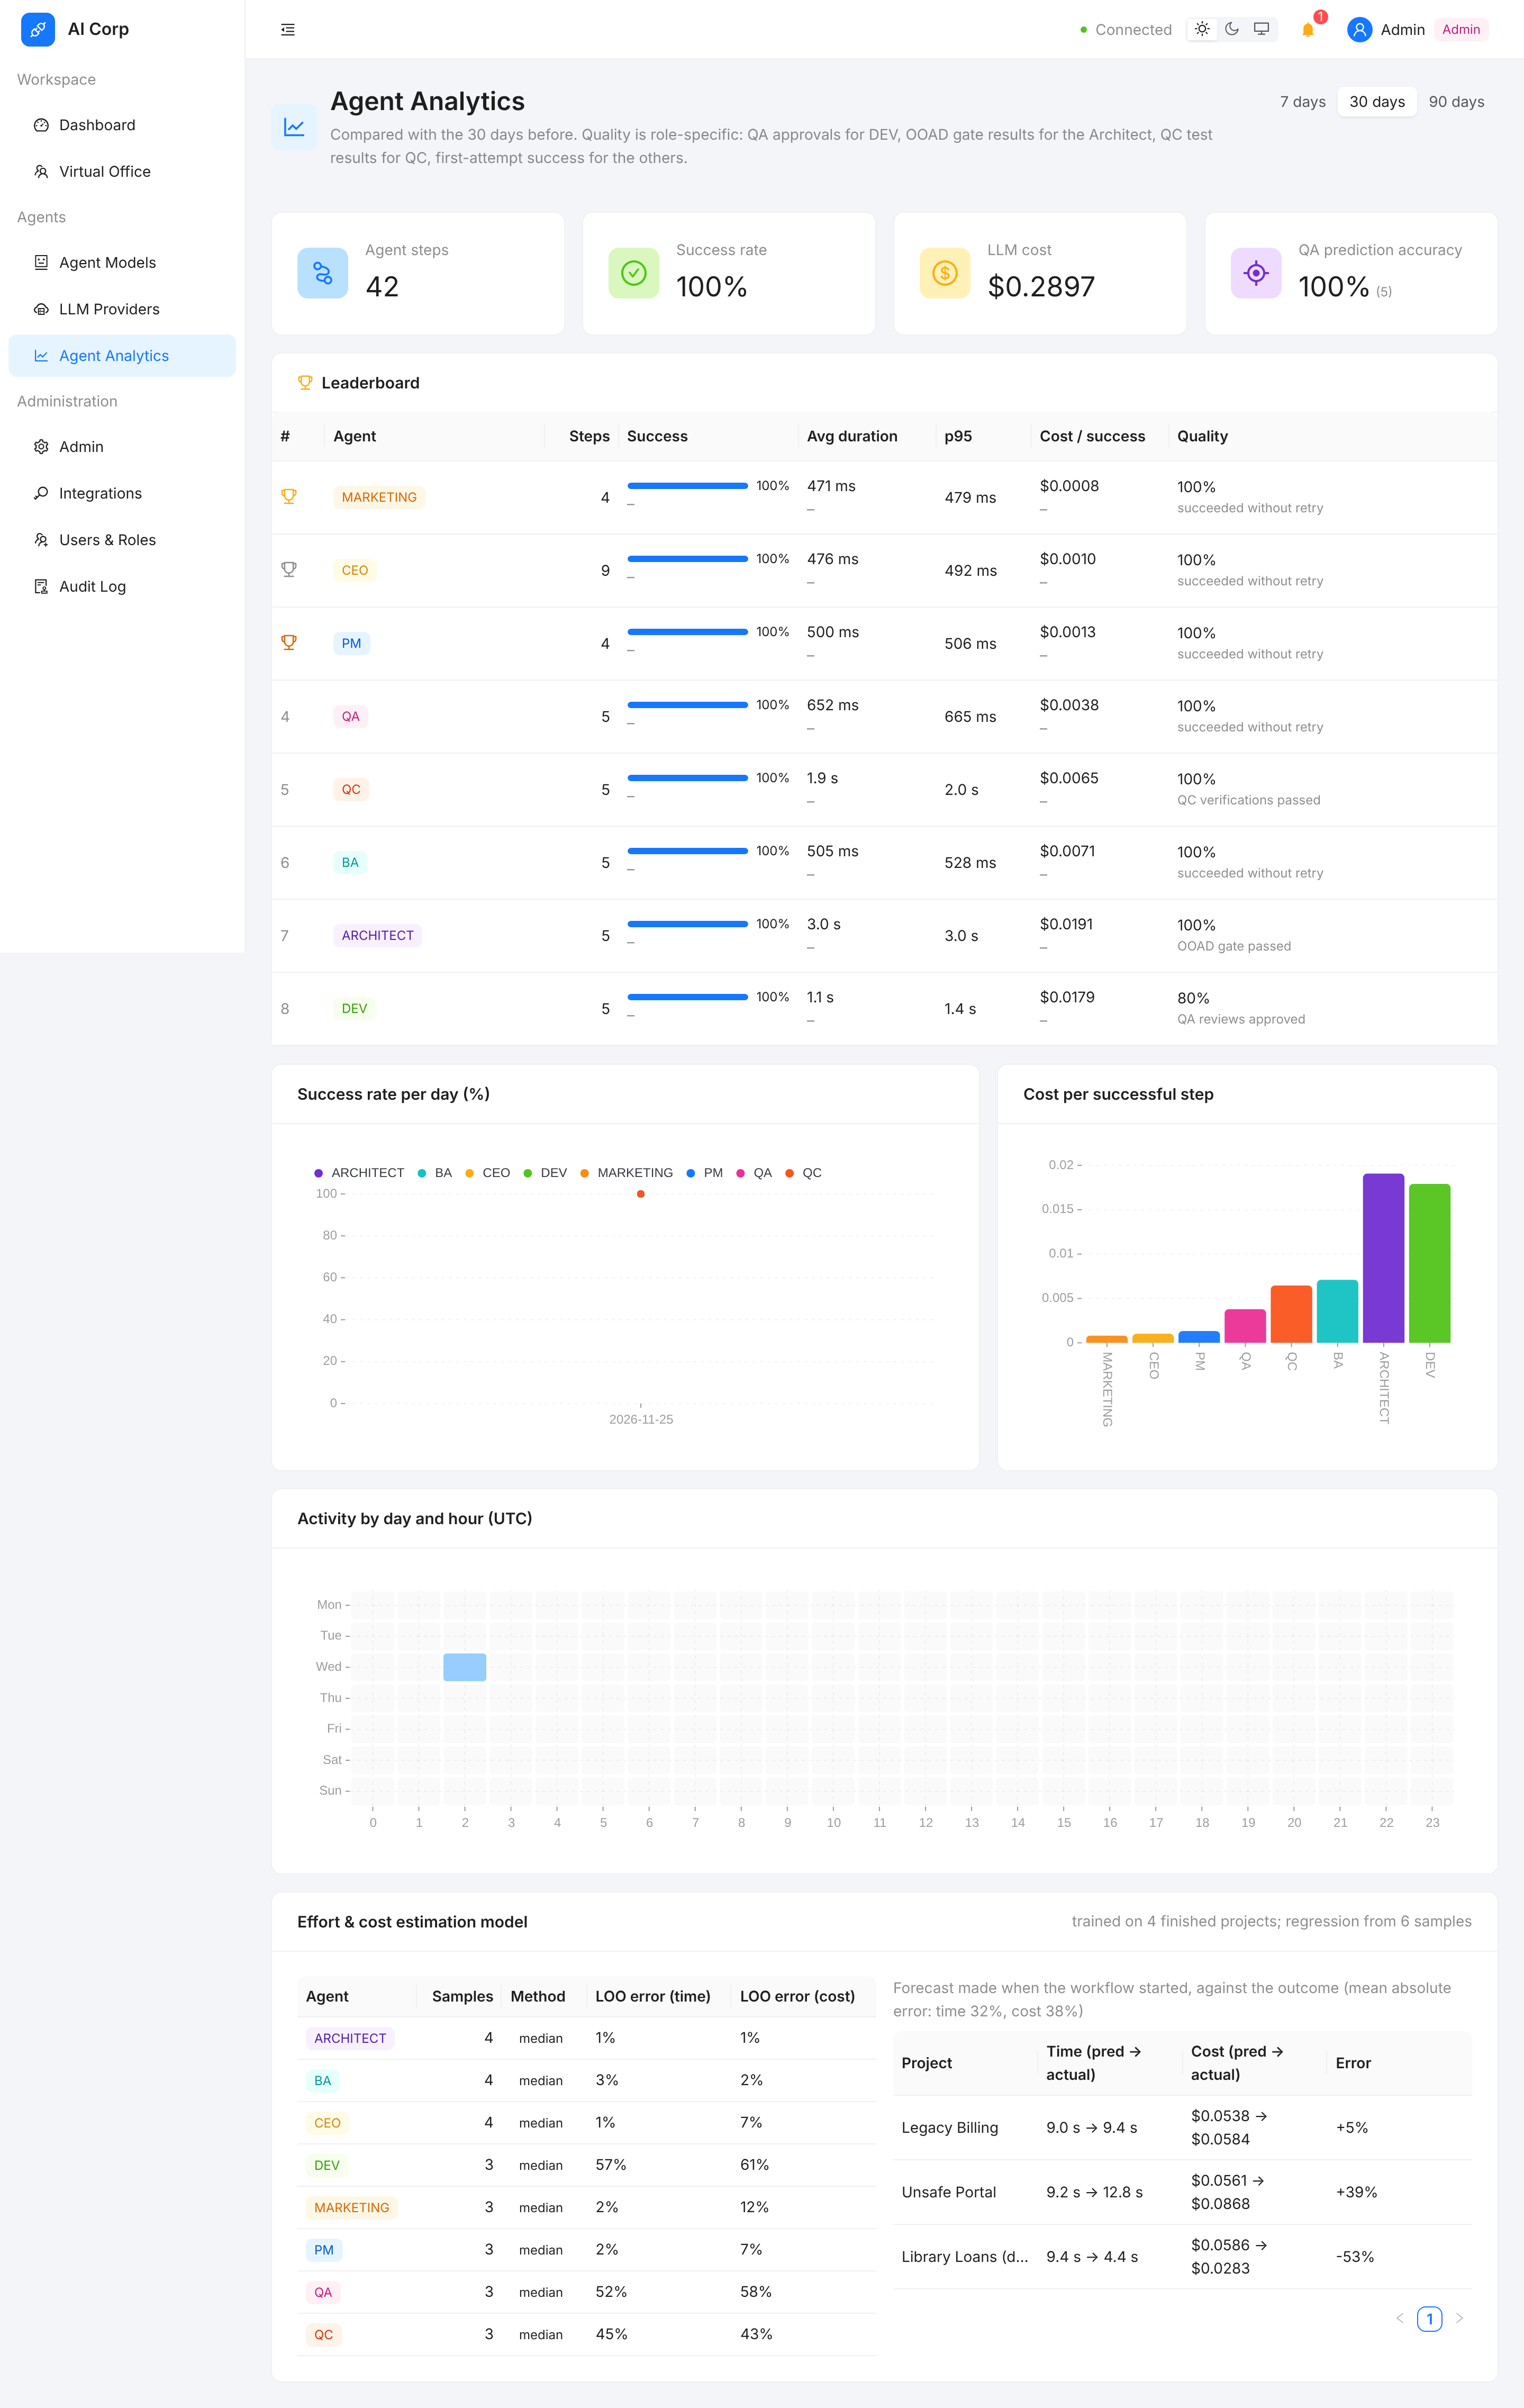
\includegraphics[height=0.75\textheight]{anh/agent-analytics.png}
\end{figure}


\end{document}
